% =========================================================
% University of Toronto MSc Thesis (SGS-aligned ut-thesis class)
% =========================================================
\documentclass[
  11pt,
  letterpaper,
  onehalfspacing,
  normalmargins,
  equalmargins,
  oneside
]{ut-thesis}

% -------- Packages --------
% Encoding & micro-typography
\usepackage[T1]{fontenc}
\usepackage[utf8]{inputenc}  % pdfLaTeX
\usepackage[final]{microtype}
\usepackage{setspace}

% Math
\usepackage{amsmath,amssymb,amsfonts}
\newtheorem{notation}{Notation}
\usepackage{mathtools}
\usepackage{bm}
\usepackage{braket}
% Figures, colors, links
\usepackage{graphicx}
\usepackage{comment}
\usepackage[dvipsnames]{xcolor}
\usepackage{subcaption}
\usepackage[hidelinks]{hyperref}
\usepackage[nameinlink,noabbrev]{cleveref} % load AFTER hyperref
\hypersetup{
  pdftitle={Gaussian-Process Reconstruction of the Mapping-QCLE Excess Term: A Moving-Cloud Formulation and Failure Analysis},
  pdfauthor={Sahand Nikzat},
  pdfsubject={Master of Science thesis, Graduate Department of Chemistry, University of Toronto},
  pdfkeywords={quantum-classical Liouville equation, mapping basis, Gaussian processes, nonadiabatic dynamics},
  pdfdisplaydoctitle=true
}
\usepackage{tabularx}
\usepackage{longtable}
\usepackage{pdflscape}
\usepackage{array}
\usepackage{float}
\usepackage{placeins}

\newcolumntype{Y}{>{\raggedright\arraybackslash}X}
\newcolumntype{L}[1]{>{\raggedright\arraybackslash}p{#1}}
% Tables & units (optional but common in physics)
\usepackage{booktabs}
\usepackage{siunitx}
\sisetup{separate-uncertainty,detect-all}

% Bibliography (pick one route; natbib shown below)
\usepackage[numbers,sort&compress]{natbib}

% List of Appendices, included because this thesis contains an appendix.
\makeatletter
\newcommand{\listappendixname}{List of Appendices}
\newcommand{\listofappendices}{%
  \chapter*{\listappendixname}%
  \@starttoc{loa}%
}
\newcommand*{\l@appendix}{\@dottedtocline{0}{0em}{4em}}
\makeatother

% -------- Mandatory SGS front-matter metadata --------
\title{Gaussian-Process Reconstruction of the Mapping-QCLE Excess Term: A Moving-Cloud Formulation and Failure Analysis}
\author{Sahand Nikzat}
\degree{Master of Science}
\department[Graduate Department of]{Chemistry}
\gradyear{2026}
\copyrighttext{{\copyright} Copyright by Sahand Nikzat 2026}

% Optional: keywords, additional info (some styles ignore these)
% \keywords{quantum-classical Liouville equation, mapping basis, Gaussian processes}

\begin{document}

% -------- Front matter (roman numbering) --------
\frontmatter
\maketitle

\begin{abstract}
\label{sec:abstract}
\begin{onehalfspace}
Nonadiabatic molecular dynamics requires coupled treatment of electronic transitions and nuclear motion. The mapping-basis quantum--classical Liouville equation supplies this treatment, but its density-dependent correction requires costly mixed phase-space derivatives on multidimensional grids. This thesis tests whether a Gaussian-process model can recover the density and these derivatives from a moving trajectory cloud. A Hamiltonian scheme transports the cloud, while an explicit midpoint update applies the correction. For a one-dimensional, two-state avoided-crossing model, validation uses analytic operator tests, refinement and conservation checks, replicates, and comparison with numerically controlled reference solutions of the time-dependent Schrödinger equation and grid-based quantum--classical Liouville equation. Density values are reconstructed accurately, but derivative errors do not decrease consistently; the model violates electronic-state constraints, exhibits normalization and energy drift, and varies across replicates. Consequently, the formulation does not reliably improve the Poisson-bracket mapping equation, but establishes derivative-fidelity, structural, and conservation requirements for a viable successor.

\end{onehalfspace}
\end{abstract}

\begin{acknowledgements}
I am deeply grateful to my parents, whose support sustained me throughout my years abroad. Moving from my homeland to a new country brought profound cultural differences and many challenges, especially after I came to Canada for graduate studies. Dear Mom, your love kept my spirit alive; I could not have continued through the darkest moments without your compassionate words and unwavering encouragement. Dear Dad, I have always tried not to disappoint you. Thank you for standing by me through the hardest decisions of my life. As you often say: the darkest hours do come, yet the LORD knows how to shine His light into our lives. I also remember the Rumi poem you would read to me:
\begin{quote}
``Who looks out with my eyes? What is the soul?\\
I cannot stop asking.\\
If I could taste one sip of an answer,\\
I could break out of this prison for drunks.''
\end{quote}
\begin{flushright}
\emph{---Rumi, translated by Coleman Barks}
\end{flushright}

I especially thank my supervisor, Professor Jeremy Schofield, for recognizing both my strengths and my weaknesses, and for guiding me with insight and patience. Only a truly thoughtful advisor can engage with a student's scientific viewpoint and create space for it to flourish. His exceptional knowledge continually pushed me to explore new ideas, to confront my limitations, and to turn them into strengths. During the writing of this thesis, he passed away. May his soul rest in peace. His light will always be with me.

I am also grateful to my colleague and friend, Kai Gu, for many thoughtful discussions and the generous exchange of ideas and perspectives on our projects. Those conversations sharpened my thinking and improved this work.

To all who offered guidance, friendship, and encouragement along the way---thank you. In particular, I thank Seyedreza Rezaiee, Vesal Kasmaeifar, Ahamadreza Khazaeipoul, and Mohammadreza JangRouei for their friendship and support, and I wish them an exciting and successful journey through their graduate studies.
\end{acknowledgements}

\begin{comment}
\chapter*{Preface: Research Philosophy}
\addcontentsline{toc}{chapter}{Preface: Research Philosophy}

Chemical physics is often introduced through structure: molecular geometries,
potential-energy surfaces, electronic states, and stationary configurations.
These objects are indispensable, but they are not the whole story. Many
chemical phenomena are determined not only by where a molecule can be, but by
how it moves between possibilities. A reaction pathway, an electronic
transition, a transfer event, or a relaxation process is not simply a point on
a surface. It is a dynamical event in which electronic character, nuclear
motion, and environmental response evolve together.

This thesis is built around that viewpoint. The central object is not a static
molecular structure, but an evolving quantum--classical density. In
nonadiabatic dynamics, electronic populations and coherences are coupled to
nuclear motion, and the environment can reshape energy gaps, alter couplings,
and suppress phase information. A useful theory must therefore do more than
label electronic states or propagate representative trajectories. It must
describe how probability, phase, and energy move through the coupled
electronic--nuclear system.

The adiabatic approximation provides one of the most powerful organizing ideas
in molecular quantum mechanics. It begins by solving the electronic problem at
fixed nuclear geometry and then uses the resulting electronic energies as
surfaces for nuclear motion. This picture explains much of molecular structure
and reactivity. Its limitation, however, is equally important. When electronic
states become close in energy or when the electronic basis changes rapidly with
nuclear geometry, the neglected coupling terms become dynamically relevant.
The molecule can no longer be understood as moving on one electronic surface
alone. This failure of the adiabatic picture is not a technical inconvenience;
it is the origin of many of the most important phenomena in nonadiabatic
chemical dynamics.

Different representations expose different aspects of this problem. In an
adiabatic representation, nonadiabatic effects appear through derivative
couplings generated by nuclear motion. In a diabatic representation, the same
physics appears through off-diagonal electronic couplings between chemically
meaningful configurations. Neither representation is the truth by itself. Each
is a language for organizing the same coupled quantum dynamics. The guiding
principle is therefore not to privilege one picture blindly, but to preserve
the structure of the underlying equation as faithfully as possible.

This principle also shapes the computational philosophy of the thesis. Many
trajectory-based methods are valuable because they make high-dimensional
molecular dynamics tractable. However, a set of trajectories is not itself the
density. When the governing equation contains terms that depend on derivatives
or integrals of the density, the density must be represented explicitly and
carefully. Otherwise, important physical information can be hidden in sampling
noise, numerical differentiation, or uncontrolled reconstruction procedures.

The work developed here treats the phase-space density as the primary object.
The role of trajectories is to provide dynamically relevant support, but the
role of the Gaussian-process surrogate is to reconstruct a smooth,
differentiable, and physically constrained representation of the density carried
by that support. In this sense, statistics enters in service of dynamics. The
Gaussian process is not introduced to replace the molecular Hamiltonian or to
learn dynamics as an unconstrained black box. It is introduced because the
quantum--classical Liouville operator requires access to a density that can be
differentiated, integrated, monitored, and corrected in a controlled way.

This distinction is essential. The goal is not merely to improve numerical
fits, but to respect the mathematical and physical structure of the problem.
Normalization, energy behavior, trace consistency, electronic populations,
coherences, density negativity, and uncertainty are not secondary diagnostics;
they are signs of whether the representation remains faithful to the dynamics
it is meant to approximate. A surrogate that fits data while violating these
structures is not a satisfactory physical model. A useful surrogate must carry
the density in a way that allows the operator, not the fitting procedure, to
dictate the evolution.

The mapping representation provides the setting for this program. By encoding
discrete electronic states in continuous mapping variables, it places
electronic populations and coherences into a phase-space framework. The
Poisson-bracket mapping equation captures the leading Hamiltonian-like
transport, but the full mapping-basis quantum--classical Liouville equation
contains additional terms that are difficult to evaluate from raw trajectory
ensembles alone. The central motivation of this thesis is to make those
density-dependent terms computationally accessible without abandoning the
operator structure from which they arise.

The broader philosophy is therefore structure before approximation. First
identify the exact or systematic equation that expresses the physics. Then ask
which parts of the equation are computationally difficult. Approximate only
what must be approximated, and do so in a way that preserves the quantities
that make the model physically meaningful. In this work, the difficult object
is the evolving mapping-basis density. The approximation is the
Gaussian-process representation of that density. The dynamics, the couplings,
and the conservation principles remain the organizing constraints.

This thesis is an attempt to bring together three perspectives that are often
treated separately: the chemical intuition of pathways and electronic-state
mixing, the physical structure of quantum--classical Liouville dynamics, and
the statistical discipline of uncertainty-aware density reconstruction. The
aim is not only to generate trajectories, but to understand how a
nonadiabatic density evolves, where the approximation is reliable, and where
the dynamics demands additional resolution. In that sense, the work follows a
simple principle: computation should not obscure the physics it was built to
represent.
\end{comment}
\tableofcontents
\listoftables
\listofappendices

\chapter*{Abbreviations}
\phantomsection
\addcontentsline{toc}{chapter}{Abbreviations}
\markboth{Abbreviations}{Abbreviations}

\begin{tabularx}{\textwidth}{@{}L{0.18\textwidth}Y@{}}
\toprule
\textbf{Abbreviation} & \textbf{Meaning} \\
\midrule
ARD & automatic relevance determination \\
ESS & effective sample size \\
GP & Gaussian process \\
KDE & kernel density estimation \\
LOO & leave-one-out \\
MInt & Momentum Integral \\
MMST & Meyer--Miller--Stock--Thoss \\
NMLL & negative marginal log likelihood \\
PBME & Poisson-bracket mapping equation \\
QCLE & quantum--classical Liouville equation \\
RBF & radial basis function \\
SEO & singly excited oscillator \\
TDSE & time-dependent Schr\"odinger equation \\
\bottomrule
\end{tabularx}

% ============================================================
% NOTATION AND CONVENTIONS
% Place after \listoftables and before \mainmatter
% ============================================================

\chapter*{Notation and Conventions}
\phantomsection
\addcontentsline{toc}{chapter}{Notation and Conventions}
\markboth{Notation and Conventions}{Notation and Conventions}
\label{sec:global-notation-conventions}

This thesis combines fully quantum molecular notation, quantum--classical
phase-space notation, MMST mapping variables, and Gaussian-process regression.
The conventions summarized below are used throughout the thesis. Symbols
introduced for a specialized calculation retain these meanings unless an
explicit local qualification is stated.

\begingroup
\small
\renewcommand{\arraystretch}{1.18}
\setlength{\tabcolsep}{4pt}

\begin{longtable}{
@{}
>{\raggedright\arraybackslash}p{0.19\textwidth}
>{\raggedright\arraybackslash}p{0.23\textwidth}
>{\raggedright\arraybackslash}p{0.49\textwidth}
@{}
}

\caption{Canonical notation and conventions used throughout the thesis.}
\label{tab:canonical-notation}\\

\toprule
\textbf{Mathematical object}
&
\textbf{Canonical notation}
&
\textbf{Convention}
\\
\midrule
\endfirsthead

\multicolumn{3}{c}{
\tablename\ \thetable\ -- continued from the previous page
}
\\
\toprule
\textbf{Mathematical object}
&
\textbf{Canonical notation}
&
\textbf{Convention}
\\
\midrule
\endhead

\midrule
\multicolumn{3}{r}{Continued on the next page}
\\
\endfoot

\bottomrule
\endlastfoot

% ------------------------------------------------------------
% Coordinates and phase-space variables
% ------------------------------------------------------------

\multicolumn{3}{@{}l}{
\textbf{Coordinates and phase-space variables}
}
\\
\addlinespace[0.3em]

Electronic coordinates
&
\(\mathbf q=(\mathbf q_1,\ldots,\mathbf q_{N_e})\)
&
Used exclusively for fully quantum electronic coordinates in
Chapter~\ref{chap:introduction}.
\\

Nuclear or bath coordinates and momenta
&
\(\mathbf R,\mathbf P\)
&
The bath phase-space point is
\(\mathbf X=(\mathbf R,\mathbf P)\).
\\

Common bath mass
&
\(M\)
&
A scalar common bath mass is used in the quantum--classical and mapping
models:
\[
T_{\mathrm b}(\mathbf P)=\frac{\mathbf P^2}{2M},
\qquad
\dot{\mathbf R}=\frac{\mathbf P}{M}.
\]
Individual molecular nuclear masses in the fully quantum discussion are
denoted by \(M_A\).
\\

Mapping coordinates and momenta
&
\(\mathbf r,\mathbf p\)
&
The mapping phase-space point is
\(\mathbf x=(\mathbf r,\mathbf p)\).
\\

Extended bath--mapping phase-space point
&
\(\boldsymbol{\mathcal X}=(\mathbf X,\mathbf x)\)
&
Equivalently,
\[
\boldsymbol{\mathcal X}
=
(\mathbf R,\mathbf P,\mathbf r,\mathbf p).
\]
This notation is used from
Chapter~\ref{chap:mapping-representation} onward.
\\

% ------------------------------------------------------------
% Index conventions
% ------------------------------------------------------------

\addlinespace[0.6em]
\multicolumn{3}{@{}l}{
\textbf{Index conventions}
}
\\
\addlinespace[0.3em]

Adiabatic-state indices
&
\(\alpha,\beta,\alpha',\beta'\)
&
Reserved for adiabatic electronic states and adiabatic-basis QCLE matrix
elements.
\\

Fixed-basis and mapping-state indices
&
\(\lambda,\lambda',\kappa,\kappa'\)
&
Reserved for states in the fixed subsystem basis and for the corresponding
MMST mapping oscillators. For a subsystem with \(N_s\) states,
\[
\lambda,\lambda',\kappa,\kappa'
\in\{1,\ldots,N_s\}.
\]
\\

Support-point and kernel-centre indices
&
\(i,j\)
&
Index GP support points, physical density labels, kernel centres, and
kernel-expansion terms.
\\

Local MInt eigenmode indices
&
\(a,b\)
&
Used only for the temporary local diagonalization of the fixed-basis
subsystem Hamiltonian during an MInt substep.
\\

% ------------------------------------------------------------
% Quantum-classical densities
% ------------------------------------------------------------

\addlinespace[0.6em]
\multicolumn{3}{@{}l}{
\textbf{Quantum--classical and mapping densities}
}
\\
\addlinespace[0.3em]

Mass-separation parameter
&
\(\varepsilon_m=\sqrt{m/M}\)
&
Used only in the QCLE mass-ratio expansion. The symbol \(\mu_t\) is reserved
for the GP posterior mean or modulation function.
\\

Partially Wigner-transformed density operator
&
\(\hat\rho_W(\mathbf X,t)\)
&
Operator-valued in the finite subsystem Hilbert space and defined over the
bath phase space.
\\

Subsystem matrix elements of the Wigner density
&
\(\rho_W^{\lambda\lambda'}(\mathbf X,t)\)
&
Fixed-basis matrix elements of
\(\hat\rho_W(\mathbf X,t)\).
Adiabatic-basis matrix elements use adiabatic indices,
for example \(\rho_W^{\alpha\beta}\).
\\

Exact projected mapping density
&
\(\widetilde\rho_m(\boldsymbol{\mathcal X},t)\)
&
The physical SEO-projected mapping density derived in
Chapter~\ref{chap:mapping-representation}.
\\

Numerical mapping-density surrogate
&
\(\widehat\rho_{m,t}(\boldsymbol{\mathcal X})\)
&
A fixed-time numerical approximation to
\(\widetilde\rho_m(\boldsymbol{\mathcal X},t)\).
\\

Structured product surrogate
&
\(\widehat\rho_{m,t}=g_s\mu_t\)
&
The physical SEO profile \(g_s(\mathbf x)\) is multiplied by the smooth
GP modulation function \(\mu_t(\boldsymbol{\mathcal X})\).
\\

Physical density labels
&
\(\mathbf y_t\) or \(\mathbf y^{\,n}\)
&
Values of the complete mapping density carried by the dynamically
transported support cloud:
\[
y_i^n
\approx
\widetilde\rho_m
\left(
\boldsymbol{\mathcal X}_i^n,t_n
\right).
\]
\\

Transformed modulation labels
&
\(\mathbf u_t\) or \(\mathbf u^{\,n}\)
&
Safe-profile ratios used as GP regression targets:
\[
u_i^n
=
\frac{y_i^n}
{g_{s,\mathrm{safe}}(\mathbf x_i^n)}.
\]
\\

GP kernel coefficients
&
\(\boldsymbol\zeta_t\) or
\(\boldsymbol\zeta^{\,n}\)
&
Defined by the regularized kernel solve
\[
\boldsymbol\zeta_t
=
K_{y,t}^{-1}\mathbf u_t
\]
for the product representation.
\\

Regularized kernel matrix
&
\(K_{y,t}\)
&
Defined by
\[
K_{y,t}
=
K_t+\sigma_n^2 I,
\]
with any numerical jitter included in the diagonal regularization.
\\

GP precision matrix
&
\(\mathsf P_t=K_{y,t}^{-1}\)
&
Used in leave-one-out formulas and distinguished from all source-generator
matrices.
\\

GP support set
&
\(\mathcal S_t\) or \(\mathcal S_n\)
&
The time-dependent set of support points:
\[
\mathcal S_n
=
\left\{
\boldsymbol{\mathcal X}_i^n
\right\}_{i=1}^{N}.
\]
\\

% ------------------------------------------------------------
% Hamiltonians and Liouvillians
% ------------------------------------------------------------

\addlinespace[0.6em]
\multicolumn{3}{@{}l}{
\textbf{Hamiltonians, Liouvillians, and propagators}
}
\\
\addlinespace[0.3em]

Subsystem Hamiltonian
&
\(h(\mathbf R)\)
&
The finite-dimensional subsystem Hamiltonian in the fixed basis.
Its matrix elements are \(h^{\lambda\lambda'}(\mathbf R)\).
\\

Trace--traceless decomposition
&
\(h(\mathbf R)=\eta(\mathbf R)I_s+\bar h(\mathbf R)\)
&
The scalar trace contribution is incorporated into the state-independent
bath potential \(V_0(\mathbf R)\), while
\[
\operatorname{Tr}_s\bar h(\mathbf R)=0.
\]
\\

Mapping Hamiltonian
&
\(H_m(\boldsymbol{\mathcal X})\)
&
The MMST mapping Hamiltonian generating the PBME characteristic flow.
\\

Hamiltonian mapping Liouvillian
&
\(i\mathcal L_m^\circ\)
&
Its density generator is
\[
\mathcal T=-i\mathcal L_m^\circ.
\]
\\

Excess mapping Liouvillian
&
\(i\mathcal L_m'\)
&
Its density source is
\[
\mathcal Q=-i\mathcal L_m'.
\]
For one bath coordinate,
\[
\mathcal Q[f]
=
-\frac{\hbar}{8}
\sum_{\lambda,\lambda'}
\frac{d\bar h^{\lambda\lambda'}}{dR}
\left(
\partial_{r_{\lambda'}}
\partial_{r_\lambda}
+
\partial_{p_{\lambda'}}
\partial_{p_\lambda}
\right)
\partial_P f.
\]
\\

PBME/MInt flow map
&
\(\Psi_\tau^{\mathrm{MInt}}\)
&
The numerical map approximating the Hamiltonian PBME flow over a time
interval \(\tau\).
\\

Transport propagator
&
\(\mathcal U_\tau^{\mathrm T}\)
&
Propagates the support cloud under the PBME/MInt transport leg.
\\

Source propagator
&
\(\mathcal U_\tau^{\mathrm Q}\)
&
Propagates the density or transformed labels under the excess
mapping-QCLE source leg.
\\

Complete symmetric step
&
\(\mathcal U_{\Delta t}^{\mathrm{TST}}\)
&
Defined by
\[
\mathcal U_{\Delta t}^{\mathrm{TST}}
=
\mathcal U_{\Delta t/2}^{\mathrm T}
\mathcal U_{\Delta t}^{\mathrm Q}
\mathcal U_{\Delta t/2}^{\mathrm T}.
\]
\\

% ------------------------------------------------------------
% Discrete source matrices
% ------------------------------------------------------------

\addlinespace[0.6em]
\multicolumn{3}{@{}l}{
\textbf{Discrete source matrices}
}
\\
\addlinespace[0.3em]

Product basis function
&
\(\Phi_j(\boldsymbol{\mathcal X})=g_s(\mathbf x)k_j(\boldsymbol{\mathcal X})\)
&
The physical basis on which the excess source is collocated.
\\

Discrete physical source matrix
&
\(\mathsf L^{(\rho)}\)
&
Defined by
\[
\mathsf L^{(\rho)}_{ij}
=
\left.
\mathcal Q[\Phi_j]
\right|_{\boldsymbol{\mathcal X}_i}.
\]
\\

Safe-profile diagonal matrix
&
\(\mathsf D_g\)
&
Defined by
\[
\mathsf D_g
=
\operatorname{diag}
\left[
g_{s,\mathrm{safe}}(\mathbf x_i)
\right].
\]
\\

Discrete modulation source matrix
&
\(\mathsf L\)
&
Defined by
\[
\mathsf L
=
\mathsf D_g^{-1}\mathsf L^{(\rho)}.
\]
\\

Frozen modulation generator
&
\(\mathsf A=\mathsf L K_y^{-1}\)
&
Generates the frozen source-leg equation
\[
\frac{d\mathbf u}{dt}
=
\mathsf A\mathbf u.
\]
\\

% ------------------------------------------------------------
% Mapping observables and invariants
% ------------------------------------------------------------

\addlinespace[0.6em]
\multicolumn{3}{@{}l}{
\textbf{Mapping observables, invariants, and diagnostics}
}
\\
\addlinespace[0.3em]

Mapping observable symbol
&
\(c_{\lambda\lambda'}(\mathbf x)\)
&
MMST phase-space symbol of the subsystem operator
\(\lvert\lambda\rangle\langle\lambda'\rvert\).
\\

Mapped identity symbol
&
\(I_m(\mathbf x)\)
&
The MMST phase-space symbol of the subsystem identity:
\[
I_m(\mathbf x)
=
\sum_{\lambda=1}^{N_s}
c_{\lambda\lambda}(\mathbf x).
\]
\\

Mapping-radius invariant
&
\(\mathcal R_m^2(\mathbf x)\)
&
Defined by
\[
\mathcal R_m^2(\mathbf x)
=
\mathbf r^T\mathbf r
+
\mathbf p^T\mathbf p.
\]
It is conserved by the MInt Hamiltonian mapping rotation.
\\

Raw density integral
&
\(\mathcal N_{\mathrm{raw}}(t)\)
&
The full phase-space integral of the complete mapping-density surrogate:
\[
\mathcal N_{\mathrm{raw}}(t)
=
\int
d\boldsymbol{\mathcal X}\,
\widehat\rho_{m,t}
(\boldsymbol{\mathcal X}).
\]
\\

Subsystem trace diagnostic
&
\(\mathcal N_{\mathrm{tr}}(t)\)
&
Computed using the mapped identity or diagonal mapping observable symbols:
\[
\mathcal N_{\mathrm{tr}}(t)
=
\int
d\boldsymbol{\mathcal X}\,
I_m(\mathbf x)
\widehat\rho_{m,t}
(\boldsymbol{\mathcal X}).
\]
\\

Physical energy
&
\(\mathcal E(t)\)
&
The density-weighted expectation of the physical mapping Hamiltonian or
the corresponding physical energy observable.
\\

\end{longtable}

\endgroup

% -------- Main matter (arabic numbering) --------
\mainmatter

\chapter{Introduction}
\label{chap:introduction}

This thesis tests one specific numerical construction: a product-GP density on
moving PBME/MInt support, analytic evaluation of the mapping-QCLE excess
source, and an explicit midpoint update of the live density labels for the
one-dimensional, two-state avoided-crossing benchmark. It does not test all
Gaussian-process representations or all discretizations of the continuum
mapping-QCLE excess term. Reconstruction, derivative-operator fidelity, SEO
projection, conservation, refinement, stochastic replication, and comparison
with physical references are tested separately so that a completed calculation
is not mistaken for a validated method.  The resulting evidence is negative:
the tested construction does not satisfy the joint conditions and does not
demonstrate systematic improvement over PBME.  Its contribution is therefore
the formulation, the controlled failure analysis, and the design requirements
that follow from it.

\section{Motivation and scope}
\label{sec:introduction-motivation-scope}

The mapping-basis quantum--classical Liouville equation (QCLE) provides a more
complete mixed quantum--classical description than the Poisson-bracket mapping
equation (PBME), but its excess term acts through mixed derivatives of a signed
phase-space density. Direct evaluation on a multidimensional grid becomes
prohibitively expensive as the number of environmental coordinates increases,
whereas PBME achieves trajectory-level cost by discarding the term. The
resulting tension between physical completeness and computational feasibility
motivates this thesis: a moving trajectory cloud is used to locate dynamically
relevant regions of phase space, and a Gaussian-process (GP) density
representation is used to supply the differentiable field required by the
excess operator.

For this benchmarked construction, usefulness would require an improvement of
the QCLE approximation rather than merely a smooth interpolation. Its evaluation therefore
requires four connected forms of evidence: accurate reconstruction of a
manufactured excess operator, time-step sensitivity and independent-cloud
enlargement, preservation of the singly-excited-oscillator (SEO) projected
structure and physical moments, and smaller errors than PBME against
independently resolved quantum and grid-QCLE references. These requirements
provide the scientific acceptance criteria for the numerical study.

The calculations show that the tested representation does not satisfy those
criteria.  Its manufactured excess-operator error is non-monotone under the
tested enlargement, the product surrogate develops substantial leakage from
the physical SEO image, and four-seed MIDPOINT calculations show severe
dispersion and raw normalization drift.  No validated evidence of systematic
improvement over PBME was obtained.

The general fact that on-manifold values do not determine ambient normal
derivatives is not claimed as new.  The distinctive contribution is instead a
specific
moving-cloud density-level implementation and controlled test: it formulates
the excess update on PBME/MInt support, contrasts the product surrogate with
the exact four-real-field SEO image, measures projection leakage, demonstrates
derivative-operator failure despite small value errors, and connects that
evidence to nonconservative collocation and signed-weight collapse.  Previous
mapping-QCLE work established the projected mapping equations and PBME
approximation \cite{Kim2008JCP,Kelly2012JCP}, while numerical GP and meshfree
work established differentiable surrogate tools
\cite{Solak2002DerivativeGP,Raissi2017LinearGP,
CockayneOatesSullivanGirolami2019}; the original contribution here is their particular
moving-cloud product-GP realization and application-specific failure
diagnosis, stated without an unsupported priority claim.

This conclusion is deliberately restricted to the one-dimensional, two-state
Tully dual avoided-crossing benchmark studied here. The model is sufficiently
controlled to separate reference, reconstruction, operator, integration, and
sampling errors, but it cannot establish general accuracy or scalability for
multidimensional molecular systems.

Molecular dynamics in condensed phases is often governed by events that cannot
be inferred from equilibrium molecular structures alone. Many chemical and
material processes involve the coupled evolution of electronic populations,
nuclear coordinates, energy redistribution, and environmental fluctuations.
Charge transfer, exciton migration, photochemical relaxation,
proton-coupled reactions, catalytic bond rearrangement, electrochemical
transformations, and energy transport in molecular materials all depend on the
simultaneous evolution of electronic, nuclear, and environmental degrees of
freedom
\cite{Curchod2018ChemRev,CrespoOtero2018ChemRev,Kapral2006ARPC,
Tully2012Perspective,Subotnik2016AnnualReview,Kapral2015JPCM}.

The central theoretical difficulty is that these processes often occur outside
the range of validity of a strictly adiabatic description. In the
Born--Oppenheimer picture, the nuclei evolve on a single electronic
potential-energy surface while the electronic state adjusts parametrically to
the nuclear configuration \cite{BornOppenheimer1927,BornHuang1954}. This
separation is powerful when electronic states remain well separated in energy
and the electronic basis varies slowly with nuclear geometry. It becomes
inadequate, however, when nuclear motion carries the system through regions
where two or more electronic states are close in energy or strongly coupled.
Avoided crossings, conical intersections, charge-transfer resonances,
bond-breaking regions, fluctuating solvent configurations, and strongly
reorganizing molecular environments can all generate such conditions
\cite{Yarkony1996RMP,Baer2006Book}. In these regimes, nuclear motion may
induce transitions between electronic states, while the evolving electronic
state modifies the forces acting on the nuclei.

This is the regime of nonadiabatic molecular dynamics. Its importance is not
restricted to one class of experiments or one chemical example. In
electron-transfer systems, environmental reorganization can tune donor and
acceptor states into resonance. In molecular aggregates and materials, nuclear
fluctuations can control the migration, localization, and relaxation of
electronic excitation. In photochemical reactions, passage through strongly
coupled regions of configuration space can determine whether a molecule
relaxes, isomerizes, dissociates, or branches into competing product channels.
In proton-coupled and hydrogen-transfer processes, light-particle motion,
electronic redistribution, and environmental polarization may become
inseparable. These examples differ chemically, but they share a common
theoretical requirement: electronic quantum dynamics and nuclear or
environmental motion must be treated as coupled parts of the same dynamical
process.

Fully quantum dynamics provides the reference description in principle, but it
is generally infeasible for condensed-phase systems with many nuclear degrees
of freedom. Mixed quantum--classical methods offer a practical compromise by
treating selected electronic or subsystem degrees of freedom quantum
mechanically while representing the surrounding nuclear environment with
classical phase-space variables. Methods such as Ehrenfest dynamics,
trajectory surface hopping, and linearized semiclassical approaches have
provided important insight, but each introduces approximations whose
consequences must be examined when coherence, decoherence, detailed balance,
nuclear back-reaction, or long-time propagation are important
\cite{Tully1990JCP,Kapral2006ARPC,Curchod2018ChemRev}.

The quantum--classical Liouville equation provides a systematic density-level
starting point for this problem. It describes the coupled evolution of a
quantum subsystem and a classical bath while retaining the subsystem density
matrix, nuclear phase-space variables, and their mutual back-reaction within a
mixed quantum--classical framework
\cite{KapralCiccotti1999JCP,Kapral2006ARPC}. In the mapping representation,
discrete subsystem states are represented by continuous mapping variables,
placing populations, coherences, nuclear coordinates, nuclear momenta, and
mapping variables within a unified phase-space formulation
\cite{MeyerMiller1979JCP,StockThoss1997PRL,Kim2008JCP}.

The scope of this introductory chapter is to build the conceptual path toward
that formulation. The chapter begins with the adiabatic approximation and its
breakdown, then discusses adiabatic and diabatic representations,
potential-energy surfaces, density matrices, subsystem--bath coupling,
Landau--Zener transitions, and the Wigner phase-space representation. These
ingredients provide the background needed to formulate the thesis objective:
the construction and controlled assessment of one product-Gaussian-process
density representation on PBME/MInt-transported support, coupled to an
explicit MIDPOINT live-label update, for the mapping-basis quantum--classical
Liouville equation on a one-dimensional two-state benchmark.


\section{The adiabatic approximation and its breakdown}
\label{sec:adiabatic-approximation-breakdown}

The microscopic starting point for molecular quantum dynamics is the
nonrelativistic molecular Hamiltonian. For a system of \(N_e\) electrons and
\(N_n\) nuclei, let
\[
\mathbf q=(\mathbf q_1,\ldots,\mathbf q_{N_e})
\]
denote the electronic coordinates and
\[
\mathbf R=(\mathbf R_1,\ldots,\mathbf R_{N_n})
\]
denote the nuclear coordinates. In the Born--Oppenheimer construction, the
electronic problem is solved at fixed nuclear configuration. To make this
conditional structure explicit, electronic quantities will be written with the
notation \(\mathbf q\mid\mathbf R\). Thus
\(\phi_\alpha(\mathbf q\mid\mathbf R)\) denotes an electronic wavefunction in
the electronic coordinates \(\mathbf q\), parametrically conditioned on the
nuclear geometry \(\mathbf R\).

Neglecting relativistic corrections, spin-dependent interactions, and external
fields, the molecular Hamiltonian can be written as
\begin{equation}
\hat H
=
\hat T_{\mathrm n}
+
\hat H_{\mathrm e}(\mathbf q\mid\mathbf R),
\label{eq:full-molecular-hamiltonian}
\end{equation}
where
\begin{equation}
\hat T_{\mathrm n}
=
-\sum_{A=1}^{N_n}
\frac{\hbar^2}{2M_A}
\nabla_A^2
\label{eq:nuclear-kinetic-energy}
\end{equation}
is the nuclear kinetic-energy operator. Here \(M_A\) is the mass of nucleus
\(A\), and \(\nabla_A\equiv\nabla_{\mathbf R_A}\) is the gradient with respect
to the position of that nucleus.

The clamped-nuclei electronic Hamiltonian is
\begin{equation}
\hat H_{\mathrm e}(\mathbf q\mid\mathbf R)
=
\hat T_{\mathrm e}
+
\hat V_{\mathrm{ee}}(\mathbf q)
+
\hat V_{\mathrm{en}}(\mathbf q\mid\mathbf R)
+
V_{\mathrm{nn}}(\mathbf R).
\label{eq:clamped-nuclei-electronic-hamiltonian}
\end{equation}
The first term,
\begin{equation}
\hat T_{\mathrm e}
=
-\sum_{i=1}^{N_e}
\frac{\hbar^2}{2m_e}
\nabla_i^2,
\label{eq:electronic-kinetic-energy}
\end{equation}
is the electronic kinetic-energy operator, with \(m_e\) the electron mass and
\(\nabla_i\equiv\nabla_{\mathbf q_i}\). The electron--electron Coulomb
repulsion is
\begin{equation}
\hat V_{\mathrm{ee}}(\mathbf q)
=
\frac{1}{4\pi\varepsilon_0}
\sum_{i<j}^{N_e}
\frac{e^2}{|\mathbf q_i-\mathbf q_j|},
\label{eq:electron-electron-repulsion}
\end{equation}
the electron--nuclear Coulomb attraction is
\begin{equation}
\hat V_{\mathrm{en}}(\mathbf q\mid\mathbf R)
=
-
\frac{1}{4\pi\varepsilon_0}
\sum_{i=1}^{N_e}
\sum_{A=1}^{N_n}
\frac{Z_A e^2}{|\mathbf q_i-\mathbf R_A|},
\label{eq:electron-nuclear-attraction}
\end{equation}
and the nuclear--nuclear Coulomb repulsion is
\begin{equation}
V_{\mathrm{nn}}(\mathbf R)
=
\frac{1}{4\pi\varepsilon_0}
\sum_{A<B}^{N_n}
\frac{Z_A Z_B e^2}{|\mathbf R_A-\mathbf R_B|}.
\label{eq:nuclear-nuclear-repulsion}
\end{equation}
The electronic Hamiltonian acts on electronic coordinates, while the nuclear
configuration enters as a fixed parameter. The electron--nuclear attraction
\(\hat V_{\mathrm{en}}(\mathbf q\mid\mathbf R)\) carries this dependence
explicitly, because changing the nuclear geometry changes the Coulomb field
experienced by the electrons. The nuclear--nuclear term \(V_{\mathrm{nn}}(\mathbf R)\)
depends only on nuclear coordinates and therefore enters the electronic problem
as a geometry-dependent scalar.

At fixed nuclear geometry, the electronic Schr\"odinger equation is
\begin{equation}
\hat H_{\mathrm e}(\mathbf q\mid\mathbf R)
\phi_\alpha(\mathbf q\mid\mathbf R)
=
E_\alpha(\mathbf R)
\phi_\alpha(\mathbf q\mid\mathbf R).
\label{eq:fixed-nuclei-electronic-eigenproblem}
\end{equation}
The eigenfunction \(\phi_\alpha(\mathbf q\mid\mathbf R)\) is an electronic
wavefunction for a specified nuclear geometry, and the eigenvalue
\(E_\alpha(\mathbf R)\) is the corresponding adiabatic energy.

The nuclear--nuclear repulsion \(V_{\mathrm{nn}}(\mathbf R)\) is independent
of the electronic coordinates. Therefore, at fixed \(\mathbf R\), it acts as a
scalar shift in the electronic Hilbert space. It changes the adiabatic energy
\(E_\alpha(\mathbf R)\), but it does not change the electronic eigenfunction
\(\phi_\alpha(\mathbf q\mid\mathbf R)\). For this reason, electronic-structure
calculations often solve the electronic-coordinate-dependent part first and
then add \(V_{\mathrm{nn}}(\mathbf R)\) to the energy. In this thesis, however,
the symbol \(\hat H_{\mathrm e}(\mathbf q\mid\mathbf R)\) will denote the full
clamped-nuclei electronic Hamiltonian, including the geometry-dependent
nuclear--nuclear term.

The electronic states satisfy the orthonormality condition
\begin{equation}
\left\langle
\phi_\alpha(\mathbf R)
\middle|
\phi_\beta(\mathbf R)
\right\rangle_{\mathbf q}
=
\delta_{\alpha\beta}.
\label{eq:electronic-orthonormality}
\end{equation}
The inner product is taken only over electronic coordinates. In this compact
notation, \(\phi_\alpha(\mathbf R)\) denotes the conditional electronic
function \(\phi_\alpha(\mathbf q\mid\mathbf R)\). The functions
\(\phi_\alpha(\mathbf q\mid\mathbf R)\) are the adiabatic electronic states,
and the scalar functions \(E_\alpha(\mathbf R)\) are the corresponding
adiabatic energies.

The exact molecular wavefunction can be expanded in this adiabatic electronic
basis as \cite{BornHuang1954,Baer2006Book}
\begin{equation}
\Psi(\mathbf q,\mathbf R,t)
=
\sum_{\alpha}
\chi_\alpha(\mathbf R,t)
\phi_\alpha(\mathbf q\mid\mathbf R).
\label{eq:born-huang-expansion}
\end{equation}
This is the Born--Huang expansion. Because \(\hat H_{\mathrm e}(\mathbf q\mid\mathbf R)\) is self-adjoint on the
electronic Hilbert space at each fixed \(\mathbf R\), its eigenfunctions
\(\{\phi_\alpha(\mathbf q\mid\mathbf R)\}\) form a complete orthonormal set,
and Eq.~\eqref{eq:born-huang-expansion} is formally exact. The nuclear wavefunctions \(\chi_\alpha(\mathbf R,t)\) are
the expansion amplitudes associated with each adiabatic electronic state.

The essential mathematical point is that the adiabatic electronic basis
depends on the nuclear coordinates. Therefore, the nuclear kinetic-energy
operator does not act only on the nuclear wavefunctions \(\chi_\alpha\). It
also acts on the geometry-dependent electronic basis functions. For a single
term in the expansion,
\begin{equation}
\nabla_A
\left[
\chi_\beta(\mathbf R,t)
\phi_\beta(\mathbf q\mid\mathbf R)
\right]
=
\left(\nabla_A \chi_\beta\right)\phi_\beta
+
\chi_\beta
\nabla_A\phi_\beta ,
\label{eq:first-nuclear-derivative-product}
\end{equation}
and
\begin{align}
\nabla_A^2
\left[
\chi_\beta(\mathbf R,t)
\phi_\beta(\mathbf q\mid\mathbf R)
\right]
&=
\left(\nabla_A^2\chi_\beta\right)\phi_\beta
+
2\left(\nabla_A\chi_\beta\right)\cdot
\left(\nabla_A\phi_\beta\right)
+
\chi_\beta\nabla_A^2\phi_\beta .
\label{eq:second-nuclear-derivative-product}
\end{align}
These derivative terms are the origin of nonadiabatic coupling in the
adiabatic representation.

Substituting Eq.~\eqref{eq:born-huang-expansion} into the time-dependent
Schr\"odinger equation,
\begin{equation}
i\hbar
\frac{\partial}{\partial t}
\Psi(\mathbf q,\mathbf R,t)
=
\hat H
\Psi(\mathbf q,\mathbf R,t),
\label{eq:full-molecular-tdse}
\end{equation}
and projecting onto the electronic state \(\phi_\alpha\) gives the coupled
nuclear equations
\begin{align}
i\hbar
\frac{\partial}{\partial t}
\chi_\alpha(\mathbf R,t)
&=
\left[
-\sum_A
\frac{\hbar^2}{2M_A}
\nabla_A^2
+
E_\alpha(\mathbf R)
\right]
\chi_\alpha(\mathbf R,t)
\nonumber\\
&\quad
-
\sum_{\beta}
\sum_A
\frac{\hbar^2}{2M_A}
\left[
2\mathbf d_A^{\alpha\beta}(\mathbf R)\cdot\nabla_A
+
D_A^{\alpha\beta}(\mathbf R)
\right]
\chi_\beta(\mathbf R,t).
\label{eq:exact-coupled-nuclear-equations}
\end{align}
Here
\begin{equation}
\mathbf d_A^{\alpha\beta}(\mathbf R)
=
\left\langle
\phi_\alpha(\mathbf R)
\middle|
\nabla_A
\phi_\beta(\mathbf R)
\right\rangle_{\mathbf q}
\label{eq:first-derivative-coupling}
\end{equation}
is the first-derivative nonadiabatic coupling vector, and
\begin{equation}
D_A^{\alpha\beta}(\mathbf R)
=
\left\langle
\phi_\alpha(\mathbf R)
\middle|
\nabla_A^2
\phi_\beta(\mathbf R)
\right\rangle_{\mathbf q}
\label{eq:second-derivative-coupling}
\end{equation}
is the second-derivative coupling. These quantities appear because the
adiabatic electronic basis changes with nuclear geometry
\cite{Baer2006Book,KendrickMeadTruhlar2002}.

It is useful to separate the purely diagonal nuclear motion from the coupling
terms by defining
\begin{equation}
\hat \tau^{\alpha\beta}
=
-
\sum_A
\frac{\hbar^2}{2M_A}
\left[
2\mathbf d_A^{\alpha\beta}(\mathbf R)\cdot\nabla_A
+
D_A^{\alpha\beta}(\mathbf R)
\right].
\label{eq:tau-alpha-beta-definition}
\end{equation}
The derivative operator in \(\hat \tau^{\alpha\beta}\) acts on the nuclear
wavefunction to its right. Then Eq.~\eqref{eq:exact-coupled-nuclear-equations}
becomes
\begin{equation}
i\hbar
\frac{\partial}{\partial t}
\chi_\alpha
=
\left[
-\sum_A
\frac{\hbar^2}{2M_A}
\nabla_A^2
+
E_\alpha(\mathbf R)
\right]\chi_\alpha
+
\sum_\beta
\hat \tau^{\alpha\beta}\chi_\beta .
\label{eq:coupled-nuclear-equations-compact}
\end{equation}
The off-diagonal operators \(\hat\tau^{\alpha\beta}\), with
\(\alpha\neq\beta\), couple different adiabatic nuclear wavefunctions and allow
population and phase information to move between electronic states.

The adiabatic approximation is obtained by neglecting these couplings between
different electronic states. In its simplest single-state form, the molecular
wavefunction is approximated by
\begin{equation}
\Psi(\mathbf q,\mathbf R,t)
\approx
\chi_\alpha(\mathbf R,t)
\phi_\alpha(\mathbf q\mid\mathbf R),
\label{eq:adiabatic-product-ansatz}
\end{equation}
and the nuclear wavefunction is assumed to evolve independently on the
adiabatic energy \(E_\alpha(\mathbf R)\):
\begin{equation}
i\hbar
\frac{\partial}{\partial t}
\chi_\alpha(\mathbf R,t)
=
\left[
-\sum_A
\frac{\hbar^2}{2M_A}
\nabla_A^2
+
E_\alpha(\mathbf R)
\right]
\chi_\alpha(\mathbf R,t).
\label{eq:adiabatic-nuclear-schrodinger-equation}
\end{equation}
Equation~\eqref{eq:adiabatic-nuclear-schrodinger-equation} is the usual
Born--Oppenheimer nuclear Schr\"odinger equation. In this approximation, the
electronic state adjusts parametrically to the nuclear geometry, while
transitions to other electronic states are neglected.

A more refined single-surface approximation may retain the diagonal part of
the nonadiabatic kinetic coupling. In a real, nondegenerate adiabatic basis, or
more generally after a suitable gauge choice away from degeneracies, the
diagonal first-derivative coupling can be removed and the remaining scalar term
is the diagonal Born--Oppenheimer correction. The essential adiabatic
assumption, however, is the neglect of off-diagonal couplings
\(\hat\tau^{\alpha\beta}\) with \(\alpha\neq\beta\), which are responsible for
transitions among different electronic states.

The approximation breaks down when the coupling operators
\(\hat\tau^{\alpha\beta}\), with \(\alpha\neq\beta\), become important. This
can occur when electronic states are close in energy or when the electronic
eigenfunctions vary rapidly with nuclear geometry. For nondegenerate,
differentiable adiabatic states, and for \(\alpha\neq\beta\), the
first-derivative coupling can be related to the nuclear derivative of the
electronic Hamiltonian. Differentiating the fixed-nuclei electronic eigenvalue
problem in Eq.~\eqref{eq:fixed-nuclei-electronic-eigenproblem} with respect to
\(\mathbf R_A\), projecting onto \(\phi_\alpha(\mathbf q\mid\mathbf R)\), and
taking \(\alpha\neq\beta\), gives
\begin{equation}
\mathbf d_A^{\alpha\beta}(\mathbf R)
=
\frac{
\left\langle
\phi_\alpha(\mathbf R)
\middle|
\nabla_A \hat H_{\mathrm e}(\mathbf q\mid\mathbf R)
\middle|
\phi_\beta(\mathbf R)
\right\rangle_{\mathbf q}
}{
E_\beta(\mathbf R)-E_\alpha(\mathbf R)
},
\qquad
\alpha\neq\beta,\quad E_\alpha(\mathbf R)\neq E_\beta(\mathbf R).
\label{eq:derivative-coupling-energy-gap}
\end{equation}
This expression is valid away from degeneracies. When the energy gap becomes
small, Eq.~\eqref{eq:derivative-coupling-energy-gap} shows why the adiabatic
representation becomes fragile, provided the numerator is not simultaneously
negligible. At an exact degeneracy, the same expression signals the singular
character of the adiabatic representation rather than a regular finite
coupling \cite{Yarkony1996RMP,DomckeYarkonyKoppel2004,Baer2006Book}. In such
regions, the molecular wavefunction cannot be represented accurately by a
single adiabatic product state, and the coupled equations in
Eq.~\eqref{eq:exact-coupled-nuclear-equations} must be considered.

Thus, the Born--Oppenheimer or adiabatic approximation is not merely the
solution of the electronic problem at fixed nuclear geometry. The fixed-nuclei
electronic problem defines an adiabatic electronic basis and the corresponding
adiabatic energies \(E_\alpha(\mathbf R)\). The approximation enters when the
derivative couplings generated by nuclear motion are neglected. Its breakdown
is therefore a direct consequence of the same mathematical structure; the
electronic state depends parametrically on nuclear geometry, and nuclear
motion can couple different electronic states.


\section{Adiabatic and diabatic representations of nonadiabatic dynamics}
\label{sec:adiabatic-diabatic-representations}

The preceding section introduced the adiabatic electronic states through the
fixed-nuclei eigenvalue problem in
Eq.~\eqref{eq:fixed-nuclei-electronic-eigenproblem}. In this representation,
the electronic Hamiltonian is diagonal by construction. The electronic
energies \(E_\alpha(\mathbf R)\) define the adiabatic potential-energy
surfaces that enter the Born--Huang expansion in
Eq.~\eqref{eq:born-huang-expansion}. However, this diagonal electronic form
does not eliminate coupling between electronic states. As shown in
Eq.~\eqref{eq:exact-coupled-nuclear-equations}, the coupling appears when the
nuclear kinetic-energy operator acts on the \(\mathbf R\)-dependent electronic
basis, producing the nonadiabatic coupling operators
\(\hat\tau^{\alpha\beta}\) defined in
Eq.~\eqref{eq:tau-alpha-beta-definition}.

Thus, the adiabatic representation has a precise mathematical structure. The
electronic Hamiltonian is diagonal, but the nuclear kinetic-energy operator is
not diagonal in the electronic-state index. The coupled nuclear equations in
Eq.~\eqref{eq:exact-coupled-nuclear-equations}, or equivalently
Eq.~\eqref{eq:coupled-nuclear-equations-compact}, show that transitions
between adiabatic states are generated by the derivative couplings
\(\mathbf d_A^{\alpha\beta}(\mathbf R)\) and
\(D_A^{\alpha\beta}(\mathbf R)\), introduced in
Eqs.~\eqref{eq:first-derivative-coupling} and
\eqref{eq:second-derivative-coupling}. In this basis, nonadiabaticity appears
as a kinetic coupling: the potential-energy matrix is diagonal, but nuclear
motion couples the adiabatic components of the molecular wavefunction
\cite{Baer2006Book}.

This structure explains why the adiabatic representation is most natural when
the molecular state remains localized on a single electronic surface. If the
off-diagonal operators \(\hat\tau^{\alpha\beta}\), with
\(\alpha\neq\beta\), are small, the single-state approximation leading to
Eq.~\eqref{eq:adiabatic-nuclear-schrodinger-equation} is meaningful. When
these operators become important, however, the molecular wavefunction cannot
be represented accurately by a single term of the Born--Huang expansion. The
energy-gap relation in Eq.~\eqref{eq:derivative-coupling-energy-gap} gives one
reason for this breakdown: small separations between adiabatic energies can
enhance derivative coupling, provided the numerator in
Eq.~\eqref{eq:derivative-coupling-energy-gap} is not simultaneously
negligible.

A complementary description is obtained by introducing a different electronic
representation. Let
\(\{\varphi_\lambda(\mathbf q\mid\mathbf R)\}\) denote an electronic basis
related to the adiabatic basis by an \(\mathbf R\)-dependent unitary
transformation \(U(\mathbf R)\),
\begin{equation}
\varphi_\lambda(\mathbf q\mid\mathbf R)
=
\sum_\alpha
\phi_\alpha(\mathbf q\mid\mathbf R)\,
U^{\alpha\lambda}(\mathbf R),
\qquad
U^\dagger(\mathbf R)U(\mathbf R)=I .
\label{eq:adiabatic-to-general-electronic-basis}
\end{equation}
Here \(\alpha\) labels the adiabatic basis and \(\lambda\) labels the
transformed electronic representation. The same molecular wavefunction can
then be written as
\begin{equation}
\Psi(\mathbf q,\mathbf R,t)
=
\sum_\lambda
\chi_\lambda^{\mathrm d}(\mathbf R,t)
\varphi_\lambda(\mathbf q\mid\mathbf R),
\label{eq:general-electronic-basis-expansion}
\end{equation}
where the nuclear amplitudes satisfy
\begin{equation}
\chi_\alpha(\mathbf R,t)
=
\sum_\lambda
U^{\alpha\lambda}(\mathbf R)\chi_\lambda^{\mathrm d}(\mathbf R,t).
\label{eq:amplitude-transformation}
\end{equation}
This transformation is only a change of electronic representation. No
approximation has been made unless terms generated by the transformation are
later neglected.

In the basis \(\{\varphi_\lambda\}\), the electronic Hamiltonian matrix is
\begin{equation}
V^{\lambda\lambda'}(\mathbf R)
=
\left\langle
\varphi_\lambda(\mathbf R)
\middle|
\hat H_{\mathrm e}(\mathbf q\mid\mathbf R)
\middle|
\varphi_{\lambda'}(\mathbf R)
\right\rangle_{\mathbf q}
=
\sum_\alpha
\left[U^{\alpha\lambda}(\mathbf R)\right]^\ast
E_\alpha(\mathbf R)
U^{\alpha\lambda'}(\mathbf R).
\label{eq:general-electronic-hamiltonian-matrix}
\end{equation}
Unlike the adiabatic representation, this matrix is generally not diagonal.
Its off-diagonal elements represent direct electronic coupling between the
basis states \(\varphi_\lambda\) and \(\varphi_{\lambda'}\). In this chapter,
the symbol \(V^{\lambda\lambda'}(\mathbf R)\) is used for the electronic
potential or Hamiltonian matrix in a molecular representation\footnote{In later
quantum--classical and mapping chapters, the symbol
\(h^{\lambda\lambda'}(\mathbf R)\) will be used for the finite subsystem
Hamiltonian matrix coupled to the bath phase-space variables. The two notations
refer to closely related objects, but the distinction helps separate the
introductory molecular representation from the later subsystem--bath and
mapping-QCLE notation.}.

The corresponding derivative coupling in the transformed basis is
\begin{equation}
\mathbf f_A^{\lambda\lambda'}(\mathbf R)
=
\left\langle
\varphi_\lambda(\mathbf R)
\middle|
\nabla_A
\varphi_{\lambda'}(\mathbf R)
\right\rangle_{\mathbf q}.
\label{eq:general-basis-derivative-coupling}
\end{equation}
Using Eq.~\eqref{eq:adiabatic-to-general-electronic-basis}, this coupling is
related to the adiabatic derivative coupling by
\begin{equation}
\mathbf f_A^{\lambda\lambda'}
=
\sum_{\alpha\beta}
\left[U^{\alpha\lambda}\right]^\ast
\mathbf d_A^{\alpha\beta}
U^{\beta\lambda'}
+
\sum_\alpha
\left[U^{\alpha\lambda}\right]^\ast
\nabla_A U^{\alpha\lambda'} .
\label{eq:derivative-coupling-gauge-transformation-expanded}
\end{equation}
Equivalently, in compact matrix notation,
\begin{equation}
\mathbf f_A
=
U^\dagger \mathbf d_A U
+
U^\dagger \nabla_A U ,
\label{eq:derivative-coupling-gauge-transformation}
\end{equation}
where the matrix \(U\) has elements \(U^{\alpha\lambda}\), the matrix
\(\mathbf d_A\) has elements \(\mathbf d_A^{\alpha\beta}\), and the matrix
\(\mathbf f_A\) has elements \(\mathbf f_A^{\lambda\lambda'}\). Equation
\eqref{eq:derivative-coupling-gauge-transformation-expanded}, or equivalently
Eq.~\eqref{eq:derivative-coupling-gauge-transformation}, shows that
derivative couplings are representation-dependent objects. Under a change of
electronic representation, coupling may be shifted between the nuclear
kinetic-energy operator and the electronic Hamiltonian matrix
\cite{MeadTruhlar1982,Baer2006Book}.

A diabatic representation is an electronic representation chosen, when
possible, to remove or reduce the first-derivative couplings over a specified
region of nuclear configuration space. In practice, this condition is usually
local or approximate,
\begin{equation}
\mathbf f_A^{\lambda\lambda'}(\mathbf R)\approx 0,
\label{eq:diabatic-condition-approximate}
\end{equation}
over the nuclear configuration space of interest. In the ideal strictly
diabatic limit, one would have
\begin{equation}
\mathbf f_A^{\lambda\lambda'}(\mathbf R)=0
\end{equation}
for all relevant nuclear coordinates, electronic states, and nuclear
directions within the region considered. In such a basis, the nuclear
kinetic-energy operator is diagonal in the electronic-state index, while the
electronic Hamiltonian matrix \(V^{\lambda\lambda'}(\mathbf R)\) in
Eq.~\eqref{eq:general-electronic-hamiltonian-matrix} carries the nonadiabatic
coupling through its off-diagonal elements
\cite{MeadTruhlar1982,Baer2006Book}.

When the derivative couplings in this basis are neglected, or when a strictly
diabatic basis exists locally in the region of interest, the nuclear equations
take the schematic diabatic form
\begin{equation}
i\hbar
\frac{\partial}{\partial t}
\chi_\lambda^{\mathrm d}(\mathbf R,t)
=
\hat T_{\mathrm n}\chi_\lambda^{\mathrm d}(\mathbf R,t)
+
\sum_{\lambda'}
V^{\lambda\lambda'}(\mathbf R)\chi_{\lambda'}^{\mathrm d}(\mathbf R,t).
\label{eq:diabatic-coupled-nuclear-equations}
\end{equation}
Here \(\hat T_{\mathrm n}\) is the nuclear kinetic-energy operator defined in
Eq.~\eqref{eq:nuclear-kinetic-energy}. Equation
\eqref{eq:diabatic-coupled-nuclear-equations} should be contrasted with
Eq.~\eqref{eq:coupled-nuclear-equations-compact}. In the adiabatic
representation, the potential-energy matrix is diagonal and nonadiabaticity is
generated by derivative couplings. In a diabatic or approximately diabatic
representation, the derivative couplings are removed, reduced, or neglected
over the region of interest, and nonadiabaticity appears through the
off-diagonal elements of \(V^{\lambda\lambda'}(\mathbf R)\).

The two descriptions are equivalent when the electronic basis is complete and
all terms generated by the basis transformation are retained. They differ only
in where the coupling is represented. The adiabatic basis is tied directly to
the eigenvalues \(E_\alpha(\mathbf R)\) of the fixed-nuclei electronic problem
in Eq.~\eqref{eq:fixed-nuclei-electronic-eigenproblem}, whereas diabatic bases
are often constructed to reflect chemically meaningful electronic
configurations, such as localized charge states, excitonic states, or
valence-bond-like structures
\cite{Subotnik2009JCP,Subotnik2015AccChemRes}.

A globally exact diabatic basis does not generally exist. The condition
\(\mathbf f_A^{\lambda\lambda'}(\mathbf R)=0\) for all nuclear coordinates,
electronic states, and nuclear directions imposes an integrability condition
on the derivative-coupling connection. In multidimensional nuclear
configuration spaces, this condition can fail, and conical intersections
introduce geometric phase effects that obstruct the construction of a smooth
global strictly diabatic basis. Nevertheless, local and approximate diabatic
representations remain extremely useful because they often provide the most
chemically transparent description of nonadiabatic dynamics
\cite{KoppelDomckeCederbaum1984,MeadTruhlar1982,Yarkony1996RMP,DomckeYarkonyKoppel2004}.


\section{Potential-energy surfaces and chemical pathways} 
\label{sec:pes-chemical-pathways}
The fixed-nuclei electronic problem in Eq.~\eqref{eq:fixed-nuclei-electronic-eigenproblem} produces the adiabatic energies \(E_\alpha(\mathbf R)\). These scalar functions over nuclear configuration space are the adiabatic potential-energy surfaces. The preceding sections established their mathematical origin. The present section emphasizes their chemical interpretation \cite{BornHuang1954,SzaboOstlund1996,Wales2004Book}. A potential-energy surface assigns an energy to each nuclear geometry for a specified electronic state. Regions where \(E_\alpha(\mathbf R)\) is locally low correspond to stable or metastable molecular structures on that electronic surface, while high-energy regions and saddle structures organize possible connections between different molecular arrangements. Thus, potential-energy surfaces provide the geometric and energetic background against which chemical change is described. For a given surface \(E_\alpha(\mathbf R)\), stationary geometries satisfy \begin{equation} \nabla_{\mathbf R}E_\alpha(\mathbf R_\ast)=0 . \label{eq:pes-stationary-geometry} \end{equation} The local character of such a geometry is determined by the Hessian. In Cartesian nuclear coordinates, the Hessian has block elements \begin{equation} K_{AB}^{\alpha}(\mathbf R_\ast) = \nabla_A\nabla_B E_\alpha(\mathbf R) \big|_{\mathbf R=\mathbf R_\ast}, \label{eq:pes-hessian} \end{equation} where \(A\) and \(B\) label nuclei and each \(K_{AB}^{\alpha}\) is a \(3\times 3\) Cartesian block of the full Hessian matrix. Equivalently, after introducing a single collective Cartesian index, the Hessian may be viewed as the matrix of second derivatives with respect to all nuclear coordinates. In molecular applications, this curvature analysis is often performed in mass-weighted coordinates and after removing translational and rotational degrees of freedom, so that the remaining curvature modes correspond to internal vibrational or reaction coordinates. Positive curvature directions correspond to locally restoring nuclear displacements, while negative curvature directions indicate unstable directions. In this way, minima, saddle regions, and connecting valleys on \(E_\alpha(\mathbf R)\) provide a geometric language for reactants, intermediates, transition regions, and products \cite{MurrellLaidler1968,Wales2004Book}. A chemical pathway is conceptually a continuous curve through nuclear configuration space connecting reactant and product regions. This geometric picture should not be identified with the quantum description: in the Born--Huang formulation of Eq.~\eqref{eq:born-huang-expansion}, the nuclear state is not a single path but a set of amplitudes \(\chi_\alpha(\mathbf R,t)\) distributed across configuration space \cite{Fukui1981IRC}. The total nuclear probability density associated with the Born--Huang expansion is \begin{equation} n(\mathbf R,t) = \sum_\alpha |\chi_\alpha(\mathbf R,t)|^2, \label{eq:nuclear-probability-density-adiabatic} \end{equation} where orthonormality of the electronic states in Eq.~\eqref{eq:electronic-orthonormality} has been used. The probability of finding the nuclei in a region \(\Omega\) of configuration space is therefore \begin{equation} P_{\Omega}(t) = \int_{\Omega} n(\mathbf R,t)\,d\mathbf R . \label{eq:probability-in-nuclear-region} \end{equation} From this perspective, a chemical process corresponds to the redistribution of nuclear probability density among regions of configuration space, together with possible redistribution of population and phase among electronic components. When one adiabatic component dominates and the coupling operators \(\hat\tau^{\alpha\beta}\) in Eq.~\eqref{eq:tau-alpha-beta-definition} are negligible, the pathway can often be interpreted primarily in terms of a single surface \(E_\alpha(\mathbf R)\). This is the regime in which the adiabatic approximation leading to Eq.~\eqref{eq:adiabatic-nuclear-schrodinger-equation} is chemically useful. However, many molecular processes cannot be described by a single surface. If two or more surfaces become close in energy, or if the electronic states change rapidly with nuclear geometry, the off-diagonal couplings in Eq.~\eqref{eq:coupled-nuclear-equations-compact} can transfer population and phase information between electronic states. The separation between two adiabatic surfaces is measured by the energy gap \begin{equation} \Delta E^{\alpha\beta}(\mathbf R) = E_\alpha(\mathbf R)-E_\beta(\mathbf R). \label{eq:adiabatic-energy-gap} \end{equation} Small values of \(|\Delta E^{\alpha\beta}(\mathbf R)|\) often identify regions where nonadiabatic effects may become important. This statement should be understood together with Eq.~\eqref{eq:derivative-coupling-energy-gap}. The energy gap alone does not determine the dynamics, but it controls how strongly the nuclear derivative of the electronic Hamiltonian can appear as derivative coupling in the adiabatic representation \cite{Baer2006Book,Yarkony1996RMP}. In a diabatic representation, the same physical situation is described in a different language. Instead of emphasizing adiabatic energy gaps and derivative couplings, one emphasizes interacting electronic configurations through the matrix \(V^{\lambda\lambda'}(\mathbf R)\) in Eq.~\eqref{eq:general-electronic-hamiltonian-matrix}. For a two-state diabatic model with real coupling, one often writes \begin{equation} V(\mathbf R) = \begin{pmatrix} V^{11}(\mathbf R) & V^{12}(\mathbf R) \\ V^{21}(\mathbf R) & V^{22}(\mathbf R) \end{pmatrix} = \begin{pmatrix} V_1(\mathbf R) & \Delta(\mathbf R) \\ \Delta(\mathbf R) & V_2(\mathbf R) \end{pmatrix}, \label{eq:two-state-diabatic-potential-matrix} \end{equation} where \(V^{12}=V^{21}=\Delta\) for a real symmetric two-state coupling. The corresponding adiabatic energies are the eigenvalues of this matrix, \begin{equation} E_{\pm}(\mathbf R) = \frac{V_1(\mathbf R)+V_2(\mathbf R)}{2} \pm \sqrt{ \left[ \frac{V_1(\mathbf R)-V_2(\mathbf R)}{2} \right]^2 + \Delta(\mathbf R)^2 }. \label{eq:two-state-adiabatic-energies} \end{equation} Equation~\eqref{eq:two-state-adiabatic-energies} shows how an off-diagonal diabatic coupling opens an avoided crossing in the adiabatic surfaces. If \(\Delta(\mathbf R)=0\) at a geometry where \(V_1(\mathbf R)=V_2(\mathbf R)\), the two adiabatic energies become degenerate. In multidimensional nuclear configuration spaces, such degeneracies are associated with conical intersections when the required degeneracy conditions are satisfied \cite{MeadTruhlar1982,Yarkony1996RMP,DomckeYarkonyKoppel2004}. The chemical value of the potential-energy-surface picture is therefore not limited to locating minima and barriers. It also identifies the regions where the adiabatic approximation may fail. Avoided crossings, conical intersections, charge-transfer resonances, bond-breaking regions, and strong solvent- or environment-induced energy-gap fluctuations are all examples of regions where a single-surface description may be insufficient. In such cases, the chemically observed pathway depends on both the topology of the potential-energy surfaces and the coupling structure connecting them \cite{Marcus1993NobelLecture,Baer2006Book,Yarkony1996RMP}. Thus, potential-energy surfaces provide the energetic landscape for molecular structure and reactivity, while nonadiabatic couplings determine when motion through that landscape must be described using more than one electronic state. The adiabatic and diabatic representations introduced above give two complementary languages for the same physics. The adiabatic language uses surfaces, energy gaps, and derivative couplings. The diabatic language uses interacting electronic configurations and off-diagonal potential couplings. This connection between surface topology, electronic coupling, and nuclear quantum probability density is the chemical foundation for the nonadiabatic dynamics developed in the following chapters.

\section{Quantum dynamics and density matrices}
\label{sec:quantum-dynamics-density-matrices}

The preceding sections described molecular dynamics in terms of electronic
states, nuclear wavefunctions, and the coupling terms generated by the nuclear
kinetic-energy operator. For the developments that follow, it is useful to
recast the same quantum dynamics in density-operator form. The density operator
provides a representation-independent description of quantum dynamics and is
especially convenient for discussing populations, coherences, statistical
mixtures, expectation values, and reduced descriptions of selected degrees of
freedom \cite{vonNeumann1955,Blum2012}.

For a pure molecular state \(|\Psi(t)\rangle\), the density operator is
\begin{equation}
\hat\rho(t)
=
|\Psi(t)\rangle\langle\Psi(t)|.
\label{eq:pure-state-density-operator}
\end{equation}
More generally, if the molecular system is represented by an ensemble of states
\(\{|\Psi_k(t)\rangle\}\) with probabilities \(w_k\), then
\begin{equation}
\hat\rho(t)
=
\sum_k
w_k
|\Psi_k(t)\rangle\langle\Psi_k(t)|,
\qquad
w_k\geq 0,
\qquad
\sum_k w_k=1 .
\label{eq:mixed-state-density-operator}
\end{equation}
The density operator satisfies
\begin{equation}
\hat\rho^\dagger=\hat\rho,
\qquad
\hat\rho\geq 0,
\qquad
\mathrm{Tr}\,\hat\rho=1.
\label{eq:density-operator-basic-properties}
\end{equation}
A pure state is characterized by
\begin{equation}
\hat\rho^2=\hat\rho,
\qquad
\mathrm{Tr}\,\hat\rho^2=1,
\label{eq:pure-state-density-properties}
\end{equation}
whereas a mixed state has
\begin{equation}
\mathrm{Tr}\,\hat\rho^2<1.
\label{eq:mixed-state-purity}
\end{equation}
The quantity \(\mathrm{Tr}\,\hat\rho^2\) is the purity of the quantum state.

For a closed molecular system evolving under the Hamiltonian introduced in
Eq.~\eqref{eq:full-molecular-hamiltonian}, the density operator obeys the
Liouville--von Neumann equation
\begin{equation}
\frac{\partial \hat\rho(t)}{\partial t}
=
-\frac{i}{\hbar}
\left[
\hat H,\hat\rho(t)
\right].
\label{eq:liouville-von-neumann-equation}
\end{equation}
This equation is equivalent to the Schr\"odinger equation for a pure state,
but it also applies directly to statistical mixtures. Under closed-system
unitary evolution, Eq.~\eqref{eq:liouville-von-neumann-equation} preserves the
trace, Hermiticity, positivity, and purity of the density operator
\cite{vonNeumann1955,Blum2012}.

Expectation values are obtained by taking traces. For an observable \(\hat A\),
\begin{equation}
\langle \hat A\rangle(t)
=
\mathrm{Tr}
\left[
\hat\rho(t)\hat A
\right].
\label{eq:density-operator-expectation-value}
\end{equation}
Thus, once \(\hat\rho(t)\) is known, observables do not require choosing a
particular wavefunction representation. A density matrix is obtained only after
choosing a basis for the density operator. This distinction is important
because the same physical state can be represented in an adiabatic basis, a
diabatic basis, a position basis, or another convenient representation.

The concepts of electronic population and electronic coherence can also be defined directly from the density operator. Let \(\mathcal H_{\mathrm{el}}\) denote the electronic Hilbert space and \(\mathcal H_{\mathrm n}\) the nuclear Hilbert space. The molecular Hilbert space is then the tensor product\footnote{The tensor product expresses the fact that a complete molecular state must specify both an electronic state and a nuclear state. If \(\{|\lambda\rangle\}\) is a basis for \(\mathcal H_{\mathrm{el}}\) and \(\{|\mu\rangle\}\) is a basis for \(\mathcal H_{\mathrm n}\), then the product vectors \begin{equation} |\lambda,\mu\rangle \equiv |\lambda\rangle\otimes|\mu\rangle \label{eq:tensor-product-basis} \end{equation} form a basis for the total molecular Hilbert space. For finite-dimensional spaces, \begin{equation} \dim(\mathcal H_{\mathrm{el}}\otimes\mathcal H_{\mathrm n}) = \dim(\mathcal H_{\mathrm{el}}) \dim(\mathcal H_{\mathrm n}) . \label{eq:electronic-nuclear-hilbert-space} \end{equation} Thus, if the electronic subspace contains \(N_s\) states and the nuclear space is represented by \(N_R\) basis functions or grid points, the total molecular state has \(N_sN_R\) amplitudes.} \[ \mathcal H = \mathcal H_{\mathrm{el}} \otimes \mathcal H_{\mathrm n}. \] In the continuous nuclear coordinate representation, this same structure appears as a set of nuclear wavefunction components, one for each electronic basis state, \begin{equation} |\Psi(t)\rangle = \sum_\lambda \int d\mathbf R\, \Psi_\lambda(\mathbf R,t) |\lambda\rangle\otimes|\mathbf R\rangle . \label{eq:tensor-product-coordinate-expansion} \end{equation} The tensor-product structure therefore resolves the molecular state into electronic labels and nuclear coordinates while keeping them as parts of a single quantum state.

The reduced electronic density operator is obtained by tracing over the nuclear
degrees of freedom,
\begin{equation}
\hat\rho_{\mathrm{el}}(t)
=
\mathrm{Tr}_{\mathrm n}
\left[
\hat\rho(t)
\right].
\label{eq:reduced-electronic-density-operator}
\end{equation}
The partial trace removes the nuclear degrees of freedom from the operator
description while retaining their influence on the electronic state through
populations, coherences, and correlations already present in the full density
operator. In a chosen electronic basis \(\{|\lambda\rangle\}\), the matrix elements
of the reduced electronic density operator are
\begin{equation}
\rho_{\mathrm{el}}^{\lambda\lambda'}(t)
=
\left\langle
\lambda
\middle|
\hat\rho_{\mathrm{el}}(t)
\middle|
\lambda'
\right\rangle .
\label{eq:reduced-electronic-density-matrix-elements}
\end{equation}
The diagonal elements
\begin{equation}
P^\lambda(t)
=
\rho_{\mathrm{el}}^{\lambda\lambda}(t)
\label{eq:electronic-population-density-matrix}
\end{equation}
are the electronic populations, while the off-diagonal elements
\begin{equation}
\rho_{\mathrm{el}}^{\lambda\lambda'}(t),
\qquad
\lambda\neq\lambda',
\label{eq:electronic-coherence-density-matrix}
\end{equation}
are electronic coherences.

Equivalently, these quantities may be written as expectation values of
electronic projection and transition operators. The population of state \(\lambda\)
is
\begin{equation}
P^\lambda(t)
=
\mathrm{Tr}
\left[
\hat\rho(t)
\left(
|\lambda\rangle\langle \lambda|
\otimes
\hat I_{\mathrm n}
\right)
\right],
\label{eq:population-projector-definition}
\end{equation}
and the electronic coherence between states \(\lambda\) and \(\lambda'\) is
\begin{equation}
\rho_{\mathrm{el}}^{\lambda\lambda'}(t)
=
\mathrm{Tr}
\left[
\hat\rho(t)
\left(
|\lambda'\rangle\langle \lambda|
\otimes
\hat I_{\mathrm n}
\right)
\right],
\qquad
\lambda\neq\lambda' .
\label{eq:electronic-coherence-definition}
\end{equation}
The reversed order in the transition operator follows from the identity
\(\rho_{\mathrm{el}}^{\lambda\lambda'}
=
\langle \lambda|\hat\rho_{\mathrm{el}}|\lambda'\rangle\). The diagonal quantities
\(P^\lambda(t)\) measure occupation of electronic basis states, while the
off-diagonal quantities \(\rho_{\mathrm{el}}^{\lambda\lambda'}(t)\) measure phase
correlations between different electronic components. These phase correlations
are essential in nonadiabatic dynamics because the coupling operators
introduced in Eq.~\eqref{eq:tau-alpha-beta-definition} can transfer amplitude
between electronic components and generate coherence.

The density-operator formulation remains fully quantum. No phase-space
representation has been introduced, and no degree of freedom has been replaced
by a classical variable. Its role is to provide the operator language needed to
describe closed molecular evolution, electronic populations, electronic
coherences, expectation values, and reduced electronic states. It also prepares
the ground for treating condensed-phase systems, where one is often interested
in a subsystem whose state is correlated with a larger molecular environment
\cite{Blum2012,BreuerPetruccione2002}.

\section{Subsystem--bath coupling in condensed phases}
\label{sec:condensed-phase-subsystem-bath}

Many chemical processes of interest occur not in isolated molecules, but in
condensed-phase environments. Solvents, proteins, molecular crystals,
interfaces, and other surrounding media can shift electronic energies,
modulate couplings, reshape reaction pathways, and suppress or modify
electronic coherence. To describe such situations, it is useful to partition
the full quantum system into a subsystem and an environment
\cite{Nitzan2006,MayKuhn2011,BreuerPetruccione2002}.

Let the total Hilbert space be organized as
\begin{equation}
\mathcal H
=
\mathcal H_{\mathrm s}
\otimes
\mathcal H_{\mathrm b},
\label{eq:system-bath-hilbert-space}
\end{equation}
where \(\mathcal H_{\mathrm s}\) denotes the subsystem Hilbert space and
\(\mathcal H_{\mathrm b}\) denotes the bath or environmental Hilbert space.
The subsystem contains the degrees of freedom most directly involved in the
chemical process, such as selected electronic states, a reactive molecular
unit, a chromophore, a proton-transfer coordinate, or a charge-transfer
complex. The bath contains the remaining molecular and environmental degrees
of freedom, such as solvent coordinates, protein modes, lattice vibrations, or
other surrounding nuclear coordinates.

With this partition, the Hamiltonian may be organized as
\begin{equation}
\hat H
=
\hat H_{\mathrm s}
+
\hat H_{\mathrm b}
+
\hat H_{\mathrm{sb}} .
\label{eq:quantum-system-bath-hamiltonian}
\end{equation}
Here \(\hat H_{\mathrm s}\) acts on the subsystem, \(\hat H_{\mathrm b}\) acts
on the bath, and \(\hat H_{\mathrm{sb}}\) contains interactions between them.
Equation~\eqref{eq:quantum-system-bath-hamiltonian} is only a partition of the
full quantum Hamiltonian. It does not by itself introduce a classical,
semiclassical, weak-coupling, or Markovian approximation.

The density operator introduced in
Sec.~\ref{sec:quantum-dynamics-density-matrices} acts on the full Hilbert
space in Eq.~\eqref{eq:system-bath-hilbert-space}. The reduced subsystem
density operator is obtained by tracing over the bath,
\begin{equation}
\hat\rho_{\mathrm s}(t)
=
\mathrm{Tr}_{\mathrm b}
\left[
\hat\rho(t)
\right],
\label{eq:reduced-subsystem-density-operator}
\end{equation}
and the reduced bath density operator is
\begin{equation}
\hat\rho_{\mathrm b}(t)
=
\mathrm{Tr}_{\mathrm s}
\left[
\hat\rho(t)
\right].
\label{eq:reduced-bath-density-operator}
\end{equation}
For an observable \(\hat A_{\mathrm s}\) acting only on the subsystem, the
corresponding full-space observable is
\(\hat A_{\mathrm s}\otimes \hat I_{\mathrm b}\), and its expectation value
may be written as
\begin{equation}
\langle \hat A_{\mathrm s}\rangle(t)
=
\mathrm{Tr}_{\mathrm s}
\left[
\hat\rho_{\mathrm s}(t)\hat A_{\mathrm s}
\right].
\label{eq:subsystem-observable-density}
\end{equation}
Thus, the reduced subsystem density operator contains all information required
to compute subsystem observables, even though the full density operator may
contain correlations between subsystem and bath degrees of freedom
\cite{BreuerPetruccione2002,Blum2012}.

Using the matrix-element convention introduced in
Sec.~\ref{sec:quantum-dynamics-density-matrices}, the reduced subsystem
density matrix in a chosen finite subsystem basis is
\begin{equation}
\rho_{\mathrm s}^{\lambda\lambda'}(t)
=
\left\langle
\lambda
\middle|
\hat\rho_{\mathrm s}(t)
\middle|
\lambda'
\right\rangle .
\label{eq:subsystem-density-matrix-elements}
\end{equation}
The diagonal and off-diagonal components have the population and coherence
interpretation already described in
Eqs.~\eqref{eq:electronic-population-density-matrix}--
\eqref{eq:electronic-coherence-density-matrix}. In a condensed-phase system,
their evolution is affected by correlations generated through
\(\hat H_{\mathrm{sb}}\). Even when the total density operator evolves
unitarily according to Eq.~\eqref{eq:liouville-von-neumann-equation}, the
reduced subsystem dynamics is generally not unitary, because tracing over the
bath removes information about subsystem--environment correlations. This is
the microscopic origin of relaxation, dephasing, and decoherence in reduced
descriptions \cite{BreuerPetruccione2002,Leggett1987}.

For nonadiabatic molecular systems, the subsystem is often represented by a
finite set of electronic, protonic, excitonic, or charge-transfer states. The
remaining nuclear and environmental coordinates enter the Hamiltonian matrix
through their influence on subsystem energies and couplings. Writing
$
\mathbf R
=
(\mathbf R_{\mathrm s},\mathbf R_{\mathrm b}),
$
one may write the subsystem Hamiltonian matrix elements as
$
h^{\lambda\lambda'}(\mathbf R)
=
h^{\lambda\lambda'}(\mathbf R_{\mathrm s},\mathbf R_{\mathrm b}) .
$
The bath coordinates can therefore shift diagonal subsystem energies and
modulate off-diagonal couplings.

In an adiabatic description, environmental motion changes the energy gaps
between subsystem states. For two states, this dependence may be written as
\begin{equation}
\Delta E^{\alpha\beta}
(\mathbf R_{\mathrm s},\mathbf R_{\mathrm b})
=
E_\alpha(\mathbf R_{\mathrm s},\mathbf R_{\mathrm b})
-
E_\beta(\mathbf R_{\mathrm s},\mathbf R_{\mathrm b}) .
\label{eq:bath-dependent-adiabatic-energy-gap}
\end{equation}
Since the derivative coupling in
Eq.~\eqref{eq:derivative-coupling-energy-gap} depends on the electronic energy
separation, environmental fluctuations can move the system into or out of
regions where nonadiabatic effects are important.

In a diabatic or approximately diabatic representation, the same environmental
influence appears through bath-dependent diabatic potentials and couplings. For
two diabatic states, one may write
\begin{equation}
V(\mathbf R_{\mathrm s},\mathbf R_{\mathrm b})
=
\begin{pmatrix}
V^{11}(\mathbf R_{\mathrm s},\mathbf R_{\mathrm b})
&
V^{12}(\mathbf R_{\mathrm s},\mathbf R_{\mathrm b})
\\
V^{21}(\mathbf R_{\mathrm s},\mathbf R_{\mathrm b})
&
V^{22}(\mathbf R_{\mathrm s},\mathbf R_{\mathrm b})
\end{pmatrix}
=
\begin{pmatrix}
V_1(\mathbf R_{\mathrm s},\mathbf R_{\mathrm b})
&
\Delta(\mathbf R_{\mathrm s},\mathbf R_{\mathrm b})
\\
\Delta^\ast(\mathbf R_{\mathrm s},\mathbf R_{\mathrm b})
&
V_2(\mathbf R_{\mathrm s},\mathbf R_{\mathrm b})
\end{pmatrix}.
\label{eq:bath-dependent-diabatic-potential-matrix}
\end{equation}
The diagonal terms describe how the environment stabilizes or destabilizes the
diabatic configurations, while the off-diagonal terms describe coupling
between them. Thus, the bath can influence nonadiabatic dynamics both by
changing relative state energies and by changing the coupling between states
\cite{Nitzan2006,MayKuhn2011}.

A useful condensed-phase quantity is the energy-gap coordinate. For two states
in a diabatic representation, it may be written as
\begin{equation}
\mathcal E^{\lambda\lambda'}
(\mathbf R_{\mathrm s},\mathbf R_{\mathrm b})
=
h^{\lambda\lambda}(\mathbf R_{\mathrm s},\mathbf R_{\mathrm b})
-
h^{\lambda'\lambda'}(\mathbf R_{\mathrm s},\mathbf R_{\mathrm b}) .
\label{eq:condensed-phase-energy-gap-coordinate}
\end{equation}
Solvent rearrangement, protein motion, lattice distortion, or other bath
fluctuations can change this gap in time. Consequently, the environment can
tune the subsystem toward resonance, shift avoided-crossing regions, modify
the importance of electronic coupling, and influence branching between
chemical pathways \cite{Marcus1993NobelLecture,Nitzan2006,MayKuhn2011}.

The subsystem--bath formulation introduced here remains fully quantum. It
organizes the molecular problem into chemically relevant degrees of freedom
and their environment, but it does not yet introduce a phase-space
representation or a quantum--classical approximation. Its purpose is to
identify the structure that later approximations must respect: subsystem
populations and coherences are not isolated variables, but are coupled to
environmental motion through the Hamiltonian and through the reduced density
operator. This provides the natural bridge from the fully quantum description
developed above to simple nonadiabatic transition models and, subsequently, to
phase-space formulations of quantum dynamics.

\section{Landau--Zener transitions as a minimal nonadiabatic model}
\label{sec:landau-zener}

The preceding sections introduced nonadiabatic dynamics as the breakdown of a single-surface adiabatic description and showed that the same physics can be represented either through derivative couplings in an adiabatic basis or through off-diagonal couplings in a diabatic basis. A minimal model that captures this mechanism is the Landau--Zener model. Its purpose here is not to provide a complete theory of molecular dynamics, but to isolate the local ingredients controlling two-state nonadiabatic transfer: an energy gap, an electronic coupling, and a finite time scale for passing through the coupling region \cite{Landau1932,Zener1932,Stueckelberg1932,Majorana1932,Wittig2005,Nakamura2002}. Consider two diabatic states \(|1\rangle\) and \(|2\rangle\). Near a crossing region, the trace-subtracted two-state Hamiltonian may be written as \begin{equation} \bar H_{\mathrm{LZ}}(t) = \begin{pmatrix} \delta(t)/2 & \Delta \\ \Delta^\ast & -\delta(t)/2 \end{pmatrix}, \label{eq:lz-traceless-hamiltonian} \end{equation} where \begin{equation} \delta(t)=E_1(t)-E_2(t) \label{eq:lz-diabatic-energy-gap} \end{equation} is the diabatic energy gap and \(\Delta\) is the electronic coupling. The standard Landau--Zener model assumes that, near the crossing, \begin{equation} \delta(t)=\nu t, \qquad \nu=\left.\frac{d\delta}{dt}\right|_{t=0}, \label{eq:lz-linear-gap} \end{equation} while \(\Delta\) is approximately constant. The instantaneous adiabatic energies are the eigenvalues of Eq.~\eqref{eq:lz-traceless-hamiltonian}, \begin{equation} E_{\pm}(t) = \pm \sqrt{ \left[\frac{\delta(t)}{2}\right]^2 + |\Delta|^2 }. \label{eq:lz-adiabatic-energies} \end{equation} Thus, a diabatic crossing is converted into an avoided crossing with minimum gap \begin{equation} E_+(0)-E_-(0)=2|\Delta|. \label{eq:lz-minimum-gap} \end{equation} This illustrates the central physical idea: electronic coupling mixes the two diabatic states and creates a local region where population transfer can occur. For the Hamiltonian convention in Eq.~\eqref{eq:lz-traceless-hamiltonian}, the Landau--Zener probability of remaining in the same diabatic state after passing through the crossing region is \begin{equation} P_{\mathrm D} = \exp \left[ - \frac{2\pi |\Delta|^2} {\hbar |\nu|} \right]. \label{eq:lz-diabatic-survival-probability} \end{equation} Here \(P_{\mathrm D}\) denotes diabatic survival. Different conventions in the literature define the Landau--Zener probability with respect to either diabatic labels or adiabatic labels, so this convention must be stated explicitly. With the present convention, the probability of changing diabatic character, or equivalently following the adiabatic branch through the avoided crossing, is \begin{equation} P_{\mathrm{follow}} = 1-P_{\mathrm D}. \label{eq:lz-adiabatic-following-probability} \end{equation} The dimensionless parameter \begin{equation} \Gamma_{\mathrm{LZ}} = \frac{|\Delta|^2} {\hbar |\nu|} \label{eq:lz-adiabaticity-parameter} \end{equation} therefore measures the competition between electronic coupling and the rate of motion through the crossing. Large \(\Gamma_{\mathrm{LZ}}\) corresponds to strong coupling or slow passage and favors adiabatic following. Small \(\Gamma_{\mathrm{LZ}}\) corresponds to weak coupling or rapid passage and favors diabatic survival. In molecular applications, the time dependence of the gap is often interpreted as the local change of an energy gap along a nuclear or collective coordinate. If \(Q\) is such a coordinate and the system passes through \(Q=Q_c\), then locally \begin{equation} \nu = \left. \frac{d\delta}{dQ} \right|_{Q_c} \left. \frac{dQ}{dt} \right|_{Q_c}. \label{eq:lz-molecular-sweep-rate} \end{equation} This connects the Landau--Zener picture to the energy-gap coordinate and to the motion of the nuclear environment. Environmental fluctuations can change the instantaneous gap, the electronic coupling, or the effective passage time, and can therefore influence the probability of nonadiabatic transfer. The next step is to move from this local two-state picture to a phase-space description of quantum dynamics, where nuclear position and momentum information are represented through the Wigner transform without yet making a classical approximation.

\section{Phase-space representation of quantum dynamics}
\label{sec:phase-space-quantum-dynamics}

The density-operator formulation introduced in
Sec.~\ref{sec:quantum-dynamics-density-matrices} gives an exact description
of quantum dynamics, but it does not place nuclear positions and momenta on
equal footing. A phase-space representation provides a way to rewrite the
nuclear coordinate dependence of quantum operators in terms of variables
\((\mathbf R,\mathbf P)\). This is the purpose of the Wigner transform
\cite{Weyl1927,Wigner1932,Groenewold1946,Moyal1949,Hillery1984,Case2008,
Polkovnikov2010}.

In molecular nonadiabatic dynamics, one often Wigner transforms only the
nuclear or bath coordinates while retaining a finite subsystem description for
the remaining degrees of freedom. This partial Wigner transform is an exact
change of representation, not a classical approximation. The subsystem
matrix-element convention introduced in
Sec.~\ref{sec:quantum-dynamics-density-matrices} will be used whenever
component equations are needed.

\subsection{The Wigner quasi-density distribution function}
\label{subsec:wigner-quasi-density}

Let \(\mathbf R\in\mathbb R^N\) denote the nuclear coordinates to be
transformed, and let \(\mathbf P\in\mathbb R^N\) denote their conjugate
momenta. The nuclear coordinate eigenstates satisfy
\begin{equation}
\hat{\mathbf R}|\mathbf R\rangle
=
\mathbf R|\mathbf R\rangle,
\qquad
\int d\mathbf R\,
|\mathbf R\rangle\langle \mathbf R|
=
\hat I_{\mathrm n}.
\label{eq:coordinate-resolution-identity}
\end{equation}
The Wigner transform rewrites the nuclear coordinate-space kernel of an
operator using the center coordinate \(\mathbf R\) and the relative coordinate
\(\mathbf Z\). The center coordinate becomes the phase-space position, while
the Fourier conjugate of \(\mathbf Z\) becomes the momentum.

For the density operator, the partial Wigner transform is defined as
\begin{equation}
\hat\rho_W(\mathbf R,\mathbf P,t)
=
\frac{1}{(2\pi\hbar)^N}
\int d\mathbf Z\,
\exp\left(\frac{i}{\hbar}\mathbf P\cdot\mathbf Z\right)
\left\langle
\mathbf R-\frac{\mathbf Z}{2}
\middle|
\hat\rho(t)
\middle|
\mathbf R+\frac{\mathbf Z}{2}
\right\rangle .
\label{eq:wigner-density-definition}
\end{equation}
For a general operator \(\hat A\), we use the convention
\begin{equation}
\hat A_W(\mathbf R,\mathbf P)
=
\int d\mathbf Z\,
\exp\left(\frac{i}{\hbar}\mathbf P\cdot\mathbf Z\right)
\left\langle
\mathbf R-\frac{\mathbf Z}{2}
\middle|
\hat A
\middle|
\mathbf R+\frac{\mathbf Z}{2}
\right\rangle .
\label{eq:wigner-transform-operator}
\end{equation}
With this convention, the factor \((2\pi\hbar)^{-N}\) is included in the
density transform but not in the transform of a general operator. The
Hamiltonian is transformed in the same way:
\begin{equation}
\hat H_W(\mathbf R,\mathbf P)
=
\int d\mathbf Z\,
\exp\left(\frac{i}{\hbar}\mathbf P\cdot\mathbf Z\right)
\left\langle
\mathbf R-\frac{\mathbf Z}{2}
\middle|
\hat H
\middle|
\mathbf R+\frac{\mathbf Z}{2}
\right\rangle .
\label{eq:wigner-transform-hamiltonian}
\end{equation}

Expectation values then take the phase-space form
\begin{equation}
\langle \hat A\rangle(t)
=
\mathrm{Tr}_{\mathrm s}
\int d\mathbf R\,d\mathbf P\,
\hat\rho_W(\mathbf R,\mathbf P,t)
\hat A_W(\mathbf R,\mathbf P),
\label{eq:wigner-expectation-value}
\end{equation}
where \(\mathrm{Tr}_{\mathrm s}\) denotes the trace over the retained subsystem
space. Equation~\eqref{eq:wigner-expectation-value} is the Wigner
representation of \(\mathrm{Tr}[\hat\rho(t)\hat A]\).

Using the matrix-element convention introduced earlier, the corresponding
components are
\begin{equation}
\rho_W^{\lambda\lambda'}(\mathbf R,\mathbf P,t)
=
\left\langle
\lambda
\middle|
\hat\rho_W(\mathbf R,\mathbf P,t)
\middle|
\lambda'
\right\rangle .
\label{eq:matrix-valued-wigner-density-elements}
\end{equation}
The component form of Eq.~\eqref{eq:wigner-expectation-value} is
\begin{equation}
\langle \hat A\rangle(t)
=
\sum_{\lambda\lambda'}
\int d\mathbf R\,d\mathbf P\,
\rho_W^{\lambda\lambda'}(\mathbf R,\mathbf P,t)
A_W^{\lambda'\lambda}(\mathbf R,\mathbf P).
\label{eq:matrix-valued-wigner-expectation-value}
\end{equation}
The reduced subsystem density matrix is recovered by integrating over the
Wigner variables,
\begin{equation}
\rho_{\mathrm s}^{\lambda\lambda'}(t)
=
\int d\mathbf R\,d\mathbf P\,
\rho_W^{\lambda\lambda'}(\mathbf R,\mathbf P,t).
\label{eq:reduced-density-from-wigner-density}
\end{equation}
Its population and coherence interpretation is the same as in
Eqs.~\eqref{eq:electronic-population-density-matrix}--
\eqref{eq:electronic-coherence-density-matrix}.

\subsection{Properties of the Wigner density distribution function}
\label{subsec:wigner-density-properties}

The partial Wigner transform preserves the complete information contained in
the nuclear coordinate-space kernel of the density operator. Because the
transform is applied only to the nuclear or bath degrees of freedom,
\(\hat\rho_W(\mathbf R,\mathbf P,t)\) remains an operator in the retained
subsystem Hilbert space.

The coordinate marginal follows by integrating
Eq.~\eqref{eq:wigner-density-definition} over momentum. Using
\begin{equation}
\int d\mathbf P\,
\exp\left(
\frac{i}{\hbar}\mathbf P\cdot\mathbf Z
\right)
=
(2\pi\hbar)^N\delta(\mathbf Z),
\label{eq:wigner-fourier-delta}
\end{equation}
one obtains
\begin{equation}
\int d\mathbf P\,
\hat\rho_W(\mathbf R,\mathbf P,t)
=
\left\langle
\mathbf R
\middle|
\hat\rho(t)
\middle|
\mathbf R
\right\rangle .
\label{eq:wigner-position-marginal}
\end{equation}
The right-hand side is the diagonal nuclear coordinate-space kernel of the
density operator and remains an operator in the subsystem space. In subsystem
matrix elements,
\begin{equation}
\int d\mathbf P\,
\rho_W^{\lambda\lambda'}(\mathbf R,\mathbf P,t)
=
\left\langle
\lambda,\mathbf R
\middle|
\hat\rho(t)
\middle|
\lambda',\mathbf R
\right\rangle .
\label{eq:wigner-position-marginal-components}
\end{equation}

Integration over the nuclear coordinate gives the corresponding
momentum-space marginal,
\begin{equation}
\int d\mathbf R\,
\hat\rho_W(\mathbf R,\mathbf P,t)
=
\left\langle
\mathbf P
\middle|
\hat\rho(t)
\middle|
\mathbf P
\right\rangle .
\label{eq:wigner-momentum-marginal}
\end{equation}
In subsystem matrix elements,
\begin{equation}
\int d\mathbf R\,
\rho_W^{\lambda\lambda'}(\mathbf R,\mathbf P,t)
=
\left\langle
\lambda,\mathbf P
\middle|
\hat\rho(t)
\middle|
\lambda',\mathbf P
\right\rangle .
\label{eq:wigner-momentum-marginal-components}
\end{equation}
Equations~\eqref{eq:wigner-position-marginal} and
\eqref{eq:wigner-momentum-marginal} show that the partial Wigner transform
reproduces the exact coordinate and momentum distributions of the transformed
degrees of freedom.

The normalization of the density operator becomes
\begin{equation}
\mathrm{Tr}\,\hat\rho(t)
=
\mathrm{Tr}_{\mathrm s}
\int d\mathbf R\,d\mathbf P\,
\hat\rho_W(\mathbf R,\mathbf P,t)
=
1,
\label{eq:wigner-normalization}
\end{equation}
where \(\mathrm{Tr}_{\mathrm s}\) denotes the trace over the retained
subsystem Hilbert space. In component form,
\begin{equation}
\sum_{\lambda}
\int d\mathbf R\,d\mathbf P\,
\rho_W^{\lambda\lambda}(\mathbf R,\mathbf P,t)
=
1.
\label{eq:matrix-wigner-normalization}
\end{equation}
The reduced subsystem density matrix is recovered by integrating the
matrix-valued Wigner density over the nuclear phase space, as stated in
Eq.~\eqref{eq:reduced-density-from-wigner-density}.

Hermiticity of the density operator implies
\begin{equation}
\hat\rho_W^\dagger(\mathbf R,\mathbf P,t)
=
\hat\rho_W(\mathbf R,\mathbf P,t).
\label{eq:wigner-hermiticity}
\end{equation}
Consequently,
\begin{equation}
\rho_W^{\lambda'\lambda}(\mathbf R,\mathbf P,t)
=
\left[
\rho_W^{\lambda\lambda'}(\mathbf R,\mathbf P,t)
\right]^\ast .
\label{eq:wigner-component-hermiticity}
\end{equation}
The diagonal components
\(\rho_W^{\lambda\lambda}(\mathbf R,\mathbf P,t)\) are therefore real,
whereas the off-diagonal components may be complex and occur in
complex-conjugate pairs. The off-diagonal components describe
phase-space-resolved subsystem coherences.

Positivity of the density operator does not imply pointwise positivity of its
Wigner transform. Although
\begin{equation}
\hat\rho(t)\geq 0
\end{equation}
as an operator on the full Hilbert space, the matrix
\(\hat\rho_W(\mathbf R,\mathbf P,t)\) need not be positive semidefinite at
each phase-space point. In particular, its real diagonal components may take
negative values. More generally, for any normalized subsystem state
\(\lvert u\rangle\), the scalar projection
\begin{equation}
W_u(\mathbf R,\mathbf P,t)
=
\left\langle
u
\middle|
\hat\rho_W(\mathbf R,\mathbf P,t)
\middle|
u
\right\rangle
\label{eq:projected-wigner-density}
\end{equation}
is real but need not be nonnegative. The off-diagonal components are generally
complex and therefore do not have a positivity interpretation.

The Wigner density is consequently a quasi-probability representation rather
than a classical joint probability density over simultaneously specified
positions and momenta. Its possible negativity does not conflict with the
positivity of physical probabilities. Observable coordinate distributions,
momentum distributions, and subsystem populations are obtained from the
appropriate marginals or expectation values and retain the positivity
properties of the underlying density operator.

The partial Wigner transform is invertible. The nuclear coordinate-space
kernel is recovered from
\begin{equation}
\left\langle
\mathbf R-\frac{\mathbf Z}{2}
\middle|
\hat\rho(t)
\middle|
\mathbf R+\frac{\mathbf Z}{2}
\right\rangle
=
\int d\mathbf P\,
\exp\left(
-\frac{i}{\hbar}\mathbf P\cdot\mathbf Z
\right)
\hat\rho_W(\mathbf R,\mathbf P,t).
\label{eq:inverse-wigner-transform-density}
\end{equation}
In subsystem components,
\begin{align}
&
\left\langle
\lambda,\mathbf R-\frac{\mathbf Z}{2}
\middle|
\hat\rho(t)
\middle|
\lambda',\mathbf R+\frac{\mathbf Z}{2}
\right\rangle
\nonumber\\
&\qquad =
\int d\mathbf P\,
\exp\left(
-\frac{i}{\hbar}\mathbf P\cdot\mathbf Z
\right)
\rho_W^{\lambda\lambda'}(\mathbf R,\mathbf P,t).
\label{eq:inverse-wigner-transform-density-components}
\end{align}

The partial Wigner transform is therefore an exact change of representation.
It places the transformed nuclear coordinates and momenta on equal footing
while retaining the subsystem degrees of freedom in operator or matrix form.


\subsection{Products of Wigner-transformed operators and the Moyal bracket}
\label{subsec:moyal-product-bracket}

The Wigner transform is linear, but it does not convert the product of two
operators into the ordinary pointwise product of their Wigner transforms. Let
\(\hat C=\hat A\hat B\). The Wigner transform of \(\hat C\) is
\begin{equation}
\hat C_W(\mathbf R,\mathbf P)
=
(\hat A\hat B)_W(\mathbf R,\mathbf P)
=
\hat A_W(\mathbf R,\mathbf P)
\star
\hat B_W(\mathbf R,\mathbf P),
\label{eq:wigner-product-star}
\end{equation}
where \(\star\) denotes the Moyal product, or star product
\cite{Wigner1932,Hillery1984,Case2008}.

For the Wigner-transform convention introduced in
Eq.~\eqref{eq:wigner-transform-operator}, the star product is defined by
\begin{equation}
\hat A_W\star\hat B_W
=
\hat A_W
\exp\left(
\frac{i\hbar}{2}\Lambda
\right)
\hat B_W,
\label{eq:star-product-definition}
\end{equation}
where
\begin{equation}
\Lambda
=
\overleftarrow{\nabla}_{\mathbf R}\cdot
\overrightarrow{\nabla}_{\mathbf P}
-
\overleftarrow{\nabla}_{\mathbf P}\cdot
\overrightarrow{\nabla}_{\mathbf R}
\label{eq:janus-operator}
\end{equation}
is the Janus operator. It is a bidifferential operator acting on the
phase-space dependence of the Wigner symbols. The left-pointing derivatives
act on the symbol to the left of \(\Lambda\), whereas the right-pointing
derivatives act on the symbol to its right. The derivatives in
Eq.~\eqref{eq:janus-operator} act only on the transformed nuclear or bath
variables \((\mathbf R,\mathbf P)\).

The first-order action of the Janus operator is
\begin{equation}
\hat A_W\Lambda\hat B_W
=
\nabla_{\mathbf R}\hat A_W\cdot
\nabla_{\mathbf P}\hat B_W
-
\nabla_{\mathbf P}\hat A_W\cdot
\nabla_{\mathbf R}\hat B_W.
\label{eq:janus-first-order-action}
\end{equation}
When \(A_W\) and \(B_W\) are scalar-valued phase-space functions,
Eq.~\eqref{eq:janus-first-order-action} is the canonical Poisson bracket,
\begin{equation}
A_W\Lambda B_W
=
\{A_W,B_W\}_{\mathrm{PB}}.
\label{eq:janus-poisson-bracket-relation}
\end{equation}
For a partial Wigner transform, however, the Wigner symbols generally remain
operators in the retained subsystem Hilbert space. Their phase-space
derivatives are evaluated elementwise, but the order of multiplication in the
subsystem space must be preserved.

Expanding the exponential in Eq.~\eqref{eq:star-product-definition} gives
\begin{equation}
\hat A_W\star\hat B_W
=
\sum_{n=0}^{\infty}
\frac{1}{n!}
\left(
\frac{i\hbar}{2}
\right)^n
\hat A_W\Lambda^n\hat B_W.
\label{eq:star-product-series}
\end{equation}
The first terms of this expansion are
\begin{align}
\hat A_W\star\hat B_W
&=
\hat A_W\hat B_W
+
\frac{i\hbar}{2}
\hat A_W\Lambda\hat B_W
-
\frac{\hbar^2}{8}
\hat A_W\Lambda^2\hat B_W
\nonumber\\
&\quad
-
\frac{i\hbar^3}{48}
\hat A_W\Lambda^3\hat B_W
+
\cdots .
\label{eq:star-product-expansion}
\end{align}
Here, \(\hat A_W\Lambda^n\hat B_W\) denotes the \(n\)-fold bidifferential
action generated by \(\Lambda\), with all left derivatives acting on
\(\hat A_W\) and all right derivatives acting on \(\hat B_W\).

The Wigner transform of the commutator of two operators is therefore
\begin{equation}
[\hat A,\hat B]_W
=
\hat A_W\star\hat B_W
-
\hat B_W\star\hat A_W.
\label{eq:wigner-commutator-star}
\end{equation}
The corresponding Moyal bracket is defined as
\begin{equation}
\{\hat A_W,\hat B_W\}_{\mathrm M}
=
\frac{1}{i\hbar}
\left(
\hat A_W\star\hat B_W
-
\hat B_W\star\hat A_W
\right).
\label{eq:moyal-bracket-definition}
\end{equation}
Thus, the Moyal bracket is the Wigner representation of the quantum
commutator divided by \(i\hbar\).

For scalar-valued Wigner symbols, ordinary multiplication is commutative.
Under interchange of the two symbols, the even powers of \(\Lambda\) cancel
from the star commutator, while the odd powers remain. The Moyal bracket can
then be written as
\begin{equation}
\{A_W,B_W\}_{\mathrm M}
=
\frac{2}{\hbar}
A_W
\sin\left(
\frac{\hbar}{2}\Lambda
\right)
B_W.
\label{eq:scalar-moyal-sine-form}
\end{equation}
Its expansion is
\begin{equation}
\{A_W,B_W\}_{\mathrm M}
=
A_W\Lambda B_W
-
\frac{\hbar^2}{24}
A_W\Lambda^3B_W
+
\frac{\hbar^4}{1920}
A_W\Lambda^5B_W
-
\cdots .
\label{eq:scalar-moyal-expansion}
\end{equation}
The leading term is the canonical Poisson bracket, whereas the higher odd
powers of \(\Lambda\) contain quantum corrections to classical phase-space
evolution.

The sine representation in Eq.~\eqref{eq:scalar-moyal-sine-form} is specific
to scalar-valued symbols. For subsystem-operator-valued Wigner symbols,
ordinary multiplication is not generally commutative. Consequently, the
cancellation of the even powers of \(\Lambda\) does not occur in general, and
the ordered star commutator in Eq.~\eqref{eq:moyal-bracket-definition} must be
retained.

For two operators transformed according to
Eq.~\eqref{eq:wigner-transform-operator}, the trace of their product is
\begin{equation}
\mathrm{Tr}(\hat A\hat B)
=
\frac{1}{(2\pi\hbar)^N}
\mathrm{Tr}_{\mathrm s}
\int d\mathbf R\,d\mathbf P\,
\left(
\hat A_W\star\hat B_W
\right).
\label{eq:wigner-trace-star-product}
\end{equation}
If the Wigner symbols and their relevant derivatives vanish sufficiently
rapidly at the phase-space boundaries, integration by parts gives
\begin{equation}
\int d\mathbf R\,d\mathbf P\,
\mathrm{Tr}_{\mathrm s}
\left(
\hat A_W\star\hat B_W
\right)
=
\int d\mathbf R\,d\mathbf P\,
\mathrm{Tr}_{\mathrm s}
\left(
\hat A_W\hat B_W
\right).
\label{eq:integrated-star-product}
\end{equation}
It follows that
\begin{equation}
\mathrm{Tr}(\hat A\hat B)
=
\frac{1}{(2\pi\hbar)^N}
\mathrm{Tr}_{\mathrm s}
\int d\mathbf R\,d\mathbf P\,
\hat A_W(\mathbf R,\mathbf P)
\hat B_W(\mathbf R,\mathbf P).
\label{eq:wigner-trace-two-operators}
\end{equation}

In subsystem matrix elements, the Wigner transform of an operator product is
\begin{equation}
(\hat A\hat B)_W^{\lambda\lambda'}
=
\sum_{\kappa}
A_W^{\lambda\kappa}
\star
B_W^{\kappa\lambda'}.
\label{eq:matrix-valued-star-product}
\end{equation}
The subsystem index \(\kappa\) is contracted according to matrix
multiplication, whereas the star product acts only on the Wigner variables
\((\mathbf R,\mathbf P)\).


\subsection{The Wigner-transformed quantum evolution equation}
\label{subsec:wigner-quantum-evolution}

The density operator satisfies the Liouville--von Neumann equation,
\begin{equation}
\frac{\partial\hat\rho(t)}{\partial t}
=
-\frac{i}{\hbar}
[\hat H,\hat\rho(t)].
\label{eq:lvn-recalled-for-wigner-transform}
\end{equation}
Applying the partial Wigner transform and using
Eq.~\eqref{eq:wigner-commutator-star} gives the exact phase-space evolution
\begin{equation}
\frac{\partial\hat\rho_W}{\partial t}
=
-\frac{i}{\hbar}
\left(
\hat H_W\star\hat\rho_W
-
\hat\rho_W\star\hat H_W
\right)
=
\{\hat H_W,\hat\rho_W\}_{\mathrm M}.
\label{eq:operator-valued-wigner-lvn}
\end{equation}
No quantum--classical approximation has been introduced in
Eq.~\eqref{eq:operator-valued-wigner-lvn}. The star product acts only on the
Wigner-transformed nuclear or bath variables, while the order of multiplication
in the retained subsystem Hilbert space remains unchanged.

For the subsystem--bath partition used in the following chapters, the
partially Wigner-transformed Hamiltonian is written as
\begin{equation}
\hat H_W(\mathbf X)
=
H_b(\mathbf X)\hat I_{\mathrm s}
+
\hat h(\mathbf R),
\qquad
H_b(\mathbf X)
=
\frac{\mathbf P^2}{2M}
+
V_b(\mathbf R),
\label{eq:wigner-subsystem-bath-hamiltonian}
\end{equation}
where \(M\) is the common bath mass used in the quantum--classical model,
\(V_b\) is the scalar bath potential, and \(\hat h(\mathbf R)\) is the finite
subsystem Hamiltonian, including its coupling to the bath coordinates. This
notation is retained in
\mbox{Chapters~\ref{chap:semiclassical-qc-methods}--\ref{chap:density-level-integration}}.

In subsystem matrix elements, Eq.~\eqref{eq:operator-valued-wigner-lvn}
becomes
\begin{equation}
\frac{\partial
\rho_W^{\lambda\lambda'}(\mathbf X,t)}
{\partial t}
=
-\frac{i}{\hbar}
\sum_{\kappa}
\left[
H_W^{\lambda\kappa}
\star
\rho_W^{\kappa\lambda'}
-
\rho_W^{\lambda\kappa}
\star
H_W^{\kappa\lambda'}
\right].
\label{eq:matrix-valued-wigner-lvn}
\end{equation}
The partial Wigner transform therefore introduces a phase-space representation
of the bath without replacing it by classical dynamics. The controlled
mass-ratio expansion that converts Eq.~\eqref{eq:operator-valued-wigner-lvn}
into the quantum--classical Liouville equation is derived once, in
Sec.~\ref{subsec:mass-ratio-scaling-qcle}.

\section{Thesis objective and organization}
\label{sec:thesis-objective-contribution}

The objective is to determine whether a differentiable density representation
carried by a moving support can make the excess mapping-QCLE operator
computationally accessible. The Meyer--Miller--Stock--Thoss representation
places the finite electronic subsystem and classical environment in a common
extended phase space
\cite{MeyerMiller1979JCP,StockThoss1997PRL,StockThoss2005,Kim2008JCP}.
Hamiltonian PBME propagation transports the support, while the GP posterior
mean represents the density between support points and supplies analytic
derivatives. An explicit midpoint update then applies the excess density
operator.

The thesis distinguishes formulation from validation. Constructing the
finite-dimensional operator verifies that the continuum equations have been
translated into an executable numerical method; it does not establish that the
chosen density representation determines the required derivatives or improves
the physical solution. Manufactured operators, projection residuals,
like-for-like reconstruction controls, refinement studies, replicated support
clouds, and raw conservation diagnostics are therefore treated as part of the
method rather than as optional post-processing
\cite{Roy2005Verification,RoyOberkampf2011}.

Chapter~\ref{chap:semiclassical-qc-methods} derives the QCLE and defines the
reference hierarchy. Chapter~\ref{chap:mapping-representation} develops the
mapping representation and its SEO projection.
Chapter~\ref{chap:gp-density-representation} introduces and tests the
fixed-time GP density model, and
Chapter~\ref{chap:density-level-integration} constructs the density-level time
integrator. Chapter~\ref{chap:results} presents the controlled validation
sequence before comparing the physical dynamics.
Chapter~\ref{chap:discussion-outlook} separates demonstrated conclusions from
limitations and future reformulations.

Taken together, the introduction specifies the exact excess-operator problem, its
accuracy--scalability motivation, the moving-cloud product-GP angle, the
application-specific contribution, and the negative outcome.  The remaining
chapters derive and test that single construction.

\chapter{Mixed Quantum--Classical Approaches to Nonadiabatic Dynamics}
\label{chap:semiclassical-qc-methods}

This background chapter asks which approximations connect exact
partial-Wigner dynamics to the QCLE and PBME hierarchy used later.  That
hierarchy is essential because it fixes the continuum equation that the
numerical prototype attempts to discretize and prevents a numerical grid-QCLE
reference from being described as exact.  The derivation proceeds through the
mass-ratio truncation and then reviews the semiclassical and mean-field
reductions needed for the mapping formulation.  The outcome is the generator
and approximation hierarchy on which the later construction rests; this
chapter provides background and makes no claim of original methodological
contribution.

Chapter~\ref{chap:introduction} introduced the exact partial-Wigner
representation of quantum dynamics, including the Wigner transform, the Moyal
product, the Janus operator, and the corresponding Wigner-transformed
Liouville--von Neumann equation. The present chapter develops the approximate
dynamical descriptions needed for mixed quantum--classical nonadiabatic
systems. It first reviews semiclassical initial value representations and then
derives the quantum--classical Liouville equation (QCLE) from the exact
partial-Wigner dynamics by a mass-ratio expansion. The QCLE is subsequently
written in adiabatic and coordinate-independent subsystem bases, followed by
its Ehrenfest mean-field reduction. These formulations provide the starting
point for the mapping representation developed in
Chapter~\ref{chap:mapping-representation}.

Throughout this chapter,
\(\mathbf X=(\mathbf R,\mathbf P)\) denotes a phase-space point associated
with the Wigner-transformed nuclear variables. Beginning with
Sec.~\ref{sec:qcle-limit}, these variables refer specifically to the bath
degrees of freedom. A common scalar bath mass \(M\) is used, so that the bath
kinetic energy and velocity are \(\mathbf P^2/(2M)\) and \(\mathbf P/M\),
respectively.


\section{From exact Wigner dynamics to approximate phase-space methods}
\label{sec:exact-wigner-to-approximate-phase-space}

The exact Wigner-transformed equation derived in
Sec.~\ref{sec:phase-space-quantum-dynamics} is equivalent to the
Liouville--von Neumann equation. Its phase-space form does not reduce the
amount of information required to represent an exact quantum density. Rather,
it exposes the differential structure from which semiclassical and
quantum--classical approximations can be organized.

Let \(N_R\) and \(N_P\) denote the numbers of grid points used for the
coordinate and momentum representations of the transformed nuclear degrees of
freedom. A scalar Wigner density requires
\begin{equation}
N_W=N_RN_P
\label{eq:wigner-grid-size-total}
\end{equation}
values. If the coordinate and momentum resolutions are comparable, then
\begin{equation}
N_W\sim N_R^2.
\label{eq:wigner-grid-size-density-level}
\end{equation}
For a subsystem containing \(N_s\) states, the matrix-valued Wigner density
contains one phase-space field for each subsystem matrix element and therefore
requires
\begin{equation}
N_W^{\mathrm s}=N_s^2N_RN_P
\sim N_s^2N_R^2
\label{eq:matrix-valued-wigner-grid-size}
\end{equation}
values. In more than one nuclear dimension, both \(N_R\) and \(N_P\) already
represent multidimensional grids, so the storage and propagation costs grow
rapidly with the number of transformed degrees of freedom.

The methods considered below reduce this exact density-level problem in
different ways. Semiclassical initial value representations approximate a
quantum propagator by classical trajectories carrying action phases and
stability information. The QCLE instead retains a quantum subsystem in
operator form and applies a controlled mass-ratio expansion only to the
partially Wigner-transformed bath dynamics
\cite{VanVleck1928,HermanKluk1984,Miller2001,KapralCiccotti1999JCP,Kapral2006ARPC}.


\section{Semiclassical initial value representations}
\label{sec:semiclassical-ivr}

Semiclassical initial value representations approximate quantum propagation
using classical trajectories augmented by phase and stability information.
The classical action supplies the oscillatory phase, while derivatives of the
Hamiltonian flow determine the semiclassical amplitude. These methods avoid
direct propagation of a full density matrix but retain more dynamical
information than a purely classical trajectory ensemble.


\subsection{Van Vleck semiclassical propagator}
\label{subsec:van-vleck-propagator}

Let \(D\) denote the number of nuclear coordinates. The exact coordinate-space
propagator is
\begin{equation}
K(\mathbf R_t,t;\mathbf R_0,0)
=
\left\langle
\mathbf R_t
\middle|
e^{-i\hat Ht/\hbar}
\middle|
\mathbf R_0
\right\rangle.
\label{eq:exact-coordinate-propagator}
\end{equation}
The Van Vleck approximation expresses this propagator as a sum over classical
trajectories \(j\) that connect \(\mathbf R_0\) to \(\mathbf R_t\) in time
\(t\):
\begin{align}
K_{\mathrm{vV}}(\mathbf R_t,t;\mathbf R_0,0)
&=
\sum_j
\left(
\frac{1}{2\pi i\hbar}
\right)^{D/2}
\left|
\det\left[
-
\frac{\partial^2S_j(\mathbf R_t,\mathbf R_0;t)}
{\partial\mathbf R_t\,\partial\mathbf R_0}
\right]
\right|^{1/2}
\nonumber\\
&\quad\times
\exp\left[
\frac{i}{\hbar}S_j(\mathbf R_t,\mathbf R_0;t)
-i\frac{\pi}{2}\nu_j
\right],
\label{eq:van-vleck-propagator}
\end{align}
where
\begin{equation}
S_j
=
\int_0^t
\left[
\mathbf P_j(\tau)\cdot\dot{\mathbf R}_j(\tau)
-
H(\mathbf R_j(\tau),\mathbf P_j(\tau))
\right]d\tau
\label{eq:classical-action}
\end{equation}
is the classical action and \(\nu_j\) is the Maslov index
\cite{VanVleck1928,Miller2001}. The determinant in
Eq.~\eqref{eq:van-vleck-propagator} measures the focusing or defocusing of
nearby classical trajectories.

The Van Vleck expression is a boundary-value representation: all classical
paths joining the prescribed endpoints must be found. Initial value
representations replace this boundary-value search by integration over
initial phase-space conditions.


\subsection{Herman--Kluk initial value representation}
\label{subsec:herman-kluk-ivr}

The Herman--Kluk propagator is a coherent-state initial value representation
in which each initial point \((\mathbf R_0,\mathbf P_0)\) is propagated by
classical Hamiltonian dynamics \cite{HermanKluk1984,Miller2001}. A frozen
Gaussian coherent state centered at \((\mathbf R_c,\mathbf P_c)\) is written
as
\begin{align}
\left\langle
\mathbf R
\middle|
g_{\mathbf R_c\mathbf P_c}
\right\rangle
&=
\left(
\frac{\det\Gamma}{\pi^D}
\right)^{1/4}
\exp\left[
-
\frac{1}{2}
(\mathbf R-\mathbf R_c)^{\mathrm T}
\Gamma
(\mathbf R-\mathbf R_c)
\right.
\nonumber\\
&\hspace{4.2cm}
\left.
+
\frac{i}{\hbar}
\mathbf P_c\cdot(\mathbf R-\mathbf R_c)
\right],
\label{eq:coherent-state-definition}
\end{align}
where \(\Gamma\) is a positive width matrix. With this convention, the
Herman--Kluk propagator is
\begin{align}
\hat U_{\mathrm{HK}}(t)
&=
\frac{1}{(2\pi\hbar)^D}
\int d\mathbf R_0\,d\mathbf P_0\,
C_t(\mathbf R_0,\mathbf P_0)
\exp\left[
\frac{i}{\hbar}S_t(\mathbf R_0,\mathbf P_0)
\right]
\nonumber\\
&\quad\times
\left|
g_{\mathbf R_t\mathbf P_t}
\right\rangle
\left\langle
g_{\mathbf R_0\mathbf P_0}
\right|,
\label{eq:herman-kluk-propagator}
\end{align}
where \((\mathbf R_t,\mathbf P_t)\) and \(S_t\) are obtained from the
classical trajectory initiated at \((\mathbf R_0,\mathbf P_0)\).

The prefactor depends on the monodromy matrix
\begin{equation}
\mathsf M_t
=
\begin{pmatrix}
\mathsf M_{RR} & \mathsf M_{RP}\\
\mathsf M_{PR} & \mathsf M_{PP}
\end{pmatrix}
=
\begin{pmatrix}
\partial\mathbf R_t/\partial\mathbf R_0
&
\partial\mathbf R_t/\partial\mathbf P_0
\\
\partial\mathbf P_t/\partial\mathbf R_0
&
\partial\mathbf P_t/\partial\mathbf P_0
\end{pmatrix}.
\label{eq:monodromy-matrix-hk}
\end{equation}
For the coherent-state convention in
Eq.~\eqref{eq:coherent-state-definition}, one standard form is
\begin{equation}
C_t
=
\left\{
\det\left[
\frac{1}{2}
\left(
\mathsf M_{RR}
+
\mathsf M_{PP}
-
i\hbar\Gamma\mathsf M_{RP}
+
\frac{i}{\hbar}\Gamma^{-1}\mathsf M_{PR}
\right)
\right]
\right\}^{1/2}.
\label{eq:hk-prefactor}
\end{equation}
The trajectory is classical, while the action and monodromy matrix carry the
semiclassical phase and stability information. The oscillatory phase and the
prefactor make direct Herman--Kluk calculations increasingly difficult as the
number of degrees of freedom grows.


\subsection{Linearized semiclassical initial value representation}
\label{subsec:lsc-ivr}

The linearized semiclassical initial value representation (LSC-IVR) is
obtained by linearizing the phase difference between the forward and backward
semiclassical paths entering a quantum time-correlation function
\cite{Miller2001,Liu2015}. Consider
\begin{equation}
C_{AB}(t)
=
\mathrm{Tr}\left[
\hat\rho\,\hat A\,
 e^{i\hat Ht/\hbar}
\hat B
 e^{-i\hat Ht/\hbar}
\right].
\label{eq:quantum-correlation-function}
\end{equation}
Using the Wigner-transform conventions and star product introduced in
Sec.~\ref{sec:phase-space-quantum-dynamics}, the initial operator product is
represented by
\begin{equation}
(\hat\rho\hat A)_W
=
\rho_W\star A_W.
\label{eq:lsc-initial-star-product}
\end{equation}
LSC-IVR replaces the exact evolution of the Wigner symbol of \(\hat B\) by
classical transport along
\begin{equation}
\mathbf X_t=\Phi^t(\mathbf X),
\label{eq:lsc-classical-flow}
\end{equation}
where \(\Phi^t\) is the classical Hamiltonian flow. The resulting
approximation is
\begin{equation}
C_{AB}^{\mathrm{LSC}}(t)
=
\int d\mathbf X\,
\left[
\rho_W\star A_W
\right](\mathbf X)
B_W(\mathbf X_t).
\label{eq:lsc-ivr-correlation}
\end{equation}
No additional normalization factor appears because the density transform was
normalized in Eq.~\eqref{eq:wigner-density-definition}.

Replacing the initial star product by an ordinary product,
\begin{equation}
\rho_W\star A_W
\approx
\rho_WA_W,
\label{eq:lsc-initial-product-approximation}
\end{equation}
produces the classical-Wigner expression
\begin{equation}
C_{AB}^{\mathrm{CW}}(t)
=
\int d\mathbf X\,
\rho_W(\mathbf X)
A_W(\mathbf X)
B_W(\mathbf X_t).
\label{eq:classical-wigner-correlation}
\end{equation}
The approximation in Eq.~\eqref{eq:lsc-initial-product-approximation} is
separate from the linearization of the time evolution. For Hamiltonians that
are at most quadratic in the phase-space variables, the Moyal evolution of a
Wigner symbol reduces to classical Liouville transport. For anharmonic
systems, LSC-IVR does not retain the full forward--backward interference
structure of the underlying semiclassical propagator.


\section{The quantum--classical Liouville equation}
\label{sec:qcle-limit}

The QCLE is obtained by partitioning the molecular system into a quantum
subsystem and a heavier bath. Only the bath variables are Wigner transformed,
and the exact bath Moyal product is expanded in the ratio of characteristic
subsystem and bath masses. The subsystem remains an operator throughout the
derivation \cite{KapralCiccotti1999JCP,Kapral2006ARPC}.


\subsection{Mass-ratio expansion}
\label{subsec:mass-ratio-scaling-qcle}

Let \(m\) denote a characteristic light-subsystem mass and \(M\) the common
bath mass. The expansion parameter is
\begin{equation}
\varepsilon_m
=
\left(
\frac{m}{M}
\right)^{1/2},
\qquad
\varepsilon_m\ll1.
\label{eq:qcle-mass-ratio-parameter}
\end{equation}
Choose a positive characteristic energy \(E_{\mathrm{ref}}\) and introduce the reference scales
\begin{equation}
\lambda_m
=
\left(
\frac{\hbar^2}{mE_{\mathrm{ref}}}
\right)^{1/2},
\qquad
P_M
=
\left(
ME_{\mathrm{ref}}
\right)^{1/2}.
\label{eq:qcle-coordinate-momentum-scales}
\end{equation}
With
\begin{equation}
\mathbf R=\lambda_m\widetilde{\mathbf R},
\qquad
\mathbf P=P_M\widetilde{\mathbf P},
\label{eq:qcle-scaled-bath-variables}
\end{equation}
the differential operator in the star-product exponent satisfies
\begin{equation}
\hbar\Lambda
=
\varepsilon_m\widetilde\Lambda,
\label{eq:qcle-scaled-janus-relation}
\end{equation}
where \(\Lambda\) is the Janus operator introduced in
Sec.~\ref{subsec:moyal-product-bracket} and
\(\widetilde\Lambda\) has the same form in the scaled variables. Hence, the
bath star product defined in Eq.~\eqref{eq:star-product-definition} becomes
\begin{equation}
\hat A_W\star\hat B_W
=
\hat A_W
\exp\left(
\frac{i\varepsilon_m}{2}\widetilde\Lambda
\right)
\hat B_W.
\label{eq:qcle-scaled-star-product}
\end{equation}
Expansion through first order in \(\varepsilon_m\) gives
\begin{equation}
\hat A_W\star\hat B_W
=
\hat A_W\hat B_W
+
\frac{i\hbar}{2}
\hat A_W\Lambda\hat B_W
+
\mathcal O(\varepsilon_m^2).
\label{eq:qcle-first-order-star-expansion}
\end{equation}
Substituting Eq.~\eqref{eq:qcle-first-order-star-expansion} into the exact
partially Wigner-transformed Liouville--von Neumann equation in
Eq.~\eqref{eq:operator-valued-wigner-lvn} retains the subsystem commutator
and truncates only the bath Moyal structure.


\subsection{Quantum--classical Liouville equation}
\label{subsec:qcle-equation}

For two subsystem operators that depend on the bath phase-space point, define
\begin{equation}
\{\hat A_W,\hat B_W\}_{\mathbf X}
=
\nabla_{\mathbf R}\hat A_W\cdot
\nabla_{\mathbf P}\hat B_W
-
\nabla_{\mathbf P}\hat A_W\cdot
\nabla_{\mathbf R}\hat B_W.
\label{eq:bath-poisson-bracket}
\end{equation}
The derivatives act only on the bath variables, while the order of subsystem
operator multiplication is retained. The first-order mass-ratio truncation
gives
\begin{equation}
\frac{\partial\hat\rho_W}{\partial t}
=
-
\frac{i}{\hbar}
[\hat H_W,\hat\rho_W]
+
\frac{1}{2}
\left(
\{\hat H_W,\hat\rho_W\}_{\mathbf X}
-
\{\hat\rho_W,\hat H_W\}_{\mathbf X}
\right).
\label{eq:qcle-density-equation}
\end{equation}
The second term is an antisymmetrized combination of operator-valued
phase-space brackets. Equation~\eqref{eq:qcle-density-equation} is written in
Liouville form as
\begin{equation}
\frac{\partial\hat\rho_W}{\partial t}
=
-i\hat{\mathcal L}\hat\rho_W.
\label{eq:qcle-liouville-operator-form}
\end{equation}

For the subsystem--bath Hamiltonian
\begin{equation}
\hat H_W(\mathbf X)
=
\left[
\frac{\mathbf P^2}{2M}
+
V_b(\mathbf R)
\right]
\hat I_{\mathrm s}
+
\hat h(\mathbf R),
\label{eq:qcle-subsystem-bath-hamiltonian}
\end{equation}
Eq.~\eqref{eq:qcle-density-equation} becomes
\begin{align}
\frac{\partial\hat\rho_W}{\partial t}
&=
-
\frac{i}{\hbar}
[\hat h(\mathbf R),\hat\rho_W]
-
\frac{\mathbf P}{M}\cdot
\nabla_{\mathbf R}\hat\rho_W
+
\nabla_{\mathbf R}V_b(\mathbf R)\cdot
\nabla_{\mathbf P}\hat\rho_W
\nonumber\\
&\quad
+
\frac{1}{2}
\left[
\nabla_{\mathbf R}\hat h(\mathbf R)\cdot
\nabla_{\mathbf P}\hat\rho_W
+
\nabla_{\mathbf P}\hat\rho_W\cdot
\nabla_{\mathbf R}\hat h(\mathbf R)
\right].
\label{eq:qcle-density-expanded}
\end{align}
The first term generates subsystem quantum evolution. The second and third
terms generate bath streaming under the bath-only Hamiltonian. The final line
contains the subsystem-dependent bath back-reaction.

In the one-state limit, the subsystem commutator vanishes and
Eq.~\eqref{eq:qcle-density-equation} reduces to
\begin{equation}
\frac{\partial\rho_W}{\partial t}
=
\{H_W,\rho_W\}_{\mathbf X},
\label{eq:qcle-classical-poisson-limit}
\end{equation}
which is the classical Liouville equation for the bath phase-space density.


\subsection{Density-level computational structure}
\label{subsec:qcle-grid-problem}

After a finite subsystem basis has been selected,
\(\hat\rho_W(\mathbf X,t)\) becomes a matrix of phase-space fields. The
scaling discussed in Sec.~\ref{sec:exact-wigner-to-approximate-phase-space}
therefore remains relevant: the QCLE propagates subsystem--bath correlations
over the bath phase space rather than a single bath trajectory. Practical
methods consequently seek trajectory or basis representations that avoid a
direct multidimensional grid while preserving the operator-valued density
structure of Eq.~\eqref{eq:qcle-density-equation}.


\section{Adiabatic-basis QCLE and trajectory branching}
\label{sec:adiabatic-qcle-branching}

The QCLE may be represented in the adiabatic eigenbasis of
\(\hat h(\mathbf R)\),
\begin{equation}
\hat h(\mathbf R)
|\alpha;\mathbf R\rangle
=
E_\alpha(\mathbf R)
|\alpha;\mathbf R\rangle.
\label{eq:adiabatic-qcle-eigenproblem}
\end{equation}
The total adiabatic potential governing bath motion is
\begin{equation}
U_\alpha(\mathbf R)
=
V_b(\mathbf R)
+
E_\alpha(\mathbf R),
\label{eq:adiabatic-potential-energy-surface}
\end{equation}
and the corresponding force is
\begin{equation}
\mathbf F^\alpha(\mathbf R)
=
-
\nabla_{\mathbf R}U_\alpha(\mathbf R).
\label{eq:adiabatic-force}
\end{equation}
The derivative-coupling vectors and adiabatic energy gaps are those defined in
Eqs.~\eqref{eq:first-derivative-coupling} and
\eqref{eq:adiabatic-energy-gap}. The phase-space-resolved adiabatic density
components are
\begin{equation}
\rho_W^{\alpha\alpha'}(\mathbf X,t)
=
\langle\alpha;\mathbf R|
\hat\rho_W(\mathbf X,t)
|\alpha';\mathbf R\rangle.
\label{eq:adiabatic-density-matrix-elements}
\end{equation}


\subsection{QCLE in the adiabatic representation}
\label{subsec:qcle-adiabatic-representation}

The adiabatic-basis QCLE can be written as
\begin{equation}
\frac{\partial}{\partial t}
\rho_W^{\alpha\alpha'}(\mathbf X,t)
=
-
\left[
i\omega^{\alpha\alpha'}(\mathbf R)
+
iL^{\alpha\alpha'}
\right]
\rho_W^{\alpha\alpha'}(\mathbf X,t)
+
\sum_{\beta\beta'}
J^{\alpha\alpha',\beta\beta'}(\mathbf X)
\rho_W^{\beta\beta'}(\mathbf X,t),
\label{eq:adiabatic-qcle}
\end{equation}
where
\begin{equation}
\omega^{\alpha\alpha'}(\mathbf R)
=
\frac{
E_\alpha(\mathbf R)-E_{\alpha'}(\mathbf R)
}{\hbar}
\label{eq:adiabatic-bohr-frequency}
\end{equation}
is the Bohr frequency and
\begin{equation}
iL^{\alpha\alpha'}
=
\frac{\mathbf P}{M}\cdot
\nabla_{\mathbf R}
+
\frac{1}{2}
\left[
\mathbf F^\alpha(\mathbf R)
+
\mathbf F^{\alpha'}(\mathbf R)
\right]\cdot
\nabla_{\mathbf P}
\label{eq:adiabatic-mean-liouville-operator}
\end{equation}
is the phase-space transport operator
\cite{KapralCiccotti1999JCP,NielsenKapralCiccotti2000,Kapral2016SurfaceHopping}.

For \(\alpha=\alpha'\), Eq.~\eqref{eq:adiabatic-mean-liouville-operator}
reduces to classical transport on \(U_\alpha(\mathbf R)\). For
\(\alpha\neq\alpha'\), the coherence is transported by the average force
\begin{equation}
\mathbf F_{\mathrm{mean}}^{\alpha\alpha'}(\mathbf R)
=
\frac{1}{2}
\left[
\mathbf F^\alpha(\mathbf R)
+
\mathbf F^{\alpha'}(\mathbf R)
\right].
\label{eq:adiabatic-coherence-mean-force}
\end{equation}
This average defines the transport field of the coherence component; it is not
an additional adiabatic electronic surface. The coherence also accumulates
the phase generated by
\(\omega^{\alpha\alpha'}\) and remains coupled to other density components
through \(J\).


\subsection{Nonadiabatic transition operator}
\label{subsec:nonadiabatic-transition-operator}

With the sign convention in Eq.~\eqref{eq:adiabatic-qcle}, the transition
operator is
\begin{align}
J^{\alpha\alpha',\beta\beta'}(\mathbf X)
&=
-
\mathbf d^{\alpha\beta}(\mathbf R)\cdot
\left[
\frac{\mathbf P}{M}
+
\frac{1}{2}
\Delta E^{\alpha\beta}(\mathbf R)
\nabla_{\mathbf P}
\right]
\delta_{\alpha'\beta'}
\nonumber\\
&\quad
-
\left[
\mathbf d^{\alpha'\beta'}(\mathbf R)
\right]^\ast\cdot
\left[
\frac{\mathbf P}{M}
+
\frac{1}{2}
\Delta E^{\alpha'\beta'}(\mathbf R)
\nabla_{\mathbf P}
\right]
\delta_{\alpha\beta}.
\label{eq:adiabatic-transition-operator}
\end{align}
The momentum derivatives act on the density components to the right. The
first line changes the left adiabatic index, while the second changes the
right index. Population and coherence components are therefore coupled within
the same density-matrix evolution.

The factors
\(\mathbf P\cdot\mathbf d^{\alpha\beta}/M\) describe transitions induced by
motion through the coordinate-dependent adiabatic basis. The momentum
derivatives account for the associated bath back-reaction. Their magnitude is
governed by the combined local behavior of the derivative coupling, energy
gap, and bath velocity, rather than by the energy gap alone.


\subsection{Momentum-jump approximation}
\label{subsec:momentum-jump-approximation}

The momentum-jump approximation replaces the momentum-derivative action in
Eq.~\eqref{eq:adiabatic-transition-operator} by a finite translation along
the derivative-coupling direction
\cite{NielsenKapralCiccotti2000,Kapral2016SurfaceHopping}. In a region where a
real adiabatic gauge is used and
\(\mathbf d^{\alpha\beta}(\mathbf R)\neq\mathbf0\), define
\begin{equation}
\widehat{\mathbf d}^{\alpha\beta}(\mathbf R)
=
\frac{
\mathbf d^{\alpha\beta}(\mathbf R)
}{
|\mathbf d^{\alpha\beta}(\mathbf R)|
}.
\label{eq:nac-unit-vector}
\end{equation}
The translation operator acts as
\begin{equation}
\hat j^{\alpha\beta}f(\mathbf P)
=
f\left(
\mathbf P+\Delta\mathbf P^{\alpha\beta}
\right),
\label{eq:momentum-jump-action}
\end{equation}
where, with the energy-gap convention of
Eq.~\eqref{eq:adiabatic-energy-gap},
\begin{align}
\Delta\mathbf P^{\alpha\beta}
&=
\widehat{\mathbf d}^{\alpha\beta}
\left[
\operatorname{sgn}\left(
\mathbf P\cdot\widehat{\mathbf d}^{\alpha\beta}
\right)
\sqrt{
\left(
\mathbf P\cdot\widehat{\mathbf d}^{\alpha\beta}
\right)^2
+
M\Delta E^{\alpha\beta}
}
\right.
\nonumber\\
&\hspace{4.7cm}
\left.
-
\mathbf P\cdot\widehat{\mathbf d}^{\alpha\beta}
\right].
\label{eq:qcle-momentum-jump}
\end{align}
Only the momentum component parallel to
\(\widehat{\mathbf d}^{\alpha\beta}\) changes. If the square-root argument
is negative, the attempted transition has no real momentum translation.

The momentum-jump transition operator is
\begin{align}
J_{\mathrm{MJ}}^{\alpha\alpha',\beta\beta'}(\mathbf X)
&=
-
\left[
\frac{\mathbf P}{M}\cdot
\mathbf d^{\alpha\beta}(\mathbf R)
\right]
\hat j^{\alpha\beta}
\delta_{\alpha'\beta'}
\nonumber\\
&\quad
-
\left[
\frac{\mathbf P}{M}\cdot
\mathbf d^{\alpha'\beta'}(\mathbf R)
\right]^\ast
\hat j^{\alpha'\beta'}
\delta_{\alpha\beta}.
\label{eq:momentum-jump-transition-operator}
\end{align}
A single QCLE transition changes one density-matrix index. This is why
Eq.~\eqref{eq:qcle-momentum-jump} contains
\(M\Delta E^{\alpha\beta}\), whereas a direct population-to-population
surface-hopping momentum adjustment contains the full factor
\(2M\Delta E^{\alpha\beta}\).


\subsection{Surface-hopping-like trajectory representation}
\label{subsec:qcle-surface-hopping-connection}

A short-time propagator may be factorized into Bohr-phase, continuous
transport, and transition contributions. To first order in \(\Delta t\),
\begin{align}
\left(
 e^{-i\mathcal L\Delta t}
\right)^{\alpha\alpha',\beta\beta'}
&\approx
W^{\alpha\alpha'}(t+\Delta t,t)
 e^{-iL^{\alpha\alpha'}\Delta t}
\left[
\delta_{\alpha\beta}\delta_{\alpha'\beta'}
+
\Delta t\,
J_{\mathrm{MJ}}^{\alpha\alpha',\beta\beta'}(\mathbf X)
\right],
\label{eq:qcle-short-time-propagator}
\end{align}
where
\begin{equation}
W^{\alpha\alpha'}(t+\Delta t,t)
=
\exp\left[
-i
\int_t^{t+\Delta t}
\omega^{\alpha\alpha'}(\mathbf R_s)\,ds
\right].
\label{eq:qcle-bohr-phase-factor}
\end{equation}
Repeated application generates a branched ensemble containing both population
and coherence segments. This density-matrix trajectory construction is
surface-hopping-like, but it is not identical to the fewest-switches
surface-hopping algorithm. The two approaches propagate different dynamical
objects and use different transition prescriptions; their connection requires
additional approximations to the QCLE branching structure.


\section{QCLE in a fixed subsystem basis}
\label{sec:subsystem-basis-qcle}

Let \(\{|\lambda\rangle\}_{\lambda=1}^{N_s}\) be an orthonormal subsystem
basis independent of \(\mathbf R\). Coordinate independence removes the
derivative couplings generated by an \(\mathbf R\)-dependent basis. It does
not require the subsystem Hamiltonian to be diagonal, and it should not by
itself be interpreted as the existence of a globally diabatic molecular
basis.

The matrix elements of the subsystem Hamiltonian and density are
\begin{equation}
h^{\lambda\lambda'}(\mathbf R)
=
\langle\lambda|
\hat h(\mathbf R)
|\lambda'\rangle,
\qquad
\rho_W^{\lambda\lambda'}(\mathbf X,t)
=
\langle\lambda|
\hat\rho_W(\mathbf X,t)
|\lambda'\rangle.
\label{eq:fixed-basis-hamiltonian-density-elements}
\end{equation}
These definitions will be used in the mapping representation of
Chapter~\ref{chap:mapping-representation}.


\subsection{Fixed-basis QCLE}
\label{subsec:qcle-fixed-subsystem-basis}

Projecting Eq.~\eqref{eq:qcle-density-expanded} onto the fixed basis gives
\begin{align}
\frac{\partial}{\partial t}
\rho_W^{\lambda\lambda'}(\mathbf X,t)
&=
-
\frac{i}{\hbar}
\sum_{\lambda''}
\left[
h^{\lambda\lambda''}(\mathbf R)
\rho_W^{\lambda''\lambda'}(\mathbf X,t)
-
\rho_W^{\lambda\lambda''}(\mathbf X,t)
h^{\lambda''\lambda'}(\mathbf R)
\right]
\nonumber\\
&\quad
-
\frac{\mathbf P}{M}\cdot
\nabla_{\mathbf R}
\rho_W^{\lambda\lambda'}(\mathbf X,t)
+
\nabla_{\mathbf R}V_b(\mathbf R)\cdot
\nabla_{\mathbf P}
\rho_W^{\lambda\lambda'}(\mathbf X,t)
\nonumber\\
&\quad
+
\frac{1}{2}
\sum_{\lambda''}
\left[
\nabla_{\mathbf R}h^{\lambda\lambda''}(\mathbf R)\cdot
\nabla_{\mathbf P}
\rho_W^{\lambda''\lambda'}(\mathbf X,t)
\right.
\nonumber\\
&\hspace{3.7cm}
\left.
+
\nabla_{\mathbf P}
\rho_W^{\lambda\lambda''}(\mathbf X,t)\cdot
\nabla_{\mathbf R}h^{\lambda''\lambda'}(\mathbf R)
\right].
\label{eq:subsystem-basis-qcle}
\end{align}
The first line contains the subsystem commutator, the second line contains
bath streaming, and the final two lines contain the subsystem-dependent bath
back-reaction. Off-diagonal elements of
\(h^{\lambda\lambda'}(\mathbf R)\) generate population transfer and
coherence in the fixed basis.

For a one-state subsystem, Eq.~\eqref{eq:subsystem-basis-qcle} reduces to the
classical Liouville equation on the scalar potential
\(V_b(\mathbf R)+h(\mathbf R)\).


\subsection{Bath back-reaction}
\label{subsec:subsystem-density-back-reaction}

The bath momentum expectation is
\begin{equation}
\langle\mathbf P\rangle(t)
=
\mathrm{Tr}_{\mathrm s}
\int d\mathbf X\,
\mathbf P\,
\hat\rho_W(\mathbf X,t).
\label{eq:qcle-bath-momentum-expectation}
\end{equation}
Multiplying Eq.~\eqref{eq:qcle-density-expanded} by \(\mathbf P\), integrating
over phase space, and assuming that the density and its required derivatives
vanish at the phase-space boundaries gives
\begin{equation}
\frac{d}{dt}
\langle\mathbf P\rangle
=
-
\mathrm{Tr}_{\mathrm s}
\int d\mathbf X\,
\hat\rho_W(\mathbf X,t)
\nabla_{\mathbf R}
\left[
V_b(\mathbf R)\hat I_{\mathrm s}
+
\hat h(\mathbf R)
\right].
\label{eq:qcle-bath-back-reaction-operator}
\end{equation}
In the fixed basis,
\begin{align}
\frac{d}{dt}
\langle\mathbf P\rangle
&=
-
\int d\mathbf X\,
\left[
\sum_\lambda
\rho_W^{\lambda\lambda}(\mathbf X,t)
\right]
\nabla_{\mathbf R}V_b(\mathbf R)
\nonumber\\
&\quad
-
\int d\mathbf X\,
\sum_{\lambda\lambda'}
\rho_W^{\lambda'\lambda}(\mathbf X,t)
\nabla_{\mathbf R}
h^{\lambda\lambda'}(\mathbf R).
\label{eq:qcle-bath-back-reaction-subsystem}
\end{align}
Both populations and coherences contribute to the subsystem-dependent force.
This fixed-basis structure is mapped to continuous variables in
Chapter~\ref{chap:mapping-representation}; it need not be rederived there.


\section{Ehrenfest mean-field dynamics}
\label{sec:ehrenfest-mean-field-dynamics}

Ehrenfest dynamics is a mean-field reduction of the subsystem--bath dynamics.
Each bath trajectory carries one subsystem density matrix, and the bath feels
the expectation value of the subsystem-dependent force. An ensemble of such
trajectories may represent a distributed initial bath state, but an individual
trajectory does not branch into distinct bath paths conditioned on different
subsystem states \cite{Kapral2006ARPC,Curchod2018ChemRev}.

For trajectory \(a\), the subsystem density matrix evolves according to
\begin{equation}
\frac{d}{dt}
\hat\rho_{\mathrm s}^{(a)}(t)
=
-
\frac{i}{\hbar}
\left[
\hat h(\mathbf R_a(t)),
\hat\rho_{\mathrm s}^{(a)}(t)
\right],
\label{eq:ehrenfest-subsystem-density-eom}
\end{equation}
while the bath obeys
\begin{align}
\dot{\mathbf R}_a
&=
\frac{\mathbf P_a}{M},
\label{eq:ehrenfest-rdot}
\\
\dot{\mathbf P}_a
&=
-
\nabla_{\mathbf R}V_b(\mathbf R_a)
-
\mathrm{Tr}_{\mathrm s}
\left[
\hat\rho_{\mathrm s}^{(a)}(t)
\nabla_{\mathbf R}
\hat h(\mathbf R_a)
\right].
\label{eq:ehrenfest-pdot}
\end{align}
In the fixed subsystem basis,
\begin{equation}
\dot{\mathbf P}_a
=
-
\nabla_{\mathbf R}V_b(\mathbf R_a)
-
\sum_{\lambda\lambda'}
\rho_{\mathrm s}^{(a),\lambda'\lambda}(t)
\nabla_{\mathbf R}
h^{\lambda\lambda'}(\mathbf R_a).
\label{eq:ehrenfest-force-density-matrix}
\end{equation}
For a pure subsystem state
\begin{equation}
|\psi_a(t)\rangle
=
\sum_\lambda
c_\lambda^{(a)}(t)
|\lambda\rangle,
\label{eq:ehrenfest-pure-subsystem-state}
\end{equation}
the coefficients satisfy
\begin{equation}
i\hbar
\dot c_\lambda^{(a)}(t)
=
\sum_{\lambda'}
h^{\lambda\lambda'}(\mathbf R_a(t))
c_{\lambda'}^{(a)}(t).
\label{eq:ehrenfest-coefficient-equation}
\end{equation}

The mean-field closure replaces the full phase-space-resolved subsystem
density by one subsystem density matrix attached to each bath trajectory. It
therefore cannot generate separate electronic-state-conditioned bath histories
from a common initial bath point.
When such histories separate dynamically, Ehrenfest propagation commonly
retains coherence that should be reduced by subsystem--bath correlation. The
method also does not generally reproduce the correct quantum--classical
detailed-balance relation.


\section{Summary and transition to the mapping representation}
\label{sec:summary-transition-mapping}

Semiclassical initial value representations approximate quantum propagation by
classical trajectories carrying action and stability information. LSC-IVR
further replaces exact Wigner-symbol evolution by classical transport. The
QCLE follows a different reduction: the subsystem remains quantum, while the
bath Moyal product is truncated through first order in the mass-ratio
parameter.

In the adiabatic representation, the QCLE separates Bohr-phase evolution,
phase-space transport, and transitions among density-matrix indices. In a
coordinate-independent subsystem basis, derivative couplings are absent and
nonadiabatic coupling is represented by off-diagonal elements of
\(h^{\lambda\lambda'}(\mathbf R)\). Ehrenfest dynamics further replaces the
phase-space-resolved subsystem--bath correlations by an unbranched mean-field
evolution.

Chapter~\ref{chap:mapping-representation} applies the mapping construction to
the fixed-basis Hamiltonian and QCLE defined in
Eqs.~\eqref{eq:qcle-subsystem-bath-hamiltonian} and
\eqref{eq:subsystem-basis-qcle}. The next chapter therefore introduces only
the mapping transformation and the structures that are new to the mapping
representation, rather than repeating the quantum--classical derivation given
here.

Thus, the QCLE is the first-order mass-ratio truncation of the partial-Wigner
dynamics, while PBME is a further Hamiltonian-only mapping approximation.
This hierarchy supplies background, not an original solver result.

\chapter{The Mapping Representation of Quantum--Classical Dynamics}
\label{chap:mapping-representation}

This background chapter asks which physical subspace and density structure a
mapping-QCLE numerical representation must preserve.  The question matters
because MMST variables enlarge the state space, so an arbitrary
six-dimensional function need not represent a physical electronic density.
The chapter derives the SEO embedding and projection, the mapping symbols, the
PBME generator, and the formal excess density operator.  For a two-state
system, the derivation shows that the exact SEO image contains only four real
bath-dependent fields.  That finite structure becomes the design constraint
against which the product surrogate is tested; the derivation itself is
background and is not presented as an original methodological contribution.

The fixed subsystem-basis quantum--classical Liouville equation (QCLE)
derived in Chapter~\ref{chap:semiclassical-qc-methods} represents the quantum
subsystem through a finite matrix algebra. The
Meyer--Miller--Stock--Thoss (MMST) mapping replaces that discrete algebra by
operators acting in an auxiliary harmonic-oscillator space
\cite{MeyerMiller1979JCP,StockThoss1997PRL,ThossStock1999PRA,
StockThoss2005,RunesonRichardson2019,RunesonRichardson2020}. After a Wigner
transform over the mapping oscillators, the subsystem is represented by
continuous mapping coordinates and momenta, while the bath variables retain
the phase-space representation introduced in the preceding chapters.

The mapping is an embedding, not a classicalization of the subsystem. The
physical subsystem Hilbert space is identified with the singly-excited
oscillator (SEO) subspace of the auxiliary oscillator space. Consequently,
physical operators and densities must be distinguished from arbitrary
functions on the enlarged mapping phase space. This distinction is central to
the mapping-basis QCLE and to the approximation obtained by retaining only
its Poisson-bracket contribution
\cite{Kim2008JCP,NassimiBonellaKapral2010,Kelly2012JCP}.

This chapter constructs the MMST representation required in the remainder of
the thesis. It introduces the SEO embedding, derives the mapping symbols of
subsystem operators, defines the physical phase-space projection and the
projected mapping density, and constructs the trace--traceless mapping
Hamiltonian. The fixed-basis QCLE is then transformed into mapping phase space
and separated into a Hamiltonian Liouville operator and an excess
density-level operator. The Poisson-bracket mapping equation (PBME) is obtained
by omitting the latter contribution.


\section{MMST mapping of discrete subsystem states}
\label{sec:mmst-mapping-discrete-states}

Consider the fixed orthonormal subsystem basis
\(\{|\lambda\rangle\}_{\lambda=1}^{N_s}\) introduced in
Chapter~\ref{chap:semiclassical-qc-methods}. The MMST construction associates
each subsystem basis state with an SEO state of \(N_s\) harmonic oscillators:
\begin{equation}
|\lambda\rangle
\longmapsto
|m_\lambda\rangle
=
|0_1,\ldots,1_\lambda,\ldots,0_{N_s}\rangle .
\label{eq:mmst-state-mapping}
\end{equation}
Let \(\hat a_\lambda^\dagger\) and \(\hat a_\lambda\) be the creation and
annihilation operators of oscillator \(\lambda\), with
\begin{equation}
[\hat a_\lambda,\hat a_{\lambda'}^\dagger]
=
\delta_{\lambda\lambda'}.
\label{eq:mapping-boson-commutator}
\end{equation}
Then
\begin{equation}
|m_\lambda\rangle
=
\hat a_\lambda^\dagger|0\rangle,
\label{eq:mapping-state-creation}
\end{equation}
where \(|0\rangle\) is the joint oscillator vacuum. The projector onto the
physical SEO subspace is
\begin{equation}
\hat{\mathcal P}_{\mathrm{SEO}}
=
\sum_{\lambda=1}^{N_s}
|m_\lambda\rangle\langle m_\lambda|.
\label{eq:seo-projector-operator}
\end{equation}

The subsystem transition operator is mapped according to
\begin{equation}
|\lambda\rangle\langle\lambda'|
\longmapsto
\hat a_\lambda^\dagger\hat a_{\lambda'}.
\label{eq:mmst-transition-operator-mapping}
\end{equation}
Within the SEO subspace,
\begin{equation}
\langle m_\alpha|
\hat a_\lambda^\dagger\hat a_{\lambda'}
|m_\beta\rangle
=
\delta_{\alpha\lambda}\delta_{\lambda'\beta},
\label{eq:mmst-transition-matrix-element}
\end{equation}
which reproduces the corresponding subsystem matrix element. Thus, for any
subsystem operator
\begin{equation}
\hat A_W(\mathbf X)
=
\sum_{\lambda\lambda'}
A_W^{\lambda\lambda'}(\mathbf X)
|\lambda\rangle\langle\lambda'|,
\label{eq:subsystem-operator-fixed-basis-ch3}
\end{equation}
its mapped operator is
\begin{equation}
\hat A_m(\mathbf X)
=
\sum_{\lambda\lambda'}
A_W^{\lambda\lambda'}(\mathbf X)
\hat a_\lambda^\dagger\hat a_{\lambda'}.
\label{eq:mapped-subsystem-operator}
\end{equation}
The equivalence with the original finite subsystem algebra holds after
restriction to the SEO subspace. States with zero, two, or more oscillator
excitations do not represent physical subsystem states.


\section{Mapping-space Wigner symbols of subsystem operators}
\label{sec:mapping-wigner-symbols}

For each mapping oscillator, introduce canonical operators
\(\hat r_\lambda\) and \(\hat p_\lambda\), with
\begin{equation}
[\hat r_\lambda,\hat p_{\lambda'}]
=
i\hbar\delta_{\lambda\lambda'}.
\label{eq:mapping-canonical-commutator}
\end{equation}
The oscillator ladder operators are
\begin{equation}
\hat a_\lambda
=
\frac{1}{\sqrt{2\hbar}}
(\hat r_\lambda+i\hat p_\lambda),
\qquad
\hat a_\lambda^\dagger
=
\frac{1}{\sqrt{2\hbar}}
(\hat r_\lambda-i\hat p_\lambda).
\label{eq:mapping-creation-annihilation-rp}
\end{equation}
The mapping phase-space point is
\begin{equation}
\mathbf x=(\mathbf r,\mathbf p),
\qquad
\mathbf r=(r_1,\ldots,r_{N_s}),
\qquad
\mathbf p=(p_1,\ldots,p_{N_s}),
\label{eq:mapping-phase-space-vector}
\end{equation}
and the extended bath--mapping phase-space point is
\begin{equation}
\boldsymbol{\mathcal X}
=
(\mathbf X,\mathbf x)
=
(\mathbf R,\mathbf P,\mathbf r,\mathbf p).
\label{eq:extended-phase-space-coordinate}
\end{equation}
Here \(\mathbf X=(\mathbf R,\mathbf P)\) is the bath phase-space point already
defined in Chapter~\ref{chap:semiclassical-qc-methods}.

Applying the Wigner transform of Chapter~\ref{chap:introduction} to the
mapping oscillators gives
\begin{equation}
A_m(\mathbf x,\mathbf X)
=
\sum_{\lambda\lambda'}
A_W^{\lambda\lambda'}(\mathbf X)
 c_{\lambda\lambda'}(\mathbf x),
\label{eq:mapped-operator-symbol-expansion}
\end{equation}
where
\begin{equation}
c_{\lambda\lambda'}(\mathbf x)
=
\left(
\hat a_\lambda^\dagger\hat a_{\lambda'}
\right)_W
\label{eq:mapping-c-symbol-definition}
\end{equation}
is the mapping symbol of a subsystem transition operator. Direct evaluation
gives
\begin{align}
c_{\lambda\lambda'}(\mathbf x)
&=
\frac{1}{2\hbar}
\left[
 r_\lambda r_{\lambda'}
+
 p_\lambda p_{\lambda'}
+
 i\left(
 r_\lambda p_{\lambda'}
-
 r_{\lambda'}p_\lambda
\right)
-
\hbar\delta_{\lambda\lambda'}
\right].
\label{eq:mapping-c-symbol}
\end{align}
In particular,
\begin{equation}
c_{\lambda\lambda}(\mathbf x)
=
\frac{1}{2\hbar}
\left(
 r_\lambda^2+p_\lambda^2-\hbar
\right).
\label{eq:mapping-diagonal-c-symbol}
\end{equation}
For a Hermitian subsystem operator, the relation
\(A_W^{\lambda'\lambda}=(A_W^{\lambda\lambda'})^*\) ensures that the complete
mapping symbol in Eq.~\eqref{eq:mapped-operator-symbol-expansion} is real.

The subsystem identity has the mapping symbol
\begin{equation}
I_m(\mathbf x)
=
\sum_\lambda c_{\lambda\lambda}(\mathbf x)
=
\frac{1}{2\hbar}
\left(
\mathbf r^2+\mathbf p^2-N_s\hbar
\right).
\label{eq:mapping-identity-symbol}
\end{equation}
It is not equal to unity pointwise on the enlarged mapping phase space. Its
identity action is recovered only within the SEO-projected representation
defined below.


\section{Projected mapping density and the SEO projection kernel}
\label{sec:projected-mapping-density-seo}

The Wigner representation of the SEO matrix operator
\(|m_\lambda\rangle\langle m_{\lambda'}|\) defines the kernel
\begin{equation}
g_{\lambda\lambda'}(\mathbf x)
=
\frac{2}{\hbar}
\mathcal G_{\mathrm{SEO}}(\mathbf x)
\left[
 r_\lambda r_{\lambda'}
+
 p_\lambda p_{\lambda'}
-
 i\left(
 r_\lambda p_{\lambda'}
-
 r_{\lambda'}p_\lambda
\right)
-
\frac{\hbar}{2}\delta_{\lambda\lambda'}
\right],
\label{eq:mapping-g-kernel}
\end{equation}
where
\begin{equation}
\mathcal G_{\mathrm{SEO}}(\mathbf x)
=
(\pi\hbar)^{-N_s}
\exp\left[-\frac{\mathbf r^2+\mathbf p^2}{\hbar}\right].
\label{eq:mapping-gaussian-factor}
\end{equation}
The \(c\)- and \(g\)-families satisfy the duality relation
\begin{equation}
\int d\mathbf x\,
 g_{\lambda\lambda'}(\mathbf x)
 c_{\kappa\kappa'}(\mathbf x)
=
\delta_{\lambda\kappa}
\delta_{\lambda'\kappa'}.
\label{eq:c-g-biorthogonality}
\end{equation}
The \(g\)-kernels also obey
\begin{equation}
(2\pi\hbar)^{N_s}
\int d\mathbf x\,
 g_{\lambda\lambda'}(\mathbf x)
 g_{\kappa'\kappa}(\mathbf x)
=
\delta_{\lambda\kappa}
\delta_{\lambda'\kappa'}.
\label{eq:g-g-orthogonality}
\end{equation}

The phase-space projection onto the physical mapping image is the linear
operator
\begin{equation}
\mathcal P F(\mathbf x)
=
(2\pi\hbar)^{N_s}
\sum_{\lambda\lambda'}
 g_{\lambda'\lambda}(\mathbf x)
\int d\mathbf x'\,
 g_{\lambda\lambda'}(\mathbf x')
 F(\mathbf x').
\label{eq:seo-phase-space-projector}
\end{equation}
Equivalently,
\begin{equation}
\mathcal P F(\mathbf x)
=
\int d\mathbf x'\,
K_{\mathcal P}(\mathbf x,\mathbf x')F(\mathbf x'),
\label{eq:projected-mapping-density}
\end{equation}
with
\begin{equation}
K_{\mathcal P}(\mathbf x,\mathbf x')
=
(2\pi\hbar)^{N_s}
\sum_{\lambda\lambda'}
 g_{\lambda'\lambda}(\mathbf x)
 g_{\lambda\lambda'}(\mathbf x').
\label{eq:seo-projection-kernel}
\end{equation}
Equation~\eqref{eq:g-g-orthogonality} implies
\begin{equation}
\mathcal P^2=\mathcal P.
\label{eq:seo-projector-idempotence}
\end{equation}

The physical mapping representative of the fixed-basis density matrix is
\begin{equation}
\tilde\rho_m(\mathbf x,\mathbf X,t)
=
\sum_{\lambda\lambda'}
\rho_W^{\lambda\lambda'}(\mathbf X,t)
 g_{\lambda'\lambda}(\mathbf x).
\label{eq:projected-density-from-subsystem-density}
\end{equation}
It satisfies
\begin{equation}
\mathcal P\tilde\rho_m=\tilde\rho_m.
\label{eq:projected-density-invariance}
\end{equation}
Conversely, the subsystem density components are reconstructed from the
projected mapping density by either of the equivalent relations
\begin{align}
\rho_W^{\lambda\lambda'}(\mathbf X,t)
&=
\int d\mathbf x\,
 c_{\lambda'\lambda}(\mathbf x)
 \tilde\rho_m(\mathbf x,\mathbf X,t)
\label{eq:subsystem-density-from-projected-density}
\\
&=
(2\pi\hbar)^{N_s}
\int d\mathbf x\,
 g_{\lambda\lambda'}(\mathbf x)
 \tilde\rho_m(\mathbf x,\mathbf X,t).
\label{eq:subsystem-density-from-projected-density-g}
\end{align}
The first relation follows from Eq.~\eqref{eq:c-g-biorthogonality}; the second
follows from Eq.~\eqref{eq:g-g-orthogonality}. These formulas distinguish the
physical projected density from an arbitrary function on mapping phase space.


\section{Expectation values in the mapping basis}
\label{sec:expectation-values-mapping-basis}

For the transform conventions established in Chapter~\ref{chap:introduction},
the fixed-basis expectation value is
\begin{equation}
\langle A\rangle(t)
=
\int d\mathbf X
\sum_{\lambda\lambda'}
A_W^{\lambda\lambda'}(\mathbf X)
\rho_W^{\lambda'\lambda}(\mathbf X,t).
\label{eq:subsystem-expectation-value-fixed-basis}
\end{equation}
Using Eqs.~\eqref{eq:mapped-operator-symbol-expansion} and
\eqref{eq:projected-density-from-subsystem-density}, this becomes
\begin{equation}
\langle A\rangle(t)
=
\int d\mathbf X\,d\mathbf x\,
A_m(\mathbf x,\mathbf X)
\tilde\rho_m(\mathbf x,\mathbf X,t).
\label{eq:mapping-expectation-value}
\end{equation}
No additional mapping-space normalization factor appears because it is already
contained in the definition of the \(g\)-kernels.

The reduced subsystem density matrix follows from
\begin{equation}
\rho_{\mathrm s}^{\lambda\lambda'}(t)
=
\int d\mathbf X\,d\mathbf x\,
 c_{\lambda'\lambda}(\mathbf x)
 \tilde\rho_m(\mathbf x,\mathbf X,t),
\label{eq:reduced-subsystem-density-from-mapping}
\end{equation}
and the population of state \(\lambda\) is
\begin{equation}
P_\lambda(t)
=
\int d\mathbf X\,d\mathbf x\,
 c_{\lambda\lambda}(\mathbf x)
 \tilde\rho_m(\mathbf x,\mathbf X,t).
\label{eq:mapping-population-from-c-symbol}
\end{equation}
For a normalized physical density,
\begin{equation}
\int d\mathbf X\,d\mathbf x\,
\tilde\rho_m(\mathbf x,\mathbf X,t)
=
1,
\label{eq:projected-mapping-density-normalization}
\end{equation}
and, equivalently,
\begin{equation}
\int d\mathbf X\,d\mathbf x\,
I_m(\mathbf x)
\tilde\rho_m(\mathbf x,\mathbf X,t)
=
1.
\label{eq:mapping-trace-from-projected-density}
\end{equation}
The equality of Eqs.~\eqref{eq:projected-mapping-density-normalization} and
\eqref{eq:mapping-trace-from-projected-density} is a projected-space identity;
it does not imply that \(I_m(\mathbf x)=1\) pointwise.


\section{The trace--traceless mapping Hamiltonian}
\label{sec:trace-traceless-mapping-hamiltonian}

The fixed-basis subsystem Hamiltonian matrix
\(h^{\lambda\lambda'}(\mathbf R)\) was defined in
Sec.~\ref{sec:subsystem-basis-qcle}. Decompose it into scalar and traceless
parts:
\begin{equation}
\eta(\mathbf R)
=
\frac{1}{N_s}
\operatorname{Tr}_{\mathrm s}h(\mathbf R),
\label{eq:trace-traceless-eta-definition}
\end{equation}
\begin{equation}
h(\mathbf R)
=
\eta(\mathbf R)I_{\mathrm s}
+
\bar h(\mathbf R),
\qquad
\operatorname{Tr}_{\mathrm s}\bar h(\mathbf R)=0.
\label{eq:trace-traceless-h-split}
\end{equation}
The scalar contribution is combined with the bath potential:
\begin{equation}
V_0(\mathbf R)
=
V_b(\mathbf R)+\eta(\mathbf R),
\label{eq:trace-traceless-v0-definition}
\end{equation}
so that
\begin{equation}
H_0(\mathbf X)
=
\frac{\mathbf P^2}{2M}+V_0(\mathbf R).
\label{eq:trace-traceless-h0-definition}
\end{equation}

From this point onward, the fixed-basis model Hamiltonians considered in this
thesis are taken to be real and symmetric. The mapping symbol of the traceless
matrix is then
\begin{equation}
\bar h_m(\mathbf x,\mathbf R)
=
\frac{1}{2\hbar}
\sum_{\lambda\lambda'}
\bar h^{\lambda\lambda'}(\mathbf R)
\left(
 r_\lambda r_{\lambda'}
+
 p_\lambda p_{\lambda'}
\right).
\label{eq:trace-traceless-hm-real}
\end{equation}
The imaginary antisymmetric part of
Eq.~\eqref{eq:mapping-c-symbol} cancels because
\(\bar h^{\lambda\lambda'}=\bar h^{\lambda'\lambda}\), and the term
proportional to \(\delta_{\lambda\lambda'}\) vanishes because \(\bar h\) is
traceless. For a general Hermitian matrix, the full symbol in
Eq.~\eqref{eq:mapping-c-symbol} must be retained.

The trace--traceless mapping Hamiltonian is
\begin{equation}
H_m(\boldsymbol{\mathcal X})
=
H_0(\mathbf X)
+
\bar h_m(\mathbf x,\mathbf R).
\label{eq:trace-traceless-mapping-hamiltonian}
\end{equation}
Within the SEO-projected representation, this Hamiltonian is equivalent to the
mapping of the original subsystem Hamiltonian because the mapped identity acts
as unity inside projected matrix elements. The role of this restriction under
full mapping-QCLE and PBME propagation is addressed below.


\section{The mapping-basis QCLE}
\label{sec:mapping-basis-qcle}

The starting point is the fixed-basis density-form QCLE in
Eq.~\eqref{eq:qcle-density-equation}. The bath-only scalar part of the
Hamiltonian maps directly to the bath Poisson bracket generated by \(H_0\).
Products of subsystem operators are transformed by applying the star-product
rule of Sec.~\ref{subsec:moyal-product-bracket} to the mapping variables. The
corresponding Janus operator is
\begin{equation}
\Lambda_{\mathbf x}
=
\overleftarrow{\nabla}_{\mathbf r}\cdot
\overrightarrow{\nabla}_{\mathbf p}
-
\overleftarrow{\nabla}_{\mathbf p}\cdot
\overrightarrow{\nabla}_{\mathbf r}.
\label{eq:mapping-janus-operator}
\end{equation}
Thus, for two mapped subsystem operators,
\begin{equation}
(\hat A\hat B)_m
=
A_m
\exp\left(
\frac{i\hbar}{2}\Lambda_{\mathbf x}
\right)
B_m.
\label{eq:mapping-moyal-product-qcle}
\end{equation}

Define the mapping-space Poisson bracket by
\begin{equation}
\{A,B\}_{\mathbf x}
=
\nabla_{\mathbf r}A\cdot\nabla_{\mathbf p}B
-
\nabla_{\mathbf p}A\cdot\nabla_{\mathbf r}B,
\label{eq:mapping-qcle-mapping-poisson-bracket}
\end{equation}
and the extended bracket by
\begin{equation}
\{A,B\}_{\boldsymbol{\mathcal X}}
=
\{A,B\}_{\mathbf X}
+
\{A,B\}_{\mathbf x},
\label{eq:mapping-qcle-extended-poisson-bracket}
\end{equation}
where the bath bracket \(\{\cdot,\cdot\}_{\mathbf X}\) is defined in
Eq.~\eqref{eq:bath-poisson-bracket}.

Because \(\bar h_m\) is quadratic in the mapping variables, the mapping-space
star commutator terminates at first order. Therefore,
\begin{equation}
-\frac{i}{\hbar}
[\bar h,\hat\rho_W]_m
=
\{\bar h_m,\tilde\rho_m\}_{\mathbf x}.
\label{eq:mapping-qcle-commutator-map}
\end{equation}
The symmetrized bath-force term in the fixed-basis QCLE becomes the even part
of the mapping star product:
\begin{align}
&\frac{1}{2}
\left[
(\nabla_{\mathbf R}\bar h)\cdot\nabla_{\mathbf P}\hat\rho_W
+
\nabla_{\mathbf P}\hat\rho_W\cdot(\nabla_{\mathbf R}\bar h)
\right]_m
\nonumber\\
&\qquad=
(\nabla_{\mathbf R}\bar h_m)
\cos\left(
\frac{\hbar}{2}\Lambda_{\mathbf x}
\right)
\cdot\nabla_{\mathbf P}\tilde\rho_m.
\label{eq:mapping-qcle-force-cosine-map}
\end{align}
Since \(\nabla_{\mathbf R}\bar h_m\) is also quadratic in
\((\mathbf r,\mathbf p)\), the cosine expansion terminates after the
second-order term. Define the mapping-space operator
\begin{equation}
\mathcal D_{\lambda\lambda'}
=
\frac{\partial^2}{\partial r_{\lambda'}\partial r_\lambda}
+
\frac{\partial^2}{\partial p_{\lambda'}\partial p_\lambda}.
\label{eq:mapping-second-derivative-operator}
\end{equation}
Then
\begin{align}
(\nabla_{\mathbf R}\bar h_m)
\cos\left(
\frac{\hbar}{2}\Lambda_{\mathbf x}
\right)
\cdot\nabla_{\mathbf P}\tilde\rho_m
&=
(\nabla_{\mathbf R}\bar h_m)
\cdot\nabla_{\mathbf P}\tilde\rho_m
\nonumber\\
&\quad
-
\frac{\hbar}{8}
\sum_{\lambda\lambda'}
\left(
\nabla_{\mathbf R}\bar h^{\lambda\lambda'}(\mathbf R)
\right)
\cdot
\mathcal D_{\lambda\lambda'}
\nabla_{\mathbf P}\tilde\rho_m.
\label{eq:mapping-qcle-force-cosine-expanded}
\end{align}

Combining the bath scalar term, the mapping commutator, and the force term
gives the mapping-basis QCLE:
\begin{align}
\frac{\partial
\tilde\rho_m(\boldsymbol{\mathcal X},t)}{\partial t}
&=
\left\{
H_m(\boldsymbol{\mathcal X}),
\tilde\rho_m(\boldsymbol{\mathcal X},t)
\right\}_{\boldsymbol{\mathcal X}}
\nonumber\\
&\quad
-
\frac{\hbar}{8}
\sum_{\lambda\lambda'}
\left(
\nabla_{\mathbf R}\bar h^{\lambda\lambda'}(\mathbf R)
\right)
\cdot
\mathcal D_{\lambda\lambda'}
\nabla_{\mathbf P}
\tilde\rho_m(\boldsymbol{\mathcal X},t).
\label{eq:mapping-qcle-final}
\end{align}
The first term is Hamiltonian transport in the extended phase space. The
second is the excess mapping-QCLE contribution, containing two derivatives in
mapping phase space and one bath-momentum derivative.

For later use, write
\begin{equation}
i\mathcal L_m
=
i\mathcal L_m^{\circ}
+
i\mathcal L_m',
\label{eq:mapping-liouvillian-split}
\end{equation}
with the density equation
\begin{equation}
\frac{\partial\tilde\rho_m}{\partial t}
=
-i\mathcal L_m\tilde\rho_m.
\label{eq:mapping-qcle-liouville-form}
\end{equation}
The Hamiltonian and excess actions on a sufficiently differentiable function
\(f(\boldsymbol{\mathcal X})\) are
\begin{equation}
-i\mathcal L_m^{\circ}f
=
\{H_m,f\}_{\boldsymbol{\mathcal X}},
\label{eq:mapping-hamiltonian-liouvillian}
\end{equation}
\begin{align}
-i\mathcal L_m'f
&=
-
\frac{\hbar}{8}
\sum_{\lambda\lambda'}
\left(
\nabla_{\mathbf R}\bar h^{\lambda\lambda'}(\mathbf R)
\right)
\cdot
\left[
\left(
\frac{\partial^2}{\partial r_{\lambda'}\partial r_\lambda}
+
\frac{\partial^2}{\partial p_{\lambda'}\partial p_\lambda}
\right)
\nabla_{\mathbf P}f
\right].
\label{eq:mapping-excess-liouvillian}
\end{align}

The full mapping-QCLE generator preserves the physical mapping image:
\begin{equation}
[\mathcal P,i\mathcal L_m]=0.
\label{eq:mapping-qcle-projector-commutation}
\end{equation}
Hence projected initial data remain projected under the full mapping-QCLE,
\begin{equation}
\mathcal P\tilde\rho_m(0)=\tilde\rho_m(0)
\quad\Longrightarrow\quad
\mathcal P\tilde\rho_m(t)=\tilde\rho_m(t).
\label{eq:mapping-qcle-projection-preservation}
\end{equation}
This property connects the continuous mapping equation to the original finite
subsystem dynamics and is essential to the equivalence of operator
representations inside the physical mapping subspace
\cite{Kelly2012JCP}.


\section{PBME as Hamiltonian mapping-QCLE dynamics}
\label{sec:pbme-hamiltonian-part-mapping-qcle}

PBME is obtained by omitting the excess operator
\(i\mathcal L_m'\) from Eq.~\eqref{eq:mapping-liouvillian-split}. Its density
equation is
\begin{equation}
\frac{\partial\rho_m^{\mathrm{PB}}}{\partial t}
=
\{H_m,\rho_m^{\mathrm{PB}}\}_{\boldsymbol{\mathcal X}},
\label{eq:pbme-density-equation}
\end{equation}
where the initial condition may be chosen as the projected physical density,
\begin{equation}
\rho_m^{\mathrm{PB}}(\boldsymbol{\mathcal X},0)
=
\tilde\rho_m(\boldsymbol{\mathcal X},0).
\label{eq:pbme-projected-initial-condition}
\end{equation}
The notation \(\rho_m^{\mathrm{PB}}\) is used because the PBME evolution does
not generally remain in the image of \(\mathcal P\).

The Hamiltonian characteristics generated by
Eq.~\eqref{eq:trace-traceless-mapping-hamiltonian} satisfy
\begin{align}
\dot{\mathbf R}
&=
\frac{\mathbf P}{M},
\label{eq:pbme-r-equation}
\\
\dot{\mathbf P}
&=
-\nabla_{\mathbf R}H_m(\boldsymbol{\mathcal X}),
\label{eq:pbme-p-equation}
\\
\dot{\mathbf r}
&=
\frac{1}{\hbar}
\bar h(\mathbf R)\mathbf p,
\label{eq:pbme-r-mapping-vector-equation}
\\
\dot{\mathbf p}
&=
-\frac{1}{\hbar}
\bar h(\mathbf R)\mathbf r.
\label{eq:pbme-p-mapping-vector-equation}
\end{align}
The bath force is
\begin{equation}
\dot{\mathbf P}
=
-\nabla_{\mathbf R}V_0(\mathbf R)
-
\frac{1}{2\hbar}
\sum_{\lambda\lambda'}
\nabla_{\mathbf R}\bar h^{\lambda\lambda'}(\mathbf R)
\left(
 r_\lambda r_{\lambda'}
+
 p_\lambda p_{\lambda'}
\right).
\label{eq:pbme-p-equation-expanded}
\end{equation}
Along an exact PBME characteristic,
\begin{equation}
\frac{d}{dt}
\rho_m^{\mathrm{PB}}
\left(
\boldsymbol{\mathcal X}(t),t
\right)
=
0,
\label{eq:pbme-density-constant-characteristics}
\end{equation}
and the Hamiltonian flow preserves the extended phase-space volume,
\begin{equation}
\det\left(
\frac{\partial\boldsymbol{\mathcal X}(t)}
{\partial\boldsymbol{\mathcal X}(0)}
\right)
=
1.
\label{eq:pbme-volume-preservation}
\end{equation}

Unlike the full generator, the Hamiltonian mapping generator does not commute
with the SEO phase-space projector in general:
\begin{equation}
[\mathcal P,i\mathcal L_m^{\circ}]\neq0.
\label{eq:pbme-projector-noncommutation}
\end{equation}
Thus, PBME may carry initially projected data outside the physical mapping
image. This also limits the equivalence of different mapping Hamiltonians:
forms that agree inside projected integrals need not generate identical PBME
trajectories after the approximate evolution has developed components outside
that subspace. The trace--traceless Hamiltonian in
Eq.~\eqref{eq:trace-traceless-mapping-hamiltonian} is therefore adopted
consistently throughout this thesis.

PBME retains the Hamiltonian subsystem--bath back-reaction encoded in
\(H_m\), but it omits the density-level action in
Eq.~\eqref{eq:mapping-excess-liouvillian}. Omitting that term is an additional
approximation to the mapping-QCLE; it is not a consequence of the
mass-ratio truncation already used to derive the QCLE
\cite{NassimiBonellaKapral2010,Kelly2012JCP}.


\section{Summary and transition to density reconstruction}
\label{sec:summary-transition-density-level}

The MMST construction embeds the finite subsystem into the SEO subspace of an
auxiliary oscillator Hilbert space. The operator kernels
\(c_{\lambda\lambda'}\) and the SEO kernels
\(g_{\lambda\lambda'}\) provide the dual phase-space representation required
to evaluate observables and reconstruct subsystem density-matrix elements.
The projector \(\mathcal P\) distinguishes physical mapping densities from
arbitrary functions on the enlarged mapping phase space.

For the two-state model,
Eq.~\eqref{eq:projected-density-from-subsystem-density} shows that the
complete physical mapping dependence is determined by four real
bath-dependent fields:
\(\rho_W^{11}\), \(\rho_W^{22}\),
\(\operatorname{Re}\rho_W^{12}\), and
\(\operatorname{Im}\rho_W^{12}\), subject to Hermiticity and trace
constraints. Consequently, a surrogate used inside the excess operator must
either remain in this four-function SEO image or be projected back into it
before differentiation.

After separating the scalar and traceless parts of the fixed-basis subsystem
Hamiltonian, the mapping-basis QCLE takes the operator form
\(i\mathcal L_m=i\mathcal L_m^{\circ}+i\mathcal L_m'\). The first part
generates Hamiltonian transport in the extended phase space; the second acts
on the density through mixed mapping and bath-momentum derivatives. The full
generator preserves the projected physical subspace, whereas PBME, obtained by
retaining only \(i\mathcal L_m^{\circ}\), generally does not.

The next chapter addresses the representation of the time-dependent projected
mapping density. The operators in
Eqs.~\eqref{eq:mapping-hamiltonian-liouvillian} and
\eqref{eq:mapping-excess-liouvillian} are already fixed by the mapping-QCLE;
the remaining computational requirement is a differentiable approximation to
\(\tilde\rho_m(\boldsymbol{\mathcal X},t)\) on which those operators can act.
Projection and approximate propagation cannot be interchanged because the
full generator commutes with \(\mathcal P\), whereas the PBME generator
generally does not \cite{Kelly2012JCP}. The next chapter tests a representation
that does not enforce this design requirement and therefore reports the
resulting projection residual explicitly.

Consequently, the physical mapping density lies in the SEO image; for two states its mapping
dependence is fixed by four real bath-dependent fields.  Any surrogate for the
excess operator must remain in, or be projected into, that image.

\chapter{Gaussian-Process Representation of the Mapping-Basis Density}
\label{chap:gp-density-representation}

This chapter asks whether a fixed SEO profile multiplied by a six-dimensional
GP modulation can provide the density derivatives required by the excess
operator.  This distinction matters because small value residuals cannot
answer that question if the surrogate
leaves the SEO image or supplies inaccurate derivatives away from its training
support.  The original construction tested here is a differentiable product-GP
density architecture already coupled to the moving-cloud formulation, and it is
examined through manufactured on-support and off-support operator tests together
with a diagnostic SEO projection.  The evidence shows that the ansatz is not
projection preserving and that its manufactured excess-operator error does not
decrease consistently with the tested enlargement.  The construction therefore
exposes the representation requirements of a successor rather than providing a
validated projected density model.

Chapter~\ref{chap:mapping-representation} established the mapping-basis QCLE
for the SEO-projected mapping density
\(\tilde\rho_m(\boldsymbol{\mathcal X},t)\) and identified the excess
operator that acts on its mapping-variable and bath-momentum derivatives. The
present chapter addresses only the fixed-time representation problem. Given
values of this projected density at a finite set of phase-space support
points, the objective is to construct a smooth differentiable surrogate for
\(\tilde\rho_m(\boldsymbol{\mathcal X},t)\). The update of the support
values between successive time slices is developed in
Chapter~\ref{chap:density-level-integration}.

The mathematical target throughout this chapter is the projected density
itself. Its fixed-time surrogate is parameterized through a product model: the
diagonal SEO profile of the initially occupied state is used as an analytic
reference factor, while a Gaussian process represents a multiplicative
modulation over the full extended phase space. The covariance model for the
modulation is a stationary anisotropic squared-exponential kernel. The SEO
factor is exact for the specified initial electronic state, but it is a model
choice at later times: a general projected mapping density need not retain the
same nodal set. The Gaussian process represents only the density modulation;
it does not replace the mapping Hamiltonian, the PBME flow, or either part of
the mapping-QCLE generator
\cite{RasmussenWilliams2006,Bishop2006PRML,Kanagawa2018KernelGPReview,
Teckentrup2020,HennigOsborneGirolami2015}.


\section{Fixed-time product representation}
\label{sec:fixed-time-density-reconstruction}

\subsection{Density target and multiplicative SEO profile}
\label{subsec:density-target-role-gp}

At a fixed time \(t\), the regression target is the projected mapping density
\(\tilde\rho_m(\boldsymbol{\mathcal X},t)\) defined in
Chapter~\ref{chap:mapping-representation}. Its surrogate is written as
\begin{equation}
\widehat{\rho}_{m,t}(\boldsymbol{\mathcal X})
=
 g_s(\mathbf x)\,
 \mu_t(\boldsymbol{\mathcal X}),
\label{eq:gp-product-density}
\end{equation}
where \(s\) denotes the initially occupied subsystem state and
\(\mu_t\) is the smooth modulation represented by the inner Gaussian process.
The subscript \(t\) labels a fixed reconstruction time; it does not define a
separate Gaussian-process time-evolution equation.

The reference factor is the diagonal SEO Wigner kernel
\(g_{ss}(\mathbf x)\) introduced in
Eq.~\eqref{eq:mapping-g-kernel}. For the occupied state \(s\), it is
\begin{equation}
 g_s(\mathbf x)
=
(\pi\hbar)^{-N_s}
\exp\left[-\frac{\mathbf r^2+\mathbf p^2}{\hbar}\right]
\left[
\frac{2}{\hbar}
\left(r_s^2+p_s^2\right)-1
\right].
\label{eq:occupied-seo-reference-profile}
\end{equation}
Thus, the Gaussian envelope and the occupied-state polynomial factor are known
analytically and are held fixed. The inner GP learns only the modulation
required to match the projected density data.

The factorization in Eq.~\eqref{eq:gp-product-density} is the structured
representation used for the projected-density target. The fixed function
\(g_s\) supplies the exact initial SEO reference structure, while
the inner Gaussian process supplies the modulation. All density values,
derivatives, moments, and observables are evaluated from the complete product
\(g_s\mu_t\). The factorization is exact at the initial time whenever the
initial projected density is the occupied-state SEO profile multiplied by a
smooth bath-dependent factor. At later times, its adequacy is assessed
directly in density space. In particular,
\(g_s\) vanishes on the nodal set
\begin{equation}
 r_s^2+p_s^2=\frac{\hbar}{2}.
\label{eq:occupied-seo-nodal-ring}
\end{equation}
The fitted ratio must therefore be regularized near this set. The regularized
label transform stabilizes the inner regression, but it does not remove the
structural zero of the final product in
Eq.~\eqref{eq:gp-product-density}. A general later-time projected density is a
linear combination of SEO kernels and need not vanish on this ring. The
product ansatz can therefore be structurally biased even when its support-point
residual is small. Density-space residuals near the nodal set and comparison
with a direct-density representation must consequently be treated as tests
of model adequacy, not only as conditioning diagnostics.

The density may take either sign. The Gaussian process is therefore a
real-valued regression model with no positivity transformation. Physical
traces, populations, coherences, and energy moments are evaluated using the
SEO-consistent observable formulas of
Chapter~\ref{chap:mapping-representation}.

\subsection{SEO compatibility of the product ansatz}
\label{subsec:gp-seo-compatibility}

Equation~\eqref{eq:projected-density-from-subsystem-density} fixes the mapping
dependence of a physical two-state density through four real,
bath-dependent SEO coefficient fields. By contrast,
Eq.~\eqref{eq:gp-product-density} learns a generic six-dimensional modulation
and does not enforce
\(\mathcal P\widehat\rho_{m,t}=\widehat\rho_{m,t}\).
The product ansatz is therefore a modeling assumption to be validated, not a
consequence of the exact projector.

The projection test fits the product surrogate on full-scattering
PBME snapshots and projects its mapping dependence onto the exact rank-four
SEO basis. The mean relative \(L^2\) leakage is \(0.2737\) at
\(P_{\rm init}=20\) and \(0.9532\) at \(P_{\rm init}=100\), with maxima
\(0.3735\) and \(0.9958\),
respectively. Thus, the approximation is not projection preserving, and its
high-momentum agreement cannot validate the excess correction. This thesis
adopts the diagnostic route: it retains the ansatz, reports the residual, and
does not claim a projected solver. The structure-preserving successor is to
regress the four real bath-dependent fields
\(\rho_W^{11}\), \(\rho_W^{22}\),
\(\operatorname{Re}\rho_W^{12}\), and
\(\operatorname{Im}\rho_W^{12}\), with Hermiticity and trace constraints, so
that mapping derivatives are analytic and projection leakage vanishes by
construction \cite{Kelly2012JCP,RunesonRichardson2019,RunesonRichardson2020}.
That projected alternative is a proposed reformulation rather than part of the
reported calculations.


\subsection{Support data and transformed labels}
\label{subsec:support-points-density-data}

At time \(t\), let
\begin{equation}
\mathcal S_t
=
\left\{
\boldsymbol{\mathcal X}_i(t)
\right\}_{i=1}^{N}
\label{eq:gp-support-set}
\end{equation}
be the phase-space support set, and let
\begin{equation}
 y_i(t)
\approx
\tilde\rho_m\!\left(\boldsymbol{\mathcal X}_i(t),t\right)
\label{eq:gp-density-labels}
\end{equation}
be the density value associated with the \(i\)-th support point. This chapter
assumes that the pairs
\begin{equation}
\mathcal D_t
=
\left\{
\left(
\boldsymbol{\mathcal X}_i(t),y_i(t)
\right)
\right\}_{i=1}^{N}
\label{eq:gp-fixed-time-data}
\end{equation}
are available. The procedure that updates the labels during propagation is not
part of the fixed-time regression model and is deferred to
Chapter~\ref{chap:density-level-integration}.

The projected density remains the mathematical target of the fit. The ratio used
below is only an auxiliary parameterization that removes the known reference
profile from the regression labels. The inner GP is trained on the ratio of
the density label to the occupied-state SEO profile. To regularize division
near the nodal ring, define
\begin{equation}
 g_{s,\mathrm{safe}}(\mathbf x_i)
=
\operatorname{sgn}_0\!\left[g_s(\mathbf x_i)\right]
\max\left
\{
\left|g_s(\mathbf x_i)\right|,
\varepsilon_g g_{\mathrm{ref},t}
\right\},
\label{eq:seo-safe-profile}
\end{equation}
where \(\varepsilon_g>0\) is a relative floor and
\begin{equation}
g_{\mathrm{ref},t}
=
\max_{1\leq i\leq N}
\left|
g_s\!\left(\mathbf x_i(t)\right)
\right|
\label{eq:seo-reference-profile-scale}
\end{equation}
is the maximum magnitude of the analytic profile on the current support set.
Furthermore,
\(\operatorname{sgn}_0(u)=1\) for \(u\geq0\) and
\(\operatorname{sgn}_0(u)=-1\) for \(u<0\). The transformed labels are
\begin{equation}
 u_i(t)
=
\frac{y_i(t)}{g_{s,\mathrm{safe}}(\mathbf x_i(t))}.
\label{eq:gp-transformed-labels}
\end{equation}
The vector of transformed labels is denoted by
\(\mathbf u_t=(u_1(t),\ldots,u_N(t))^T\).

For focused initial mapping data, the mapping radii are fixed by construction.
The value of \(g_s\) is therefore constant with respect to the angular
variables on each focus torus. If the initial density contains the same SEO
factor, Eq.~\eqref{eq:gp-transformed-labels} removes that fixed mapping-space
shape exactly, leaving a modulation that is constant along the angular
mapping directions at fixed bath phase-space position.


\section{Gaussian-process model for the modulation}
\label{sec:gp-regression-density}

\subsection{Zero-mean prior and observation model}
\label{subsec:gp-prior-density-functions}

Let \(f_t(\boldsymbol{\mathcal X})\) denote the latent modulation function.
It is assigned the zero-mean Gaussian-process prior
\begin{equation}
f_t(\boldsymbol{\mathcal X})
\sim
\mathcal{GP}\!\left(
0,
 k_{\boldsymbol\theta_t}
\left(
\boldsymbol{\mathcal X},
\boldsymbol{\mathcal X}'
\right)
\right),
\label{eq:gp-modulation-prior}
\end{equation}
where \(\boldsymbol\theta_t\) denotes the kernel hyperparameters used at the
current refit. A zero prior mean is adopted throughout this chapter, so no
prior-mean derivatives or moment contributions are omitted in the formulas
below.

The transformed labels satisfy
\begin{equation}
u_i(t)
=
f_t\!\left(\boldsymbol{\mathcal X}_i(t)\right)
+
\epsilon_i(t),
\qquad
\boldsymbol\epsilon_t
\sim
\mathcal N\!\left(
\mathbf 0,
\sigma_n^2 I
\right).
\label{eq:gp-modulation-observation-model}
\end{equation}
Here \(\sigma_n^2\) models imperfect labels and regularizes the kernel
system.

Define
\begin{equation}
(K_t)_{ij}
=
 k_{\boldsymbol\theta_t}
\left(
\boldsymbol{\mathcal X}_i(t),
\boldsymbol{\mathcal X}_j(t)
\right),
\qquad
K_{y,t}
=
K_t+\sigma_n^2 I.
\label{eq:gp-kernel-matrices}
\end{equation}
The coefficient vector is obtained from
\begin{equation}
\boldsymbol\zeta_t
=
K_{y,t}^{-1}\mathbf u_t.
\label{eq:gp-coefficient-vector}
\end{equation}
In computation, Eq.~\eqref{eq:gp-coefficient-vector} is evaluated by a
Cholesky solve rather than by forming the inverse explicitly.


\subsection{Posterior mean and covariance}
\label{subsec:gp-posterior-mean-density}

The posterior mean of the latent modulation is denoted by
\(\mu_t(\boldsymbol{\mathcal X})\) and is
\begin{equation}
\mu_t(\boldsymbol{\mathcal X})
=
\sum_{j=1}^{N}
\zeta_j(t)
 k_{\boldsymbol\theta_t}
\left(
\boldsymbol{\mathcal X},
\boldsymbol{\mathcal X}_j(t)
\right).
\label{eq:gp-modulation-posterior-mean}
\end{equation}
Substitution into Eq.~\eqref{eq:gp-product-density} gives the product
surrogate for the projected-density target,
\begin{equation}
\widehat{\rho}_{m,t}(\boldsymbol{\mathcal X})
=
 g_s(\mathbf x)
\sum_{j=1}^{N}
\zeta_j(t)
 k_{\boldsymbol\theta_t}
\left(
\boldsymbol{\mathcal X},
\boldsymbol{\mathcal X}_j(t)
\right).
\label{eq:gp-product-density-expansion}
\end{equation}

For an evaluation point \(\boldsymbol{\mathcal X}_\ast\), let
\(\mathbf k_{\ast,t}\) be the vector whose \(j\)-th component is
\(k_{\boldsymbol\theta_t}(\boldsymbol{\mathcal X}_\ast,
\boldsymbol{\mathcal X}_j(t))\). The posterior covariance of the latent modulation is
\begin{equation}
\Sigma_{f,t}
\left(
\boldsymbol{\mathcal X}_\ast,
\boldsymbol{\mathcal X}'_\ast
\right)
=
 k_{\boldsymbol\theta_t}
\left(
\boldsymbol{\mathcal X}_\ast,
\boldsymbol{\mathcal X}'_\ast
\right)
-
\mathbf k_{\ast,t}^{T}
K_{y,t}^{-1}
\mathbf k'_{\ast,t}.
\label{eq:gp-modulation-posterior-covariance}
\end{equation}
Because the SEO profile is fixed, the covariance of the product density is
\begin{equation}
\Sigma_{\rho,t}
\left(
\boldsymbol{\mathcal X},
\boldsymbol{\mathcal X}'
\right)
=
 g_s(\mathbf x)
 g_s(\mathbf x')
\Sigma_{f,t}
\left(
\boldsymbol{\mathcal X},
\boldsymbol{\mathcal X}'
\right).
\label{eq:gp-product-density-covariance}
\end{equation}
These covariances quantify uncertainty conditional on the selected kernel
family, hyperparameters, regularization, and support geometry. They are not
physical stochastic terms in the mapping-QCLE, and they do not by themselves
quantify discretization or model-form error
\cite{Cockayne2017PDEConstrained,CockayneOatesSullivanGirolami2019}.


\section{Stationary ARD-RBF kernel}
\label{sec:kernel-choice-smoothness}

\subsection{Six-dimensional kernel}
\label{subsec:ard-squared-exponential-kernel}

The numerical model considered in this thesis contains one bath coordinate,
one bath momentum, and two mapping oscillators. The extended input therefore
has six components. Let \(z_d\) denote the \(d\)-th component of
\(\boldsymbol{\mathcal X}\) in the fixed ordering used by the numerical
implementation. The inner GP uses stationary automatic relevance
determination (ARD) radial-basis-function (RBF), or squared-exponential,
kernel
\begin{equation}
 k_{\boldsymbol\theta}
\left(
\boldsymbol{\mathcal X},
\boldsymbol{\mathcal X}'
\right)
=
\sigma_f^2
\exp\left[
-
\frac{1}{2}
\sum_{d=1}^{6}
\frac{(z_d-z'_d)^2}{\ell_d^2}
\right],
\label{eq:gp-six-dimensional-ard-rbf}
\end{equation}
with
\begin{equation}
\boldsymbol\theta
=
\left(
\sigma_f,
\sigma_n,
\ell_1,\ldots,\ell_6
\right).
\label{eq:gp-hyperparameter-vector}
\end{equation}
The SEO factor in Eq.~\eqref{eq:occupied-seo-reference-profile} does not enter
Eq.~\eqref{eq:gp-six-dimensional-ard-rbf}. The kernel represents correlations
in the smooth modulation \(\mu_t\) across all six coordinates.

Different length scales are retained because bath and mapping directions have
different numerical ranges and may carry different correlation lengths. The
squared-exponential kernel is infinitely differentiable, which permits the
analytic third derivatives required after the product rule is applied to the
mapping-QCLE excess operator. Smoothness of the kernel makes these derivatives
available; it does not establish their accuracy from finite support data
\cite{Solak2002DerivativeGP,Raissi2017LinearGP,Raissi2018NumericalGP,Wendland2005,SchabackWendland2006}.


\subsection{Input standardization}
\label{subsec:input-scaling-anisotropy}

When standardized inputs are used, write
\begin{equation}
\widehat z_d
=
\frac{z_d-b_d}{s_d},
\qquad
s_d>0,
\label{eq:gp-standardized-input}
\end{equation}
where \(b_d\) and \(s_d\) are fixed centering and scaling constants during a
refit. The regression may be performed in the standardized coordinates, but
physical derivatives must be restored through
\begin{equation}
\frac{\partial}{\partial z_d}
=
\frac{1}{s_d}
\frac{\partial}{\partial\widehat z_d}.
\label{eq:gp-standardization-first-derivative}
\end{equation}
The corresponding product of scale factors must be included for every higher
derivative. Phase-space integrals in standardized coordinates also require the
Jacobian \(\prod_d s_d\).


\section{Analytic derivatives of the product surrogate}
\label{sec:analytic-derivatives-gp-surrogate}

The excess mapping-QCLE action was defined in
Eq.~\eqref{eq:mapping-excess-liouvillian}. In the general vector bath notation, the required derivative is
\begin{equation}
\left(
\frac{\partial^2}{\partial r_{\lambda'}\partial r_\lambda}
+
\frac{\partial^2}{\partial p_{\lambda'}\partial p_\lambda}
\right)
\nabla_{\mathbf P}
\widehat{\rho}_{m,t}.
\label{eq:gp-required-excess-derivative}
\end{equation}
For the one-dimensional bath used in the numerical calculations,
\(\nabla_{\mathbf P}\) reduces to \(\partial/\partial P\). The explicit
kernel derivatives below are written in this one-dimensional form.
Since the reconstructed density is the product \(g_s\mu_t\), both factors
must be differentiated. Differentiating the inner GP alone would omit terms
that are of the same differential order as the desired operator.


\subsection{Derivatives of the stationary kernel}
\label{subsec:kernel-derivative-identities-main}

For the \(j\)-th kernel function, define
\begin{equation}
 k_j(\boldsymbol{\mathcal X})
=
 k_{\boldsymbol\theta_t}
\left(
\boldsymbol{\mathcal X},
\boldsymbol{\mathcal X}_j(t)
\right),
\qquad
 q_{j,d}
=
\frac{z_{j,d}(t)-z_d}{\ell_d^2}.
\label{eq:gp-kernel-q-definition}
\end{equation}
Then
\begin{equation}
\frac{\partial k_j}{\partial z_d}
=
 q_{j,d}k_j,
\label{eq:gp-kernel-first-derivative}
\end{equation}
\begin{equation}
\frac{\partial^2 k_j}{\partial z_e\partial z_d}
=
\left(
 q_{j,e}q_{j,d}
-
\frac{\delta_{de}}{\ell_d^2}
\right)k_j.
\label{eq:gp-kernel-second-derivative}
\end{equation}
Let \(q_{j,P}\) denote the component associated with the bath momentum. For a
mapping coordinate \(x_a\),
\begin{equation}
\frac{\partial^2 k_j}{\partial x_a\partial P}
=
 q_{j,a}q_{j,P}k_j,
\label{eq:gp-kernel-mapping-P-derivative}
\end{equation}
and
\begin{equation}
\frac{\partial^3 k_j}
{\partial x_b\partial x_a\partial P}
=
 q_{j,P}
\left(
 q_{j,b}q_{j,a}
-
\frac{\delta_{ab}}{\ell_a^2}
\right)k_j.
\label{eq:gp-kernel-third-derivative}
\end{equation}
The absence of a Kronecker term coupling \(P\) to a mapping coordinate follows
from their independence as separate input components.

The modulation derivatives are obtained by summing these kernel derivatives
with coefficients \(\zeta_j(t)\). In particular,
\begin{equation}
\frac{\partial\mu_t}{\partial P}
=
\sum_{j=1}^{N}
\zeta_j(t)q_{j,P}k_j,
\label{eq:gp-modulation-P-derivative}
\end{equation}
\begin{equation}
\frac{\partial^2\mu_t}{\partial x_a\partial P}
=
\sum_{j=1}^{N}
\zeta_j(t)q_{j,a}q_{j,P}k_j,
\label{eq:gp-modulation-mapping-P-derivative}
\end{equation}
and
\begin{equation}
\frac{\partial^3\mu_t}
{\partial x_b\partial x_a\partial P}
=
\sum_{j=1}^{N}
\zeta_j(t)q_{j,P}
\left(
 q_{j,b}q_{j,a}
-
\frac{\delta_{ab}}{\ell_a^2}
\right)k_j.
\label{eq:gp-modulation-third-derivative}
\end{equation}


\subsection{Closed-form derivatives of the SEO profile}
\label{subsec:seo-profile-derivatives}

For compactness, define
\begin{equation}
\mathcal G_{\mathrm{SEO}}(\mathbf x)
=
(\pi\hbar)^{-N_s}
\exp\left[-\frac{\mathbf r^2+\mathbf p^2}{\hbar}\right],
\qquad
B_s(\mathbf x)
=
\frac{2}{\hbar}\left(r_s^2+p_s^2\right)-1,
\label{eq:seo-profile-factorization}
\end{equation}
so that \(g_s=\mathcal G_{\mathrm{SEO}} B_s\). The first derivatives are
\begin{equation}
\frac{\partial g_s}{\partial r_a}
=
\mathcal G_{\mathrm{SEO}}
\left[
-
\frac{2r_a}{\hbar}B_s
+
\frac{4r_s}{\hbar}\delta_{as}
\right],
\label{eq:seo-profile-first-r-derivative}
\end{equation}
\begin{equation}
\frac{\partial g_s}{\partial p_a}
=
\mathcal G_{\mathrm{SEO}}
\left[
-
\frac{2p_a}{\hbar}B_s
+
\frac{4p_s}{\hbar}\delta_{as}
\right].
\label{eq:seo-profile-first-p-derivative}
\end{equation}
The second derivatives required by the excess operator are
\begin{align}
\frac{\partial^2 g_s}{\partial r_b\partial r_a}
&=
\mathcal G_{\mathrm{SEO}}
\Bigg[
\left(
\frac{4r_ar_b}{\hbar^2}
-
\frac{2\delta_{ab}}{\hbar}
\right)B_s
-
\frac{8}{\hbar^2}
\left(
\delta_{as}r_sr_b
+
\delta_{bs}r_sr_a
\right)
+
\frac{4}{\hbar}
\delta_{as}\delta_{bs}
\Bigg],
\label{eq:seo-profile-second-r-derivative}
\end{align}
\begin{align}
\frac{\partial^2 g_s}{\partial p_b\partial p_a}
&=
\mathcal G_{\mathrm{SEO}}
\Bigg[
\left(
\frac{4p_ap_b}{\hbar^2}
-
\frac{2\delta_{ab}}{\hbar}
\right)B_s
-
\frac{8}{\hbar^2}
\left(
\delta_{as}p_sp_b
+
\delta_{bs}p_sp_a
\right)
+
\frac{4}{\hbar}
\delta_{as}\delta_{bs}
\Bigg].
\label{eq:seo-profile-second-p-derivative}
\end{align}
These expressions are evaluated analytically. No finite-difference
approximation is introduced for the reference profile.


\subsection{Product-rule form of the excess derivative}
\label{subsec:mixed-derivatives-mapping-qcle}

Because \(g_s\) is independent of the bath momentum,
\begin{equation}
\frac{\partial}{\partial P}
\widehat{\rho}_{m,t}
=
 g_s
\frac{\partial\mu_t}{\partial P}.
\label{eq:gp-product-P-derivative}
\end{equation}
For mapping coordinates \(x_a\) and \(x_b\), the required third derivative
is
\begin{align}
\frac{\partial^3}{\partial x_b\partial x_a\partial P}
\widehat{\rho}_{m,t}
&=
\frac{\partial^2g_s}{\partial x_b\partial x_a}
\frac{\partial\mu_t}{\partial P}
+
\frac{\partial g_s}{\partial x_a}
\frac{\partial^2\mu_t}{\partial x_b\partial P}
\nonumber\\
&\quad
+
\frac{\partial g_s}{\partial x_b}
\frac{\partial^2\mu_t}{\partial x_a\partial P}
+
 g_s
\frac{\partial^3\mu_t}
{\partial x_b\partial x_a\partial P}.
\label{eq:gp-product-third-derivative}
\end{align}
Applying Eq.~\eqref{eq:gp-product-third-derivative} separately to the
\(r\)- and \(p\)-mapping coordinates gives the derivative combination in
Eq.~\eqref{eq:gp-required-excess-derivative}. The excess action on the
surrogate is then obtained by substituting this analytic result into
Eq.~\eqref{eq:mapping-excess-liouvillian}. Thus, all dependence on the
mapping Hamiltonian remains in the known coefficients
\(\nabla_{\mathbf R}\bar h^{\lambda\lambda'}\), while all density
derivatives are supplied by the product surrogate.

If standardized coordinates are used, each term in
Eq.~\eqref{eq:gp-product-third-derivative} is multiplied by the appropriate
inverse scale factors from
Eq.~\eqref{eq:gp-standardization-first-derivative}. The analytic SEO profile
is differentiated with respect to the physical mapping variables, not the
standardized variables, unless the same chain rule is applied explicitly.


\section{Initial hyperparameter identification}
\label{sec:initial-hyperparameter-identification}

\subsection{Joint optimization at the initial time}
\label{subsec:initial-joint-hyperparameter-fit}

The correlation scales are identified once at \(t=0\) by joint optimization
of
\begin{equation}
\boldsymbol\theta_0
=
\left(
\sigma_f,
\sigma_n,
\ell_1,\ldots,\ell_6
\right).
\label{eq:gp-initial-hyperparameters}
\end{equation}
The optimization uses either the negative marginal log likelihood (NMLL) or a
leave-one-out cross-validation (LOOCV) objective. The negative marginal log
likelihood is
\begin{equation}
\mathcal J_{\mathrm{NMLL}}(\boldsymbol\theta)
=
\frac{1}{2}
\mathbf u_0^T K_{y,0}^{-1}\mathbf u_0
+
\frac{1}{2}\log\det K_{y,0}
+
\frac{N}{2}\log(2\pi).
\label{eq:gp-nmll-objective}
\end{equation}
For leave-one-out optimization, define
\begin{equation}
\mathsf P_0=K_{y,0}^{-1},
\qquad
\boldsymbol\zeta_0=\mathsf P_0\mathbf u_0.
\label{eq:gp-loo-inverse-coefficients}
\end{equation}
The leave-one-out residual in modulation space is
\begin{equation}
 e_i^{\mathrm{LOO}}
=
\frac{\zeta_i(0)}{(\mathsf P_0)_{ii}},
\label{eq:gp-loo-residual}
\end{equation}
and a corresponding objective is
\begin{equation}
\mathcal J_{\mathrm{LOO}}
=
\frac{1}{N}
\sum_{i=1}^{N}
\left(e_i^{\mathrm{LOO}}\right)^2.
\label{eq:gp-loo-objective}
\end{equation}

The initial optimization is performed with an L-BFGS method using a strong
Wolfe line search. A validation criterion may terminate the optimization
before the training objective begins to improve at the expense of held-out
performance. Failed Cholesky factorizations, nonfinite objectives, and failed
line searches are treated as rejected trial points rather than terminating
the entire fit. The regularization scale \(\sigma_n\) participates in the
joint fit by default; an optional fixed-\(\sigma_n\) mode restores a pinned
regularization value.

The converged initial hyperparameters are stored as the anchor values
\begin{equation}
\boldsymbol\theta_{\mathrm{anchor}}
=
\boldsymbol\theta_0.
\label{eq:gp-hyperparameter-anchors}
\end{equation}
Subsequent refits are restricted relative to these anchors rather than treated
as independent model-selection problems.


\subsection{Focused-mode geometric anchors and LOOCV scale gauge}
\label{subsec:focused-mode-hyperparameter-anchors}

For the focused mapping initialization used in this thesis, the mapping
length-scale anchors may be fixed from the focus-circle geometry. With
zero-point parameter \(\gamma=1/2\), electronic state \(s\), and independent
phases \(\phi_\lambda\sim\operatorname{Unif}[0,2\pi)\), the focused radii are
\begin{align}
r_s^2+p_s^2
&=
2\hbar(1+\gamma),
&
(r_s,p_s)
&=
\sqrt{2\hbar(1+\gamma)}
(\cos\phi_s,\sin\phi_s),
\label{eq:focused-occupied-radius}
\\
r_{\lambda\ne s}^2+p_{\lambda\ne s}^2
&=
2\hbar\gamma,
&
(r_\lambda,p_\lambda)
&=
R_{\mathrm{focus}}
(\cos\phi_\lambda,\sin\phi_\lambda),
\label{eq:focused-unoccupied-radius}
\end{align}
where
\begin{equation}
R_{\mathrm{focus}}
\equiv
\sqrt{2\hbar\gamma}.
\label{eq:focused-radius-definition}
\end{equation}
The occupied and unoccupied length-scale anchors in the two-state model are
\begin{equation}
\ell_{r_s}^{(0)}
=
\ell_{p_s}^{(0)}
=
\frac{\sqrt{3}}{2},
\qquad
\ell_{r_{\bar s}}^{(0)}
=
\ell_{p_{\bar s}}^{(0)}
=
\frac{R_{\mathrm{focus}}}{2},
\label{eq:focused-mapping-lengthscale-anchors}
\end{equation}
where \(\bar s\) denotes the other subsystem state. For
\(\hbar=1\) and \(\gamma=1/2\),
\(R_{\mathrm{focus}}=1\), so the occupied and unoccupied anchors are
\(\sqrt{3}/2\) and \(1/2\), respectively. These are geometric anchors of the
focused sampling layout, not independent estimates of dynamical smoothness.

When the hyperparameters are selected only through the leave-one-out residuals,
a common rescaling of \(K_{y,0}\) leaves
Eq.~\eqref{eq:gp-loo-residual} invariant. Indeed, under
\(K_{y,0}\mapsto c^2K_{y,0}\), both \(\boldsymbol\zeta_0\) and the diagonal
of \(\mathsf P_0\) scale as \(c^{-2}\). Consequently, LOOCV identifies the ratio of
signal and regularization scales, together with the length scales, but not the
overall covariance amplitude. In this mode, \(\sigma_f\equiv1\) is used as a
gauge choice. This gauge argument applies to the LOOCV objective; the NMLL
retains explicit dependence on the overall covariance scale through its
log-determinant term.


\section{Restricted hyperparameter policies after the initial fit}
\label{sec:gp-hyperparameter-policies}

The modeling assumption to be validated is that the principal physical correlation scales are
identified at the initial time: the bath-coordinate scale is set by the
initial bath distribution, while the mapping-sector scale is set by the
\(\hbar\)-dependent SEO envelope and the focused mapping geometry. Later
changes arise primarily from deformation and spreading of the support cloud.
Unrestricted reoptimization at every time slice is therefore not used as the
production strategy.

Let \(\boldsymbol\theta_{\mathrm{anchor}}\) denote the stored initial values.
Four refit policies are defined.

\begin{description}
\item[Frozen policy.]
Before every refit, all hyperparameters are copied from
\(\boldsymbol\theta_{\mathrm{anchor}}\). The kernel matrix is rebuilt on the
current support locations and only the coefficient solve is repeated. Copying
the anchors back, rather than merely skipping optimization, prevents drift
from a previous nonfrozen update from accumulating.

\item[Restricted breathing policy.]
The signal scale remains fixed at its anchor value. A short limited-memory
BFGS optimization updates selected length scales using the configured
LOO/NMLL objective augmented by the shrinkage penalty
\begin{equation}
\mathcal R_{\ell}
=
\gamma_{\ell}
\sum_{d}
\left[
\log\ell_d-
\log\ell_{d,\mathrm{anchor}}
\right]^2,
\label{eq:gp-lengthscale-shrinkage}
\end{equation}
with bounds on each update. Depending on the selected statistical model, the
same optimization may update \(\sigma_n\); the noise scale must therefore be
described as estimated rather than anchored whenever it is allowed to vary.
Mapping length scales fixed by the focused geometry are excluded from the
optimization, so the remaining update is restricted to informative bath
directions and any permitted noise scale. This policy is an available
diagnostic branch, not the policy used by the focused production calculations
reported below.

\item[Trigger-based adaptive policy.]
No optimization is performed unless the support cloud becomes broad relative
to the current kernel bandwidth on an informative coordinate. Define
\begin{equation}
 a_d(t)
=
\frac{\operatorname{Var}_t(z_d)}{\ell_d^2}.
\label{eq:gp-adaptation-ratio}
\end{equation}
An update is triggered only when a configured informative-axis ratio exceeds
\begin{equation}
 a_{\mathrm{trigger}}=4.
\label{eq:gp-adaptation-threshold}
\end{equation}
For the present model, the bath-coordinate and bath-momentum ratios are
reported separately. When the trigger is active, the restricted
limited-memory BFGS update is applied; otherwise the anchored values are
retained. Trigger activity is a run-specific diagnostic and is not inferred
from the quality of the final fit.
The trigger is geometric rather than residual based because a stationary
kernel can fit values accurately at the support points while providing
unreliable derivatives between separated lobes of the cloud.

\item[Unrestricted policy.]
All hyperparameters are reoptimized at every refit. This policy is retained as
a diagnostic comparison rather than as the production default. Repeated
value-based optimization may trade short-scale response variation for a larger
noise scale and longer length scales, thereby flattening the reconstructed
density and its derivatives.
\end{description}

A legacy hard-freeze option overrides all policies and restores the anchor
hyperparameters before every coefficient solve. In the time integrator of
Chapter~\ref{chap:density-level-integration}, hyperparameters are held fixed
within each propagation leg and may change only at refit boundaries. The
operator used within a leg is therefore constructed in one fixed regression
representation; an inter-leg hyperparameter update changes the representation
used by the next leg rather than the internal definition of the current leg.


\section{Reconstruction and operator diagnostics}
\label{sec:moment-constraints-reconstruction-diagnostics}

The product surrogate is judged in two different spaces. Value diagnostics
measure the accuracy of
\(\widehat{\rho}_{m,t}\) as a density function. Operator
diagnostics measure the accuracy and stability of the derivatives used by the
excess mapping-QCLE generator. A small interpolation residual is not, by
itself, evidence that the third derivatives between support points are
reliable.


\subsection{Training and leave-one-out diagnostics}
\label{subsec:density-reconstruction-diagnostics}

At the support points, define the density-space prediction
\begin{equation}
\widehat y_i(t)
=
 g_s(\mathbf x_i(t))
\mu_t\!\left(\boldsymbol{\mathcal X}_i(t)\right).
\label{eq:gp-density-space-prediction}
\end{equation}
The density-space fit error is summarized by
\begin{equation}
\mathrm{RMS}_{\mathrm{fit}}(t)
=
\left[
\frac{1}{N}
\sum_{i=1}^{N}
\left(
\widehat y_i(t)-y_i(t)
\right)^2
\right]^{1/2},
\label{eq:gp-density-fit-rms}
\end{equation}
and by the coefficient of determination
\begin{equation}
R^2(t)
=
1-
\frac{
\sum_i\left(\widehat y_i-y_i\right)^2
}{
\sum_i\left(y_i-\bar y_t\right)^2
},
\qquad
\bar y_t
=
\frac{1}{N}\sum_i y_i.
\label{eq:gp-density-fit-r2}
\end{equation}

For the inner GP, let
\begin{equation}
\mathsf P_t=K_{y,t}^{-1}.
\label{eq:gp-loo-inverse-current}
\end{equation}
The algebraic leave-one-out residual in modulation space is
\begin{equation}
 e_i^{\mathrm{LOO}}(t)
=
\frac{\zeta_i(t)}{(\mathsf P_t)_{ii}},
\label{eq:gp-current-loo-residual}
\end{equation}
with standardized score
\begin{equation}
 z_i^{\mathrm{LOO}}(t)
=
 e_i^{\mathrm{LOO}}(t)
\sqrt{(\mathsf P_t)_{ii}}.
\label{eq:gp-current-loo-zscore}
\end{equation}
The reported summaries include
\begin{equation}
\mathrm{RMS}_{\mathrm{LOO}}(t)
=
\left[
\frac{1}{N}
\sum_i
\left(e_i^{\mathrm{LOO}}(t)\right)^2
\right]^{1/2},
\label{eq:gp-loo-rms}
\end{equation}
\begin{equation}
 e_{\max}^{\mathrm{LOO}}(t)
=
\max_i
\left|e_i^{\mathrm{LOO}}(t)\right|,
\label{eq:gp-loo-max}
\end{equation}
and the standardized-outlier count
\begin{equation}
N_{3\sigma}(t)
=
\sum_{i=1}^{N}
\mathbf 1\!\left(
\left|z_i^{\mathrm{LOO}}(t)\right|>3
\right),
\label{eq:gp-loo-outlier-count}
\end{equation}
where \(\mathbf 1(\cdot)\) is the indicator function. The optional fraction is
\(N_{3\sigma}/N\).
This inverse-matrix identity is standard in kriging and radial-basis
\mbox{cross-validation} \cite{Dubrule1983,Rippa1999}. A density-space cross-validation
would reconstruct each held-out modulation and multiply it by the unfloored
profile value \(g_s(\mathbf x_i)\). That transformation is important near the
profile floor, where a small modulation-space error need not correspond to a
small density-space error. The production files report only the algebraic
modulation-space LOO diagnostic above; the density-space LOO procedure was not
computed and is not presented as performed validation.

The regularized training residual of the inner GP is
\begin{equation}
\mathbf r_t^{\mathrm{train}}
=
K_t\boldsymbol\zeta_t-
\mathbf u_t
=
-
\sigma_n^2\boldsymbol\zeta_t.
\label{eq:gp-training-residual-identity}
\end{equation}
It is therefore not expected to vanish when \(\sigma_n>0\).


\subsection{Conditioning and coefficient concentration}
\label{subsec:gp-conditioning-coefficients}

The kernel-system condition number is
\begin{equation}
\kappa(K_{y,t})
=
\lVert K_{y,t}\rVert
\lVert K_{y,t}^{-1}\rVert.
\label{eq:gp-kernel-condition-number}
\end{equation}
The coefficient norm \(\lVert\boldsymbol\zeta_t\rVert_2\) and its change
between refits measure sensitivity of the representation to the moving support
cloud.

To quantify whether the kernel expansion is distributed across many support
points or concentrated on a small subset, define
\begin{equation}
 w_i^{(\zeta)}(t)
=
\frac{|\zeta_i(t)|}{\sum_j|\zeta_j(t)|},
\label{eq:gp-coefficient-weights}
\end{equation}
\begin{equation}
N_{\mathrm{eff}}^{(\zeta)}(t)
=
\frac{1}{
\sum_i\left(w_i^{(\zeta)}(t)\right)^2
}.
\label{eq:gp-coefficient-effective-number}
\end{equation}
The ratio
\(N_{\mathrm{eff}}^{(\zeta)}/N\) is a coefficient-concentration diagnostic;
it is not a Monte Carlo effective sample size.


\subsection{Physical linear functionals}
\label{subsec:linear-moment-functionals}

For any mapping-space observable symbol
\(F(\boldsymbol{\mathcal X})\), define
\begin{equation}
\mathcal I_F(t)
=
\int d\boldsymbol{\mathcal X}\,
F(\boldsymbol{\mathcal X})
\widehat{\rho}_{m,t}(\boldsymbol{\mathcal X}).
\label{eq:gp-linear-functional}
\end{equation}
The SEO-consistent trace, populations, coherences, and energy are obtained by
using the symbols already defined in
Chapter~\ref{chap:mapping-representation}; they are not redefined here. The
raw density integral is
\begin{equation}
\mathcal N_{\mathrm{raw}}(t)
=
\mathcal I_1(t),
\label{eq:gp-raw-density-integral}
\end{equation}
while the subsystem trace is
\begin{equation}
\mathcal N_{\mathrm{tr}}(t)
=
\sum_{\lambda=1}^{N_s}
\mathcal I_{c_{\lambda\lambda}}(t).
\label{eq:gp-subsystem-trace}
\end{equation}
For the exact projected density, both equal one by
Eqs.~\eqref{eq:projected-mapping-density-normalization} and
\eqref{eq:mapping-trace-from-projected-density}. For the finite product
surrogate, their residuals and the discrepancy
\begin{equation}
\varepsilon_{\mathrm{raw-tr}}(t)
=
\mathcal N_{\mathrm{raw}}(t)-
\mathcal N_{\mathrm{tr}}(t)
\label{eq:gp-normalization-trace-discrepancy}
\end{equation}
measure different aspects of the reconstruction error. The raw integral tests
the global integral of the represented density, whereas
\(\mathcal N_{\mathrm{tr}}(t)\) tests the subsystem trace obtained from the mapping
observable symbols.

Analytic Gaussian moments are used whenever they are available. Otherwise, a
quadrature rule is used:
\begin{equation}
\mathcal I_F(t)
\approx
\sum_{q=1}^{N_q}
 w_q
 F(\boldsymbol{\mathcal Z}_q)
\widehat{\rho}_{m,t}(\boldsymbol{\mathcal Z}_q).
\label{eq:gp-functional-quadrature}
\end{equation}
The same reconstructed density is used for all physical functionals and for
the derivative operator.


\subsection{Posterior and operator uncertainty}
\label{subsec:gp-operator-uncertainty}

For a real linear functional \(\mathcal I_F\), the GP model assigns the
conditional variance
\begin{align}
\operatorname{Var}_{\mathrm{GP}}[\mathcal I_F]
&=
\int d\boldsymbol{\mathcal X}
\int d\boldsymbol{\mathcal X}'\,
F(\boldsymbol{\mathcal X})
\Sigma_{\rho,t}
\left(
\boldsymbol{\mathcal X},
\boldsymbol{\mathcal X}'
\right)
F(\boldsymbol{\mathcal X}').
\label{eq:gp-functional-variance}
\end{align}
For complex coherences, the real and imaginary parts are treated separately or
with the corresponding complex covariance convention.

Let \(\mathcal Q\) denote the linear excess action
\(-i\mathcal L_m'\) defined in
Eq.~\eqref{eq:mapping-excess-liouvillian}. Its pointwise posterior variance is
formally
\begin{equation}
\operatorname{Var}_{\mathrm{GP}}
\left[
\mathcal Q\tilde\rho_m
(\boldsymbol{\mathcal X})
\right]
=
\left.
\mathcal Q_{\boldsymbol{\mathcal X}}
\mathcal Q_{\boldsymbol{\mathcal X}'}
\Sigma_{\rho,t}
\left(
\boldsymbol{\mathcal X},
\boldsymbol{\mathcal X}'
\right)
\right|_{
\boldsymbol{\mathcal X}'=
\boldsymbol{\mathcal X}
}.
\label{eq:gp-excess-operator-variance}
\end{equation}
This diagnostic is more directly related to the quantity used by the dynamics
than the posterior variance of the density value alone. It was not evaluated
for the production calculations. Equation
\eqref{eq:gp-excess-operator-variance} therefore defines a proposed
model-conditional diagnostic and must not be read as a reported uncertainty
band. In particular, convergence and calibration guarantees depend on kernel
smoothness, likelihood specification, and experimental design; they do not
survive arbitrary model misspecification automatically
\cite{WynneBriolGirolami2021,Teckentrup2020}.

A second operator-fidelity diagnostic compares the analytic excess action with
a held-out numerical derivative estimate on a validation set,
\begin{equation}
\varepsilon_{\mathcal Q}
=
\left[
\frac{1}{N_{\mathrm{val}}}
\sum_{q=1}^{N_{\mathrm{val}}}
\left|
\mathcal Q_{\mathrm{analytic}}(\boldsymbol{\mathcal Z}_q)
-
\mathcal Q_{\mathrm{reference}}(\boldsymbol{\mathcal Z}_q)
\right|^2
\right]^{1/2}.
\label{eq:gp-operator-fidelity-residual}
\end{equation}
The reference may be supplied by a controlled finite-difference calculation or
another independent derivative evaluation. The current hyperparameter policies
are selected using value-fit and cloud-geometry criteria; they do not directly
minimize Eqs.~\eqref{eq:gp-excess-operator-variance} or
\eqref{eq:gp-operator-fidelity-residual}. This distinction is retained when
the numerical results are interpreted.

\subsection{Manufactured-density test of derivative fidelity}
\label{subsec:gp-manufactured-operator-test}

The decisive reconstruction test uses a manufactured smooth density for which
the density, its gradient, and the complete excess action
\(\mathcal Q[\rho]\) are known analytically. The final validation campaign,
reported in Chapter~\ref{chap:results} and in complete per-seed form in
Tables~\ref{tab:manufactured-complete-density}--\ref{tab:manufactured-complete-q},
evaluates seeds 123, 124, and 125 at every support size
\(N=300,600,1200,2400\) under all three regularization policies
\(\ell_2\in\{10^{-6},0.01,0.05\}\), with paired evaluations on the training
cloud and on an independent query cloud that are identical across the
\(\ell_2\) values. The following relative \(L^2\) errors illustrate that
campaign with its seed-123, \(\ell_2=10^{-6}\) on-support subset:
\begin{center}
\begin{tabular}{rrrr}
\toprule
\(N_{\mathrm{train}}\) &
density &
gradient &
\(\mathcal Q[\rho]\) \\
\midrule
300  & \(3.37\times10^{-3}\) & \(5.89\times10^{-3}\) & \(1.277\times10^{-2}\) \\
600  & \(4.95\times10^{-3}\) & \(8.84\times10^{-3}\) & \(1.684\times10^{-2}\) \\
1200 & \(9.93\times10^{-3}\) & \(1.254\times10^{-2}\) & \(2.275\times10^{-2}\) \\
\bottomrule
\end{tabular}
\end{center}
At \(N=1200\), the off-support operator error is
\(2.471\times10^{-2}\). Repeating the on-support test at that resolution with
seeds 123 and 124 gives \(2.275\times10^{-2}\) and
\(2.433\times10^{-2}\), respectively. Seed 123 alone increases over the three
tabulated levels, but that sequence must not be interpreted as a deterministic
power law. Across the complete three-seed campaign of
Tables~\ref{tab:manufactured-complete-density}--\ref{tab:manufactured-complete-q},
the operator error is
approximately flat at \(2\)--\(3\times10^{-2}\) over the factor-eight range
\(N=300\)--\(2400\); seed scatter at the two smaller supports spans nearly an
order of magnitude. Off-support error is at least as large as on-support error
at each recorded level. Thus, adding independently sampled support does not
reduce the operator error. No evidence of decreasing operator error was
obtained under the tested independent-cloud enlargement; the clouds at
different \(N\) are independently sampled, so this is an enlargement
sensitivity result, not a deterministic nested-refinement study, and it is
also not monotonic growth of a seed-averaged curve.

The inline subset above uses a frozen hyperparameter policy at the
manufactured-test regularization \(\ell_2=10^{-6}\). The complete campaign
repeats every seed and support size at the pilot-selected value \(0.01\) and
the production value \(0.05\) on identical training and query clouds
(Fig.~\ref{fig:manufactured-operator-regularization} and
Tables~\ref{tab:manufactured-density}--\ref{tab:manufactured-operator}); the
same \(2\)--\(3\times10^{-2}\) operator-error plateau is observed under all
three tested policies. Changing regularization within the tested set therefore
does not produce decreasing error under independent-cloud enlargement.
Degradation of Gram-matrix conditioning relative to coverage is a plausible
mechanism, but it was not separately measured and is not asserted as the
cause. More generally, interpolation results on an embedded manifold control
the restriction of a function under stated smoothness and sampling
assumptions; they do not uniquely select its ambient normal derivatives
\cite{Whitney1934Extensions,FuselierWright2012}. The result establishes only
that no decrease in manufactured excess-operator error was demonstrated for
the tested representation and policy under the tested independent-cloud
enlargement; because the support clouds were independently sampled rather
than nested or coupled, deterministic support convergence was not assessed.


\section{Summary and transition to density-level integration}
\label{sec:summary-transition-density-integration}

This chapter introduced a fixed-time product representation of the projected
mapping density. The occupied-state SEO profile
\(g_s(\mathbf x)\) supplies an analytic mapping-space reference structure,
while a stationary six-dimensional ARD-RBF Gaussian process represents the
smooth modulation \(\mu_t\). The GP is trained on sign-preserving,
floor-regularized ratios of the density labels to the SEO profile, and the
reported density is always reconstructed as \(g_s\mu_t\).

The analytic derivatives required by the excess mapping-QCLE operator contain
product-rule contributions from both the SEO profile and the inner GP. Closed
forms were given for the first and second derivatives of \(g_s\) and for the
first through third derivatives of the ARD-RBF expansion. The construction
uses analytic differentiation of the fixed SEO profile and the stationary
covariance kernel.

Hyperparameters are identified jointly at the initial time and stored as
anchors. Later refits use deliberately restricted policies: hard freezing,
length-scale breathing with anchor shrinkage, geometry-triggered adaptation,
or unrestricted refitting as a diagnostic comparison. The support-cloud ratio
\(\operatorname{Var}(z_d)/\ell_d^2\) provides a geometric warning that value
interpolation may no longer control derivatives between separated regions of
phase space.

The chapter also separated value-fit diagnostics from operator-fidelity
diagnostics. Trace and observable moments, leave-one-out residuals, kernel
conditioning, coefficient concentration, posterior density uncertainty, and
uncertainty in the excess action all probe different aspects of the same
reconstruction. None of these diagnostics removes the fixed nodal set imposed
by the product ansatz; that restriction is assessed explicitly in the Results
and Discussion chapters. Chapter~\ref{chap:density-level-integration} uses this
fixed-time representation inside the split density-propagation scheme and
specifies when support values, coefficients, and hyperparameters are updated.

The chapter therefore establishes that the product ansatz supplies analytic derivatives of its finite posterior mean,
but it does not guarantee the normal derivatives or SEO structure of the
unknown physical density.  The manufactured operator test, not training or
LOO residuals, is the decisive derivative-fidelity check.

\chapter{Density-Level Integration of the Mapping-QCLE}
\label{chap:density-level-integration}

This chapter asks how the formal excess source can be coupled to PBME/MInt
support motion at the density-label level.  A defensible integrator must keep
Hamiltonian transport distinct from density redistribution and must expose raw
conservation failures rather than conceal them through normalization.  The
original numerical construction is an explicit midpoint
predictor--corrector for labels on PBME/MInt-transported support, with the GP
source evaluated intrinsically on the midpoint cloud.  Although the update is
formally second order when its semi-discrete source is smooth, accurate, and
stable, the production MIDPOINT calculations do not demonstrate positive
temporal order because representation, operator, and sampling errors dominate
the refinement signal.

Chapter~\ref{chap:mapping-representation} expressed the mapping-basis
quantum--classical Liouville equation as the sum of a Hamiltonian mapping
Liouvillian and an excess density-level Liouvillian. Chapter~\ref{chap:gp-density-representation}
then introduced the fixed-time product surrogate
\begin{equation}
\widehat{\rho}_{m,t}(\boldsymbol{\mathcal X})
=
 g_s(\mathbf x)\,\mu_t(\boldsymbol{\mathcal X})
\label{eq:ch5-product-density}
\end{equation}
for the projected mapping density. The analytic factor \(g_s\) contains the
known singly-excited-oscillator mapping profile, while the inner Gaussian
process represents the evolving modulation \(\mu_t\). The present chapter
combines these ingredients into a density-level propagation scheme.

The central physical distinction is between transport and redistribution.
The Hamiltonian contribution moves phase-space support points along PBME
characteristics. The excess contribution is not an additional force and does
not generate a second trajectory field. It acts on the density through mixed
mapping-variable and bath-momentum derivatives. In characteristic form, it is
therefore a source that changes the signed density carried by the transported
support cloud.

The calculations reported in Chapter~\ref{chap:results} use a centred
predictor--corrector. The support is advanced to the temporal midpoint with
the Momentum Integral (MInt) algorithm, a symmetric symplectic integrator for
the nonseparable MMST mapping Hamiltonian
\cite{Church2018JCP,Cook2023JCTC}. An initial source evaluation predicts the
midpoint labels; a temporary midpoint GP is then fitted, and its source
evaluation advances the physical labels over the complete step. The support
subsequently completes the second MInt half-step. This is the explicit
midpoint branch documented in the implementation appendix and used by every
figure labelled MIDPOINT.

For fixed support geometry and fixed GP hyperparameters, the excess action is
also linear in the modulation labels and defines a constant finite-dimensional
matrix generator. Crank--Nicolson and matrix-exponential updates of that frozen
system are useful alternative branches, but they were not used to generate
the reported MIDPOINT results. The distinction is maintained below so that
formal properties of an optional source integrator are not attributed to the
production data.


\section{Characteristic form of the mapping-QCLE}
\label{sec:ch5-characteristic-form}

Using the Liouvillian decomposition defined in
Eq.~\eqref{eq:mapping-liouvillian-split}, define
\begin{equation}
\mathcal T[f]
\equiv
-i\mathcal L_m^{\circ}f,
\qquad
\mathcal Q[f]
\equiv
-i\mathcal L_m'f.
\label{eq:ch5-transport-source-operators}
\end{equation}
The operator \(\mathcal T\) generates PBME Hamiltonian transport, whereas
\(\mathcal Q\) is the excess density-level source. Its differential form is
the operator given in Eq.~\eqref{eq:mapping-excess-liouvillian}; it is not
rederived here.
The mapping-QCLE may be written as
\begin{equation}
\frac{\partial\tilde\rho_m}{\partial t}
=
-i\mathcal L_m^{\circ}\tilde\rho_m
+
\mathcal Q[\tilde\rho_m].
\label{eq:ch5-qcle-source-form}
\end{equation}
Let \(\mathcal F_t^{\circ}\) denote the exact PBME Hamiltonian flow. With the
Poisson-bracket convention used in Chapter~\ref{chap:mapping-representation},
the Hamiltonian term is equivalent to advection by the PBME vector field
\(\dot{\boldsymbol{\mathcal X}}^{\circ}\). Hence
\begin{equation}
\frac{\partial\tilde\rho_m}{\partial t}
+
\dot{\boldsymbol{\mathcal X}}^{\circ}\!\cdot
\nabla_{\boldsymbol{\mathcal X}}\tilde\rho_m
=
\mathcal Q[\tilde\rho_m].
\label{eq:ch5-characteristic-pde}
\end{equation}
Along a PBME characteristic,
\begin{equation}
\boldsymbol{\mathcal X}(t)
=
\mathcal F_{t-t_0}^{\circ}
\left(\boldsymbol{\mathcal X}(t_0)\right),
\label{eq:ch5-pbme-characteristic}
\end{equation}
the density satisfies
\begin{equation}
\frac{d}{dt}
\tilde\rho_m
\left(\boldsymbol{\mathcal X}(t),t\right)
=
\mathcal Q[\tilde\rho_m]
\left(\boldsymbol{\mathcal X}(t),t\right).
\label{eq:ch5-characteristic-density-ode}
\end{equation}
When \(\mathcal Q\) is omitted, the density is constant along the
Hamiltonian characteristic, as established in
Eq.~\eqref{eq:pbme-density-constant-characteristics}. In the full equation,
the excess source changes the density value attached to the same moving
phase-space point.

Equation~\eqref{eq:ch5-characteristic-density-ode} gives the physical
interpretation used throughout this chapter. PBME determines where a support
point moves. The excess operator determines how much projected density is
carried by that point. Since the projected mapping density is signed, the
source update must remain well defined when the density passes through zero.
For this reason, density values are updated additively or through a linear
source propagator; no logarithmic density rate is introduced.


\subsection{Transported support and live density labels}
\label{subsec:ch5-transported-support}

At time \(t_n\), let
\begin{equation}
\mathcal S_n
=
\left\{
\boldsymbol{\mathcal X}_i^n
\right\}_{i=1}^{N}
\label{eq:ch5-support-cloud}
\end{equation}
be the support cloud and let
\begin{equation}
 y_i^n
\approx
\tilde\rho_m
\left(\boldsymbol{\mathcal X}_i^n,t_n\right)
\label{eq:ch5-physical-labels}
\end{equation}
be the physical density label carried by its \(i\)-th point. The live label vector is
\begin{equation}
\mathbf y^n
=
\left(y_1^n,\ldots,y_N^n\right)^T.
\label{eq:ch5-label-vector}
\end{equation}
These labels are distinct from the transformed modulation labels used by the
inner GP. At any refit boundary, the transformed labels are obtained using the
sign-preserving safe SEO profile defined in
Eq.~\eqref{eq:seo-safe-profile}:
\begin{equation}
 u_i^n
=
\frac{y_i^n}
{g_{s,\mathrm{safe}}(\mathbf x_i^n)}.
\label{eq:ch5-modulation-labels}
\end{equation}
The floor regularizes the regression near the nodal ring. The reconstructed
field and the excess operator nevertheless use the exact analytic factor
\(g_s\), not the floored profile.

The support points evolve independently during a PBME transport leg, but the
labels are coupled through the reconstructed field. Changing one label changes
the GP coefficient vector and therefore changes the excess source evaluated at
all support points. The method is consequently not a set of independent
weighted trajectories. It is a moving-cloud discretization of a continuous
density equation.


\section{Finite-dimensional excess operator in the product-GP representation}
\label{sec:ch5-finite-excess-operator}

Consider a source leg during which the support cloud
\(\mathcal S=\{\boldsymbol{\mathcal X}_i\}_{i=1}^{N}\), the input scaling,
the SEO profile, and the kernel hyperparameters are held fixed. Let
\begin{equation}
\mathsf D_g
=
\operatorname{diag}
\left[
 g_{s,\mathrm{safe}}(\mathbf x_1),\ldots,
 g_{s,\mathrm{safe}}(\mathbf x_N)
\right].
\label{eq:ch5-safe-profile-matrix}
\end{equation}
Then
\begin{equation}
\mathbf u
=
\mathsf D_g^{-1}\mathbf y.
\label{eq:ch5-label-transform-matrix}
\end{equation}
For the stationary ARD--RBF kernel and observation regularization introduced
in Chapter~\ref{chap:gp-density-representation}, define
\begin{equation}
K_y
=
K+\sigma_n^2I,
\qquad
\boldsymbol\zeta
=
K_y^{-1}\mathbf u.
\label{eq:ch5-coefficient-solve}
\end{equation}
The inverse in Eq.~\eqref{eq:ch5-coefficient-solve} denotes a linear solve; it
is not formed explicitly.

For each support centre \(\boldsymbol{\mathcal X}_j\), define the physical
product basis function
\begin{equation}
\Phi_j(\boldsymbol{\mathcal X})
=
 g_s(\mathbf x)
 k_{\boldsymbol\theta}
\left(
\boldsymbol{\mathcal X},
\boldsymbol{\mathcal X}_j
\right).
\label{eq:ch5-product-basis-function}
\end{equation}
The reconstructed density is
\begin{equation}
\widehat{\rho}_m(\boldsymbol{\mathcal X})
=
\sum_{j=1}^{N}
\zeta_j\Phi_j(\boldsymbol{\mathcal X}).
\label{eq:ch5-product-expansion}
\end{equation}
Since \(\mathcal Q\) is linear, its action at the support points is
\begin{equation}
\mathcal Q[\widehat{\rho}_m]
\left(\boldsymbol{\mathcal X}_i\right)
=
\sum_{j=1}^{N}
\mathsf L^{(\rho)}_{ij}\zeta_j,
\label{eq:ch5-Q-collocation}
\end{equation}
where the physical-density operator matrix is
\begin{equation}
\mathsf L^{(\rho)}_{ij}
=
\left.
\mathcal Q
\left[
\Phi_j
\right]
\right|_{\boldsymbol{\mathcal X}=\boldsymbol{\mathcal X}_i}.
\label{eq:ch5-physical-operator-matrix}
\end{equation}
Using Eq.~\eqref{eq:mapping-excess-liouvillian}, this entry is
\begin{align}
\mathsf L^{(\rho)}_{ij}
&=
-\frac{\hbar}{8}
\sum_{\lambda\lambda'}
\left(
\nabla_{\mathbf R}
\bar h^{\lambda\lambda'}(\mathbf R_i)
\right)
\cdot
\Bigg[
\left(
\frac{\partial^2}
{\partial r_{\lambda'}\partial r_{\lambda}}
+
\frac{\partial^2}
{\partial p_{\lambda'}\partial p_{\lambda}}
\right)
\nabla_{\mathbf P}
\Phi_j(\boldsymbol{\mathcal X})
\Bigg]_{\boldsymbol{\mathcal X}=\boldsymbol{\mathcal X}_i}.
\label{eq:ch5-physical-operator-matrix-explicit}
\end{align}
Every entry of \(\mathsf L^{(\rho)}\) is evaluated analytically from the product-rule
derivatives derived in
Sec.~\ref{sec:analytic-derivatives-gp-surrogate}. Thus the fixed SEO profile
contributes to the operator matrix, but it does not alter the stationary
kernel itself.

During a fixed-support source leg, the safe profile values are constants. The
modulation-label rate is therefore
\begin{equation}
\frac{d\mathbf u}{dt}
=
\mathsf D_g^{-1}\mathsf L^{(\rho)}\boldsymbol\zeta.
\label{eq:ch5-modulation-rate-pre}
\end{equation}
Define
\begin{equation}
\mathsf L
=
\mathsf D_g^{-1}\mathsf L^{(\rho)}
\label{eq:ch5-modulation-operator-matrix}
\end{equation}
and
\begin{equation}
\mathsf A
=
\mathsf L K_y^{-1}.
\label{eq:ch5-leg-generator}
\end{equation}
Equivalently, the fixed-support evolution of the physical density labels is
\begin{equation}
\frac{d\mathbf y}{dt}
=
\mathsf A_{\rho}\mathbf y,
\qquad
\mathsf A_{\rho}
=
\mathsf D_g \mathsf A \mathsf D_g^{-1}
=
\mathsf L^{(\rho)}K_y^{-1}\mathsf D_g^{-1}.
\label{eq:ch5-physical-label-generator}
\end{equation}
The transformed-label and physical-label systems are similar and therefore
have the same eigenvalues. The transformed-label form is used in the
implementation because it is the coordinate system in which the inner GP is
fitted.
Equations~\eqref{eq:ch5-coefficient-solve} and
\eqref{eq:ch5-modulation-rate-pre} then give the closed linear system
\begin{equation}
\frac{d\mathbf u}{dt}
=
\mathsf A\mathbf u.
\label{eq:ch5-fixed-leg-ode}
\end{equation}
If the support locations, scaling factors, SEO profile values, kernel
hyperparameters, and noise regularization are frozen, the matrix \(\mathsf A\)
is constant. The corresponding finite-dimensional source system has the
formal propagator
\begin{equation}
\mathbf u(t+\tau)
=
\exp(\tau\mathsf A)\mathbf u(t).
\label{eq:ch5-exact-source-exponential}
\end{equation}
Equation~\eqref{eq:ch5-exact-source-exponential} is exact for the frozen
collocation system in Eq.~\eqref{eq:ch5-fixed-leg-ode}; it is not exact for
the continuum density, and it is not the update used for the MIDPOINT results.
The reported predictor--corrector instead rebuilds the surrogate at a predicted
midpoint state and uses the midpoint source slope.

For moderate \(N\), the exponential may be formed by a stable Schur--Pad\'e
algorithm. For larger support sets, only its action on \(\mathbf u\) is
required and a Krylov or scaling-and-truncated-Taylor method may be used
\cite{Higham2008Functions,AlMohyHigham2011}. The numerical tolerance of the
exponential action must be chosen below the regression and operator errors so
that it does not control the observed dynamics.


\subsection{Exact profile versus safe profile}
\label{subsec:ch5-exact-safe-profile}

The matrices \(\mathsf D_g\) and \(\mathsf L\) contain the safe profile only where division by
\(g_s\) is required. The product basis in
Eq.~\eqref{eq:ch5-product-basis-function} always contains the exact analytic
profile. Hence the physical field propagated by the differential operator is
\begin{equation}
\widehat{\rho}_m
=
 g_s\mu,
\label{eq:ch5-exact-field-reminder}
\end{equation}
whereas the safe profile is a conditioning device for the finite label
coordinates. Away from the nodal ring, \(g_{s,\mathrm{safe}}=g_s\), and the
distinction disappears. Near the nodal ring, the discrepancy is a controlled
regularization error and must be reported through the floor-activity and
nodal-region residuals defined later in this chapter.


\section{MInt propagation of the Hamiltonian characteristics}
\label{sec:ch5-mint-propagation}

The PBME characteristics and the trace--traceless mapping Hamiltonian were
derived in Chapter~\ref{chap:mapping-representation}. The common bath mass is
the scalar \(M\). To construct the numerical flow, split the mapping
Hamiltonian as
\begin{equation}
H_m
=
H_A+H_B,
\qquad
H_A
=
\frac{\mathbf P^2}{2M},
\qquad
H_B
=
V_0(\mathbf R)+\bar h_m(\mathbf x,\mathbf R).
\label{eq:ch5-mint-split}
\end{equation}
Let \(\mathcal A_\tau\) and \(\mathcal B_\tau\) denote the exact Hamiltonian
subflows generated by \(H_A\) and \(H_B\). The MInt map is the symmetric
composition
\begin{equation}
\Psi_\tau^{\mathrm{MInt}}
=
\mathcal A_{\tau/2}
\circ
\mathcal B_\tau
\circ
\mathcal A_{\tau/2}.
\label{eq:ch5-mint-composition}
\end{equation}
Because both factors are exact Hamiltonian subflows, the composition is
symplectic. The palindromic ordering makes it time reversible, and its local
Hamiltonian-flow error is \(\mathcal O(\tau^3)\)
\cite{Strang1968,Church2018JCP}.


\subsection{Free bath drift}
\label{subsec:ch5-free-drift}

The \(H_A\) subflow is
\begin{align}
\mathbf R(\tau)
&=
\mathbf R(0)+\frac{\tau}{M}\mathbf P(0),
\label{eq:ch5-A-R}
\\
\mathbf P(\tau)
&=
\mathbf P(0),
\qquad
\mathbf r(\tau)=\mathbf r(0),
\qquad
\mathbf p(\tau)=\mathbf p(0).
\label{eq:ch5-A-rest}
\end{align}
The bath tangent block is
\begin{equation}
D\mathcal A_\tau
=
\begin{pmatrix}
I & (\tau/M)I\\
0 & I
\end{pmatrix},
\label{eq:ch5-A-tangent}
\end{equation}
with identity action on the mapping variables.


\subsection{Exact mapping rotation at fixed bath coordinate}
\label{subsec:ch5-mapping-rotation}

During the \(H_B\) subflow, \(\mathbf R\) is fixed and the mapping equations
are linear with constant coefficients. For the real symmetric subsystem
Hamiltonian used in this thesis, define
\begin{equation}
\mathsf C_\tau(\mathbf R)
=
\cos\left(\frac{\tau}{\hbar}\bar h(\mathbf R)\right),
\qquad
\mathsf S_\tau(\mathbf R)
=
\sin\left(\frac{\tau}{\hbar}\bar h(\mathbf R)\right).
\label{eq:ch5-matrix-trigonometric-functions}
\end{equation}
The exact mapping update is
\begin{align}
\mathbf r(\tau)
&=
\mathsf C_\tau\mathbf r(0)+\mathsf S_\tau\mathbf p(0),
\label{eq:ch5-B-r}
\\
\mathbf p(\tau)
&=
-\mathsf S_\tau\mathbf r(0)+\mathsf C_\tau\mathbf p(0).
\label{eq:ch5-B-p}
\end{align}
The combined mapping transformation is orthogonal. It therefore preserves
\begin{equation}
\mathcal R_m^2
=
\mathbf r^T\mathbf r+
\mathbf p^T\mathbf p
\label{eq:ch5-mapping-radius}
\end{equation}
exactly. Since the free-drift subflow does not change the mapping variables,
MInt preserves \(\mathcal R_m^2\) at every time step. This invariant is a
numerical property of the Hamiltonian backbone; the excess source changes
density labels but does not alter the phase-space coordinates.

For numerical evaluation, one may diagonalize
\begin{equation}
\bar h(\mathbf R)
=
U(\mathbf R)\,\varepsilon(\mathbf R)\,U(\mathbf R)^T,
\label{eq:ch5-local-diagonalization}
\end{equation}
where \(U\) is orthogonal. This is a local computational diagonalization of
the fixed-basis matrix, not a second derivation of the adiabatic-basis QCLE.
In the local eigenmode coordinates
\(\widetilde{\mathbf r}=U^T\mathbf r\) and
\(\widetilde{\mathbf p}=U^T\mathbf p\), each pair rotates with frequency
\(\varepsilon_a/\hbar\).


\subsection{Exact bath-momentum integral}
\label{subsec:ch5-momentum-integral}

During the same \(H_B\) subflow, the bath momentum satisfies
\begin{equation}
\dot{\mathbf P}
=
-\nabla_{\mathbf R}V_0(\mathbf R)
-
\nabla_{\mathbf R}\bar h_m(\mathbf x(\tau),\mathbf R).
\label{eq:ch5-B-P-ode}
\end{equation}
Since \(\mathbf R\) is fixed and the mapping rotation is known analytically,
the force can be integrated exactly:
\begin{equation}
\mathbf P(\tau)
=
\mathbf P(0)
-
\tau\nabla_{\mathbf R}V_0(\mathbf R)
-
\mathbf I_\tau,
\label{eq:ch5-B-P-update}
\end{equation}
where
\begin{equation}
\mathbf I_\tau
=
\int_0^\tau
\nabla_{\mathbf R}\bar h_m
\left(\mathbf x(s),\mathbf R\right)\,ds.
\label{eq:ch5-momentum-integral}
\end{equation}
This exact integral gives the method its name.

For completeness, define the bath-vector-valued matrix
\begin{equation}
\mathbf G(\mathbf R)
=
U(\mathbf R)^T
\left[\nabla_{\mathbf R}\bar h(\mathbf R)\right]
U(\mathbf R)
\label{eq:ch5-G-matrix}
\end{equation}
and the frequency differences
\begin{equation}
\omega_{ab}
=
\frac{\varepsilon_a-\varepsilon_b}{\hbar}.
\label{eq:ch5-frequency-difference}
\end{equation}
Introduce
\begin{align}
\boldsymbol\Gamma_{ab}(\tau)
&=
\begin{cases}
\mathbf G_{aa}\tau,
& a=b,\\[3pt]
\mathbf G_{ab}
\dfrac{\sin(\omega_{ab}\tau)}{\omega_{ab}},
& a\neq b,
\end{cases}
\label{eq:ch5-Gamma}
\\
\boldsymbol\Xi_{ab}(\tau)
&=
\begin{cases}
\mathbf 0,
& a=b,\\[3pt]
\mathbf G_{ab}
\dfrac{1-\cos(\omega_{ab}\tau)}{\omega_{ab}},
& a\neq b.
\end{cases}
\label{eq:ch5-Xi}
\end{align}
The quotients are evaluated by their analytic zero-gap limits. With the
convention that a quadratic form containing a bath-vector-valued matrix
returns a bath vector,
\begin{align}
\mathbf I_\tau
&=
\frac{1}{2\hbar}
\Big[
\widetilde{\mathbf r}(0)^T
\boldsymbol\Gamma(\tau)
\widetilde{\mathbf r}(0)
+
\widetilde{\mathbf p}(0)^T
\boldsymbol\Gamma(\tau)
\widetilde{\mathbf p}(0)
\nonumber\\
&\hspace{3.2cm}
-
2\widetilde{\mathbf r}(0)^T
\boldsymbol\Xi(\tau)
\widetilde{\mathbf p}(0)
\Big].
\label{eq:ch5-momentum-integral-closed}
\end{align}
For stable numerical evaluation, the scalar factors may be written as
\begin{equation}
\frac{\sin(\omega\tau)}{\omega}
=
\tau\,\operatorname{sinc}(\omega\tau),
\qquad
\frac{1-\cos(\omega\tau)}{\omega}
=
\tau\,\operatorname{cosc}(\omega\tau),
\label{eq:ch5-sinc-cosc}
\end{equation}
with \(\operatorname{sinc}(0)=1\) and
\(\operatorname{cosc}(0)=0\).


\subsection{Geometric properties of MInt}
\label{subsec:ch5-mint-geometry}

Let \(\mathbb J\) be the canonical symplectic matrix in the extended ordering
used in Chapter~\ref{chap:mapping-representation}. The MInt tangent map
satisfies
\begin{equation}
\left(D\Psi_\tau^{\mathrm{MInt}}\right)^T
\mathbb J
D\Psi_\tau^{\mathrm{MInt}}
=
\mathbb J,
\qquad
\det D\Psi_\tau^{\mathrm{MInt}}=1.
\label{eq:ch5-mint-symplecticity}
\end{equation}
The map is reversible:
\begin{equation}
\left(\Psi_\tau^{\mathrm{MInt}}\right)^{-1}
=
\Psi_{-\tau}^{\mathrm{MInt}}.
\label{eq:ch5-mint-reversibility}
\end{equation}
MInt does not conserve the exact Hamiltonian algebraically at finite step
size. Its symplectic structure instead implies evolution under a nearby
modified Hamiltonian, so the energy error is expected to remain bounded and
oscillatory in a resolved time-step regime rather than exhibit systematic
secular drift.

The tangent map may be propagated for geometric diagnostics, but it is not
required to evaluate the excess source in the present algorithm. The source
operator is collocated directly on the fixed midpoint support. Consequently,
no differentiation of a pulled-back density through the inverse MInt map, and
no second- or third-order derivative tensor of that map, enters the production
scheme.


\section{Explicit midpoint propagation used in the reported calculations}
\label{sec:ch5-strang-propagation}

The reported MIDPOINT calculations advance the support and the live physical
labels with a centred predictor--corrector. This branch must be distinguished
from the optional frozen-support matrix exponential in
Eq.~\eqref{eq:ch5-exact-source-exponential}. The support motion is independent
of the live labels because it is generated by the PBME Hamiltonian, whereas
the source slope depends on the GP reconstructed from the current labels.

\subsection{Initial source slope and first Hamiltonian half-step}
\label{subsec:ch5-first-transport-leg}

At the beginning of the step, evaluate
\begin{equation}
 k_i^{(1)}
 =
 \mathcal Q[\widehat\rho_{m,n}]
 \left(\boldsymbol{\mathcal X}_i^n\right).
\label{eq:ch5-first-source-slope}
\end{equation}
The support is then advanced to the temporal midpoint,
\begin{equation}
\boldsymbol{\mathcal X}_i^{n+1/2}
=
\Psi_{\Delta t/2}^{\mathrm{MInt}}
\left(\boldsymbol{\mathcal X}_i^n\right),
\label{eq:ch5-first-half-step}
\end{equation}
while the PBME transport itself leaves the physical density label unchanged
along the characteristic. The first source slope predicts a midpoint label,
\begin{equation}
 y_i^{n+1/2,*}
 =
 y_i^n+\frac{\Delta t}{2}k_i^{(1)}.
\label{eq:ch5-midpoint-label-predictor}
\end{equation}
The asterisk identifies a predictor, not an accepted physical state.

\subsection{Midpoint refit and corrector slope}
\label{subsec:ch5-middle-source-leg}

At the midpoint support, form the transformed predictor labels
\begin{equation}
\mathbf u^{n+1/2,*}
=
\left(\mathsf D_g^{n+1/2}\right)^{-1}
\mathbf y^{n+1/2,*},
\label{eq:ch5-midpoint-ratio-labels}
\end{equation}
rebuild the kernel matrix, and solve
\begin{equation}
 \boldsymbol\zeta^{\,n+1/2,*}
 =
 K_{y,n+1/2}^{-1}\mathbf u^{n+1/2,*}.
\label{eq:ch5-midpoint-predictor-coefficients}
\end{equation}
The temporary midpoint surrogate is
\begin{equation}
 \widehat\rho_{m,n+1/2}^{\,*}
 =
 g_s\mu_{n+1/2}^{*}.
\label{eq:ch5-midpoint-predictor-surrogate}
\end{equation}
Its excess action supplies the corrector slope,
\begin{equation}
 k_i^{(2)}
 =
 \mathcal Q[
 \widehat\rho_{m,n+1/2}^{\,*}]
 \left(\boldsymbol{\mathcal X}_i^{n+1/2}\right).
\label{eq:ch5-second-source-slope}
\end{equation}
Equivalently, for the product representation,
\begin{equation}
 \mathbf k^{(2)}
 =
 \mathsf L_{n+1/2}^{(\rho)}
 \boldsymbol\zeta^{\,n+1/2,*}.
\label{eq:ch5-midpoint-collocated-source}
\end{equation}
The accepted physical labels are advanced additively:
\begin{equation}
 \mathbf y^{n+1}
 =
 \mathbf y^n+\Delta t\,\mathbf k^{(2)}.
\label{eq:ch5-source-leg-update}
\end{equation}
This update remains well defined when a label crosses zero. The fitted
midpoint values need not coincide exactly with the predictor labels when
kernel regularization or the safe SEO profile is active; the corresponding
density-space residual is recorded.

For diagnostic storage, the implementation may use the correction multiplier
\begin{equation}
 w_i^n=\frac{y_i^n}{y_i^0},
\label{eq:ch5-correction-multiplier}
\end{equation}
where the ratio is numerically well defined. Equation
\eqref{eq:ch5-source-leg-update} then implies
\begin{equation}
 \Delta w_i^n
 =
 \frac{\Delta t\,k_i^{(2)}}{y_i^0}.
\label{eq:ch5-correction-multiplier-increment}
\end{equation}
The multiplier is an internal coordinate and a statistical diagnostic; the
physical propagated quantity remains \(y_i^n\).
Because Eqs.~\eqref{eq:ch5-correction-multiplier} and
\eqref{eq:ch5-correction-multiplier-increment} become ill-conditioned in the
initial-density tails, the ratio is accompanied by an explicit post-processing
threshold study. For a relative threshold \(\eta\), the retained index set is
\begin{equation}
 \mathcal M_\eta
 =\left\{i:\ |y_i^0|>\eta\max_j|y_j^0|\right\}.
\label{eq:ch5-tail-inclusion-rule}
\end{equation}
The minimum and empirical quantiles of \(|y_i^0|\), the retained and excluded
point fractions, the excluded absolute physical mass, and the response of the
raw observables are reported in Section~\ref{sec:results-conservation-tail}
and Appendix~\ref{app:complete-seed-evidence}. This threshold study does not
alter the propagation. Density-label updates in
Eq.~\eqref{eq:ch5-source-leg-update}, which do not divide by \(y_i^0\), remain
the primary dynamical variables.

\subsection{Second Hamiltonian half-step and endpoint refit}
\label{subsec:ch5-second-transport-leg}

The support completes the Hamiltonian step,
\begin{equation}
\boldsymbol{\mathcal X}_i^{n+1}
=
\Psi_{\Delta t/2}^{\mathrm{MInt}}
\left(\boldsymbol{\mathcal X}_i^{n+1/2}\right).
\label{eq:ch5-second-half-step}
\end{equation}
The source-updated live density labels are carried unchanged during this
second PBME transport leg. At the endpoint,
\begin{equation}
 u_i^{n+1}
 =
 \frac{y_i^{n+1}}
 {g_{s,\mathrm{safe}}(\mathbf x_i^{n+1})},
\label{eq:ch5-end-ratio-labels}
\end{equation}
and the endpoint surrogate is refitted for the next step and for diagnostic
evaluation.

The complete reported update is therefore
\begin{align}
\mathbf k^{(1)}
&=
\mathcal Q[\widehat\rho_{m,n}]
(\boldsymbol{\mathcal X}^{n}),
\\
\boldsymbol{\mathcal X}^{n+1/2}
&=
\Psi_{\Delta t/2}^{\mathrm{MInt}}
(\boldsymbol{\mathcal X}^{n}),
\\
\mathbf y^{n+1/2,*}
&=
\mathbf y^n+\frac{\Delta t}{2}\mathbf k^{(1)},
\\
\mathbf k^{(2)}
&=
\mathcal Q[\widehat\rho_{m,n+1/2}^{\,*}]
(\boldsymbol{\mathcal X}^{n+1/2}),
\\
\mathbf y^{n+1}
&=
\mathbf y^n+\Delta t\,\mathbf k^{(2)},
\label{eq:ch5-post-source-labels}
\\
\boldsymbol{\mathcal X}^{n+1}
&=
\Psi_{\Delta t/2}^{\mathrm{MInt}}
(\boldsymbol{\mathcal X}^{n+1/2}).
\end{align}

\subsection{Hyperparameter and representation policy within a step}
\label{subsec:ch5-within-step-hyperparameters}

The kernel hyperparameters and input scaling are fixed over an accepted
predictor--corrector step. The kernel matrix is rebuilt at the midpoint and
endpoint because the support geometry changes, but the hyperparameter values
are not reoptimized inside the step. Any permitted breathing or adaptive
update is applied only after the endpoint diagnostics have been evaluated.
This rule prevents a hyperparameter change from being conflated with the
midpoint source correction.
\section{Temporal order and approximation structure}
\label{sec:ch5-order-analysis}

For a fixed, sufficiently smooth semi-discrete characteristic system, the
explicit midpoint rule is a second-order Runge--Kutta method. Its one-step
local truncation error is \(\mathcal O(\Delta t^3)\), and the symmetric MInt
map has the same local order for the Hamiltonian support motion
\cite{Church2018JCP,Cook2023JCTC,HairerLubichWanner2006}. The combined
reported update is therefore formally second order in time for the
semi-discrete equations, provided that the GP reconstruction, safe-profile
map, and midpoint source evaluation vary smoothly and that the step remains
in the stable regime. A discontinuous floor activation or an unresolved
source can invalidate the observed asymptotic order.

This temporal statement does not establish convergence to the continuum
mapping-QCLE. Let
\(e_n=\widehat{\rho}_{m,n}-\tilde\rho_m(\cdot,t_n)\) be the field-
reconstruction error. Since \(\mathcal Q\) contains mixed third derivatives,
\begin{align}
\left|
\mathcal Q[\widehat{\rho}_{m,n}]
-
\mathcal Q[\tilde\rho_m]
\right|
&\leq
\frac{\hbar}{8}
\sum_{\lambda\lambda'}
\left\|
\nabla_{\mathbf R}\bar h^{\lambda\lambda'}
\right\|
\nonumber\\
&\quad\times
\left(
\left\|
\partial_{r_{\lambda'}}\partial_{r_\lambda}
\nabla_{\mathbf P}e_n
\right\|
+
\left\|
\partial_{p_{\lambda'}}\partial_{p_\lambda}
\nabla_{\mathbf P}e_n
\right\|
\right).
\label{eq:ch5-operator-error-bound}
\end{align}
A small value-fit residual does not therefore imply a small excess-operator
error. The relevant approximation norm includes the mixed derivatives that
enter \(\mathcal Q\).

A schematic one-step error decomposition is
\begin{equation}
\varepsilon_{\mathrm{step}}^{\,n+1}
=
\mathcal O(\Delta t^3)
+
\Delta t\,\varepsilon_{\mathcal Q}^{n+1/2}
+
\varepsilon_{\mathrm{fit}}^{n+1}
+
\varepsilon_{\mathrm{floor}}^{n+1}
+
\varepsilon_{\mathrm{cloud}}^{n+1}
+
\varepsilon_{\mathrm{round}}^{n+1},
\label{eq:ch5-error-decomposition}
\end{equation}
where \(\varepsilon_{\mathcal Q}\) is the operator error of the product
surrogate, \(\varepsilon_{\mathrm{fit}}\) is the endpoint reconstruction
error, \(\varepsilon_{\mathrm{floor}}\) is the safe-profile regularization
error, \(\varepsilon_{\mathrm{cloud}}\) contains finite-support and cloud-
estimator errors, and \(\varepsilon_{\mathrm{round}}\) denotes linear-algebra
and floating-point error. A time-step scan isolates temporal error only when
the support set and regression policy are held fixed; a separate support and
model refinement is required to assess continuum convergence.

\subsection{Relation to fixed-support source integrators}
\label{subsec:ch5-dyson-comparator}

The first-order frozen-source update
\begin{equation}
\mathbf u^+
=
\left(I+\Delta t\,\mathsf A_{n+1/2}\right)\mathbf u^-
\label{eq:ch5-dyson-source-approximation}
\end{equation}
retains only the linear term of the matrix exponential and is not the
predictor--corrector in Eq.~\eqref{eq:ch5-source-leg-update}. The latter
evaluates a second source slope after refitting a predicted midpoint density.
The Crank--Nicolson and matrix-exponential branches instead solve alternative
frozen-midpoint systems based on \(\mathsf A_{n+1/2}\). They are documented
for reproducibility, but no temporal-order or stability property of those
branches is used to interpret the MIDPOINT figures.
\section{Physical moments and discrete consistency}
\label{sec:ch5-moments}

Physical observables are evaluated from the endpoint product surrogate using
the mapping formulas established in
Chapter~\ref{chap:mapping-representation}. The regression and propagation
layers must not replace these observable definitions by an unweighted average
of support labels.

The cloud coefficient depends on the sampling branch. For a full-dimensional
positive proposal \(q_0\), ordinary importance sampling gives
\(c_i^n=y_i^n/[Nq_0(\boldsymbol{\mathcal X}_i^0)]\). The focused calculations
reported in this thesis are different: their mapping support lies on fixed-
action circles and is singular with respect to mapping-space Lebesgue measure.
They therefore use the calibrated focused estimator
\begin{equation}
c_i^n
=
\frac{1}{N}\frac{y_i^n}{y_i^0}
=
\frac{w_i^n}{N},
\label{eq:ch5-focused-cloud-coefficient}
\end{equation}
for nonzero initial labels. This calibration gives equal base coefficients at
\(t=0\) and the standard focused MMST observable averages
\cite{StockThoss1997PRL,ThossStock1999PRA,Kelly2012JCP}. It must not be
identified with full-dimensional importance sampling of the smooth SEO
density.

A cloud estimate of an observable with mapping symbol \(A_m\) is
\begin{equation}
\langle A\rangle_n^{\mathrm{cloud}}
=
\sum_{i=1}^{N}
A_m(\boldsymbol{\mathcal X}_i^n)
c_i^n.
\label{eq:ch5-cloud-observable}
\end{equation}
This is a signed quadrature sum. It is not normalized by
\(\sum_i|c_i^n|\). The corresponding functional of the continuous surrogate
is evaluated as described in Chapter~\ref{chap:gp-density-representation}.
For full-dimensional sampling, comparison of the two estimators tests two
representations of the same density integral. For focused sampling, it is a
cross-representation diagnostic between a calibrated lower-dimensional
mapping ensemble and a smooth off-manifold continuation; equality is not an
automatic quadrature identity.

For any selected moment functional, absorb the fixed sampling calibration and
observable values into a row vector \(\mathbf m^T\). Under the reported
midpoint update, its one-step change is
\begin{equation}
\mathbf m^T\mathbf y^{n+1}
-
\mathbf m^T\mathbf y^n
=
\Delta t\,\mathbf m^T\mathbf k^{(2)}.
\label{eq:ch5-discrete-moment-rate}
\end{equation}
For the optional frozen linear source system, the left-null residual
\begin{equation}
\varepsilon_{\mathrm{null}}(\mathbf m)
=
\left\|
\mathbf m^T
\mathsf D_g \mathsf A \mathsf D_g^{-1}
\right\|_2
\label{eq:ch5-left-null-residual}
\end{equation}
measures violation caused by collocation, regularization, and finite support.
For the reported predictor--corrector, the directly relevant conservation
diagnostic is \(|\mathbf m^T\mathbf k^{(2)}|\), together with accumulated raw
moment drift.

The raw integral, SEO-consistent trace, subsystem populations and coherences,
and total energy are computed from \(\widehat{\rho}_{m,n}=g_s\mu_n\), never from
\(\mu_n\) alone. Their definitions are not repeated here. The raw integral
and the subsystem trace coincide for an exact normalized projected density;
their difference for the finite surrogate is a diagnostic of representation
error.


\section{Physical interpretation of the split evolution}
\label{sec:ch5-physical-interpretation}

The numerical method separates three mechanisms that have different physical
and numerical meanings.  First, the MInt legs provide Hamiltonian transport of
the bath and mapping coordinates under the trace--traceless
mapping Hamiltonian. They preserve the canonical geometry, the extended
phase-space volume, and the mapping radius. These properties concern the
PBME backbone and do not imply that the full mapping density is constant once
the excess source is included.

Second, the explicit midpoint label update supplies the density-level
back-reaction associated with the part of the mapping-QCLE
that is absent from PBME and cannot be written as an additional force on an
independent trajectory \cite{NassimiBonellaKapral2010,Kelly2012JCP}. It
changes the signed density evaluated on the midpoint cloud. Through the
SEO-consistent observable kernels, this redistribution can alter subsystem
populations and coherences without changing the midpoint coordinates during
the source leg.

Third, function reconstruction converts finite support data through the product
GP into the smooth field required by
the excess operator. The analytic SEO factor supplies the known mapping-space
envelope and nodal structure, while the stationary inner kernel supplies the
evolving modulation. Since the source depends on mixed third derivatives,
accurate interpolation at the training points is not sufficient. The
between-point length scales, support geometry, and coefficient stability
control the corrector slope. The fixed SEO factor also imposes a nodal set
that the exact later-time projected density need not share.

These mechanisms lead to distinguishable failure modes. Loss of
symplecticity, reversibility, or mapping-radius conservation indicates an
error in the Hamiltonian propagation. A large training or leave-one-out
residual indicates a value-reconstruction problem. A small value residual but
a large operator-fidelity residual indicates that the density values are
interpolated while the derivatives entering \(\mathsf L\) are unreliable. A rapidly
growing corrector slope or strong time-step sensitivity indicates an
unresolved or unstable source update.


\section{Algorithmic specification}
\label{sec:ch5-algorithm}

One complete production step from \(t_n\) to \(t_{n+1}=t_n+\Delta t\) is:

\begin{enumerate}
\item Start from the support cloud and physical labels
\(\{\boldsymbol{\mathcal X}_i^n,y_i^n\}_{i=1}^{N}\), together with the
endpoint product surrogate \(\widehat{\rho}_{m,n}=g_s\mu_n\).

\item Select the kernel hyperparameters for the current step according to the
policy in Sec.~\ref{sec:gp-hyperparameter-policies}. Hold these
hyperparameters and all input-scaling parameters fixed until the complete
symmetric step has finished.

\item Evaluate the initial source slope \(\mathbf k^{(1)}\) from the endpoint
surrogate using Eq.~\eqref{eq:ch5-first-source-slope}.

\item Propagate every support point through the first MInt half-step and
predict the midpoint labels using
Eq.~\eqref{eq:ch5-midpoint-label-predictor}.

\item Form the midpoint transformed predictor labels, rebuild
\(K_{y,n+1/2}\) by a Cholesky factorization, and fit the temporary midpoint
surrogate.

\item Evaluate the corrector slope \(\mathbf k^{(2)}\) at the midpoint
support and advance the physical labels additively with
Eq.~\eqref{eq:ch5-source-leg-update}.

\item Propagate the midpoint support through the second MInt half-step. Carry
the source-updated live density labels unchanged during this transport leg.

\item Transform the endpoint labels by
Eq.~\eqref{eq:ch5-end-ratio-labels}, solve for
\(\boldsymbol\zeta^{\,n+1}\), and construct the endpoint product surrogate.

\item Evaluate the physical, geometric, regression, source, conservation, and operator
diagnostics. If the step is accepted, any permitted breathing or adaptive
hyperparameter update is applied only when preparing the next step.
\end{enumerate}

The primary propagated density state is the vector of physical labels
\(\mathbf y^n\). Ratios to the SEO profile are internal regression
coordinates. They are never treated as physical densities and are not used
without the sign-preserving nodal regularization.


\section{Diagnostics for the results chapter}
\label{sec:ch5-diagnostics}

The results analysis must distinguish errors in the Hamiltonian map, the GP
representation, and the discrete source operator. The following diagnostics
are therefore recorded separately.


\subsection{Hamiltonian-map diagnostics}
\label{subsec:ch5-map-diagnostics}

For a computed MInt tangent map, define the symplectic residual
\begin{equation}
\varepsilon_{\mathrm{symp}}
=
\frac{
\left\|
(D\Psi)^T\mathbb J(D\Psi)-\mathbb J
\right\|_F
}{
\|\mathbb J\|_F
}.
\label{eq:ch5-symplectic-residual}
\end{equation}
Time reversibility is tested by
\begin{equation}
\varepsilon_{\mathrm{rt}}
=
\frac{
\left\|
\Psi_{-\tau}^{\mathrm{MInt}}
\left(
\Psi_{\tau}^{\mathrm{MInt}}(\boldsymbol{\mathcal X})
\right)
-
\boldsymbol{\mathcal X}
\right\|
}{1+\|\boldsymbol{\mathcal X}\|}.
\label{eq:ch5-roundtrip-residual}
\end{equation}
The mapping-radius residual is
\begin{equation}
\varepsilon_{\mathcal R,i}^{n}
=
\left|
\mathcal R_m^2(\mathbf x_i^n)
-
\mathcal R_m^2(\mathbf x_i^0)
\right|,
\label{eq:ch5-radius-residual}
\end{equation}
and the trajectory energy error is
\begin{equation}
\Delta H_i^n
=
H_m(\boldsymbol{\mathcal X}_i^n)
-
H_m(\boldsymbol{\mathcal X}_i^0).
\label{eq:ch5-energy-residual}
\end{equation}
Bounded oscillation of \(\Delta H_i^n\) is consistent with a resolved
symplectic integration; systematic drift signals an implementation problem or
an unresolved time step.


\subsection{Regression and floor diagnostics}
\label{subsec:ch5-regression-diagnostics}

The training, leave-one-out, conditioning, coefficient-concentration,
posterior-variance, cloud-spread, and operator-fidelity diagnostics are those
defined in Chapter~\ref{chap:gp-density-representation} and are not redefined
here. They are evaluated at both midpoint and endpoint refits.

The fraction of points on which the profile floor is active is
\begin{equation}
 f_{\mathrm{floor}}^{\,n+1/2}
=
\frac{1}{N}
\#\left\{
 i:
 |g_s(\mathbf x_i^{n+1/2})|
<
\varepsilon_g g_{\mathrm{ref},n+1/2}
\right\}.
\label{eq:ch5-floor-fraction}
\end{equation}
A corresponding density-space residual is evaluated on the active subset.
The floor may stabilize the coefficient solve while still biasing the density
near the nodal ring; these two effects must be reported separately.


\subsection{Optional spectral diagnostics of a frozen source matrix}
\label{subsec:ch5-spectral-diagnostics}

The spectral abscissa
\begin{equation}
a_{\mathrm{spec}}(\mathsf A)
=
\max_j\operatorname{Re}\xi_j(\mathsf A)
\label{eq:ch5-spectral-abscissa}
\end{equation}
indicates asymptotic growth or decay in the frozen source system. Since
\(\mathsf A\) need not be normal, its eigenvalues do not completely determine
finite-time amplification. The quantities
\begin{equation}
\|\mathsf A\|_2,
\qquad
\left\|
\exp(\Delta t\mathsf A)
\right\|_2,
\qquad
\frac{
\left\|
\exp(\Delta t\mathsf A)\mathbf u
\right\|_2
}{
\|\mathbf u\|_2
}
\label{eq:ch5-exponential-amplification}
\end{equation}
may therefore be monitored together with \(a_{\mathrm{spec}}(\mathsf A)\). Large transient
amplification with a modest spectral abscissa is evidence of non-normality and
can magnify small coefficient or support perturbations.

The linear-Dyson comparator is measured by
\begin{equation}
\varepsilon_{\mathrm{Dyson}}
=
\frac{
\left\|
\exp(\Delta t\mathsf A)\mathbf u
-
(I+\Delta t\mathsf A)\mathbf u
\right\|_2
}{
1+\left\|
\exp(\Delta t\mathsf A)\mathbf u
\right\|_2
}.
\label{eq:ch5-dyson-comparator-error}
\end{equation}
This diagnostic directly measures the significance of quadratic and higher
powers of a frozen discrete excess generator over one source leg. These
quantities diagnose the optional matrix branches; they were not recorded for,
and are not used to support claims about, the reported explicit MIDPOINT
calculations.


\subsection{Moment and signed-cloud diagnostics}
\label{subsec:ch5-moment-diagnostics}

The physical raw integral, subsystem trace, populations, coherences, and
energy are evaluated from the complete product density. Their residuals are
those defined in Chapter~\ref{chap:gp-density-representation}. The
left-null residual in Eq.~\eqref{eq:ch5-left-null-residual} is additionally
reported at the operator level.

For signed cloud contributions
\begin{equation}
 c_i^n
=
\frac{1}{N}\frac{y_i^n}{y_i^0}
\label{eq:ch5-signed-contributions}
\end{equation}
in the focused branch, define the cancellation ratio
\begin{equation}
\chi_{\mathrm{cancel}}^n
=
\frac{
\left|\sum_ic_i^n\right|
}{
\sum_i|c_i^n|
}
\label{eq:ch5-cancellation-ratio}
\end{equation}
and the signed effective sample size
\begin{equation}
\mathrm{ESS}_{\pm}^n
=
\frac{
\left(\sum_ic_i^n\right)^2
}{
\sum_i(c_i^n)^2
}.
\label{eq:ch5-signed-ess}
\end{equation}
Small values indicate that an observable is obtained through cancellation of
large positive and negative contributions. In that regime, support quality
and quadrature resolution may dominate the temporal integration error.


\subsection{Time-step and operator-fidelity tests}
\label{subsec:ch5-time-step-tests}

A controlled time-step study compares at least two successively reduced
time steps while keeping the support and GP policy fixed. It reports
observables, moment residuals, MInt energy errors, and both source-slope
evaluations. A separate independent-cloud enlargement in support size or
placement is required to distinguish temporal sensitivity from stochastic
representation sensitivity \cite{Roy2005Verification,RoyOberkampf2011}.

For every three-level order diagnostic, numerical resolvability is declared
before the order is calculated. With level values \(u_1,u_2,u_3\),
\begin{equation}
\tau_{\mathrm{noise}}
=\tau_{\mathrm{abs}}
+\tau_{\mathrm{rel}}\max_{k=1,2,3}|u_k|,
\qquad
\tau_{\mathrm{abs}}=10^{-12},\quad
\tau_{\mathrm{rel}}=10^{-12}.
\label{eq:declared-numerical-noise-floor}
\end{equation}
Both successive differences must exceed \(\tau_{\mathrm{noise}}\); otherwise
the row is labelled ``roundoff- or saturation-limited; order not
interpreted.'' For aligned time-series differences, the maximum absolute
level in Eq.~\eqref{eq:declared-numerical-noise-floor} is replaced by the
maximum RMS scale of the three aligned series. A resolvable row must then
contract monotonically and must not show implausibly rapid non-asymptotic
contraction. For stochastic MIDPOINT calculations, both differences must also
exceed the pooled independent-seed variation. Thus a ratio of two
roundoff-level quantities is never promoted to an observed order.

The validation campaign completed the intended run inventory through
full scattering. The time-step campaign contains 24 paired
momentum--seed--step configurations: \(P_{\rm init}\in\{20,100\}\), seeds
\(11,29,47,73\), and \(\Delta t\in\{0.5,0.25,0.125\}\) with \(N=1000\); each
paired configuration contains matched PBME and MIDPOINT calculations
initialized from the same cloud, so the campaign comprises 48 individual
method executions. The independent-cloud campaign contains 18 paired
configurations at \(P_{\rm init}\in\{20,100\}\), seeds \(11,29,47\), and
\(N\in\{500,1000,2000\}\) with \(\Delta t=0.25\).
The initially proposed representative low/intermediate pair \(20/40\) was
replaced by the wider low/high pair \(20/100\); no \(P_{\rm init}=40\) refinement run
is claimed.
For MIDPOINT at \(P_{\rm init}=20\), the population-\(L^2\) differences are
approximately \(0.0936\) from coarse to intermediate step and \(0.1068\) from
intermediate to fine step, whereas the independent-seed standard deviation is
\(0.7949\). The refinement difference therefore does not shrink and is an
order of magnitude smaller than realization scatter. Across the 128
method--momentum--seed--observable rows of the four-seed run-by-run analysis
(Table~\ref{tab:timestep-run-by-run}), 102 rows are rejected because the
refinement signal is not resolvable against independent-seed dispersion, 15
are roundoff- or saturation-limited under
Eq.~\eqref{eq:declared-numerical-noise-floor}, 3 rows give zero or negative
observed order, and the remaining 8 rows give small positive values that never
exceed \(0.64\). No positive temporal order
approaching a formal integrator order is demonstrated for MIDPOINT.

The reference post-processing recovers the expected temporal behaviour:
approximately second order for the symmetric TDSE split-operator scheme and
approximately fourth order for the grid-QCLE Runge--Kutta integrator, so
failure to recover order for MIDPOINT is not an artefact of the
post-processing. Spatial or phase-space-grid refinement is assessed
separately and is not assigned the temporal order of either integrator. The support clouds are independent between resolutions rather
than nested. Support-size differences therefore combine resolution and
sampling effects and cannot be assigned a deterministic support order.

The held-out operator-fidelity residual defined in
Eq.~\eqref{eq:gp-operator-fidelity-residual} is evaluated at midpoint support
and independent validation points. Agreement of populations under time-step
refinement while this residual remains large is interpreted as error
cancellation rather than as evidence that the density-level operator has been
resolved.


\section{Summary}
\label{sec:ch5-summary}

This chapter formulated the reported numerical mapping-QCLE evolution as an
explicit midpoint predictor--corrector along Hamiltonian support
characteristics. The PBME support cloud is propagated by MInt, whose exact
subflows consist of free bath drift, mapping rotation at fixed bath
coordinate, and the analytic bath-momentum integral. The resulting map is
symmetric, symplectic, volume preserving, and exactly conserves the mapping
radius.

An initial excess slope predicts the live labels at the transported midpoint.
A temporary midpoint GP is fitted to those labels, and its analytic excess
action supplies the corrector slope used in the full label update. For fixed
support, the same product representation also defines the matrix
\(\mathsf A=\mathsf L K_y^{-1}\); Crank--Nicolson and matrix-exponential
updates of this frozen system are optional branches, not the source of the
results reported in this thesis.

The reported semi-discrete update is formally second order in time under the
smoothness and stability assumptions of the explicit midpoint rule, but its
total error also contains finite-support, product-model, nodal-floor,
derivative, and focused-cloud estimator contributions. The diagnostics defined
here separate these mechanisms. Geometric residuals test MInt; value and
leave-one-out diagnostics test the regression; corrector and operator-fidelity
diagnostics test the excess action; and signed-cloud diagnostics quantify
cancellation and sampling quality.

% =========================================================
In summary, the explicit midpoint rule is a formal second-order integrator for its
semi-discrete source, not evidence of convergence to the continuum
mapping-QCLE.  The source is evaluated intrinsically on transported midpoint
support; applied source equals raw source in production because clipping
controls are inactive.

% BEGIN INLINED CHAPTER 6
\chapter{Numerical Results and Physical Interpretation}
\label{chap:results}

The central question is whether the product-GP excess source supplies a
physically reliable correction to PBME for the one-dimensional two-state
scattering model. Reliability requires more than accurate interpolation of
the density values used for training. The reconstructed derivatives must
remain accurate away from the sampled cloud, the fitted density must remain
close to the physical singly-excited-oscillator (SEO) image, the propagation
must become insensitive to time step and cloud size, raw invariants must be
preserved, and physical errors relative to controlled TDSE or grid-QCLE
references must decrease. These questions are tested separately below so that
a favourable value-reconstruction result cannot conceal a failure of the
derivative operator or the dynamics. The combined evidence gives a controlled
negative result: the tested MIDPOINT construction does not satisfy these joint
requirements and does not show a systematic improvement over PBME.

\section{Numerical design and hierarchy of evidence}
\label{sec:results-design}

Table~\ref{tab:numerical-study-design} summarizes the independent numerical
questions. Raw physical observables and raw invariants are primary. Errors
relative to analytic manufactured functions or controlled reference solutions
are the next level. GP training residuals, leave-one-out residuals, posterior
variance, and \(R^2\) diagnose the interpolant internally but are not treated
as physical-error estimates. Likewise, unit-mass density shapes are useful
only after the corresponding raw integral has been examined.

\begingroup
\scriptsize
\setlength{\tabcolsep}{3.5pt}
\begin{longtable}{L{0.16\textwidth}L{0.28\textwidth}L{0.25\textwidth}L{0.23\textwidth}}
\caption{Numerical studies used to distinguish interpolation accuracy, operator fidelity, dynamical stability, estimator structure, and physical predictive accuracy.  Here and below, $N$ denotes the number of independently sampled phase-space trajectories in a cloud.}\label{tab:numerical-study-design}\\
\toprule
Question & Quantity examined & Controlled variation & Evidence reported \\
\midrule
\endfirsthead
\multicolumn{4}{l}{\tablename\ \thetable\ (continued)}\\
\toprule
Question & Quantity examined & Controlled variation & Evidence reported \\
\midrule
\endhead
\midrule
\multicolumn{4}{r}{Continued on next page}\\
\endfoot
\bottomrule
\endlastfoot
Manufactured operator & $\rho$, $\nabla\rho$, and $Q[\rho]$ on and away from the training cloud & $\ell_2=10^{-6},0.01,0.05$; $N=300,600,1200,2400$; seeds 123--125 & Relative $L_1$, $L_2$, and $L_\infty$ errors \\
Time-step refinement & Dynamical observables at three common physical-time grids & $\Delta t=0.5,0.25,0.125$; $P_{\rm init}=20,100$; four independent seeds & Successive differences compared with seed dispersion \\
Cloud-size sensitivity & Effect of enlarging independently sampled phase-space clouds & $N=500,1000,2000$; three independent seeds & Mean, sample standard deviation, and change relative to seed dispersion \\
Replication & Sensitivity of endpoint observables to independently sampled initial clouds & Seeds 11, 29, 47, and 73; $N=1000$; $\Delta t=0.25$ & Mean, sample standard deviation, and Student-$t$ interval \\
Estimator structure & SEO leakage, raw invariants, and signed-label conditioning & Three collision-time snapshots and threshold sweep & Projection residual, raw drift, effective sample sizes, and excluded physical mass \\
Reference calculations & Numerical control of TDSE and grid-QCLE baselines & Separate three-level time and grid refinements & Values, successive differences, observed order, edge mass, and CFL ratio \\
Physical comparison & PBME and MIDPOINT against the same TDSE or grid-QCLE reference & Paired four-seed comparisons & Density and observable error differences with paired Student-$t$ intervals \\
\end{longtable}
\endgroup

\section{Manufactured density, gradient, and excess operator}
\label{sec:results-manufactured}

The manufactured calculation isolates the reconstruction problem from
dynamical feedback. An analytic positive density is sampled in the same
six-dimensional phase space used by the product surrogate. Its density,
gradient, and excess action \(Q[\rho]\) are then compared with their analytic
counterparts both on the training cloud and on 1000 independently drawn query
points. Tables~\ref{tab:manufactured-density}--\ref{tab:manufactured-operator}
report the relative \(L_1\), \(L_2\), and \(L_\infty\) errors as means and
sample standard deviations over three independent cloud pairs for every
regularization and cloud size.

\begingroup
\scriptsize
\setlength{\tabcolsep}{3.5pt}
\begin{longtable}{r r L{0.25\textwidth} r r r}
\caption{Manufactured-function errors for the reconstructed density $\rho$.  Entries are mean $\pm$ sample standard deviation over three independently generated training/query-cloud pairs.  The relative norms use the corresponding analytic quantity in the denominator.}\label{tab:manufactured-density}\\
\toprule
$\ell_2$ & $N$ & Evaluation domain & $E_1$ & $E_2$ & $E_\infty$ \\
\midrule
\endfirsthead
\multicolumn{6}{l}{\tablename\ \thetable\ (continued)}\\
\toprule
$\ell_2$ & $N$ & Evaluation domain & $E_1$ & $E_2$ & $E_\infty$ \\
\midrule
\endhead
\midrule
\multicolumn{6}{r}{Continued on next page}\\
\endfoot
\bottomrule
\endlastfoot
$1.00\times10^{-6}$ & 300 & training cloud & $0.001\pm 0.00143$ & $0.00128\pm 0.00182$ & $0.00209\pm 0.00313$ \\
$1.00\times10^{-6}$ & 300 & independent query cloud & $0.00451\pm 0.00349$ & $0.00699\pm 0.00679$ & $0.0152\pm 0.0191$ \\
$1.00\times10^{-6}$ & 600 & training cloud & $0.00523\pm 0.00595$ & $0.00619\pm 0.00669$ & $0.00748\pm 0.00676$ \\
$1.00\times10^{-6}$ & 600 & independent query cloud & $0.0075\pm 0.00558$ & $0.00946\pm 0.00541$ & $0.0154\pm 0.00413$ \\
$1.00\times10^{-6}$ & 1200 & training cloud & $0.00679\pm 0.0022$ & $0.00764\pm 0.00217$ & $0.0091\pm 2.41\times10^{-4}$ \\
$1.00\times10^{-6}$ & 1200 & independent query cloud & $0.00766\pm 0.00214$ & $0.00839\pm 0.00219$ & $0.0122\pm 0.00115$ \\
$1.00\times10^{-6}$ & 2400 & training cloud & $0.00649\pm 0.00163$ & $0.00684\pm 0.00124$ & $0.00876\pm 0.00111$ \\
$1.00\times10^{-6}$ & 2400 & independent query cloud & $0.00747\pm 0.0012$ & $0.0083\pm 4.15\times10^{-4}$ & $0.0158\pm 0.015$ \\
$0.01$ & 300 & training cloud & $0.00123\pm 0.00128$ & $0.00159\pm 0.00161$ & $0.0028\pm 0.00272$ \\
$0.01$ & 300 & independent query cloud & $0.00467\pm 0.00381$ & $0.00773\pm 0.00822$ & $0.019\pm 0.0262$ \\
$0.01$ & 600 & training cloud & $0.00521\pm 0.00594$ & $0.00617\pm 0.00665$ & $0.00744\pm 0.00666$ \\
$0.01$ & 600 & independent query cloud & $0.00734\pm 0.00558$ & $0.00928\pm 0.00547$ & $0.0151\pm 0.00486$ \\
$0.01$ & 1200 & training cloud & $0.00679\pm 0.00227$ & $0.00765\pm 0.00222$ & $0.00908\pm 4.61\times10^{-4}$ \\
$0.01$ & 1200 & independent query cloud & $0.00762\pm 0.00215$ & $0.00831\pm 0.00222$ & $0.0117\pm 0.00116$ \\
$0.01$ & 2400 & training cloud & $0.00715\pm 0.00251$ & $0.00755\pm 0.0022$ & $0.00978\pm 2.94\times10^{-4}$ \\
$0.01$ & 2400 & independent query cloud & $0.00799\pm 0.00213$ & $0.00843\pm 0.00148$ & $0.0135\pm 0.0069$ \\
$0.05$ & 300 & training cloud & $0.00101\pm 0.00143$ & $0.0013\pm 0.00181$ & $0.00215\pm 0.00311$ \\
$0.05$ & 300 & independent query cloud & $0.00459\pm 0.00367$ & $0.00711\pm 0.00717$ & $0.0158\pm 0.0207$ \\
$0.05$ & 600 & training cloud & $0.0052\pm 0.00589$ & $0.00614\pm 0.0066$ & $0.00743\pm 0.00668$ \\
$0.05$ & 600 & independent query cloud & $0.00746\pm 0.00552$ & $0.0094\pm 0.00533$ & $0.0152\pm 0.00414$ \\
$0.05$ & 1200 & training cloud & $0.00681\pm 0.00219$ & $0.00764\pm 0.00216$ & $0.00893\pm 3.06\times10^{-4}$ \\
$0.05$ & 1200 & independent query cloud & $0.00768\pm 0.00212$ & $0.00834\pm 0.00222$ & $0.0122\pm 0.00103$ \\
$0.05$ & 2400 & training cloud & $0.00719\pm 0.00251$ & $0.00758\pm 0.00223$ & $0.00955\pm 4.83\times10^{-4}$ \\
$0.05$ & 2400 & independent query cloud & $0.00805\pm 0.00208$ & $0.0089\pm 9.81\times10^{-4}$ & $0.017\pm 0.0132$ \\
\end{longtable}
\endgroup

\begingroup
\scriptsize
\setlength{\tabcolsep}{3.5pt}
\begin{longtable}{r r L{0.25\textwidth} r r r}
\caption{Manufactured-function errors for the reconstructed density gradient $\nabla\rho$.  Entries are mean $\pm$ sample standard deviation over three independently generated training/query-cloud pairs.  The relative norms use the corresponding analytic quantity in the denominator.}\label{tab:manufactured-gradient}\\
\toprule
$\ell_2$ & $N$ & Evaluation domain & $E_1$ & $E_2$ & $E_\infty$ \\
\midrule
\endfirsthead
\multicolumn{6}{l}{\tablename\ \thetable\ (continued)}\\
\toprule
$\ell_2$ & $N$ & Evaluation domain & $E_1$ & $E_2$ & $E_\infty$ \\
\midrule
\endhead
\midrule
\multicolumn{6}{r}{Continued on next page}\\
\endfoot
\bottomrule
\endlastfoot
$1.00\times10^{-6}$ & 300 & training cloud & $0.00606\pm 0.00497$ & $0.00792\pm 0.00765$ & $0.0132\pm 0.0126$ \\
$1.00\times10^{-6}$ & 300 & independent query cloud & $0.00753\pm 0.0062$ & $0.0099\pm 0.00913$ & $0.0274\pm 0.0203$ \\
$1.00\times10^{-6}$ & 600 & training cloud & $0.0104\pm 0.0077$ & $0.0117\pm 0.00609$ & $0.0199\pm 0.00625$ \\
$1.00\times10^{-6}$ & 600 & independent query cloud & $0.0115\pm 0.00724$ & $0.0125\pm 0.00528$ & $0.0279\pm 0.0159$ \\
$1.00\times10^{-6}$ & 1200 & training cloud & $0.0111\pm 0.00296$ & $0.0102\pm 0.00264$ & $0.0123\pm 5.89\times10^{-4}$ \\
$1.00\times10^{-6}$ & 1200 & independent query cloud & $0.0119\pm 0.00291$ & $0.0111\pm 0.00265$ & $0.0161\pm 0.00726$ \\
$1.00\times10^{-6}$ & 2400 & training cloud & $0.0118\pm 0.00149$ & $0.0105\pm 8.74\times10^{-4}$ & $0.0136\pm 0.00444$ \\
$1.00\times10^{-6}$ & 2400 & independent query cloud & $0.0126\pm 0.00109$ & $0.0113\pm 6.03\times10^{-4}$ & $0.0158\pm 0.00374$ \\
$0.01$ & 300 & training cloud & $0.00638\pm 0.0055$ & $0.00825\pm 0.00831$ & $0.0128\pm 0.0126$ \\
$0.01$ & 300 & independent query cloud & $0.00775\pm 0.00669$ & $0.0109\pm 0.0113$ & $0.0331\pm 0.0337$ \\
$0.01$ & 600 & training cloud & $0.0103\pm 0.00768$ & $0.0115\pm 0.00608$ & $0.0199\pm 0.00586$ \\
$0.01$ & 600 & independent query cloud & $0.0112\pm 0.00724$ & $0.0121\pm 0.00527$ & $0.0234\pm 0.0133$ \\
$0.01$ & 1200 & training cloud & $0.011\pm 0.00295$ & $0.0101\pm 0.00264$ & $0.0119\pm 4.28\times10^{-4}$ \\
$0.01$ & 1200 & independent query cloud & $0.0118\pm 0.00287$ & $0.0109\pm 0.00264$ & $0.0138\pm 0.00402$ \\
$0.01$ & 2400 & training cloud & $0.0124\pm 0.00234$ & $0.0113\pm 0.00169$ & $0.0147\pm 0.00383$ \\
$0.01$ & 2400 & independent query cloud & $0.0133\pm 0.00205$ & $0.012\pm 0.00137$ & $0.014\pm 4.58\times10^{-4}$ \\
$0.05$ & 300 & training cloud & $0.00605\pm 0.00498$ & $0.00792\pm 0.00754$ & $0.0133\pm 0.0124$ \\
$0.05$ & 300 & independent query cloud & $0.00761\pm 0.00649$ & $0.00983\pm 0.00969$ & $0.0265\pm 0.024$ \\
$0.05$ & 600 & training cloud & $0.0104\pm 0.00761$ & $0.0116\pm 0.00599$ & $0.0197\pm 0.00625$ \\
$0.05$ & 600 & independent query cloud & $0.0114\pm 0.00717$ & $0.0125\pm 0.00522$ & $0.0287\pm 0.0159$ \\
$0.05$ & 1200 & training cloud & $0.0111\pm 0.00291$ & $0.0102\pm 0.00263$ & $0.0121\pm 7.71\times10^{-4}$ \\
$0.05$ & 1200 & independent query cloud & $0.0119\pm 0.00286$ & $0.011\pm 0.00263$ & $0.0127\pm 0.00182$ \\
$0.05$ & 2400 & training cloud & $0.0125\pm 0.00236$ & $0.0113\pm 0.00176$ & $0.0144\pm 0.00342$ \\
$0.05$ & 2400 & independent query cloud & $0.0133\pm 0.00204$ & $0.0121\pm 0.00131$ & $0.0163\pm 0.00339$ \\
\end{longtable}
\endgroup

\begingroup
\scriptsize
\setlength{\tabcolsep}{3.5pt}
\begin{longtable}{r r L{0.25\textwidth} r r r}
\caption{Manufactured-function errors for the reconstructed excess action $Q[\rho]$.  Entries are mean $\pm$ sample standard deviation over three independently generated training/query-cloud pairs.  The relative norms use the corresponding analytic quantity in the denominator.}\label{tab:manufactured-operator}\\
\toprule
$\ell_2$ & $N$ & Evaluation domain & $E_1$ & $E_2$ & $E_\infty$ \\
\midrule
\endfirsthead
\multicolumn{6}{l}{\tablename\ \thetable\ (continued)}\\
\toprule
$\ell_2$ & $N$ & Evaluation domain & $E_1$ & $E_2$ & $E_\infty$ \\
\midrule
\endhead
\midrule
\multicolumn{6}{r}{Continued on next page}\\
\endfoot
\bottomrule
\endlastfoot
$1.00\times10^{-6}$ & 300 & training cloud & $0.017\pm 0.0155$ & $0.0189\pm 0.0185$ & $0.0304\pm 0.0364$ \\
$1.00\times10^{-6}$ & 300 & independent query cloud & $0.0206\pm 0.019$ & $0.0256\pm 0.0246$ & $0.0643\pm 0.0702$ \\
$1.00\times10^{-6}$ & 600 & training cloud & $0.0269\pm 0.0131$ & $0.0306\pm 0.0131$ & $0.0456\pm 0.029$ \\
$1.00\times10^{-6}$ & 600 & independent query cloud & $0.0291\pm 0.0134$ & $0.0307\pm 0.0139$ & $0.0405\pm 0.00411$ \\
$1.00\times10^{-6}$ & 1200 & training cloud & $0.0225\pm 0.00407$ & $0.0218\pm 0.00351$ & $0.0281\pm 0.00512$ \\
$1.00\times10^{-6}$ & 1200 & independent query cloud & $0.0232\pm 0.00324$ & $0.0236\pm 0.00222$ & $0.0267\pm 6.70\times10^{-4}$ \\
$1.00\times10^{-6}$ & 2400 & training cloud & $0.0241\pm 0.00199$ & $0.022\pm 0.00223$ & $0.0255\pm 0.0046$ \\
$1.00\times10^{-6}$ & 2400 & independent query cloud & $0.0234\pm 0.00216$ & $0.0213\pm 0.00272$ & $0.027\pm 0.00334$ \\
$0.01$ & 300 & training cloud & $0.0182\pm 0.0178$ & $0.0225\pm 0.0251$ & $0.0304\pm 0.0368$ \\
$0.01$ & 300 & independent query cloud & $0.0199\pm 0.0183$ & $0.0328\pm 0.0381$ & $0.115\pm 0.163$ \\
$0.01$ & 600 & training cloud & $0.0268\pm 0.0125$ & $0.0304\pm 0.0126$ & $0.0456\pm 0.0303$ \\
$0.01$ & 600 & independent query cloud & $0.0285\pm 0.0129$ & $0.0302\pm 0.0137$ & $0.0399\pm 0.00491$ \\
$0.01$ & 1200 & training cloud & $0.0222\pm 0.00392$ & $0.0214\pm 0.00342$ & $0.0274\pm 0.00362$ \\
$0.01$ & 1200 & independent query cloud & $0.0228\pm 0.003$ & $0.0233\pm 0.00225$ & $0.0269\pm 0.0011$ \\
$0.01$ & 2400 & training cloud & $0.0239\pm 0.00161$ & $0.022\pm 0.00195$ & $0.0279\pm 0.00533$ \\
$0.01$ & 2400 & independent query cloud & $0.0231\pm 0.0014$ & $0.0215\pm 0.00247$ & $0.0286\pm 0.00244$ \\
$0.05$ & 300 & training cloud & $0.0171\pm 0.0159$ & $0.0189\pm 0.0188$ & $0.0288\pm 0.0341$ \\
$0.05$ & 300 & independent query cloud & $0.0208\pm 0.0197$ & $0.0256\pm 0.0261$ & $0.0654\pm 0.0779$ \\
$0.05$ & 600 & training cloud & $0.027\pm 0.0133$ & $0.0307\pm 0.0132$ & $0.0458\pm 0.0285$ \\
$0.05$ & 600 & independent query cloud & $0.0292\pm 0.0136$ & $0.0307\pm 0.0139$ & $0.0399\pm 0.00367$ \\
$0.05$ & 1200 & training cloud & $0.0225\pm 0.00363$ & $0.0219\pm 0.003$ & $0.0293\pm 0.00615$ \\
$0.05$ & 1200 & independent query cloud & $0.0232\pm 0.00291$ & $0.0238\pm 0.00182$ & $0.0272\pm 0.00129$ \\
$0.05$ & 2400 & training cloud & $0.0239\pm 0.00196$ & $0.0219\pm 0.00224$ & $0.0275\pm 0.00565$ \\
$0.05$ & 2400 & independent query cloud & $0.0233\pm 0.00193$ & $0.0216\pm 0.00288$ & $0.0285\pm 0.00333$ \\
\end{longtable}
\endgroup

The value reconstruction is generally the least demanding part of this test;
the gradient and \(Q[\rho]\) amplify local errors through differentiation.
Most importantly, increasing \(N\) does not produce a monotone reduction of
the operator error. For the regularization used in the dynamical calculations,
\(\ell_2=0.05\), the off-cloud mean relative \(L_1\) error in \(Q[\rho]\) is
\(2.08\times10^{-2}\), \(2.92\times10^{-2}\),
\(2.32\times10^{-2}\), and \(2.33\times10^{-2}\) for
\(N=300,600,1200,2400\), respectively. The smaller regularizations
\(10^{-6}\) and \(0.01\) change the error level but do not restore a systematic
refinement trend. The data therefore support neither convergence of the
ambient derivative reconstruction nor an attribution of the non-monotonicity
to one numerical cause.

Figure~\ref{fig:manufactured-operator-regularization} condenses the decisive
operator comparison.
\begin{figure}[tbp]
\centering
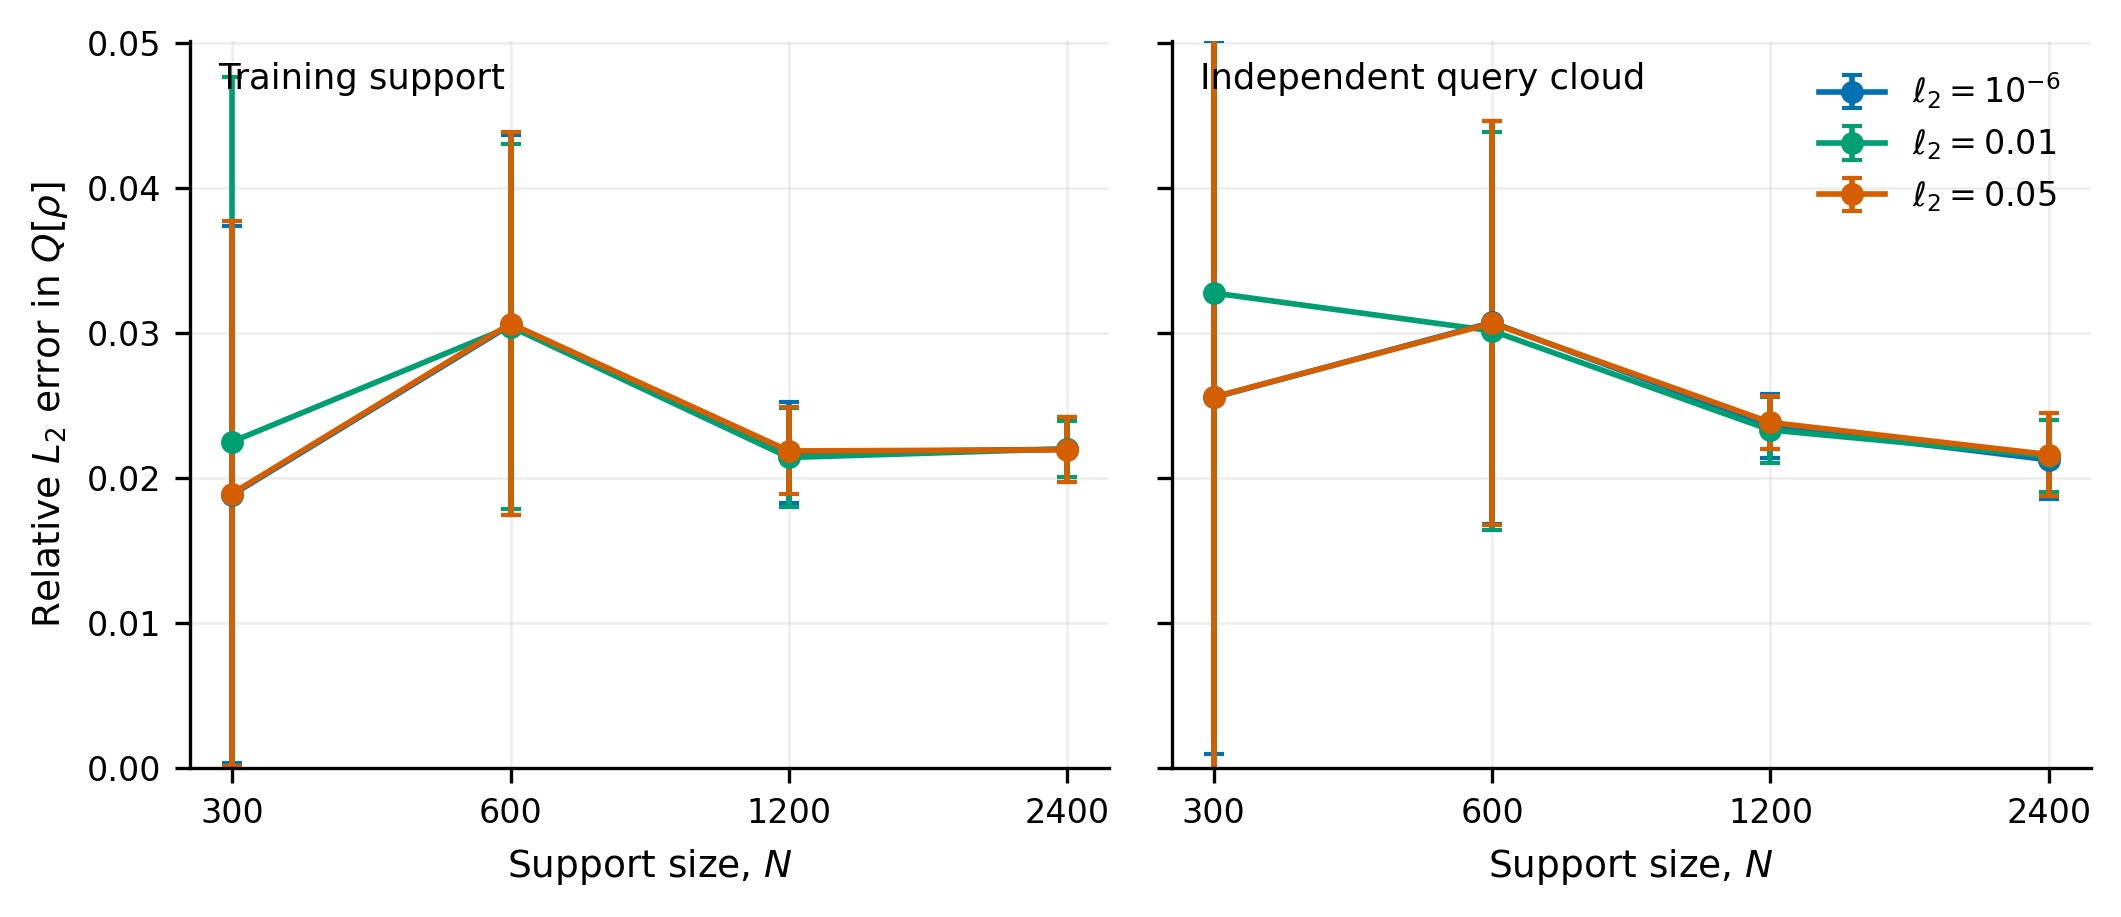
\includegraphics[width=0.96\textwidth]{../final_reviewer_closure/figures/manufactured_operator_regularization.png}
\caption{Manufactured relative \(L_2\) error in the excess action \(Q[\rho]\)
on the training cloud and on an independent query cloud. Points are means
over seeds 123, 124, and 125; bars are sample standard deviations. The three
regularization policies use paired training and query clouds at each cloud
size. The error remains nonzero and nonmonotone, so neither cloud enlargement
nor changing \(\ell_2\) from \(10^{-6}\) to the pilot \(0.01\) or production
\(0.05\) policy establishes a monotone error decrease under independent-cloud
enlargement.}
\label{fig:manufactured-operator-regularization}
\end{figure}

\section{Physical SEO image and identical-cloud reconstruction}
\label{sec:results-projection}

The two-state physical SEO image has four real bath-dependent coefficient
fields. Table~\ref{tab:seo-projection-physics} measures the relative distance
of the fitted product density from this image using 20 bath anchors and 400
mapping probes. The projection is diagnosed but not imposed. Across the
reported snapshots and initial momenta, the mean leakage spans approximately
0.221--0.977, which is too large to regard the propagated surrogate as a small
perturbation within the physical SEO subspace. This is a representation
diagnostic, not a TDSE or QCLE error.

The identical-cloud comparison in
Table~\ref{tab:identical-cloud-reconstruction} addresses a narrower question:
can the GP reproduce a KDE density when both estimators use the same PBME
snapshot, weights, bandwidth, normalization, and evaluation grid? The maximum
\(E_1\) values are well below the declared \(0.02\) criterion. This positive
control confirms accurate same-cloud value reconstruction, but it does not
test derivatives, the SEO constraint, or time propagation.

\begingroup
\scriptsize
\setlength{\tabcolsep}{3.5pt}
\begin{longtable}{l r r r r}
\caption{Relative $L_2$ distance from the four-field physical SEO image at three collision-time snapshots.  The entries are mean $\pm$ sample standard deviation over four independently propagated clouds; projection is diagnosed by least squares but is not imposed during propagation.}\label{tab:seo-projection-physics}\\
\toprule
Method & $P_{\rm init}$ & $t/t_c$ & Mean leakage & Largest local leakage \\
\midrule
\endfirsthead
\multicolumn{5}{l}{\tablename\ \thetable\ (continued)}\\
\toprule
Method & $P_{\rm init}$ & $t/t_c$ & Mean leakage & Largest local leakage \\
\midrule
\endhead
\midrule
\multicolumn{5}{r}{Continued on next page}\\
\endfoot
\bottomrule
\endlastfoot
PBME & 20 & $0$ & $0.222\pm 0.00155$ & $0.256$ \\
PBME & 20 & $1$ & $0.803\pm 0.0769$ & $0.993$ \\
PBME & 20 & $2$ & $0.32\pm 0.0339$ & $0.777$ \\
PBME & 100 & $0$ & $0.222\pm 0.00155$ & $0.256$ \\
PBME & 100 & $1$ & $0.962\pm 0.00312$ & $0.998$ \\
PBME & 100 & $2$ & $0.959\pm 0.0109$ & $0.997$ \\
MIDPOINT & 20 & $0$ & $0.222\pm 0.00155$ & $0.256$ \\
MIDPOINT & 20 & $1$ & $0.864\pm 0.0338$ & $0.998$ \\
MIDPOINT & 20 & $2$ & $0.626\pm 0.163$ & $0.99$ \\
MIDPOINT & 100 & $0$ & $0.222\pm 0.00155$ & $0.256$ \\
MIDPOINT & 100 & $1$ & $0.968\pm 0.00653$ & $0.999$ \\
MIDPOINT & 100 & $2$ & $0.967\pm 0.00671$ & $0.998$ \\
\end{longtable}
\endgroup

\begingroup
\scriptsize
\setlength{\tabcolsep}{3.5pt}
\begin{longtable}{r r r r r L{0.27\textwidth}}
\caption{Identical-cloud KDE/GP reconstruction control.  Both estimators use the same PBME snapshot, weights, bandwidth convention, normalization, and evaluation grid.  The declared criterion concerns $E_1$ only and does not test derivatives or propagation.}\label{tab:identical-cloud-reconstruction}\\
\toprule
$P_{\rm init}$ & Cases & $\max E_1$ & $\max E_2$ & $\max E_\infty$ & Declared reconstruction criterion \\
\midrule
\endfirsthead
\multicolumn{6}{l}{\tablename\ \thetable\ (continued)}\\
\toprule
$P_{\rm init}$ & Cases & $\max E_1$ & $\max E_2$ & $\max E_\infty$ & Declared reconstruction criterion \\
\midrule
\endhead
\midrule
\multicolumn{6}{r}{Continued on next page}\\
\endfoot
\bottomrule
\endlastfoot
20 & 12 & $0.00118$ & $4.24\times10^{-4}$ & $5.88\times10^{-4}$ & $E_1\leq 0.02$ (criterion met) \\
100 & 12 & $0.00155$ & $5.16\times10^{-4}$ & $9.28\times10^{-4}$ & $E_1\leq 0.02$ (criterion met) \\
\end{longtable}
\endgroup

The nonzero initial value in Table~\ref{tab:seo-projection-physics} requires
explicit interpretation. At \(t=0\) the analytic initial density is the
occupied-state SEO profile multiplied by a smooth bath factor, so it lies
exactly in the four-field image and its residual under the same projector
vanishes identically in exact arithmetic. The reported initial leakage of
approximately 0.222 is therefore a property of the fitted finite surrogate as
evaluated by this diagnostic, not of the physical initial target: the
20-anchor/400-probe evaluation samples mapping directions that the focused
initial cloud does not constrain, where the fitted product density is
determined by the Gaussian-process extension and the safe-profile floor
rather than by data. PBME and MIDPOINT report identical initial values
because both branches share the same initial fit before any excess source is
applied. The present calculations do not apportion this initial residual
among the Gaussian-process extension, the floor regularization, and the
finite anchor/probe sampling; the subsequent growth of the leakage along the
propagation, not the initial offset, carries the propagation-relevant
conclusion.

The four-seed snapshot summary in
Figure~\ref{fig:seo-projection-leakage-verified} shows that the leakage is not
a small local residual confined to one calculation.
\begin{figure}[tbp]
\centering
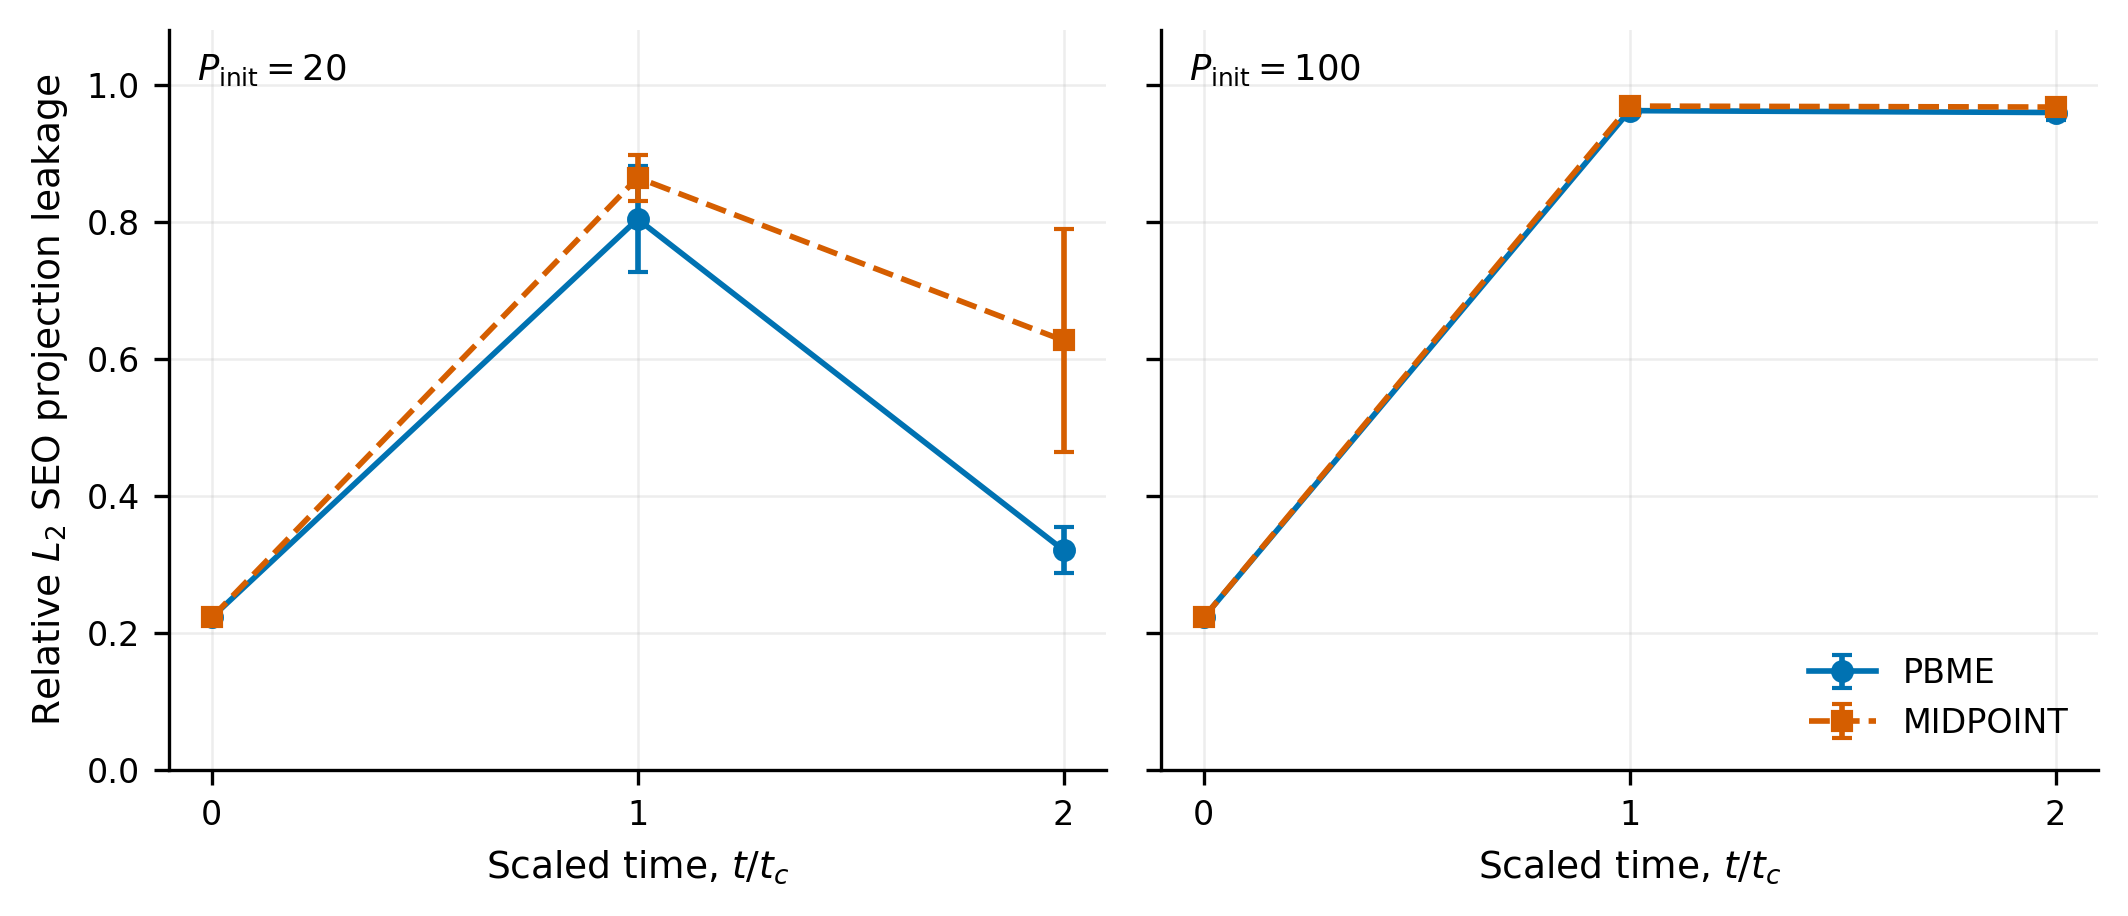
\includegraphics[width=0.96\textwidth]{../final_reviewer_closure/figures/seo_projection_leakage_verified.png}
\caption{Diagnostic SEO projection leakage at \(t/t_c=0,1,2\). Each point is
the mean over four independent propagation seeds and each bar is the sample
standard deviation. The plotted quantity is the relative \(L_2\) residual
\(\lVert y-Bc\rVert_2/\max(\lVert y\rVert_2,10^{-30})\) from a four-field
least-squares SEO projection using 20 bath anchors and 400 mapping probes.
Projection is diagnosed but not enforced, and this quantity is not a physical
TDSE or QCLE error.}
\label{fig:seo-projection-leakage-verified}
\end{figure}

\section{Time-step refinement}
\label{sec:results-timestep}

Table~\ref{tab:timestep-refinement-physics} compares
\(\Delta t=0.5,0.25,0.125\) on common physical times using linear
interpolation without extrapolation. Both successive time-normalized
differences must first exceed
\(\tau_{\rm noise}=10^{-12}+10^{-12}\max_k\operatorname{RMS}(O_k)\).
Rows below that floor are labelled roundoff- or saturation-limited; rows with
nondecreasing successive differences are labelled nonmonotone. For MIDPOINT,
both differences must additionally exceed the pooled dispersion over four
independently sampled clouds. The 128 run/observable rows comprise 15
noise-limited rejections, 102 seed-variability rejections, three nonpositive
orders, and eight positive orders. The latter do not repair the simultaneous
failures in replication and raw conservation, so the formal order of the
midpoint formula is not promoted to a demonstrated order of the full
moving-cloud dynamics.

\begin{landscape}
\begingroup
\scriptsize
\setlength{\tabcolsep}{3.5pt}
\begin{longtable}{l r l r r r r r L{0.20\textwidth}}
\caption{Time-step sensitivity of endpoint observables. Values and time-normalized successive differences are averages over seeds 11, 29, 47, and 73 after interpolation to common physical times without extrapolation. Both differences must exceed the declared absolute-plus-relative floor $\tau_{\rm noise}=10^{-12}+10^{-12}\max_k\operatorname{RMS}(O_k)$ before an order is interpreted; MIDPOINT additionally requires both differences to exceed pooled independent-seed dispersion.}\label{tab:timestep-refinement-physics}\\
\toprule
Method & $P_{\rm init}$ & Observable & $\langle y_{0.5}\rangle$ & $\langle y_{0.25}\rangle$ & $\langle y_{0.125}\rangle$ & $\langle D_{12}\rangle$ & $\langle D_{23}\rangle$ & Interpretation \\
\midrule
\endfirsthead
\multicolumn{9}{l}{\tablename\ \thetable\ (continued)}\\
\toprule
Method & $P_{\rm init}$ & Observable & $\langle y_{0.5}\rangle$ & $\langle y_{0.25}\rangle$ & $\langle y_{0.125}\rangle$ & $\langle D_{12}\rangle$ & $\langle D_{23}\rangle$ & Interpretation \\
\midrule
\endhead
\midrule
\multicolumn{9}{r}{Continued on next page}\\
\endfoot
\bottomrule
\endlastfoot
PBME & 20 & $\rho_{11}^{\mathrm{SN}}$ & $0.964$ & $0.964$ & $0.964$ & $7.02\times10^{-7}$ & $1.75\times10^{-7}$ & step-size signal is not resolved above seed spread \\
PBME & 20 & $\rho_{22}^{\mathrm{SN}}$ & $0.0357$ & $0.0357$ & $0.0357$ & $7.02\times10^{-7}$ & $1.75\times10^{-7}$ & step-size signal is not resolved above seed spread \\
PBME & 20 & electronic trace & $1$ & $1$ & $1$ & $2.90\times10^{-13}$ & $5.91\times10^{-13}$ & roundoff- or saturation-limited; order not interpreted \\
PBME & 20 & energy & $0.1$ & $0.1$ & $0.1$ & $4.93\times10^{-9}$ & $1.23\times10^{-9}$ & step-size signal is not resolved above seed spread \\
PBME & 20 & $\langle R\rangle$ & $15.3$ & $15.3$ & $15.3$ & $1.48\times10^{-6}$ & $3.69\times10^{-7}$ & step-size signal is not resolved above seed spread \\
PBME & 20 & $\langle P\rangle$ & $19.8$ & $19.8$ & $19.8$ & $3.50\times10^{-6}$ & $8.74\times10^{-7}$ & step-size signal is not resolved above seed spread \\
PBME & 20 & $\operatorname{var}(R)$ & $2.31$ & $2.31$ & $2.31$ & $4.89\times10^{-7}$ & $1.22\times10^{-7}$ & step-size signal is not resolved above seed spread \\
PBME & 20 & $\operatorname{var}(P)$ & $1.66$ & $1.66$ & $1.66$ & $3.00\times10^{-6}$ & $7.49\times10^{-7}$ & step-size signal is not resolved above seed spread \\
PBME & 100 & $\rho_{11}^{\mathrm{SN}}$ & $0.137$ & $0.137$ & $0.137$ & $6.74\times10^{-6}$ & $1.69\times10^{-6}$ & step-size signal is not resolved above seed spread \\
PBME & 100 & $\rho_{22}^{\mathrm{SN}}$ & $0.863$ & $0.863$ & $0.863$ & $6.74\times10^{-6}$ & $1.69\times10^{-6}$ & step-size signal is not resolved above seed spread \\
PBME & 100 & electronic trace & $1$ & $1$ & $1$ & $5.64\times10^{-14}$ & $1.16\times10^{-13}$ & roundoff- or saturation-limited; order not interpreted \\
PBME & 100 & energy & $2.5$ & $2.5$ & $2.5$ & $5.98\times10^{-8}$ & $1.50\times10^{-8}$ & step-size signal is not resolved above seed spread \\
PBME & 100 & $\langle R\rangle$ & $14.9$ & $14.9$ & $14.9$ & $3.94\times10^{-7}$ & $9.85\times10^{-8}$ & step-size signal is not resolved above seed spread \\
PBME & 100 & $\langle P\rangle$ & $99.1$ & $99.1$ & $99.1$ & $6.82\times10^{-6}$ & $1.70\times10^{-6}$ & step-size signal is not resolved above seed spread \\
PBME & 100 & $\operatorname{var}(R)$ & $0.985$ & $0.985$ & $0.985$ & $1.81\times10^{-7}$ & $4.51\times10^{-8}$ & step-size signal is not resolved above seed spread \\
PBME & 100 & $\operatorname{var}(P)$ & $0.444$ & $0.444$ & $0.444$ & $7.48\times10^{-6}$ & $1.87\times10^{-6}$ & step-size signal is not resolved above seed spread \\
MIDPOINT & 20 & $\rho_{11}^{\mathrm{SN}}$ & $1.18$ & $1.31$ & $0.818$ & $0.525$ & $0.422$ & contracting signal resolved above noise and seed spread \\
MIDPOINT & 20 & $\rho_{22}^{\mathrm{SN}}$ & $-0.18$ & $-0.312$ & $0.182$ & $0.525$ & $0.422$ & contracting signal resolved above noise and seed spread \\
MIDPOINT & 20 & electronic trace & $1$ & $1$ & $1$ & $1.45\times10^{-12}$ & $1.68\times10^{-12}$ & roundoff- or saturation-limited; order not interpreted \\
MIDPOINT & 20 & energy & $0.107$ & $0.126$ & $0.0937$ & $0.0317$ & $0.0232$ & step-size signal is not resolved above seed spread \\
MIDPOINT & 20 & $\langle R\rangle$ & $16.6$ & $14.3$ & $13.9$ & $2.38$ & $2.21$ & step-size signal is not resolved above seed spread \\
MIDPOINT & 20 & $\langle P\rangle$ & $21.5$ & $24.2$ & $18.5$ & $4.91$ & $3.96$ & contracting signal resolved above noise and seed spread \\
MIDPOINT & 20 & $\operatorname{var}(R)$ & $-1.52\times10^{3}$ & $-5.07$ & $-13.1$ & $503$ & $8.38$ & step-size signal is not resolved above seed spread \\
MIDPOINT & 20 & $\operatorname{var}(P)$ & $-2.67\times10^{3}$ & $11.4$ & $-13.4$ & $1.94\times10^{3}$ & $82.5$ & step-size signal is not resolved above seed spread \\
MIDPOINT & 100 & $\rho_{11}^{\mathrm{SN}}$ & $-0.201$ & $-0.198$ & $-0.18$ & $5.74$ & $5.82$ & nonmonotone step-size response \\
MIDPOINT & 100 & $\rho_{22}^{\mathrm{SN}}$ & $1.2$ & $1.2$ & $1.18$ & $5.74$ & $5.82$ & nonmonotone step-size response \\
MIDPOINT & 100 & electronic trace & $1$ & $1$ & $1$ & $7.61\times10^{-13}$ & $1.44\times10^{-12}$ & roundoff- or saturation-limited; order not interpreted \\
MIDPOINT & 100 & energy & $2.5$ & $2.53$ & $2.52$ & $0.704$ & $0.722$ & nonmonotone step-size response \\
MIDPOINT & 100 & $\langle R\rangle$ & $12.8$ & $12.5$ & $12.6$ & $14.5$ & $12.4$ & step-size signal is not resolved above seed spread \\
MIDPOINT & 100 & $\langle P\rangle$ & $98.8$ & $99.4$ & $99.2$ & $18.2$ & $18$ & step-size signal is not resolved above seed spread \\
MIDPOINT & 100 & $\operatorname{var}(R)$ & $-1.02\times10^{44}$ & $-1.27\times10^{43}$ & $-6.88\times10^{45}$ & $2.95\times10^{43}$ & $2.01\times10^{45}$ & nonmonotone step-size response \\
MIDPOINT & 100 & $\operatorname{var}(P)$ & $-5.96\times10^{45}$ & $-9.50\times10^{44}$ & $-4.79\times10^{47}$ & $3.06\times10^{45}$ & $2.38\times10^{47}$ & nonmonotone step-size response \\
\end{longtable}
\endgroup
\end{landscape}

\section{Independent-cloud enlargement and four-seed replication}
\label{sec:results-support-replication}

The cloud-size study in Table~\ref{tab:independent-cloud-size} compares
\(N=500,1000,2000\) using three independently sampled clouds at each size.
These clouds are not nested; the results therefore measure sensitivity to
enlarging a stochastic representation rather than deterministic convergence.
Several MIDPOINT changes remain comparable to, or larger than, the seed
dispersion, while PBME is generally much more stable.

Table~\ref{tab:four-seed-replication-physics} makes that contrast explicit at
\(N=1000\) and \(\Delta t=0.25\). For the endpoint \(\rho_{11}^{\mathrm{SN}}\) estimator, the
PBME sample standard deviation is 0.00788 at initial momentum 20 and 0.0154 at
initial momentum 100; the corresponding MIDPOINT values are 0.795 and 0.956.
The MIDPOINT mean and interval can also extend outside the physical population
range \([0,1]\). Four seeds provide a sensitive instability diagnostic but
not a precise uncertainty distribution, so the intervals are interpreted
descriptively.

\begin{landscape}
\begingroup
\scriptsize
\setlength{\tabcolsep}{3.5pt}
\begin{longtable}{l r l r r r L{0.24\textwidth}}
\caption{Sensitivity to enlarging independently sampled trajectory clouds.  Each entry is mean $\pm$ sample standard deviation over seeds 11, 29, and 47.  Because the clouds are independently sampled rather than nested, this is a stochastic cloud-size test, not a deterministic convergence order.}\label{tab:independent-cloud-size}\\
\toprule
Method & $P_{\rm init}$ & Observable & $N=500$ & $N=1000$ & $N=2000$ & Interpretation \\
\midrule
\endfirsthead
\multicolumn{7}{l}{\tablename\ \thetable\ (continued)}\\
\toprule
Method & $P_{\rm init}$ & Observable & $N=500$ & $N=1000$ & $N=2000$ & Interpretation \\
\midrule
\endhead
\midrule
\multicolumn{7}{r}{Continued on next page}\\
\endfoot
\bottomrule
\endlastfoot
PBME & 20 & $\rho_{11}^{\mathrm{SN}}$ & $0.963\pm 0.0109$ & $0.964\pm 0.00965$ & $0.953\pm 0.00151$ & cloud-size change exceeds seed spread \\
PBME & 20 & $\rho_{22}^{\mathrm{SN}}$ & $0.0369\pm 0.0109$ & $0.0356\pm 0.00965$ & $0.0472\pm 0.00151$ & cloud-size change exceeds seed spread \\
PBME & 20 & electronic trace & $1\pm 7.72\times10^{-15}$ & $1\pm 3.67\times10^{-15}$ & $1\pm 1.12\times10^{-15}$ & cloud-size change exceeds seed spread \\
PBME & 20 & energy & $0.0999\pm 1.94\times10^{-4}$ & $0.1\pm 9.32\times10^{-5}$ & $0.1\pm 9.57\times10^{-5}$ & change remains within seed spread \\
PBME & 20 & $\langle R\rangle$ & $15.3\pm 0.033$ & $15.3\pm 0.0236$ & $15.3\pm 0.0264$ & cloud-size change exceeds seed spread \\
PBME & 20 & $\langle P\rangle$ & $19.8\pm 0.0466$ & $19.8\pm 0.0583$ & $19.7\pm 0.013$ & cloud-size change exceeds seed spread \\
PBME & 20 & $\operatorname{var}(R)$ & $2.18\pm 0.124$ & $2.37\pm 0.133$ & $2.31\pm 0.0335$ & change remains within seed spread \\
PBME & 20 & $\operatorname{var}(P)$ & $1.46\pm 0.0285$ & $1.7\pm 0.097$ & $1.7\pm 0.0634$ & cloud-size change exceeds seed spread \\
PBME & 100 & $\rho_{11}^{\mathrm{SN}}$ & $0.137\pm 0.00679$ & $0.135\pm 0.0178$ & $0.143\pm 0.006$ & change remains within seed spread \\
PBME & 100 & $\rho_{22}^{\mathrm{SN}}$ & $0.863\pm 0.00679$ & $0.865\pm 0.0178$ & $0.857\pm 0.006$ & change remains within seed spread \\
PBME & 100 & electronic trace & $1\pm 9.02\times10^{-16}$ & $1\pm 1.78\times10^{-15}$ & $1\pm 3.51\times10^{-16}$ & change remains within seed spread \\
PBME & 100 & energy & $2.5\pm 9.52\times10^{-4}$ & $2.5\pm 4.71\times10^{-4}$ & $2.5\pm 4.84\times10^{-4}$ & change remains within seed spread \\
PBME & 100 & $\langle R\rangle$ & $14.9\pm 0.0205$ & $14.9\pm 0.0249$ & $14.9\pm 0.0124$ & change remains within seed spread \\
PBME & 100 & $\langle P\rangle$ & $99.1\pm 0.0226$ & $99.1\pm 0.0247$ & $99.1\pm 0.00766$ & cloud-size change exceeds seed spread \\
PBME & 100 & $\operatorname{var}(R)$ & $0.979\pm 0.0751$ & $0.986\pm 0.054$ & $1\pm 0.0299$ & change remains within seed spread \\
PBME & 100 & $\operatorname{var}(P)$ & $0.426\pm 0.0187$ & $0.447\pm 0.0117$ & $0.46\pm 0.00392$ & cloud-size change exceeds seed spread \\
MIDPOINT & 20 & $\rho_{11}^{\mathrm{SN}}$ & $1.08\pm 0.0635$ & $0.916\pm 0.0672$ & $0.951\pm 0.0744$ & cloud-size change exceeds seed spread \\
MIDPOINT & 20 & $\rho_{22}^{\mathrm{SN}}$ & $-0.079\pm 0.0635$ & $0.0841\pm 0.0672$ & $0.0485\pm 0.0744$ & cloud-size change exceeds seed spread \\
MIDPOINT & 20 & electronic trace & $1\pm 6.46\times10^{-13}$ & $1\pm 6.09\times10^{-13}$ & $1\pm 7.07\times10^{-13}$ & change remains within seed spread \\
MIDPOINT & 20 & energy & $0.101\pm 0.0214$ & $0.0994\pm 0.0167$ & $0.0934\pm 0.0207$ & change remains within seed spread \\
MIDPOINT & 20 & $\langle R\rangle$ & $16.9\pm 0.989$ & $14.9\pm 2$ & $14.5\pm 2.24$ & change remains within seed spread \\
MIDPOINT & 20 & $\langle P\rangle$ & $20.5\pm 1.93$ & $19.5\pm 1.73$ & $19\pm 1.75$ & change remains within seed spread \\
MIDPOINT & 20 & $\operatorname{var}(R)$ & $-1.31\times10^{3}\pm 262$ & $-9.5\pm 52.5$ & $-1.94\times10^{8}\pm 3.31\times10^{8}$ & change remains within seed spread \\
MIDPOINT & 20 & $\operatorname{var}(P)$ & $-1.94\times10^{3}\pm 571$ & $-6.33\pm 85.3$ & $-3.87\times10^{8}\pm 6.63\times10^{8}$ & change remains within seed spread \\
MIDPOINT & 100 & $\rho_{11}^{\mathrm{SN}}$ & $0.923\pm 1.01$ & $-0.46\pm 0.98$ & $-0.297\pm 0.842$ & change remains within seed spread \\
MIDPOINT & 100 & $\rho_{22}^{\mathrm{SN}}$ & $0.0775\pm 1.01$ & $1.46\pm 0.98$ & $1.3\pm 0.842$ & change remains within seed spread \\
MIDPOINT & 100 & electronic trace & $1\pm 1.39\times10^{-13}$ & $1\pm 7.76\times10^{-14}$ & $1\pm 3.65\times10^{-14}$ & change remains within seed spread \\
MIDPOINT & 100 & energy & $2.41\pm 0.0692$ & $2.53\pm 0.107$ & $2.5\pm 0.05$ & change remains within seed spread \\
MIDPOINT & 100 & $\langle R\rangle$ & $12.4\pm 3.43$ & $12.5\pm 0.978$ & $12.6\pm 1.27$ & change remains within seed spread \\
MIDPOINT & 100 & $\langle P\rangle$ & $98.2\pm 0.412$ & $99.2\pm 1.28$ & $98.7\pm 1.29$ & change remains within seed spread \\
MIDPOINT & 100 & $\operatorname{var}(R)$ & $-1.47\times10^{19}\pm 2.54\times10^{19}$ & $-1.69\times10^{43}\pm 2.56\times10^{43}$ & $-4.76\times10^{94}\pm 8.25\times10^{94}$ & change remains within seed spread \\
MIDPOINT & 100 & $\operatorname{var}(P)$ & $-8.89\times10^{20}\pm 1.53\times10^{21}$ & $-1.27\times10^{45}\pm 1.96\times10^{45}$ & $-2.43\times10^{96}\pm 4.20\times10^{96}$ & change remains within seed spread \\
\end{longtable}
\endgroup
\end{landscape}

\begin{landscape}
\begingroup
\scriptsize
\setlength{\tabcolsep}{3.5pt}
\begin{longtable}{l r l r r r r}
\caption{Four-seed endpoint replication at $N=1000$ and $\Delta t=0.25$.  The interval is a two-sided Student-$t$ interval with three degrees of freedom and is interpreted as a small-sample sensitivity measure, not as strong uncertainty calibration.}\label{tab:four-seed-replication-physics}\\
\toprule
Method & $P_{\rm init}$ & Observable & Mean & Sample SD & 95\% interval & Max. spread \\
\midrule
\endfirsthead
\multicolumn{7}{l}{\tablename\ \thetable\ (continued)}\\
\toprule
Method & $P_{\rm init}$ & Observable & Mean & Sample SD & 95\% interval & Max. spread \\
\midrule
\endhead
\midrule
\multicolumn{7}{r}{Continued on next page}\\
\endfoot
\bottomrule
\endlastfoot
PBME & 20 & $\rho_{11}^{\mathrm{SN}}$ & $0.964$ & $0.00788$ & $[0.952,0.977]$ & $0.019$ \\
PBME & 20 & $\rho_{22}^{\mathrm{SN}}$ & $0.0357$ & $0.00788$ & $[0.0231,0.0482]$ & $0.019$ \\
PBME & 20 & electronic trace & $1$ & $3.08\times10^{-15}$ & $[1,1]$ & $7.33\times10^{-15}$ \\
PBME & 20 & energy & $0.1$ & $8.18\times10^{-5}$ & $[0.0999,0.1]$ & $1.79\times10^{-4}$ \\
PBME & 20 & $\langle R\rangle$ & $15.3$ & $0.0227$ & $[15.3,15.4]$ & $0.0458$ \\
PBME & 20 & $\langle P\rangle$ & $19.8$ & $0.0476$ & $[19.7,19.9]$ & $0.111$ \\
PBME & 20 & $\operatorname{var}(R)$ & $2.31$ & $0.163$ & $[2.05,2.57]$ & $0.357$ \\
PBME & 20 & $\operatorname{var}(P)$ & $1.66$ & $0.118$ & $[1.47,1.85]$ & $0.281$ \\
PBME & 100 & $\rho_{11}^{\mathrm{SN}}$ & $0.137$ & $0.0154$ & $[0.113,0.162]$ & $0.0333$ \\
PBME & 100 & $\rho_{22}^{\mathrm{SN}}$ & $0.863$ & $0.0154$ & $[0.838,0.887]$ & $0.0333$ \\
PBME & 100 & electronic trace & $1$ & $1.46\times10^{-15}$ & $[1,1]$ & $3.33\times10^{-15}$ \\
PBME & 100 & energy & $2.5$ & $4.13\times10^{-4}$ & $[2.5,2.5]$ & $9.07\times10^{-4}$ \\
PBME & 100 & $\langle R\rangle$ & $14.9$ & $0.0271$ & $[14.9,14.9]$ & $0.0543$ \\
PBME & 100 & $\langle P\rangle$ & $99.1$ & $0.0203$ & $[99.1,99.2]$ & $0.0461$ \\
PBME & 100 & $\operatorname{var}(R)$ & $0.985$ & $0.0441$ & $[0.915,1.06]$ & $0.0944$ \\
PBME & 100 & $\operatorname{var}(P)$ & $0.444$ & $0.0116$ & $[0.426,0.463]$ & $0.021$ \\
MIDPOINT & 20 & $\rho_{11}^{\mathrm{SN}}$ & $1.31$ & $0.795$ & $[0.0475,2.58]$ & $1.65$ \\
MIDPOINT & 20 & $\rho_{22}^{\mathrm{SN}}$ & $-0.312$ & $0.795$ & $[-1.58,0.952]$ & $1.65$ \\
MIDPOINT & 20 & electronic trace & $1$ & $2.52\times10^{-12}$ & $[1,1]$ & $5.34\times10^{-12}$ \\
MIDPOINT & 20 & energy & $0.126$ & $0.0557$ & $[0.0378,0.215]$ & $0.122$ \\
MIDPOINT & 20 & $\langle R\rangle$ & $14.3$ & $1.98$ & $[11.2,17.5]$ & $4.08$ \\
MIDPOINT & 20 & $\langle P\rangle$ & $24.2$ & $9.49$ & $[9.11,39.3]$ & $20.4$ \\
MIDPOINT & 20 & $\operatorname{var}(R)$ & $-5.07$ & $43.8$ & $[-74.8,64.6]$ & $104$ \\
MIDPOINT & 20 & $\operatorname{var}(P)$ & $11.4$ & $78.1$ & $[-113,136]$ & $170$ \\
MIDPOINT & 100 & $\rho_{11}^{\mathrm{SN}}$ & $-0.198$ & $0.956$ & $[-1.72,1.32]$ & $2.07$ \\
MIDPOINT & 100 & $\rho_{22}^{\mathrm{SN}}$ & $1.2$ & $0.956$ & $[-0.324,2.72]$ & $2.07$ \\
MIDPOINT & 100 & electronic trace & $1$ & $6.41\times10^{-14}$ & $[1,1]$ & $1.41\times10^{-13}$ \\
MIDPOINT & 100 & energy & $2.53$ & $0.0879$ & $[2.39,2.67]$ & $0.207$ \\
MIDPOINT & 100 & $\langle R\rangle$ & $12.5$ & $0.799$ & $[11.2,13.8]$ & $1.92$ \\
MIDPOINT & 100 & $\langle P\rangle$ & $99.4$ & $1.1$ & $[97.6,101]$ & $2.22$ \\
MIDPOINT & 100 & $\operatorname{var}(R)$ & $-1.27\times10^{43}$ & $2.25\times10^{43}$ & $[-4.85\times10^{43},2.31\times10^{43}]$ & $4.63\times10^{43}$ \\
MIDPOINT & 100 & $\operatorname{var}(P)$ & $-9.50\times10^{44}$ & $1.72\times10^{45}$ & $[-3.69\times10^{45},1.79\times10^{45}]$ & $3.52\times10^{45}$ \\
\end{longtable}
\endgroup
\end{landscape}

Figure~\ref{fig:replication-raw-conservation} places the seed instability and
the associated raw conservation failure on the same footing.
\begin{figure}[tbp]
\centering
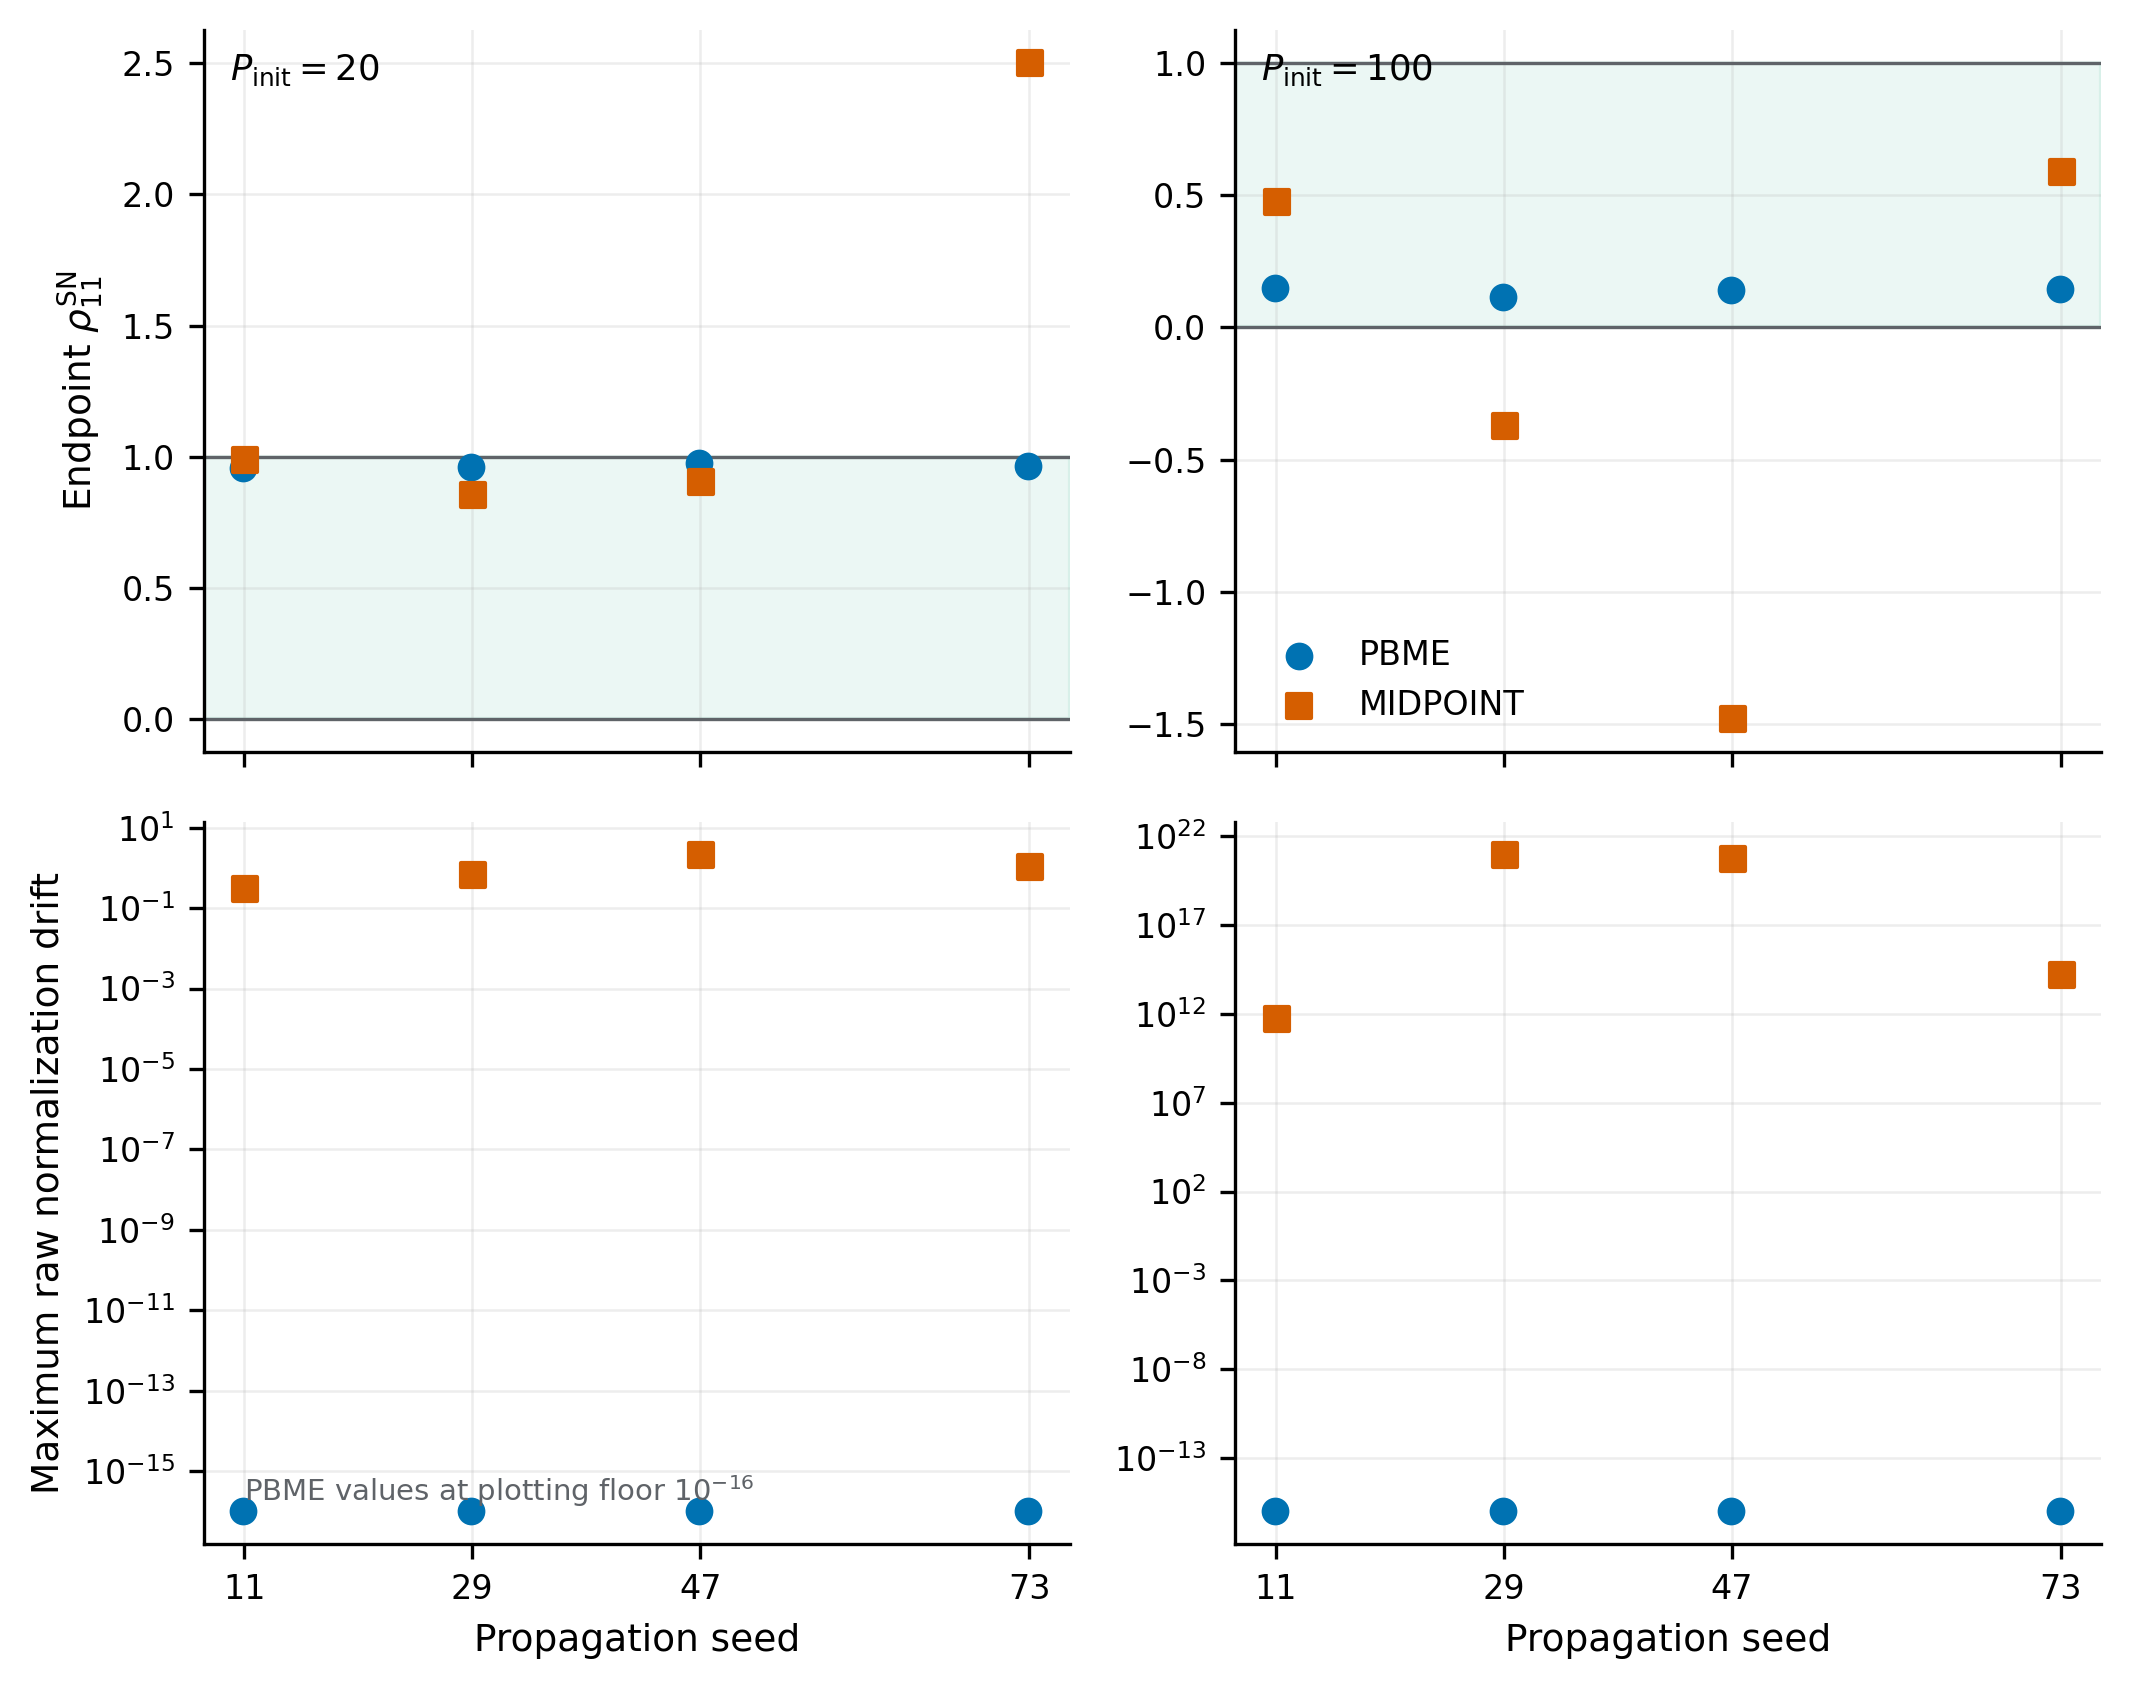
\includegraphics[width=0.91\textwidth]{../final_reviewer_closure/figures/replication_and_raw_conservation.png}
\caption{Four-seed replication and raw pre-normalization conservation for the
canonical \(N=1000\), \(\Delta t=0.25\) calculations. The upper panels show
the endpoint \(\rho_{11}^{\mathrm{SN}}\) estimator; the shaded band marks the physical interval
\([0,1]\). The lower panels show the maximum absolute drift of the raw
normalization. Exact PBME zeros are displayed at \(10^{-16}\) only to make
them visible on the logarithmic axis. The seed count is four, not the number
of trajectories, and the plot supplies a descriptive sensitivity comparison
rather than strong uncertainty calibration.}
\label{fig:replication-raw-conservation}
\end{figure}

\section{Raw conservation and signed-label tail sensitivity}
\label{sec:results-conservation-tail}

The population and density curves shown elsewhere can be normalized for visual
comparison, but that operation removes the very integral whose conservation
must be tested. Table~\ref{tab:raw-conservation-physics} therefore reports the
normalization, electronic trace, and energy before any such rescaling. PBME
keeps the raw normalization constant in these calculations and its trace and
energy drifts remain small. MIDPOINT shows large and strongly seed-dependent
drifts: even in the canonical four-seed set the largest normalization drift
reaches \(8.69\times10^{20}\), and across the tested refinement/cloud-size
calculations it reaches \(7.35\times10^{46}\). A unit-normalized display curve
cannot be used as evidence against this failure.

The signed-label diagnostic in Table~\ref{tab:signed-label-tail-physics}
quantifies the conditioning of the ratio \(y_i(t)/y_i^0\). At zero threshold,
the largest absolute ratio reaches \(7.61\times10^{23}\) and the signed
effective sample size falls as low as 0.0247. The first nonzero threshold,
however, already removes about \(10^{-3}\) of the absolute physical mass,
which is larger than the predeclared negligible-mass allowance of \(10^{-6}\).
Thus there is no nontrivial negligible-mass plateau. The signed estimator is
demonstrably ill-conditioned, but these calculations do not isolate a
vanishing-initial-label tail as its unique cause.

\begingroup
\scriptsize
\setlength{\tabcolsep}{3.5pt}
\begin{longtable}{l r l r r r}
\caption{Raw pre-normalization conservation diagnostics for the canonical four-seed calculations ($N=1000$, $\Delta t=0.25$).  The largest drift is the maximum over both time and seeds; the RMS column is averaged over seeds.  These raw quantities are evaluated before any display normalization.}\label{tab:raw-conservation-physics}\\
\toprule
Method & $P_{\rm init}$ & Quantity & Largest $|\Delta|$ & Mean RMS drift & Endpoint-drift range \\
\midrule
\endfirsthead
\multicolumn{6}{l}{\tablename\ \thetable\ (continued)}\\
\toprule
Method & $P_{\rm init}$ & Quantity & Largest $|\Delta|$ & Mean RMS drift & Endpoint-drift range \\
\midrule
\endhead
\midrule
\multicolumn{6}{r}{Continued on next page}\\
\endfoot
\bottomrule
\endlastfoot
PBME & 20 & normalization & $0$ & $0$ & $[0,0]$ \\
PBME & 20 & trace & $1.17\times10^{-12}$ & $6.08\times10^{-13}$ & $[1.16\times10^{-12},1.17\times10^{-12}]$ \\
PBME & 20 & energy & $6.38\times10^{-9}$ & $1.64\times10^{-9}$ & $[1.45\times10^{-13},4.38\times10^{-13}]$ \\
PBME & 100 & normalization & $0$ & $0$ & $[0,0]$ \\
PBME & 100 & trace & $2.28\times10^{-13}$ & $1.18\times10^{-13}$ & $[2.25\times10^{-13},2.28\times10^{-13}]$ \\
PBME & 100 & energy & $8.02\times10^{-8}$ & $1.99\times10^{-8}$ & $[-9.10\times10^{-13},-3.81\times10^{-13}]$ \\
MIDPOINT & 20 & normalization & $2.07$ & $0.353$ & $[-0.938,0.174]$ \\
MIDPOINT & 20 & trace & $2.07$ & $0.353$ & $[-0.938,0.174]$ \\
MIDPOINT & 20 & energy & $0.244$ & $0.0387$ & $[-0.0871,0.0383]$ \\
MIDPOINT & 100 & normalization & $8.69\times10^{20}$ & $9.95\times10^{19}$ & $[-1.66\times10^{20},5.94\times10^{20}]$ \\
MIDPOINT & 100 & trace & $8.69\times10^{20}$ & $9.95\times10^{19}$ & $[-1.66\times10^{20},5.94\times10^{20}]$ \\
MIDPOINT & 100 & energy & $2.22\times10^{21}$ & $2.56\times10^{20}$ & $[-4.36\times10^{20},1.52\times10^{21}]$ \\
\end{longtable}
\endgroup

\begin{landscape}
\begingroup
\scriptsize
\setlength{\tabcolsep}{3.5pt}
\begin{longtable}{l r r r r r r r r}
\caption{Signed-label conditioning and tail sensitivity.  The first nonzero threshold excludes about $10^{-3}$ of the absolute physical mass, already above the predeclared negligible-mass allowance $10^{-6}$.  Consequently no nontrivial negligible-mass plateau exists from which to attribute the instability uniquely to a vanishing-$|y_i^0|$ tail.}\label{tab:signed-label-tail-physics}\\
\toprule
Method & $P_{\rm init}$ & Seed & $\max|y/y^0|$ & $N_{\rm eff}^{\rm signed}$ & $N_{\rm eff}^{\rm abs}$ & Raw norm & First $\eta$ & Excluded mass \\
\midrule
\endfirsthead
\multicolumn{9}{l}{\tablename\ \thetable\ (continued)}\\
\toprule
Method & $P_{\rm init}$ & Seed & $\max|y/y^0|$ & $N_{\rm eff}^{\rm signed}$ & $N_{\rm eff}^{\rm abs}$ & Raw norm & First $\eta$ & Excluded mass \\
\midrule
\endhead
\midrule
\multicolumn{9}{r}{Continued on next page}\\
\endfoot
\bottomrule
\endlastfoot
MIDPOINT & 20 & 11 & $333$ & $4.07$ & $46$ & $1$ & $0.001$ & $1.00\times10^{-3}$ \\
MIDPOINT & 20 & 29 & $176$ & $3.97$ & $92.6$ & $0.439$ & $0.001$ & $1.00\times10^{-3}$ \\
MIDPOINT & 20 & 47 & $999$ & $0.669$ & $32.3$ & $1.17$ & $0.001$ & $1.00\times10^{-3}$ \\
MIDPOINT & 20 & 73 & $256$ & $0.0247$ & $73.5$ & $0.0621$ & $0.01$ & $0.008$ \\
MIDPOINT & 100 & 11 & $2.55\times10^{14}$ & $0.961$ & $27.6$ & $-4.75\times10^{11}$ & $0.001$ & $1.00\times10^{-3}$ \\
MIDPOINT & 100 & 29 & $7.61\times10^{23}$ & $0.5$ & $16.4$ & $5.94\times10^{20}$ & $0.001$ & $1.00\times10^{-3}$ \\
MIDPOINT & 100 & 47 & $3.38\times10^{23}$ & $0.204$ & $12.2$ & $-1.66\times10^{20}$ & $0.001$ & $1.00\times10^{-3}$ \\
MIDPOINT & 100 & 73 & $4.83\times10^{16}$ & $0.478$ & $70.4$ & $-9.29\times10^{13}$ & $0.01$ & $0.008$ \\
PBME & 20 & 11 & $1$ & $1.00\times10^{3}$ & $1.00\times10^{3}$ & $1$ & $0.001$ & $1.00\times10^{-3}$ \\
PBME & 20 & 29 & $1$ & $1.00\times10^{3}$ & $1.00\times10^{3}$ & $1$ & $0.001$ & $1.00\times10^{-3}$ \\
PBME & 20 & 47 & $1$ & $1.00\times10^{3}$ & $1.00\times10^{3}$ & $1$ & $0.001$ & $1.00\times10^{-3}$ \\
PBME & 20 & 73 & $1$ & $1.00\times10^{3}$ & $1.00\times10^{3}$ & $1$ & $0.01$ & $0.008$ \\
PBME & 100 & 11 & $1$ & $1.00\times10^{3}$ & $1.00\times10^{3}$ & $1$ & $0.001$ & $1.00\times10^{-3}$ \\
PBME & 100 & 29 & $1$ & $1.00\times10^{3}$ & $1.00\times10^{3}$ & $1$ & $0.001$ & $1.00\times10^{-3}$ \\
PBME & 100 & 47 & $1$ & $1.00\times10^{3}$ & $1.00\times10^{3}$ & $1$ & $0.001$ & $1.00\times10^{-3}$ \\
PBME & 100 & 73 & $1$ & $1.00\times10^{3}$ & $1.00\times10^{3}$ & $1$ & $0.01$ & $0.008$ \\
\end{longtable}
\endgroup
\end{landscape}

Figure~\ref{fig:initial-label-tail-sensitivity} shows the paired
initial-label distributions and the threshold sweep behind
Table~\ref{tab:signed-label-tail-physics}.
\begin{figure}[tbp]
\centering
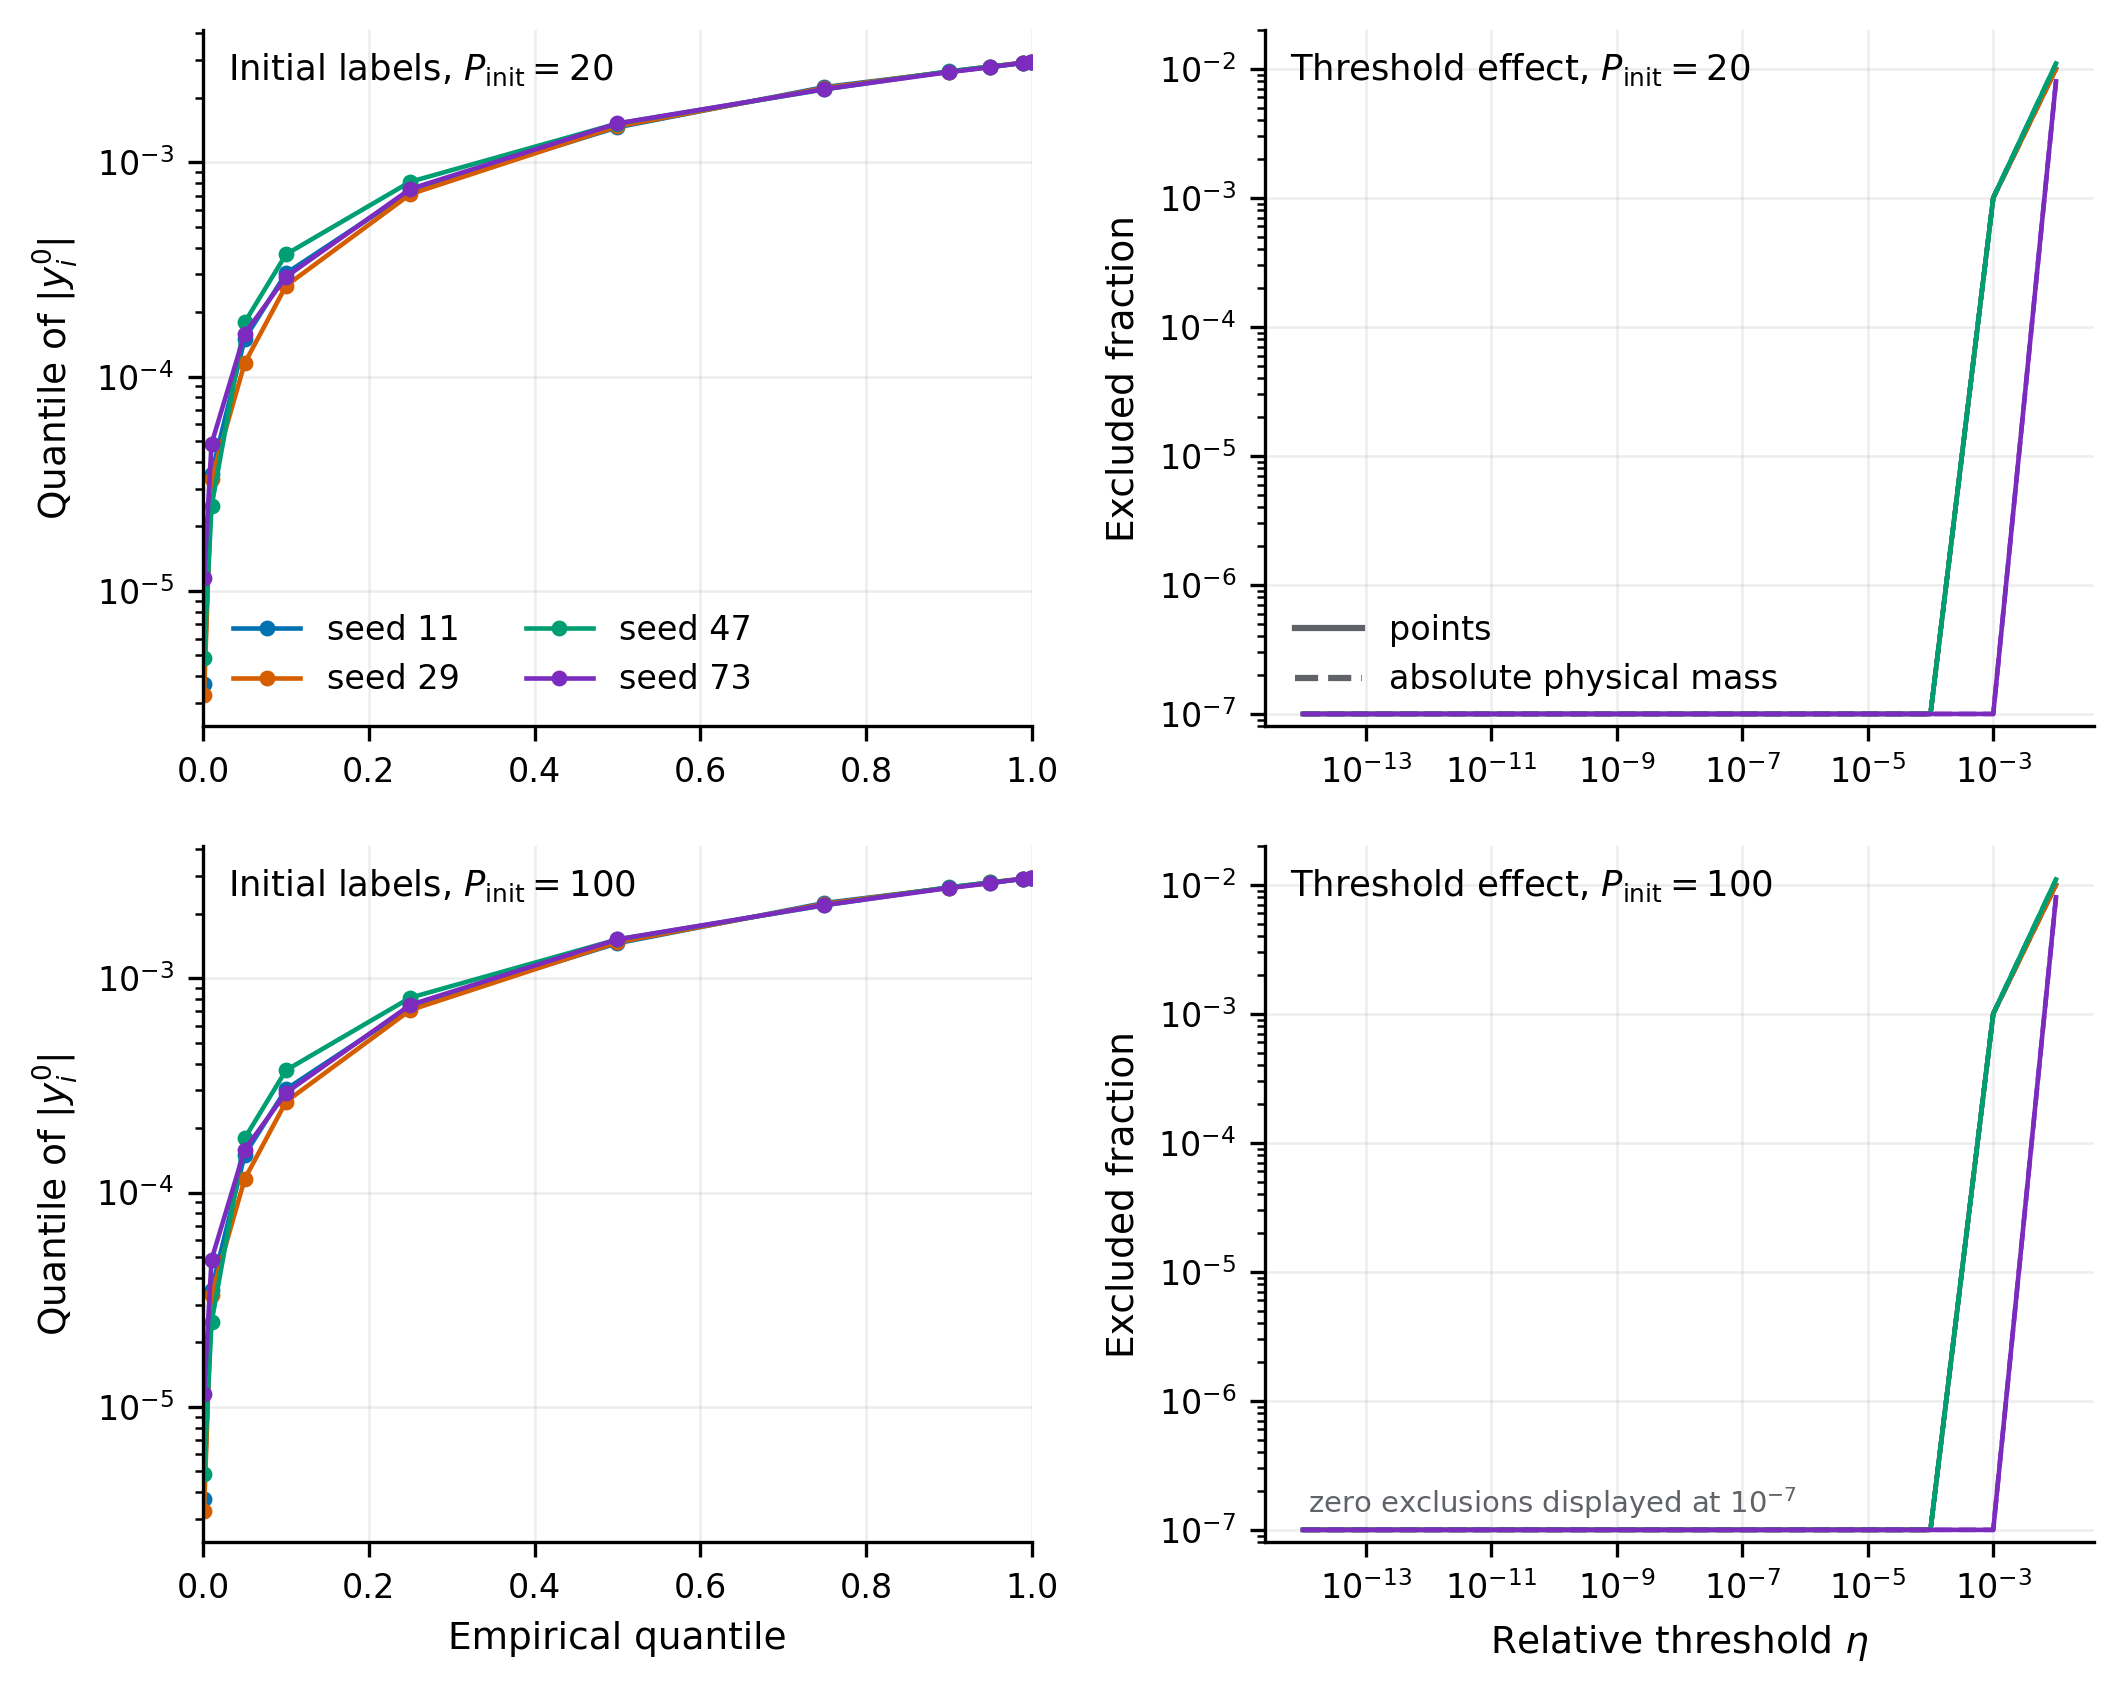
\includegraphics[width=0.96\textwidth]{../final_reviewer_closure/figures/initial_label_tail_sensitivity.png}
\caption{Initial-label tail sensitivity for all eight paired
\(P_{\rm init}\)/seed cases. The quantile panel reports the \(|y_i^0|\)
distribution on the grid \(q=0.001,\ldots,0.999\); the threshold panels use
the PBME copy of the method-identical inclusion masks at every positive
threshold \(\eta\). Solid lines are excluded point fractions and dashed
lines are excluded absolute physical-mass fractions; exact zeros are plotted
at \(10^{-7}\) only for logarithmic display and do not alter any reported
error. The first nonzero threshold already excludes about \(10^{-3}\) of the
absolute physical mass, exceeding the predeclared \(10^{-6}\) allowance, so
no negligible-mass plateau exists.}
\label{fig:initial-label-tail-sensitivity}
\end{figure}

\section{TDSE and grid-QCLE numerical controls}
\label{sec:results-reference-controls}

TDSE is model-exact only within the displayed domain, time step, periodic FFT
convention, edge-mass, normalization, and reflected-momentum controls. Grid
QCLE is a numerical solution of the approximate QCLE equation. Its separate
temporal and phase-space-grid studies report three levels and both successive
differences for each observable. The exact domains and discretizations are
collected in Table~\ref{tab:reference-discretizations}, while
Tables~\ref{tab:tdse-reference-refinement} and
\ref{tab:qcle-reference-refinement} give the observable-level comparisons.

The maximum TDSE boundary probability in the outer spatial bands is
\(1.22\times10^{-24}\), and the maximum negative-momentum probability for the
high-momentum case is \(6.09\times10^{-27}\), both negligible on the declared
scale. For grid QCLE, the largest physical marginal fractions in the outer
5\% bands are \(2.51\times10^{-4}\) in \(R\) and
\(5.92\times10^{-4}\) in \(P\), below the \(10^{-3}\) criterion. An auxiliary
phase-space \(|W|\)-weighted edge diagnostic can reach \(7.94\times10^{-2}\)
because the Wigner density is sign-indefinite and exhibits numerical ringing;
it is retained as a ringing diagnostic and is not substituted for the physical
marginal boundary mass. The CFL ratios also remain below unity. For
\(P_{\rm init}=100\), the nominal TDSE grid levels all resolve to the required
8192-point grid; that case therefore establishes boundary adequacy and
numerical repeatability on the chosen grid, but not an independent spatial
convergence rate.

The expected temporal scaling is approximately second order for the TDSE
split-operator calculation and approximately fourth order for the grid-QCLE
classical RK4 calculation. Spatial or phase-space-grid behaviour is assessed
separately and is not assigned either temporal order. An observed order is
reported only when both successive differences exceed the same declared
absolute-plus-relative noise floor, decrease monotonically, and give
\(0<p\leq6\); more rapid contractions are retained as nonasymptotic rather
than promoted as convergence evidence.

% Auto-generated by reviewer_final_closure.py.
% Source CSV: D:\PhD-Project\GP_RKHS_MINT\GP_RKHS_MINT\Tully_models\GP_MInt_QCLE_Reviewer_Ready_Pipeline_v4\output\fixed_pipeline\final_reviewer_closure\reference_settings_by_method_and_momentum.csv
\begin{landscape}
\begin{table}[p]
\centering
\caption{Reference settings split by equation, initial momentum, and refinement mode.}\label{tab:reference-discretizations}
\resizebox{\linewidth}{!}{%
\begin{tabular}{@{}rrrrrrrrrrr@{}}
\toprule
Method & $P_{\mathrm{init}}$ & Mode & $t_{\mathrm{final}}$ & $\Delta t$ ladder & Grid ladder & $R$ domains & $P$ domains & Finest edge fraction & Finest CFL & Interpretation \\
\midrule
TDSE & 20 & grid & 3000 & 0.05/0.05/0.05 & 2048/4096/8192 & [-40,45.958]/[-40,45.979]/[-40,45.9895] & --- & 6.164956e-25 & --- & three-level refinement \\
TDSE & 20 & time & 3000 & 0.2/0.1/0.05 & 8192/8192/8192 & [-40,45.9895]/[-40,45.9895]/[-40,45.9895] & --- & 1.223884e-24 & --- & three-level refinement \\
TDSE & 100 & grid & 600 & 0.05/0.05/0.05 & 8192/8192/8192 & [-40,45.9895]/[-40,45.9895]/[-40,45.9895] & --- & 4.825683e-26 & --- & boundary adequacy/repeatability; no independent grid order \\
TDSE & 100 & time & 600 & 0.2/0.1/0.05 & 8192/8192/8192 & [-40,45.9895]/[-40,45.9895]/[-40,45.9895] & --- & 4.825683e-26 & --- & three-level refinement \\
grid QCLE & 20 & grid & 3000 & 0.5/0.5/0.5 & 48x64/96x128/192x256 & [-30,30]/[-30,30]/[-30,30] & [-35,35]/[-35,35]/[-35,35] & 5.915682e-04 & 0.09195161 & three-level refinement \\
grid QCLE & 20 & time & 3000 & 2/1/0.5 & 192x256/192x256/192x256 & [-30,30]/[-30,30]/[-30,30] & [-35,35]/[-35,35]/[-35,35] & 5.915682e-04 & 0.09195161 & three-level refinement \\
grid QCLE & 100 & grid & 600 & 0.5/0.5/0.5 & 48x32/96x64/192x128 & [-30,30]/[-30,30]/[-30,30] & [80,120]/[80,120]/[80,120] & 1.697013e-07 & 0.1066453 & three-level refinement \\
grid QCLE & 100 & time & 600 & 2/1/0.5 & 192x128/192x128/192x128 & [-30,30]/[-30,30]/[-30,30] & [80,120]/[80,120]/[80,120] & 2.152345e-07 & 0.1066453 & three-level refinement \\
\bottomrule
\end{tabular}%
}
\par\vspace{3pt}
\begin{minipage}{0.97\linewidth}\footnotesize Slash-separated entries are coarse/fine/finer. For grid QCLE, the reported edge value is the larger of the finest-grid physical R and P marginal edge fractions. The sign-indefinite phase-space absolute-W ringing diagnostic is not substituted for this boundary-mass control. The dimensionless CFL entry is Delta t/Delta t\_max, where Delta t\_max is the minimum of the RK4 imaginary-axis bound 2.828 divided by the spectral advection, force, and electronic-frequency scales; values below one satisfy this declared linear-stability check.\end{minipage}
\end{table}
\end{landscape}


\begin{landscape}
\begingroup
\scriptsize
\setlength{\tabcolsep}{3.5pt}
\begin{longtable}{l r l r r r r r L{0.18\textwidth}}
\caption{Three-level TDSE reference study. Time and spatial/grid refinement are performed separately. $\delta_{12}$ and $\delta_{23}$ are successive absolute differences. Both must exceed $\tau_{\rm noise}=10^{-12}+10^{-12}\max_k|O_k|$; nonmonotone rows and values above the plausibility bound $p\le6$ are retained but not interpreted as convergence orders.}\label{tab:tdse-reference-refinement}\\
\toprule
Refinement & $P_{\rm init}$ & Observable & Level 1 & Level 2 & Level 3 & $\delta_{12}$ & $\delta_{23}$ & Interpretation \\
\midrule
\endfirsthead
\multicolumn{9}{l}{\tablename\ \thetable\ (continued)}\\
\toprule
Refinement & $P_{\rm init}$ & Observable & Level 1 & Level 2 & Level 3 & $\delta_{12}$ & $\delta_{23}$ & Interpretation \\
\midrule
\endhead
\midrule
\multicolumn{9}{r}{Continued on next page}\\
\endfoot
\bottomrule
\endlastfoot
time & 20 & $\rho_{11}^{\mathrm{SN}}$ & $0.952$ & $0.952$ & $0.952$ & $1.20\times10^{-7}$ & $3.00\times10^{-8}$ & $p=2$ \\
time & 20 & $\rho_{22}^{\mathrm{SN}}$ & $0.0481$ & $0.0481$ & $0.0481$ & $1.20\times10^{-7}$ & $3.00\times10^{-8}$ & $p=2$ \\
time & 20 & electronic trace & $1$ & $1$ & $1$ & $4.14\times10^{-12}$ & $6.22\times10^{-12}$ & non-monotone or unresolved \\
time & 20 & energy & $0.1$ & $0.1$ & $0.1$ & $4.15\times10^{-13}$ & $6.20\times10^{-13}$ & roundoff- or saturation-limited; order not interpreted \\
time & 20 & $\langle R\rangle$ & $15.3$ & $15.3$ & $15.3$ & $4.91\times10^{-7}$ & $1.23\times10^{-7}$ & $p=2$ \\
time & 20 & $\langle P\rangle$ & $19.7$ & $19.7$ & $19.7$ & $7.10\times10^{-7}$ & $1.78\times10^{-7}$ & $p=2$ \\
time & 20 & $\operatorname{var}(R)$ & $2.41$ & $2.41$ & $2.41$ & $1.85\times10^{-6}$ & $4.64\times10^{-7}$ & $p=2$ \\
time & 20 & $\operatorname{var}(P)$ & $2.07$ & $2.07$ & $2.07$ & $4.00\times10^{-6}$ & $1.00\times10^{-6}$ & $p=2$ \\
time & 100 & $\rho_{11}^{\mathrm{SN}}$ & $0.143$ & $0.143$ & $0.143$ & $1.57\times10^{-6}$ & $3.92\times10^{-7}$ & $p=2$ \\
time & 100 & $\rho_{22}^{\mathrm{SN}}$ & $0.857$ & $0.857$ & $0.857$ & $1.57\times10^{-6}$ & $3.92\times10^{-7}$ & $p=2$ \\
time & 100 & electronic trace & $1$ & $1$ & $1$ & $1.22\times10^{-12}$ & $2.20\times10^{-12}$ & roundoff- or saturation-limited; order not interpreted \\
time & 100 & energy & $2.5$ & $2.5$ & $2.5$ & $2.86\times10^{-12}$ & $5.44\times10^{-12}$ & roundoff- or saturation-limited; order not interpreted \\
time & 100 & $\langle R\rangle$ & $14.9$ & $14.9$ & $14.9$ & $1.81\times10^{-7}$ & $4.54\times10^{-8}$ & $p=2$ \\
time & 100 & $\langle P\rangle$ & $99.1$ & $99.1$ & $99.1$ & $1.58\times10^{-6}$ & $3.94\times10^{-7}$ & $p=2$ \\
time & 100 & $\operatorname{var}(R)$ & $1.01$ & $1.01$ & $1.01$ & $4.65\times10^{-8}$ & $1.16\times10^{-8}$ & $p=2$ \\
time & 100 & $\operatorname{var}(P)$ & $0.376$ & $0.376$ & $0.376$ & $1.12\times10^{-6}$ & $2.79\times10^{-7}$ & $p=2$ \\
grid & 20 & $\rho_{11}^{\mathrm{SN}}$ & $0.952$ & $0.952$ & $0.952$ & $4.59\times10^{-12}$ & $1.80\times10^{-12}$ & roundoff- or saturation-limited; order not interpreted \\
grid & 20 & $\rho_{22}^{\mathrm{SN}}$ & $0.0481$ & $0.0481$ & $0.0481$ & $4.48\times10^{-14}$ & $2.12\times10^{-14}$ & roundoff- or saturation-limited; order not interpreted \\
grid & 20 & electronic trace & $1$ & $1$ & $1$ & $4.64\times10^{-12}$ & $1.77\times10^{-12}$ & roundoff- or saturation-limited; order not interpreted \\
grid & 20 & energy & $0.1$ & $0.1$ & $0.1$ & $4.68\times10^{-13}$ & $1.72\times10^{-13}$ & roundoff- or saturation-limited; order not interpreted \\
grid & 20 & $\langle R\rangle$ & $15.3$ & $15.3$ & $15.3$ & $1.79\times10^{-12}$ & $3.77\times10^{-13}$ & roundoff- or saturation-limited; order not interpreted \\
grid & 20 & $\langle P\rangle$ & $19.7$ & $19.7$ & $19.7$ & $1.43\times10^{-12}$ & $1.17\times10^{-13}$ & roundoff- or saturation-limited; order not interpreted \\
grid & 20 & $\operatorname{var}(R)$ & $2.41$ & $2.41$ & $2.41$ & $2.10\times10^{-12}$ & $3.15\times10^{-12}$ & roundoff- or saturation-limited; order not interpreted \\
grid & 20 & $\operatorname{var}(P)$ & $2.07$ & $2.07$ & $2.07$ & $5.91\times10^{-12}$ & $3.58\times10^{-12}$ & $p=0.723$ \\
grid & 100 & $\rho_{11}^{\mathrm{SN}}$ & $0.143$ & $0.143$ & $0.143$ & $0$ & $0$ & roundoff- or saturation-limited; order not interpreted \\
grid & 100 & $\rho_{22}^{\mathrm{SN}}$ & $0.857$ & $0.857$ & $0.857$ & $0$ & $0$ & roundoff- or saturation-limited; order not interpreted \\
grid & 100 & electronic trace & $1$ & $1$ & $1$ & $0$ & $0$ & roundoff- or saturation-limited; order not interpreted \\
grid & 100 & energy & $2.5$ & $2.5$ & $2.5$ & $0$ & $0$ & roundoff- or saturation-limited; order not interpreted \\
grid & 100 & $\langle R\rangle$ & $14.9$ & $14.9$ & $14.9$ & $0$ & $0$ & roundoff- or saturation-limited; order not interpreted \\
grid & 100 & $\langle P\rangle$ & $99.1$ & $99.1$ & $99.1$ & $0$ & $0$ & roundoff- or saturation-limited; order not interpreted \\
grid & 100 & $\operatorname{var}(R)$ & $1.01$ & $1.01$ & $1.01$ & $0$ & $0$ & roundoff- or saturation-limited; order not interpreted \\
grid & 100 & $\operatorname{var}(P)$ & $0.376$ & $0.376$ & $0.376$ & $0$ & $0$ & roundoff- or saturation-limited; order not interpreted \\
\end{longtable}
\endgroup
\end{landscape}

\begin{landscape}
\begingroup
\scriptsize
\setlength{\tabcolsep}{3.5pt}
\begin{longtable}{l r l r r r r r L{0.18\textwidth}}
\caption{Three-level grid QCLE reference study. Time and spatial/grid refinement are performed separately. $\delta_{12}$ and $\delta_{23}$ are successive absolute differences. Both must exceed $\tau_{\rm noise}=10^{-12}+10^{-12}\max_k|O_k|$; nonmonotone rows and values above the plausibility bound $p\le6$ are retained but not interpreted as convergence orders.}\label{tab:qcle-reference-refinement}\\
\toprule
Refinement & $P_{\rm init}$ & Observable & Level 1 & Level 2 & Level 3 & $\delta_{12}$ & $\delta_{23}$ & Interpretation \\
\midrule
\endfirsthead
\multicolumn{9}{l}{\tablename\ \thetable\ (continued)}\\
\toprule
Refinement & $P_{\rm init}$ & Observable & Level 1 & Level 2 & Level 3 & $\delta_{12}$ & $\delta_{23}$ & Interpretation \\
\midrule
\endhead
\midrule
\multicolumn{9}{r}{Continued on next page}\\
\endfoot
\bottomrule
\endlastfoot
time & 20 & $\rho_{11}^{\mathrm{SN}}$ & $0.948$ & $0.948$ & $0.948$ & $1.27\times10^{-10}$ & $7.86\times10^{-12}$ & $p=4.01$ \\
time & 20 & $\rho_{22}^{\mathrm{SN}}$ & $0.0518$ & $0.0518$ & $0.0518$ & $1.27\times10^{-10}$ & $7.86\times10^{-12}$ & $p=4.01$ \\
time & 20 & electronic trace & $1$ & $1$ & $1$ & $6.66\times10^{-16}$ & $4.44\times10^{-16}$ & roundoff- or saturation-limited; order not interpreted \\
time & 20 & energy & $0.1$ & $0.1$ & $0.1$ & $2.08\times10^{-16}$ & $1.39\times10^{-17}$ & roundoff- or saturation-limited; order not interpreted \\
time & 20 & $\langle R\rangle$ & $15.3$ & $15.3$ & $15.3$ & $1.43\times10^{-10}$ & $9.07\times10^{-12}$ & roundoff- or saturation-limited; order not interpreted \\
time & 20 & $\langle P\rangle$ & $19.7$ & $19.7$ & $19.7$ & $1.21\times10^{-11}$ & $1.13\times10^{-12}$ & roundoff- or saturation-limited; order not interpreted \\
time & 20 & $\operatorname{var}(R)$ & $2.14$ & $2.14$ & $2.14$ & $4.36\times10^{-9}$ & $2.76\times10^{-10}$ & $p=3.98$ \\
time & 20 & $\operatorname{var}(P)$ & $1.05$ & $1.05$ & $1.05$ & $1.46\times10^{-9}$ & $1.09\times10^{-10}$ & $p=3.75$ \\
time & 100 & $\rho_{11}^{\mathrm{SN}}$ & $0.143$ & $0.143$ & $0.143$ & $1.68\times10^{-10}$ & $9.50\times10^{-12}$ & $p=4.14$ \\
time & 100 & $\rho_{22}^{\mathrm{SN}}$ & $0.857$ & $0.857$ & $0.857$ & $1.68\times10^{-10}$ & $9.50\times10^{-12}$ & $p=4.14$ \\
time & 100 & electronic trace & $1$ & $1$ & $1$ & $0$ & $2.22\times10^{-16}$ & roundoff- or saturation-limited; order not interpreted \\
time & 100 & energy & $2.5$ & $2.5$ & $2.5$ & $2.22\times10^{-15}$ & $4.44\times10^{-16}$ & roundoff- or saturation-limited; order not interpreted \\
time & 100 & $\langle R\rangle$ & $14.9$ & $14.9$ & $14.9$ & $1.78\times10^{-12}$ & $1.05\times10^{-13}$ & roundoff- or saturation-limited; order not interpreted \\
time & 100 & $\langle P\rangle$ & $99.1$ & $99.1$ & $99.1$ & $1.96\times10^{-10}$ & $1.22\times10^{-11}$ & roundoff- or saturation-limited; order not interpreted \\
time & 100 & $\operatorname{var}(R)$ & $1.01$ & $1.01$ & $1.01$ & $1.42\times10^{-11}$ & $7.67\times10^{-13}$ & roundoff- or saturation-limited; order not interpreted \\
time & 100 & $\operatorname{var}(P)$ & $0.382$ & $0.382$ & $0.382$ & $1.62\times10^{-10}$ & $7.28\times10^{-12}$ & $p=4.48$ \\
grid & 20 & $\rho_{11}^{\mathrm{SN}}$ & $0.412$ & $1.05$ & $0.948$ & $0.638$ & $0.102$ & $p=2.64$ \\
grid & 20 & $\rho_{22}^{\mathrm{SN}}$ & $0.595$ & $-0.0502$ & $0.0518$ & $0.645$ & $0.102$ & $p=2.66$ \\
grid & 20 & electronic trace & $1.01$ & $1$ & $1$ & $0.00719$ & $1.23\times10^{-7}$ & rapid contraction; order not interpreted (not demonstrably asymptotic) \\
grid & 20 & energy & $0.101$ & $0.1$ & $0.1$ & $0.00129$ & $3.76\times10^{-5}$ & $p=5.1$ \\
grid & 20 & $\langle R\rangle$ & $14.2$ & $15.5$ & $15.3$ & $1.37$ & $0.242$ & $p=2.5$ \\
grid & 20 & $\langle P\rangle$ & $14.7$ & $20.1$ & $19.7$ & $5.33$ & $0.37$ & $p=3.85$ \\
grid & 20 & $\operatorname{var}(R)$ & $10.7$ & $1.26$ & $2.14$ & $9.47$ & $0.874$ & $p=3.44$ \\
grid & 20 & $\operatorname{var}(P)$ & $37$ & $0.451$ & $1.05$ & $36.6$ & $0.595$ & $p=5.94$ \\
grid & 100 & $\rho_{11}^{\mathrm{SN}}$ & $0.107$ & $0.143$ & $0.143$ & $0.0361$ & $6.54\times10^{-5}$ & rapid contraction; order not interpreted (not demonstrably asymptotic) \\
grid & 100 & $\rho_{22}^{\mathrm{SN}}$ & $0.808$ & $0.857$ & $0.857$ & $0.0488$ & $5.89\times10^{-5}$ & rapid contraction; order not interpreted (not demonstrably asymptotic) \\
grid & 100 & electronic trace & $0.915$ & $1$ & $1$ & $0.085$ & $6.52\times10^{-6}$ & rapid contraction; order not interpreted (not demonstrably asymptotic) \\
grid & 100 & energy & $2.29$ & $2.5$ & $2.5$ & $0.213$ & $1.56\times10^{-5}$ & rapid contraction; order not interpreted (not demonstrably asymptotic) \\
grid & 100 & $\langle R\rangle$ & $14.9$ & $14.9$ & $14.9$ & $0.00136$ & $1.71\times10^{-4}$ & $p=2.98$ \\
grid & 100 & $\langle P\rangle$ & $99.1$ & $99.1$ & $99.1$ & $0.0337$ & $2.61\times10^{-5}$ & rapid contraction; order not interpreted (not demonstrably asymptotic) \\
grid & 100 & $\operatorname{var}(R)$ & $0.954$ & $1.01$ & $1.01$ & $0.0529$ & $5.98\times10^{-4}$ & rapid contraction; order not interpreted (not demonstrably asymptotic) \\
grid & 100 & $\operatorname{var}(P)$ & $0.51$ & $0.381$ & $0.382$ & $0.129$ & $0.00106$ & rapid contraction; order not interpreted (not demonstrably asymptotic) \\
\end{longtable}
\endgroup
\end{landscape}

\section{PBME versus MIDPOINT against common references}
\label{sec:results-physical-comparison}

Each paired difference is
\(E_{\mathrm{MIDPOINT,ref}}-E_{\mathrm{PBME,ref}}\), so a negative value
favours MIDPOINT for that particular metric. Isolated negative differences do
not establish systematic improvement. Table~\ref{tab:paired-physical-errors}
reports the paired mean and Student-\(t\) interval for raw and unit-mass density
errors and for the principal time-dependent observables. Several intervals
include zero, and resolved comparisons are not consistently in favour of
MIDPOINT. More fundamentally, a physical success claim also requires
seed-stable dynamics, raw conservation, and controlled discretization
sensitivity. Those conditions are not met, so systematic improvement over
PBME is not demonstrated.

\begin{landscape}
\begingroup
\scriptsize
\setlength{\tabcolsep}{3.5pt}
\begin{longtable}{l r l l r r L{0.23\textwidth}}
\caption{Paired physical-error comparison against common references.  The reported difference is $\Delta E=E_{\mathrm{MIDPOINT}}-E_{\mathrm{PBME}}$ over the same four independent seeds; negative values favour MIDPOINT for that metric.  Intervals are paired Student-$t$ 95\% intervals with three degrees of freedom.  Raw and unit-mass density errors are distinguished so that shape normalization cannot hide normalization error.}\label{tab:paired-physical-errors}\\
\toprule
Reference & $P_{\rm init}$ & Quantity & Error measure & $\langle\Delta E\rangle$ & 95\% interval & Interpretation \\
\midrule
\endfirsthead
\multicolumn{7}{l}{\tablename\ \thetable\ (continued)}\\
\toprule
Reference & $P_{\rm init}$ & Quantity & Error measure & $\langle\Delta E\rangle$ & 95\% interval & Interpretation \\
\midrule
\endhead
\midrule
\multicolumn{7}{r}{Continued on next page}\\
\endfoot
\bottomrule
\endlastfoot
QCLE & 20 & $R$--$P$ density & raw $E_1$ & $0.506$ & $[-0.297,1.31]$ & interval includes zero \\
QCLE & 20 & $R$--$P$ density & unit-mass shape $E_1$ & $2.61$ & $[-3.87,9.09]$ & interval includes zero \\
QCLE & 20 & $\rho_{11}^{\mathrm{SN}}$ & time-series RMS error & $0.378$ & $[-0.435,1.19]$ & interval includes zero \\
QCLE & 20 & $\rho_{22}^{\mathrm{SN}}$ & time-series RMS error & $0.378$ & $[-0.435,1.19]$ & interval includes zero \\
QCLE & 20 & $\langle P\rangle$ & time-series RMS error & $3.69$ & $[-5.32,12.7]$ & interval includes zero \\
QCLE & 20 & $\langle R\rangle$ & time-series RMS error & $1.97$ & $[-2.22,6.16]$ & interval includes zero \\
QCLE & 100 & $R$--$P$ density & raw $E_1$ & $4.89\times10^{20}$ & $[-5.69\times10^{20},1.55\times10^{21}]$ & interval includes zero \\
QCLE & 100 & $R$--$P$ density & unit-mass shape $E_1$ & $3.07$ & $[2.62,3.52]$ & PBME smaller for this metric \\
QCLE & 100 & $\rho_{11}^{\mathrm{SN}}$ & time-series RMS error & $51.4$ & $[-103,206]$ & interval includes zero \\
QCLE & 100 & $\rho_{22}^{\mathrm{SN}}$ & time-series RMS error & $51.4$ & $[-103,206]$ & interval includes zero \\
QCLE & 100 & $\langle P\rangle$ & time-series RMS error & $144$ & $[-296,584]$ & interval includes zero \\
QCLE & 100 & $\langle R\rangle$ & time-series RMS error & $108$ & $[-225,441]$ & interval includes zero \\
TDSE & 20 & $\rho_{11}^{\mathrm{SN}}$ & time-series RMS error & $0.38$ & $[-0.431,1.19]$ & interval includes zero \\
TDSE & 20 & $\rho_{22}^{\mathrm{SN}}$ & time-series RMS error & $0.38$ & $[-0.431,1.19]$ & interval includes zero \\
TDSE & 20 & $\langle P\rangle$ & time-series RMS error & $3.7$ & $[-5.3,12.7]$ & interval includes zero \\
TDSE & 20 & $\langle R\rangle$ & time-series RMS error & $1.98$ & $[-2.22,6.17]$ & interval includes zero \\
TDSE & 100 & $\rho_{11}^{\mathrm{SN}}$ & time-series RMS error & $51.4$ & $[-103,206]$ & interval includes zero \\
TDSE & 100 & $\rho_{22}^{\mathrm{SN}}$ & time-series RMS error & $51.4$ & $[-103,206]$ & interval includes zero \\
TDSE & 100 & $\langle P\rangle$ & time-series RMS error & $144$ & $[-296,584]$ & interval includes zero \\
TDSE & 100 & $\langle R\rangle$ & time-series RMS error & $108$ & $[-225,441]$ & interval includes zero \\
\end{longtable}
\endgroup
\end{landscape}

This conclusion is visible directly in
Figure~\ref{fig:paired-physical-reference-differences}. The raw-density panel
is kept separate from the independently normalized shape panel so that shape
normalization cannot conceal a failed raw integral.
\begin{figure}[tbp]
\centering
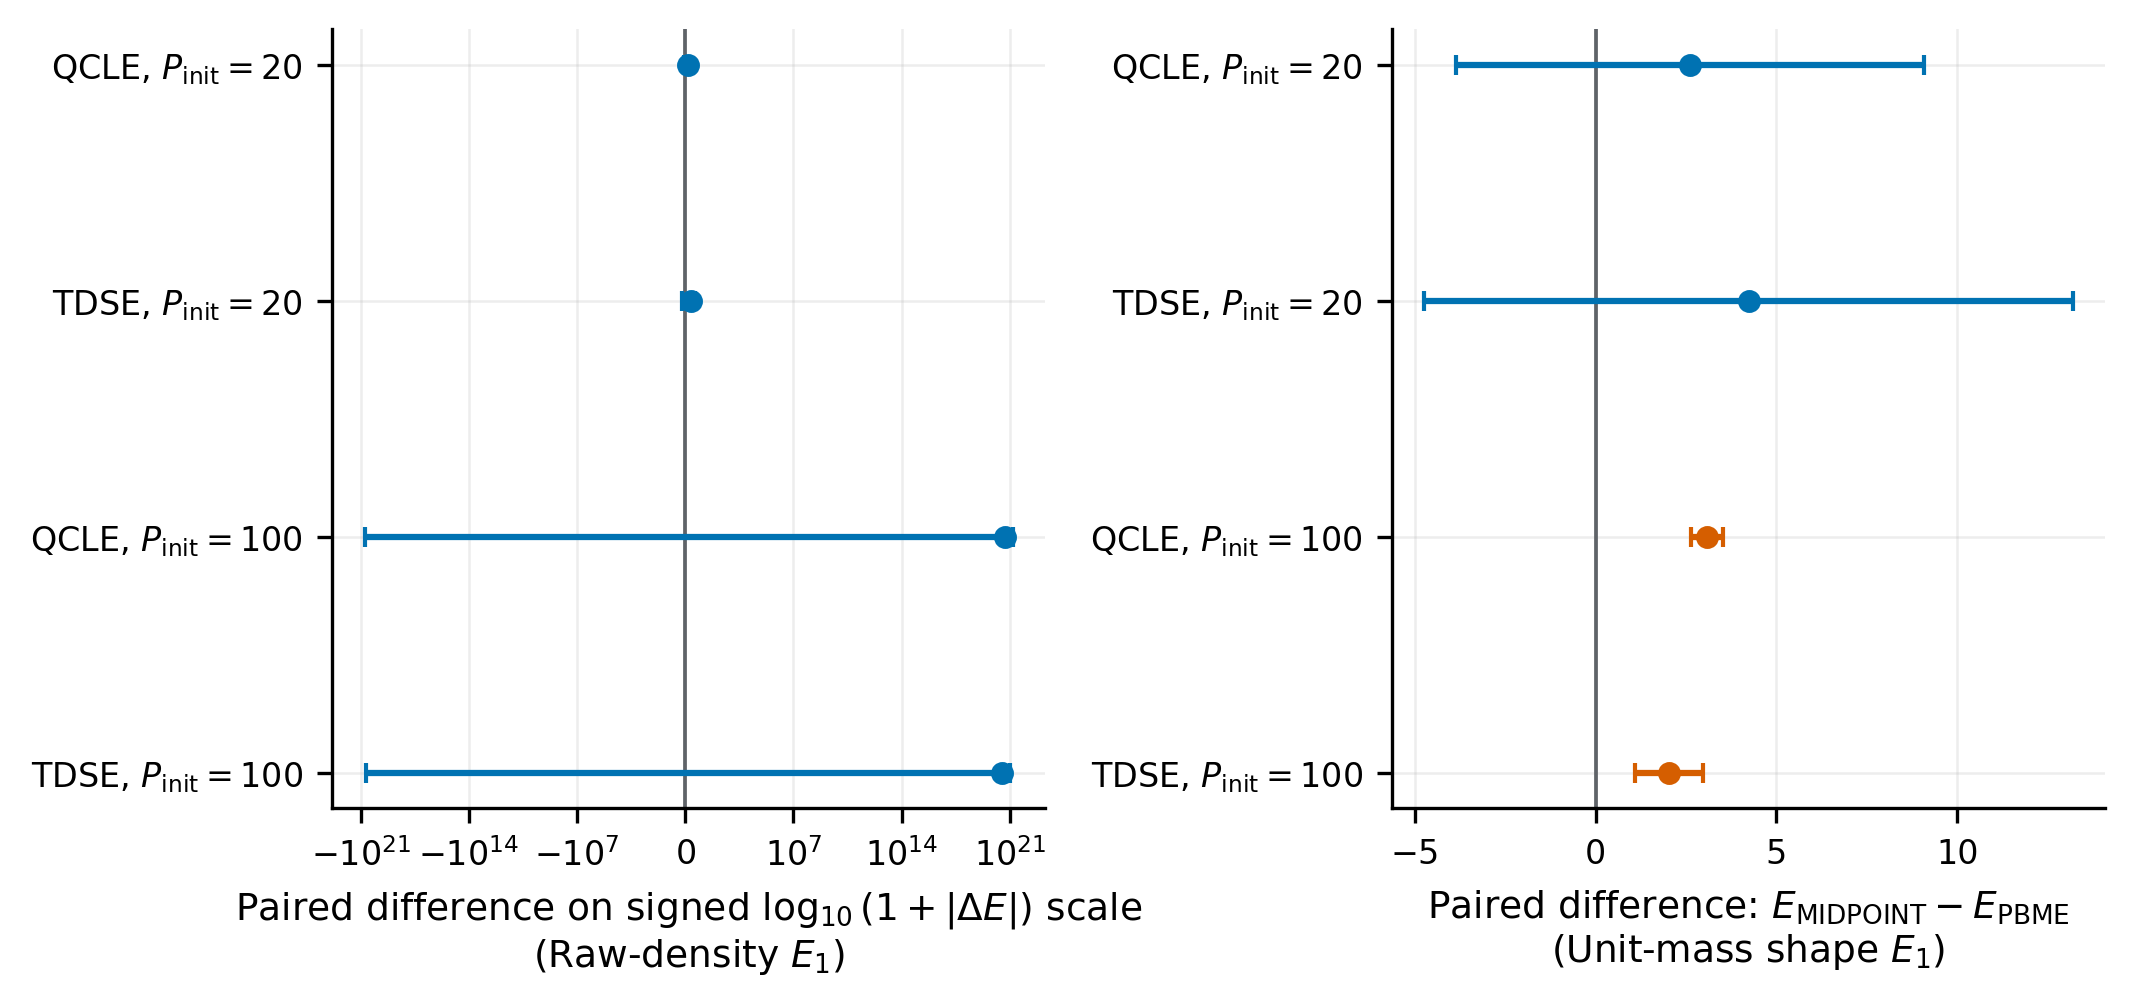
\includegraphics[width=0.96\textwidth]{../final_reviewer_closure/figures/paired_physical_reference_differences.png}
\caption{Four-seed paired MIDPOINT-minus-PBME differences for density
\(E_1\) errors against the matched TDSE and grid-QCLE references. Points are
paired means and bars are two-sided Student-\(t\) 95\% intervals with three
degrees of freedom. Positive values mean that MIDPOINT has the larger error.
The raw-density panel uses the signed display transform
\(\operatorname{sgn}(\Delta E)\log_{10}(1+\lvert\Delta E\rvert)\), whose tick
labels show the corresponding untransformed magnitude; the shape panel uses
unit-mass normalization and a linear axis. Shape agreement is therefore not
used as conservation evidence.}
\label{fig:paired-physical-reference-differences}
\end{figure}

\FloatBarrier

\section{Synthesis of the numerical evidence}
\label{sec:results-synthesis}

The positive identical-cloud reconstruction control establishes that the GP
can interpolate density values accurately under matched conditions. That
result does not carry through the sequence required by the physical
calculation. The manufactured derivative operator is non-monotone with cloud
size; the fitted density has substantial SEO-image leakage; the dynamical
response is dominated by cloud-to-cloud variation; and the raw MIDPOINT
normalization, trace, and energy can drift catastrophically. Controlled TDSE
and grid-QCLE references do not reveal a consistent physical-error reduction
relative to PBME. The failure is therefore not inferred from one diagnostic:
it is the common conclusion of independent operator, representation,
refinement, replication, conservation, and reference tests.

The defensible result is correspondingly narrow. The tested product-GP,
moving-cloud MIDPOINT discretization is not a reliable dynamical method for
this benchmark. This statement concerns the discretization studied here; it
does not constitute a failure of the continuum mapping-QCLE excess term.
% END INLINED CHAPTER 6

% BEGIN INLINED CHAPTER 7
\chapter{Discussion and Conclusions}
\label{chap:discussion-outlook}

This thesis set out to test whether a differentiable product-GP representation
could make the mapping-QCLE excess term usable on a moving trajectory cloud.
The answer for the construction studied here is no. Accurate interpolation of
density values on a fixed cloud does not imply accurate ambient derivatives,
preservation of the physical SEO image, stable signed estimators, or
conservative dynamics. The contribution is therefore a precisely defined
formulation, a sequence of physically interpretable tests that expose its
limitations, and concrete requirements for a successor. It is not a validated
GP-QCLE solver and it is not evidence that MIDPOINT improves PBME.

\section{Application-specific contribution}
\label{sec:discussion-contribution}

Values on a lower-dimensional manifold do not generally identify ambient
normal derivatives; that fact is not original to this thesis. The original
application-specific contribution is narrower: constructing a differentiable
product-GP excess-source prototype on moving PBME/MInt clouds, testing it
against an analytic manufactured operator and the exact two-state SEO image,
and connecting its observed derivative, projection, conservation, and
signed-weight failures to the propagated dynamics without claiming a unique
cause
\cite{Kim2008JCP,Kelly2012JCP,Raissi2017LinearGP,
Solak2002DerivativeGP,CockayneOatesSullivanGirolami2019}.

\section{Physical interpretation of the failure}
\label{sec:discussion-evidence}

The results in Chapter~\ref{chap:results} reveal a connected, but not uniquely
causal, failure pathway. A product kernel can reconstruct the sampled density
values while leaving ambient derivatives underdetermined away from the cloud.
The excess operator depends precisely on those derivatives. Once its source
is applied without enforcing the four-field SEO structure, the fitted density
can develop large components outside the physical image. The focused-sampling
ratio then combines sign cancellation with very large individual label ratios,
which magnifies cloud-to-cloud variation. The resulting raw normalization,
trace, and energy drift show that this is not merely a cosmetic change in
density shape.

These observations establish compatibility among the failure modes, not a
proof that one is the sole cause of the others. The manufactured operator
study, SEO projection diagnostic, signed-label analysis, and conservation
test deliberately isolate different links in the chain. Their agreement
supports the method-level conclusion without overstating causal identification.
The controlled TDSE and grid-QCLE studies then ensure that the absence of a
systematic physical improvement is not an artefact of an uncontrolled
reference calculation.

\section{Claim boundary}
\label{sec:discussion-limitations}

This thesis does not establish a validated discretization of the complete
mapping-basis QCLE, deterministic cloud convergence, strong uncertainty
calibration from four seeds, chemical accuracy outside the one-dimensional
two-state benchmark, multidimensional scalability, or systematic improvement
over PBME. TDSE and grid-QCLE have different epistemic roles: TDSE is
model-exact within numerical controls, whereas grid QCLE solves an approximate
quantum--classical equation numerically.

The production regularization \(0.05\), pilot \(0.01\), and
manufactured-test \(10^{-6}\) policies are all tested and reported rather than
conflated. The tail study demonstrates extreme signed-weight instability, but
its negligible-mass rule does not permit a nontrivial point-removal plateau,
so the instability is not assigned uniquely to small initial labels.

\section{Requirements for a successor}
\label{sec:discussion-successor}

A credible successor should regress the four real bath-dependent fields of the
two-state SEO image so that Hermiticity and projection are enforced by
construction. Its discrete excess source should preserve normalization and
the relevant trace and energy identities before any renormalization. The
regression should incorporate derivative information or structural constraints
capable of controlling directions normal to the sampled manifold. A future
success claim requires decreasing manufactured-operator errors under a
controlled refinement, time-step changes resolvable above seed variation,
independent-cloud uncertainty bands, raw conservation, and reproducibly
smaller PBME-matched errors against controlled references where the excess
source is appreciable
\cite{TraskBochevPerego2020,BonetLok1999,Monaghan2005}.

\section{Numerical scope and transferability}
\label{sec:discussion-numerical-scope}

The numerical conclusions are tied to the parameter ranges, independent seed
sets, domains, and discretizations stated in Chapter~\ref{chap:results} and
Appendix~\ref{app:reference-and-reproducibility}. Repeating those calculations
tests this particular construction on the same benchmark; it does not by
itself establish transferability to additional electronic states, nuclear
dimensions, coupling regimes, or sampling measures. Such transfer would
require renewed manufactured-operator, projection, conservation, and
reference comparisons rather than extrapolation from the present negative
result.

\section{Conclusion}
\label{sec:discussion-conclusions}

The combined numerical evidence supports a controlled negative result.
Accurate same-cloud value reconstruction does not guarantee an accurate
derivative-dependent excess operator, preservation of the SEO image, raw
conservation, or seed-stable dynamics. The tested MIDPOINT branch fails the
joint reliability criteria and does not demonstrate systematic improvement
over PBME. This conclusion applies to the tested discretization, not to the
continuum QCLE excess term.

Accordingly, the thesis contributes a precisely scoped formulation, a
physics-based failure analysis, and evidence-backed redesign criteria. It
does not claim that the tested construction is reliable, deterministically
cloud-converged, or improved.
% END INLINED CHAPTER 7

\appendix

\chapter[Initial Conditions and Sampling]{Initial Conditions, Sampling, and Cloud Quadrature}
\label{app:initial-conditions-sampling}
\addcontentsline{loa}{appendix}{%
  \protect\numberline{\thechapter}%
  Initial Conditions, Sampling, and Cloud Quadrature}

This appendix defines the numerical state carried by the moving support cloud
and documents the initial nuclear and mapping distributions used in the
production calculations. It also distinguishes full-dimensional importance
sampling from the singular focused mapping construction and states the
quadrature measure used for physical observables.

\section{State carried by the moving support cloud}
\label{appsec:cloud-state}

At time \(t_n\), the numerical state consists of the support cloud
\begin{equation}
\mathcal S_n
=
\left\{
\boldsymbol{\mathcal X}_i^n
\right\}_{i=1}^{N},
\label{appeq:support-cloud}
\end{equation}
the physical density labels
\begin{equation}
y_i^n
\approx
\tilde\rho_m
\left(
\boldsymbol{\mathcal X}_i^n,t_n
\right),
\label{appeq:live-physical-label}
\end{equation}
and a GP surrogate fitted to these data.

For the correction-weight implementation, the code stores the initial
sign-bearing labels \(y_i^0\) separately from the dimensionless array named
\texttt{correction\_}\allowbreak\texttt{weight}. No additional mathematical
label is introduced:
at step \(n\), the physical density label remains \(y_i^n\), and the stored
array represents the ratio \(y_i^n/y_i^0\) wherever that ratio is numerically
well defined. All derivations below are therefore written directly in terms
of \(y_i^n\), as in the main text.

For the product surrogate of Chapter~\ref{chap:gp-density-representation},
the transformed modulation labels are
\begin{equation}
u_i^n
=
\frac{
y_i^n
}{
g_{s,\mathrm{safe}}(\mathbf x_i^n)
},
\label{appeq:appendix-transformed-label}
\end{equation}
with \(g_{s,\mathrm{safe}}\) defined in
Eq.~\eqref{eq:seo-safe-profile}.  The vectors of physical and transformed
labels are
\[
\mathbf y^n
=
(y_1^n,\ldots,y_N^n)^T,
\qquad
\mathbf u^n
=
(u_1^n,\ldots,u_N^n)^T.
\]

\section{Initial nuclear and mapping distributions}
\label{appsec:initial-distributions}

\subsection{Gaussian nuclear Wigner density}
\label{appsubsec:nuclear-wigner}

For one bath degree of freedom, the initial nuclear wavepacket is
\begin{equation}
\psi(R)
\propto
\exp\left[
-\frac{(R-R_0)^2}{4\sigma_R^2}
+
\frac{i}{\hbar}P_{\rm init}(R-R_0)
\right].
\label{appeq:initial-gaussian-wavepacket}
\end{equation}
Its Wigner transform is
\begin{equation}
W_{\mathrm{cl}}(R,P)
=
\frac{1}{\pi\hbar}
\exp\left[
-\frac{(R-R_0)^2}{2\sigma_R^2}
-
\frac{2\sigma_R^2(P-P_{\rm init})^2}{\hbar^2}
\right].
\label{appeq:initial-nuclear-wigner}
\end{equation}
Consequently,
\begin{equation}
R\sim\mathcal N(R_0,\sigma_R^2),
\qquad
P\sim
\mathcal N
\left(
P_{\rm init},
\frac{\hbar^2}{4\sigma_R^2}
\right),
\label{appeq:nuclear-sampling-law}
\end{equation}
so that \(\sigma_P=\hbar/(2\sigma_R)\).

\subsection{Signed SEO sampling}
\label{appsubsec:signed-seo-sampling}

For an initially occupied subsystem state \(s\), the diagonal SEO kernel is
the analytic function
\begin{equation}
g_s(\mathbf x)
=
\mathcal G_{\mathrm{SEO}}(\mathbf x)
B_s(\mathbf x),
\label{appeq:seo-factorization}
\end{equation}
where
\begin{equation}
\mathcal G_{\mathrm{SEO}}(\mathbf x)
=
(\pi\hbar)^{-N_s}
\exp\left[
-\frac{\mathbf r^2+\mathbf p^2}{\hbar}
\right]
\label{appeq:seo-gaussian-envelope}
\end{equation}
and
\begin{equation}
B_s(\mathbf x)
=
\frac{2}{\hbar}
\left(
r_s^2+p_s^2
\right)
-1.
\label{appeq:seo-polynomial}
\end{equation}
The initial projected mapping density used by the sampler is
\begin{equation}
\tilde\rho_m(\boldsymbol{\mathcal X},0)
=
W_{\mathrm{cl}}(R,P)
g_s(\mathbf x).
\label{appeq:initial-projected-density}
\end{equation}

The standard signed-SEO proposal samples the bath variables from
\(W_{\mathrm{cl}}\) and the mapping variables from the positive Gaussian
envelope:
\begin{equation}
\pi_0(\boldsymbol{\mathcal X})
=
W_{\mathrm{cl}}(R,P)
\mathcal G_{\mathrm{SEO}}(\mathbf x).
\label{appeq:signed-seo-proposal}
\end{equation}
The associated importance ratio is
\begin{equation}
\frac{\tilde\rho_m(\boldsymbol{\mathcal X},0)}{\pi_0(\boldsymbol{\mathcal X})}
=
B_s(\mathbf x),
\label{appeq:signed-seo-weight}
\end{equation}
which carries the sign of the SEO Wigner density.

\subsection{Absolute-target sampling}
\label{appsubsec:absolute-target-sampling}

The optional absolute-target sampler uses
\begin{equation}
\pi_{\mathrm{abs}}(\boldsymbol{\mathcal X})
=
\frac{
|\tilde\rho_m(\boldsymbol{\mathcal X},0)|
}{
C_{\mathrm{abs}}
},
\qquad
C_{\mathrm{abs}}
=
\int
d\boldsymbol{\mathcal X}\,
|\tilde\rho_m(\boldsymbol{\mathcal X},0)|.
\label{appeq:absolute-target-proposal}
\end{equation}
The importance ratio is then
\begin{equation}
\frac{\tilde\rho_m(\boldsymbol{\mathcal X},0)}{\pi_{\mathrm{abs}}(\boldsymbol{\mathcal X})}
=
C_{\mathrm{abs}}
\operatorname{sgn}
\left[
\tilde\rho_m(\boldsymbol{\mathcal X},0)
\right].
\label{appeq:absolute-target-weight}
\end{equation}
Hence the magnitude of the importance factor is constant.  The implemented
rejection sampler uses a high quantile of \(|B_s|\) as a practical acceptance
ceiling; this is a variance-reduction device with an explicitly controlled
truncation bias.
This branch is inactive in the focused production and validation runs.
For the optional absolute-target branch, the campaign guide does not report
the selected quantile, realized ceiling, rejection rate, or induced truncation
bias. No numerical claim in this thesis relies on that inactive sampler.

\subsection{Focused MMST sampling}
\label{appsubsec:focused-sampling}

The focused occupation convention
\cite{StockThoss1997PRL,ThossStock1999PRA,Kelly2012JCP} is
\begin{equation}
n_\lambda
=
\frac{
r_\lambda^2+p_\lambda^2
}{
2\hbar
}
-\gamma.
\label{appeq:focused-occupation}
\end{equation}
For a trajectory focused on state \(s\),
\[
n_s=1,
\qquad
n_{\lambda\ne s}=0,
\]
and therefore
\begin{equation}
r_s^2+p_s^2
=
2\hbar(1+\gamma),
\qquad
r_{\lambda\ne s}^2+p_{\lambda\ne s}^2
=
2\hbar\gamma.
\label{appeq:focused-radii}
\end{equation}
The implementation uses \(\gamma=1/2\).  For the two-state problem,
\[
r_s^2+p_s^2=3\hbar,
\qquad
r_{\bar s}^2+p_{\bar s}^2=\hbar,
\]
where \(\bar s\) denotes the state different from \(s\).  Independent angles
\(\theta_\lambda\sim U(0,2\pi)\) determine
\begin{equation}
r_\lambda
=
\sqrt{2\hbar(n_\lambda+\gamma)}\cos\theta_\lambda,
\qquad
p_\lambda
=
\sqrt{2\hbar(n_\lambda+\gamma)}\sin\theta_\lambda.
\label{appeq:focused-angle-sampling}
\end{equation}

On the focused manifold, the mapping part of the SEO target has the constant
value
\begin{equation}
K_{\mathrm{focus}}
=
(\pi\hbar)^{-N_s}
\exp\left[
-2(1+N_s\gamma)
\right]
(4\gamma+3).
\label{appeq:focused-target-constant}
\end{equation}
The initial labels are therefore
\begin{equation}
y_i^0
=
W_{\mathrm{cl}}(R_i^0,P_i^0)
K_{\mathrm{focus}}.
\label{appeq:focused-initial-label}
\end{equation}
Focused sampling is supported on a product of circles in mapping space and is
therefore singular with respect to the full mapping-space Lebesgue measure.
This geometric fact is important when moment constraints and mapping-sector
length scales are interpreted.

\subsection{Frozen cloud quadrature measure}
\label{appsubsec:cloud-measure}

For a full-dimensional positive proposal density \(q_0\), the ordinary
importance measure is
defined at initialization by
\begin{equation}
\omega_i
=
\frac{
1
}{
Nq_0(\boldsymbol{\mathcal X}_i^0)
}.
\label{appeq:cloud-geometric-measure}
\end{equation}
It is then held fixed.  For a phase-space observable
\(A_m(\boldsymbol{\mathcal X})\),
\begin{equation}
\int
d\boldsymbol{\mathcal X}\,
A_m(\boldsymbol{\mathcal X})
\tilde\rho_m(\boldsymbol{\mathcal X},t_n)
\approx
\sum_{i=1}^{N}
\omega_i
A_m(\boldsymbol{\mathcal X}_i^n)
y_i^n.
\label{appeq:cloud-quadrature}
\end{equation}
The estimator is not self-normalized. An optional quantile cap on
\(\omega_i\) is implemented as a diagnostic variance-reduction measure and
must be reported whenever it is used.

Equation~\eqref{appeq:cloud-geometric-measure} does not apply to focused
mapping sampling, which is singular in the full mapping space. For the
focused production branch, the implemented frozen calibration may be written
as \(\omega_i^{\mathrm{focus}}=1/(Ny_i^0)\), so that
\begin{equation}
c_i^n
=
\omega_i^{\mathrm{focus}}y_i^n
=
\frac{1}{N}\frac{y_i^n}{y_i^0},
\qquad c_i^0=\frac{1}{N}.
\label{appeq:focused-cloud-coefficient}
\end{equation}
Here \(\omega_i^{\mathrm{focus}}\) is a conventional estimator calibration,
not the reciprocal of a full-dimensional proposal density.

\chapter[Hamiltonian Mapping Propagation]{Hamiltonian Mapping Propagation and the MInt Map}
\label{app:hamiltonian-mapping-propagation}
\addcontentsline{loa}{appendix}{%
  \protect\numberline{\thechapter}%
  Hamiltonian Mapping Propagation and the MInt Map}

This appendix gives the trace--traceless mapping Hamiltonian and the symmetric
MInt factorization used to propagate the PBME characteristics. These formulas
concern Hamiltonian support motion only; the excess density source is developed
separately in Appendix~\ref{app:excess-liouvillian}.

\section{PBME Hamiltonian and the MInt map}
\label{appsec:mint-derivation}

\subsection{Trace--traceless mapping Hamiltonian}
\label{appsubsec:mint-hamiltonian}

The mapping Hamiltonian is
\begin{equation}
H_m(\boldsymbol{\mathcal X})
=
\frac{\mathbf P^2}{2M}
+
V_0(\mathbf R)
+
\frac{1}{2\hbar}
\left[
\mathbf r^T\bar h(\mathbf R)\mathbf r
+
\mathbf p^T\bar h(\mathbf R)\mathbf p
\right].
\label{appeq:appendix-mapping-hamiltonian}
\end{equation}
For the one-dimensional numerical model,
\begin{align}
\dot R
&=
\frac{P}{M},
\\
\dot P
&=
-\frac{dV_0}{dR}
-
\frac{1}{2\hbar}
\left[
\mathbf r^T
\frac{d\bar h}{dR}
\mathbf r
+
\mathbf p^T
\frac{d\bar h}{dR}
\mathbf p
\right],
\\
\dot{\mathbf r}
&=
\frac{1}{\hbar}\bar h(R)\mathbf p,
\\
\dot{\mathbf p}
&=
-\frac{1}{\hbar}\bar h(R)\mathbf r.
\end{align}

For the dual avoided-crossing model,
\begin{equation}
h(R)
=
\begin{pmatrix}
V^{11}(R) & V^{12}(R)\\
V^{12}(R) & V^{22}(R)
\end{pmatrix},
\label{appeq:tully-diabatic-hamiltonian}
\end{equation}
with
\begin{align}
V^{11}(R)&=0,
\\
V^{22}(R)&=-A e^{-BR^2}+E_0,
\\
V^{12}(R)&=C e^{-DR^2},
\end{align}
and
\begin{align}
\frac{dV^{11}}{dR}&=0,
\\
\frac{dV^{22}}{dR}
&=
2ABR\,e^{-BR^2},
\\
\frac{dV^{12}}{dR}
&=
-2CDR\,e^{-DR^2}.
\end{align}
The trace--traceless decomposition is
\begin{equation}
V_0(R)
=
\frac{1}{2}
\operatorname{Tr}_{\mathrm s}h(R),
\qquad
\bar h(R)
=
h(R)-V_0(R)I_{\mathrm s}.
\label{appeq:tully-trace-traceless}
\end{equation}

\subsection{Symmetric splitting}
\label{appsubsec:mint-splitting}

Write
\[
H_m=H_A+H_B,
\qquad
H_A=\frac{P^2}{2M},
\qquad
H_B
=
V_0(R)
+
\frac{1}{2\hbar}
\left[
\mathbf r^T\bar h(R)\mathbf r
+
\mathbf p^T\bar h(R)\mathbf p
\right].
\]
The MInt step is
\begin{equation}
\Psi_\tau^{\mathrm{MInt}}
=
\mathcal A_{\tau/2}
\circ
\mathcal B_\tau
\circ
\mathcal A_{\tau/2}.
\label{appeq:mint-composition}
\end{equation}
The first drift gives
\begin{equation}
R_{1/2}
=
R_0+\frac{\tau}{2M}P_0.
\label{appeq:mint-first-drift}
\end{equation}

At fixed \(R_{1/2}\), diagonalize
\begin{equation}
\bar h(R_{1/2})
=
\mathsf U_{\mathrm{loc}}
\boldsymbol\varepsilon
\mathsf U_{\mathrm{loc}}^T,
\label{appeq:mint-local-diagonalization}
\end{equation}
where \(\boldsymbol\varepsilon=\operatorname{diag}
(\varepsilon_1,\ldots,\varepsilon_{N_s})\).  Define
\[
\widetilde{\mathbf r}
=
\mathsf U_{\mathrm{loc}}^T\mathbf r,
\qquad
\widetilde{\mathbf p}
=
\mathsf U_{\mathrm{loc}}^T\mathbf p.
\]
The fixed-\(R\) mapping equations are decoupled rotations:
\begin{align}
\widetilde{\mathbf r}(\tau)
&=
\cos\left(
\frac{\tau\boldsymbol\varepsilon}{\hbar}
\right)
\widetilde{\mathbf r}(0)
+
\sin\left(
\frac{\tau\boldsymbol\varepsilon}{\hbar}
\right)
\widetilde{\mathbf p}(0),
\\
\widetilde{\mathbf p}(\tau)
&=
\cos\left(
\frac{\tau\boldsymbol\varepsilon}{\hbar}
\right)
\widetilde{\mathbf p}(0)
-
\sin\left(
\frac{\tau\boldsymbol\varepsilon}{\hbar}
\right)
\widetilde{\mathbf r}(0).
\label{appeq:mint-mapping-rotation}
\end{align}

\subsection{Analytic bath-momentum integral}
\label{appsubsec:mint-momentum-integral}

Let
\begin{equation}
\mathsf G
=
\mathsf U_{\mathrm{loc}}^T
\frac{d\bar h}{dR}
\mathsf U_{\mathrm{loc}},
\qquad
\omega_{ab}
=
\frac{
\varepsilon_a-\varepsilon_b
}{
\hbar
}.
\label{appeq:mint-local-force-matrix}
\end{equation}
Introduce
\begin{align}
\mathsf C_{ab}
&=
\widetilde r_a\widetilde r_b
+
\widetilde p_a\widetilde p_b,
\\
\mathsf S_{ab}
&=
\widetilde p_a\widetilde r_b
-
\widetilde r_a\widetilde p_b.
\end{align}
The oscillatory integrals are
\begin{align}
I_c(\omega,\tau)
&=
\int_0^\tau
\cos(\omega t)\,dt
=
\tau
\cos\left(\frac{\omega\tau}{2}\right)
\operatorname{sinc}
\left(\frac{\omega\tau}{2}\right),
\\
I_s(\omega,\tau)
&=
\int_0^\tau
\sin(\omega t)\,dt
=
\tau
\sin\left(\frac{\omega\tau}{2}\right)
\operatorname{sinc}
\left(\frac{\omega\tau}{2}\right),
\label{appeq:mint-stable-integrals}
\end{align}
where \(\operatorname{sinc}(x)=\sin(x)/x\).  These expressions remain regular
as \(\omega\rightarrow0\).

The exact fixed-\(R\) mapping-force integral is
\begin{equation}
I_{\mathrm{map}}(\tau)
=
\sum_{a,b}
\mathsf G_{ab}
\left[
\mathsf C_{ab}I_c(\omega_{ab},\tau)
+
\mathsf S_{ab}I_s(\omega_{ab},\tau)
\right].
\label{appeq:mint-exact-force-integral}
\end{equation}
Hence
\begin{equation}
P_1
=
P_0
-
\tau
\frac{dV_0}{dR}(R_{1/2})
-
\frac{1}{2\hbar}
I_{\mathrm{map}}(\tau),
\label{appeq:mint-momentum-update}
\end{equation}
and the closing drift is
\begin{equation}
R_1
=
R_{1/2}
+
\frac{\tau}{2M}P_1.
\label{appeq:mint-closing-drift}
\end{equation}

The mapping rotation preserves
\begin{equation}
\mathcal R_m^2
=
\mathbf r^T\mathbf r+\mathbf p^T\mathbf p,
\label{appeq:mint-radius-invariant}
\end{equation}
and MInt is symmetric and symplectic.  The numerical checks use the
round-trip residual
\begin{equation}
\varepsilon_{\mathrm{rt}}
=
\frac{
\left\|
\Psi_{-\tau}^{\mathrm{MInt}}
\left[
\Psi_\tau^{\mathrm{MInt}}
(\boldsymbol{\mathcal X})
\right]
-
\boldsymbol{\mathcal X}
\right\|
}{
1+\|\boldsymbol{\mathcal X}\|
}
\label{appeq:mint-roundtrip}
\end{equation}
and the symplectic residual
\begin{equation}
\varepsilon_{\mathrm{symp}}
=
\frac{
\left\|
\left(D\Psi_\tau^{\mathrm{MInt}}\right)^T
\mathbb J
D\Psi_\tau^{\mathrm{MInt}}
-
\mathbb J
\right\|_F
}{
\|\mathbb J\|_F
}.
\label{appeq:mint-symplectic-residual}
\end{equation}

\chapter[GP Density and Derivatives]{Gaussian-Process Density Representation and Analytic Derivatives}
\label{app:gp-density-derivatives}
\addcontentsline{loa}{appendix}{%
  \protect\numberline{\thechapter}%
  Gaussian-Process Density Representation and Analytic Derivatives}

This appendix collects the finite Gaussian-process representations, analytic
kernel and SEO-profile derivatives, hyperparameter objectives, and moment
constraints. The product representation is the production architecture used
for the reported calculations. Direct-density and density-difference forms are
retained as explicitly identified alternatives and should not be inferred to
have generated the MIDPOINT results unless stated otherwise.

\section{Gaussian-process density representations}
\label{appsec:gp-representations}

\subsection{Product representation used in the thesis}
\label{appsubsec:product-representation}

The structured density representation is
\begin{equation}
\widehat{\rho}_{m,t}
(\boldsymbol{\mathcal X})
=
g_s(\mathbf x)
\mu_t(\boldsymbol{\mathcal X}),
\label{appeq:appendix-product-density}
\end{equation}
where
\begin{equation}
\mu_t(\boldsymbol{\mathcal X})
=
\sum_{j=1}^{N}
\zeta_j(t)
k_{\boldsymbol\theta_t}
\left(
\boldsymbol{\mathcal X},
\boldsymbol{\mathcal X}_j(t)
\right).
\label{appeq:appendix-modulation-expansion}
\end{equation}
The coefficients satisfy
\begin{equation}
\boldsymbol\zeta_t
=
K_{y,t}^{-1}\mathbf u_t,
\qquad
K_{y,t}=K_t+\sigma_n^2I.
\label{appeq:appendix-coefficient-solve}
\end{equation}
The exact \(g_s\) is used in prediction and differentiation.  The safe profile
appears only in the label transformation
Eq.~\eqref{appeq:appendix-transformed-label}.

\subsection{Optional direct-density GP}
\label{appsubsec:direct-density-gp}

The formulation also admits a direct-density branch,
\begin{equation}
\widehat{\rho}_{m,t}^{\mathrm{dir}}
(\boldsymbol{\mathcal X})
=
\sum_{j=1}^{N}
\zeta_j^{\mathrm{dir}}(t)
k_{\boldsymbol\theta_t}
\left(
\boldsymbol{\mathcal X},
\boldsymbol{\mathcal X}_j(t)
\right),
\label{appeq:direct-density-gp}
\end{equation}
with
\[
\boldsymbol\zeta_t^{\mathrm{dir}}
=
K_{y,t}^{-1}\mathbf y_t.
\]
This branch approximates the full density directly and must not be confused
with the product representation of
Eq.~\eqref{appeq:appendix-product-density}.  In particular, its kernel
derivatives supply the complete density derivatives, whereas the product
branch requires the derivatives of both \(g_s\) and \(\mu_t\).

\subsection{Density-difference representation}
\label{appsubsec:density-difference}

The density-difference branch decomposes the density as
\begin{align}
\widehat{\rho}_{m,t}^{\mathrm{diff}}
(\boldsymbol{\mathcal X})
&=
\widehat{\rho}_{m,0}
\left[
\mathcal F_{-t}^{\circ}
(\boldsymbol{\mathcal X})
\right]
\nonumber\\
&\quad+
\sum_{j=1}^{N}
\zeta_j^{\Delta}(t)
 k_{\boldsymbol\theta_t}
\left(
\boldsymbol{\mathcal X},
\boldsymbol{\mathcal X}_j(t)
\right).
\label{appeq:density-difference-representation}
\end{align}
The superscript \(\Delta\) is a branch qualifier on the GP coefficients; it
does not denote an additional physical density. The PBME Hamiltonian flow
\(\mathcal F_t^\circ\) is already defined in
Chapter~\ref{chap:density-level-integration}. At the transported support
points,
\[
\mathcal F_{-t}^{\circ}
\left(
\boldsymbol{\mathcal X}_i(t)
\right)
=
\boldsymbol{\mathcal X}_i(0).
\]
The baseline GP is frozen after its initial fit, and the correction
coefficients \(\boldsymbol\zeta_t^{\Delta}\) are obtained from the residual
physical labels
\begin{equation}
y_i(t)-y_i(0).
\label{appeq:density-difference-label}
\end{equation}

In the present implementation, the off-support transported baseline is
approximated by moving the baseline kernel centres with the support cloud.
This identity is exact at the support points but is not an exact pullback of
each kernel under a nonlinear MInt map.  The density-difference architecture
is therefore a distinct approximation and is reported separately from the
product representation.  The current software does not combine the
density-difference and product branches.

\section{ARD squared-exponential kernel derivatives}
\label{appsec:ard-derivatives}

For a kernel section centred at
\(\boldsymbol{\mathcal X}_j(t)\), write
\begin{equation}
k_j(\boldsymbol{\mathcal X})
=
\sigma_f^2
\exp\left[
-\frac{1}{2}
\sum_d
\frac{
(\mathcal X_d-\mathcal X_{j,d})^2
}{
\ell_d^2
}
\right],
\label{appeq:ard-kernel}
\end{equation}
and define
\begin{equation}
q_{j,d}
=
\frac{
\mathcal X_{j,d}-\mathcal X_d
}{
\ell_d^2
}.
\label{appeq:ard-q-definition}
\end{equation}
Then
\begin{equation}
\partial_d k_j
=
q_{j,d}k_j.
\label{appeq:ard-first}
\end{equation}
Differentiating once more gives
\begin{equation}
\partial_e\partial_d k_j
=
\left(
q_{j,e}q_{j,d}
-
\frac{\delta_{de}}{\ell_d^2}
\right)
k_j.
\label{appeq:ard-second}
\end{equation}
A third derivative is
\begin{align}
\partial_f\partial_e\partial_d k_j
&=
\Bigg[
q_{j,f}q_{j,e}q_{j,d}
-
\frac{\delta_{de}}{\ell_d^2}q_{j,f}
-
\frac{\delta_{df}}{\ell_d^2}q_{j,e}
-
\frac{\delta_{ef}}{\ell_e^2}q_{j,d}
\Bigg]
k_j.
\label{appeq:ard-third}
\end{align}
For one bath momentum component \(P\) and mapping coordinates
\(x_d,x_e\), the bath and mapping components are independent, so
\begin{equation}
\frac{\partial^3k_j}
{\partial x_e\partial x_d\partial P}
=
q_{j,P}
\left(
q_{j,e}q_{j,d}
-
\frac{\delta_{de}}{\ell_d^2}
\right)
k_j.
\label{appeq:ard-qcle-third}
\end{equation}
The derivatives of \(\mu_t\) are obtained by summing
Eqs.~\eqref{appeq:ard-first}--\eqref{appeq:ard-qcle-third} with coefficients
\(\zeta_j(t)\).

\section{Derivatives of the SEO profile and the product density}
\label{appsec:product-derivatives}

Write
\[
g_s(\mathbf x)
=
\mathcal G_{\mathrm{SEO}}(\mathbf x)
B_s(\mathbf x),
\]
with \(\mathcal G_{\mathrm{SEO}}\) and \(B_s\) defined in
Eqs.~\eqref{appeq:seo-gaussian-envelope} and
\eqref{appeq:seo-polynomial}.  For a mapping coordinate \(x_d\), where
\(x_d\) denotes either an \(r_\lambda\) or a \(p_\lambda\) component,
\begin{equation}
\partial_d
\mathcal G_{\mathrm{SEO}}
=
-\frac{2x_d}{\hbar}
\mathcal G_{\mathrm{SEO}}.
\label{appeq:seo-envelope-first}
\end{equation}
The polynomial derivatives are
\begin{equation}
\frac{\partial B_s}{\partial r_\lambda}
=
\frac{4}{\hbar}
\delta_{\lambda s}r_s,
\qquad
\frac{\partial B_s}{\partial p_\lambda}
=
\frac{4}{\hbar}
\delta_{\lambda s}p_s,
\label{appeq:seo-polynomial-first}
\end{equation}
and
\begin{equation}
\frac{\partial^2B_s}
{\partial r_{\lambda'}\partial r_\lambda}
=
\frac{4}{\hbar}
\delta_{\lambda s}\delta_{\lambda's},
\qquad
\frac{\partial^2B_s}
{\partial p_{\lambda'}\partial p_\lambda}
=
\frac{4}{\hbar}
\delta_{\lambda s}\delta_{\lambda's}.
\label{appeq:seo-polynomial-second}
\end{equation}

The first derivative of the profile is
\begin{equation}
\partial_d g_s
=
\mathcal G_{\mathrm{SEO}}
\left[
\partial_dB_s
-
\frac{2x_d}{\hbar}B_s
\right],
\label{appeq:seo-profile-first}
\end{equation}
and the second derivative is
\begin{align}
\partial_e\partial_d g_s
&=
\mathcal G_{\mathrm{SEO}}
\Bigg[
\partial_e\partial_dB_s
-
\frac{2x_e}{\hbar}\partial_dB_s
-
\frac{2x_d}{\hbar}\partial_eB_s
\nonumber\\
&\hspace{6em}
+
\left(
\frac{4x_dx_e}{\hbar^2}
-
\frac{2\delta_{ab}}{\hbar}
\right)
B_s
\Bigg].
\label{appeq:seo-profile-second}
\end{align}

For the static product profile, \(g_s\) is independent of \(\mathbf R\) and
\(\mathbf P\).  The mixed third derivative required by the excess operator is
therefore
\begin{align}
\frac{\partial^3\widehat{\rho}_{m,t}}
{\partial x_e\partial x_d\partial P}
&=
\frac{\partial^2g_s}
{\partial x_e\partial x_d}
\frac{\partial\mu_t}{\partial P}
+
\frac{\partial g_s}{\partial x_d}
\frac{\partial^2\mu_t}
{\partial x_e\partial P}
\nonumber\\
&\quad
+
\frac{\partial g_s}{\partial x_e}
\frac{\partial^2\mu_t}
{\partial x_d\partial P}
+
g_s
\frac{\partial^3\mu_t}
{\partial x_e\partial x_d\partial P}.
\label{appeq:static-product-third}
\end{align}
This is the exact product rule used for the static product surrogate.

\subsection{Transported SEO profile}
\label{appsubsec:transported-profile}

The transported-profile branch stores a mapping footpoint
\(\mathbf x_i^0\) for each support trajectory and represents
\begin{equation}
g_{s,t}^{\mathrm{tr}}
(\boldsymbol{\mathcal X}_i^t)
=
g_s(\mathbf x_i^0).
\label{appeq:transported-profile}
\end{equation}
Let
\(
D\mathbf x_i^0
=
D_{\boldsymbol{\mathcal X}_i^t}\mathbf x_i^0
\)
denote the Jacobian of the mapping footpoint with respect to the current
extended phase-space point. The implemented gradient is
\begin{equation}
\nabla_{\boldsymbol{\mathcal X}^t}
 g_{s,t}^{\mathrm{tr}}
=
\left(D\mathbf x^0\right)^T
\nabla_{\mathbf x^0}g_s.
\label{appeq:transported-profile-first}
\end{equation}
The implemented Hessian retains only the product of first footpoint
derivatives,
\begin{equation}
\nabla_{\boldsymbol{\mathcal X}^t}^{2}
 g_{s,t}^{\mathrm{tr}}
\approx
\left(D\mathbf x^0\right)^T
\nabla_{\mathbf x^0}^{2}g_s
\left(D\mathbf x^0\right).
\label{appeq:transported-profile-derivatives}
\end{equation}
The omitted term is the contraction of
\(\nabla_{\mathbf x^0}g_s\) with the Hessian
\(D^2\mathbf x^0\) of the footpoint map. Accordingly,
Eq.~\eqref{appeq:transported-profile-derivatives} is an approximation rather
than the exact Hessian of the pulled-back profile.

For a profile that depends on \(P\) through the transported footpoint, the
implemented Leibniz expansion is
\begin{align}
\partial_d\partial_e\partial_P(g\mu)
&\approx
g_{de}\mu_P
+
g_{dP}\mu_e
+
g_d\mu_{eP}
+
g_{eP}\mu_d
\nonumber\\
&\quad
+
g_e\mu_{dP}
+
g_P\mu_{de}
+
g\mu_{deP}.
\label{appeq:transported-product-third}
\end{align}
The pure profile term \(g_{deP}\mu\) is omitted because the current transported
profile stores only first-order footpoint geometry.  This seven-term closure
must therefore be distinguished from the exact static-profile formula
Eq.~\eqref{appeq:static-product-third}.

\section{GP hyperparameters and physical moment constraints}
\label{appsec:gp-fitting}

\subsection{Kernel system and optimization objectives}
\label{appsubsec:gp-objectives}

The regularized kernel matrix is
\begin{equation}
K_y
=
K+\sigma_n^2I+\epsilon_{\mathrm{jit}}I.
\label{appeq:appendix-Ky}
\end{equation}
The negative log marginal likelihood for a label vector \(\mathbf d\) is
\begin{equation}
\mathcal J_{\mathrm{NMLL}}
=
\frac{1}{2}
\mathbf d^T K_y^{-1}\mathbf d
+
\frac{1}{2}\log\det K_y
+
\frac{N}{2}\log(2\pi),
\label{appeq:appendix-nmll}
\end{equation}
where \(\mathbf d=\mathbf u\) for the product GP and
\(\mathbf d=\mathbf y\) for the direct-density GP.

For the LOO objective, define the precision matrix
\begin{equation}
\mathsf P
=
K_y^{-1},
\qquad
\boldsymbol\zeta
=
\mathsf P\mathbf d.
\label{appeq:appendix-precision}
\end{equation}
The exact LOO residual is
\begin{equation}
e_i^{\mathrm{LOO}}
=
\frac{
\zeta_i
}{
\mathsf P_{ii}
},
\label{appeq:appendix-loo}
\end{equation}
and the corresponding mean-square objective is
\[
\mathcal J_{\mathrm{LOO}}
=
\frac{1}{N}
\sum_{i=1}^{N}
\left(
e_i^{\mathrm{LOO}}
\right)^2.
\]

The numerical implementation permits frozen, breathing, adaptive, and free refit
policies described in Sec.~\ref{sec:gp-hyperparameter-policies}.  The
hyperparameters used to construct a source operator are held fixed during
that operator evaluation or source leg.

\subsection{Karush--Kuhn--Tucker/Schur-complement projection}
\label{appsubsec:kkt-projection}

The Karush--Kuhn--Tucker (KKT) formulation is used for the linear moment
constraints. Let \(\psi_c(\boldsymbol{\mathcal X})\) denote a constrained physical moment,
and define
\begin{equation}
\left(\mathsf C_{\mathrm{mom}}\right)_{cj}
=
\int
d\boldsymbol{\mathcal X}\,
\psi_c(\boldsymbol{\mathcal X})
k_j(\boldsymbol{\mathcal X}).
\label{appeq:kkt-moment-matrix}
\end{equation}
For the direct-density branch, the constrained coefficient vector minimizes
\begin{equation}
\frac{1}{2}
\left(
\boldsymbol\zeta-\boldsymbol\zeta_0
\right)^T
K_y
\left(
\boldsymbol\zeta-\boldsymbol\zeta_0
\right)
\label{appeq:kkt-objective}
\end{equation}
subject to
\begin{equation}
\mathsf C_{\mathrm{mom}}\boldsymbol\zeta
=
\mathbf m,
\label{appeq:kkt-constraints}
\end{equation}
where
\(\boldsymbol\zeta_0=K_y^{-1}\mathbf y\).  The Lagrangian stationarity
conditions give
\[
K_y
\left(
\boldsymbol\zeta-\boldsymbol\zeta_0
\right)
+
\mathsf C_{\mathrm{mom}}^T\boldsymbol\xi_{\mathrm K}
=
0,
\]
and therefore
\[
\boldsymbol\zeta
=
\boldsymbol\zeta_0
-
K_y^{-1}\mathsf C_{\mathrm{mom}}^T
\boldsymbol\xi_{\mathrm K}.
\]
Substitution into Eq.~\eqref{appeq:kkt-constraints} yields
\[
\left(
\mathsf C_{\mathrm{mom}} K_y^{-1}\mathsf C_{\mathrm{mom}}^T
\right)
\boldsymbol\xi_{\mathrm K}
=
\mathsf C_{\mathrm{mom}}\boldsymbol\zeta_0-\mathbf m.
\]
Hence
\begin{equation}
\boldsymbol\zeta
=
\boldsymbol\zeta_0
-
K_y^{-1}\mathsf C_{\mathrm{mom}}^T
\left(
\mathsf C_{\mathrm{mom}} K_y^{-1}\mathsf C_{\mathrm{mom}}^T
\right)^{+}
\left(
\mathsf C_{\mathrm{mom}}\boldsymbol\zeta_0-\mathbf m
\right)
\label{appeq:kkt-solution}
\end{equation}
where \(+\) denotes the rank-revealing pseudoinverse.  The implementation adds
a small ridge to the Schur matrix and uses a singular-value decomposition
(SVD) to remove numerically null constraint directions.

The constraint contract depends on the density representation and sampling
geometry.  Signed-SEO direct-density fits may enforce normalization, subsystem
trace, and energy.  Focused labels do not define a regular six-dimensional
density fit and therefore disable this projection.  The current product
wrapper also disables the direct-GP KKT rows because those rows integrate the
inner modulation \(\mu_t\), whereas the physical moments involve the product
\(g_s\mu_t\).  Applying the direct-GP moment matrix to the inner GP would impose
the wrong physical constraints.


\section{Support locality and derivative identifiability}
\label{appsec:support-locality-identifiability}

For a zero-mean ARD squared-exponential posterior mean with a finite set of
centres, define the kernel-scaled distance to the support by
\begin{equation}
d_{\boldsymbol\theta}
\left(
\boldsymbol{\mathcal X},\mathcal S_t
\right)
=
\min_j
\left[
\sum_{a=1}^{D}
\frac{
\left(
\mathcal X_a-\mathcal X_{j,a}(t)
\right)^2
}{\ell_a^2}
\right]^{1/2}.
\label{appeq:scaled-support-distance}
\end{equation}
The finite expansion satisfies
\begin{equation}
\left|
\mu_t^{(N)}(\boldsymbol{\mathcal X})
\right|
\le
\sigma_f^2
\left\|\boldsymbol\zeta_t\right\|_1
\exp\left[
-\frac{1}{2}
d_{\boldsymbol\theta}
\left(
\boldsymbol{\mathcal X},\mathcal S_t
\right)^2
\right].
\label{appeq:gp-locality-bound}
\end{equation}
This bound describes the locality of the chosen finite representation. It does
not imply that the continuum density vanishes away from the support. It states
that the posterior mean has no data-driven control there and reverts toward
its prior according to the kernel geometry.

On a target region $\Omega$, the Euclidean fill distance is
\begin{equation}
h_{\Omega,\mathcal S_t}
=
\sup_{\boldsymbol{\mathcal X}\in\Omega}
\min_i
\left\|
\boldsymbol{\mathcal X}-\boldsymbol{\mathcal X}_i(t)
\right\|.
\label{appeq:fill-distance}
\end{equation}
Approximation bounds on a compact region depend on this quantity, the kernel
smoothness, and the regularity of the target
\cite{Wendland2005,SchabackWendland2006}. A finite empirical cloud and a
smooth finite-bandwidth kernel expansion are mathematically different
numerical objects; agreement of cloud quadrature and analytic GP integration
must therefore be tested rather than assumed
\cite{HosseiniNigamStockie2016}.

Focused MMST sampling further places the mapping variables on a constrained
shell whose total radius is preserved by the Hamiltonian map. Values of a
multivariate function on this lower-dimensional manifold do not, in general,
determine derivatives normal to it. The kernel prior selects one smooth
continuation of the modulation $\mu_t$, but that continuation is a modeling
assumption rather than information independently supplied by the focused data.
This is especially important for the mixed mapping derivatives entering the
excess operator. The analytic SEO factor reduces the ambiguity by supplying
known mapping-space structure, but it does not eliminate the need for
off-manifold validation of the evolving modulation.

\chapter[Excess Liouvillian]{Excess Mapping Liouvillian and Semi-Discrete Source Operator}
\label{app:excess-liouvillian}
\addcontentsline{loa}{appendix}{%
  \protect\numberline{\thechapter}%
  Excess Mapping Liouvillian and Semi-Discrete Source Operator}

This appendix derives the differential action of the excess mapping
Liouvillian for the supported density representations. It includes the
conservative flux form, the backward-map derivative tensors needed by the
pulled-back path, and the matrices used to collocate the source on the moving
support.

\section{Excess mapping-QCLE operator}
\label{appsec:excess-operator}

\subsection{General operator and one-dimensional specialization}
\label{appsubsec:excess-operator-form}

The thesis defines
\[
\mathcal Q=-i\mathcal L_m'.
\]
For a general bath,
\begin{align}
\mathcal Q[f]
&=
-\frac{\hbar}{8}
\sum_{\lambda,\lambda'=1}^{N_s}
\nabla_{\mathbf R}
\bar h^{\lambda\lambda'}(\mathbf R)
\cdot
\left[
\left(
\frac{\partial^2}
{\partial r_{\lambda'}\partial r_\lambda}
+
\frac{\partial^2}
{\partial p_{\lambda'}\partial p_\lambda}
\right)
\nabla_{\mathbf P}f
\right].
\label{appeq:general-excess-operator}
\end{align}
For the one-dimensional Tully implementation,
\begin{align}
\mathcal Q[f]
&=
-\frac{\hbar}{8}
\sum_{\lambda,\lambda'=1}^{2}
\frac{d\bar h^{\lambda\lambda'}(R)}{dR}
\left[
\frac{\partial^3 f}
{\partial P\partial r_{\lambda'}\partial r_\lambda}
+
\frac{\partial^3 f}
{\partial P\partial p_{\lambda'}\partial p_\lambda}
\right].
\label{appeq:one-dimensional-excess-operator}
\end{align}

The sign in Eq.~\eqref{appeq:one-dimensional-excess-operator} is included in
\(\mathcal Q\).  The characteristic equation is therefore
\begin{equation}
\frac{d}{dt}
\tilde\rho_m
\left(
\boldsymbol{\mathcal X}(t),t
\right)
=
\mathcal Q[\tilde\rho_m]
\left(
\boldsymbol{\mathcal X}(t),t
\right),
\label{appeq:appendix-characteristic-density}
\end{equation}
and a midpoint label update contains \(+\Delta t\,\mathcal Q\), not a second
minus sign.

\subsection{Direct-density GP contraction}
\label{appsubsec:direct-q-contraction}

For the direct-density GP of
Eq.~\eqref{appeq:direct-density-gp}, substitution of
Eq.~\eqref{appeq:ard-qcle-third} into
Eq.~\eqref{appeq:one-dimensional-excess-operator} gives
\begin{align}
\mathcal Q
\left[
\widehat{\rho}_{m,t}^{\mathrm{dir}}
\right]
(\boldsymbol{\mathcal X})
&=
-\frac{\hbar}{8}
\sum_{j=1}^{N}
\zeta_j^{\mathrm{dir}}(t)
q_{j,P}k_j
\nonumber\\
&\quad\times
\sum_{\lambda,\lambda'=1}^{2}
\frac{d\bar h^{\lambda\lambda'}}{dR}
\Bigg[
q_{j,r_{\lambda'}}
q_{j,r_\lambda}
-
\frac{
\delta_{\lambda\lambda'}
}{
\ell_{r_\lambda}^2
}
\nonumber\\
&\hspace{11em}
+
q_{j,p_{\lambda'}}
q_{j,p_\lambda}
-
\frac{
\delta_{\lambda\lambda'}
}{
\ell_{p_\lambda}^2
}
\Bigg].
\label{appeq:direct-q-contraction}
\end{align}

\subsection{Product-density contraction}
\label{appsubsec:product-q-contraction}

For the static product surrogate, Eq.~\eqref{appeq:static-product-third}
gives
\begin{align}
\mathcal Q[g_s\mu]
&=
-\frac{\hbar}{8}
\sum_{\lambda,\lambda'=1}^{2}
\frac{d\bar h^{\lambda\lambda'}}{dR}
\Bigg[
\frac{\partial^2g_s}
{\partial r_{\lambda'}\partial r_\lambda}
\frac{\partial\mu}{\partial P}
\nonumber\\
&\qquad+
\frac{\partial g_s}{\partial r_\lambda}
\frac{\partial^2\mu}
{\partial r_{\lambda'}\partial P}
+
\frac{\partial g_s}{\partial r_{\lambda'}}
\frac{\partial^2\mu}
{\partial r_\lambda\partial P}
+
g_s
\frac{\partial^3\mu}
{\partial r_{\lambda'}\partial r_\lambda\partial P}
\nonumber\\
&\qquad+
\frac{\partial^2g_s}
{\partial p_{\lambda'}\partial p_\lambda}
\frac{\partial\mu}{\partial P}
+
\frac{\partial g_s}{\partial p_\lambda}
\frac{\partial^2\mu}
{\partial p_{\lambda'}\partial P}
\nonumber\\
&\qquad+
\frac{\partial g_s}{\partial p_{\lambda'}}
\frac{\partial^2\mu}
{\partial p_\lambda\partial P}
+
g_s
\frac{\partial^3\mu}
{\partial p_{\lambda'}\partial p_\lambda\partial P}
\Bigg].
\label{appeq:product-q-contraction}
\end{align}
This expression uses the exact SEO profile in every derivative. The safe
profile is confined to the label transformation and does not enter the
physical excess operator.

\subsection{Continuity form}
\label{appsubsec:excess-flux}

Because \(d\bar h/dR\) is independent of \(P\), the one-dimensional excess
operator can be written as
\begin{equation}
\mathcal Q[f]
=
-\frac{\partial}{\partial P}
J_P[f],
\label{appeq:q-flux-form}
\end{equation}
where
\begin{align}
J_P[f]
&=
\frac{\hbar}{8}
\sum_{\lambda,\lambda'=1}^{2}
\frac{d\bar h^{\lambda\lambda'}}{dR}
\left[
\frac{\partial^2f}
{\partial r_{\lambda'}\partial r_\lambda}
+
\frac{\partial^2f}
{\partial p_{\lambda'}\partial p_\lambda}
\right].
\label{appeq:excess-flux}
\end{align}
When a continuity-flow representation is selected, the additional bath
velocity is
\begin{equation}
u_P
=
\frac{
J_P[\widehat{\rho}_m]
}{
\widehat{\rho}_m
},
\label{appeq:continuity-velocity}
\end{equation}
with a signed numerical floor applied only to the denominator.

\section{Backward MInt map and higher monodromy tensors}
\label{appsec:monodromy}

\subsection{Definitions}
\label{appsubsec:monodromy-definitions}

No second phase-space symbol is introduced for the backward point. For a
post-step point \(\boldsymbol{\mathcal X}^{n+1}\), the inverse MInt
half-step defines the midpoint point already used in
Chapter~\ref{chap:density-level-integration}:
\begin{equation}
\boldsymbol{\mathcal X}^{n+1/2}
=
\Psi_{-\Delta t/2}^{\mathrm{MInt}}
\left(\boldsymbol{\mathcal X}^{n+1}\right).
\label{appeq:backward-half-step-map}
\end{equation}
The first-, second-, and third-order derivative tensors of the inverse
half-step map are
\begin{align}
\mathsf M^{(1)}
&=
D\Psi_{-\Delta t/2}^{\mathrm{MInt}}
\left(\boldsymbol{\mathcal X}^{n+1}\right),
\\
\mathsf M^{(2)}
&=
D^2\Psi_{-\Delta t/2}^{\mathrm{MInt}}
\left(\boldsymbol{\mathcal X}^{n+1}\right),
\\
\mathsf M^{(3)}
&=
D^3\Psi_{-\Delta t/2}^{\mathrm{MInt}}
\left(\boldsymbol{\mathcal X}^{n+1}\right).
\label{appeq:monodromy-tensors}
\end{align}
The implementation evaluates these tensors by forward-mode JAX automatic
differentiation of the complete MInt map \cite{Bradbury2018JAX}. A central finite-difference fallback
is retained when JAX is unavailable. No hand-coded derivative of the local
eigenvectors is used in the production monodromy path.

\subsection{Third-order chain rule}
\label{appsubsec:third-chain-rule}

Let \(f(\boldsymbol{\mathcal X})\) be a differentiable scalar density field,
and let \(\mathbf v_1,\mathbf v_2,\mathbf v_3\) be directions in the extended
phase space. All derivatives of \(f\) below are evaluated at
\(\boldsymbol{\mathcal X}^{n+1/2}\). The first derivative of the pulled-back
field is
\begin{equation}
D\left(f\circ\Psi\right)[\mathbf v_1]
=
Df\left[\mathsf M^{(1)}\mathbf v_1\right].
\label{appeq:pulled-first}
\end{equation}
The second derivative is
\begin{align}
D^2\left(f\circ\Psi\right)
[\mathbf v_1,\mathbf v_2]
&=
D^2f
\left[
\mathsf M^{(1)}\mathbf v_1,
\mathsf M^{(1)}\mathbf v_2
\right]
\nonumber\\
&\quad+
Df
\left[
\mathsf M^{(2)}[\mathbf v_1,\mathbf v_2]
\right].
\label{appeq:pulled-second}
\end{align}
The complete third-order chain rule is
\begin{align}
D^3\left(f\circ\Psi\right)
[\mathbf v_1,\mathbf v_2,\mathbf v_3]
&=
D^3f
\left[
\mathsf M^{(1)}\mathbf v_1,
\mathsf M^{(1)}\mathbf v_2,
\mathsf M^{(1)}\mathbf v_3
\right]
\nonumber\\
&\quad+
D^2f
\left[
\mathsf M^{(2)}[\mathbf v_1,\mathbf v_2],
\mathsf M^{(1)}\mathbf v_3
\right]
\nonumber\\
&\quad+
D^2f
\left[
\mathsf M^{(2)}[\mathbf v_1,\mathbf v_3],
\mathsf M^{(1)}\mathbf v_2
\right]
\nonumber\\
&\quad+
D^2f
\left[
\mathsf M^{(1)}\mathbf v_1,
\mathsf M^{(2)}[\mathbf v_2,\mathbf v_3]
\right]
\nonumber\\
&\quad+
Df
\left[
\mathsf M^{(3)}[\mathbf v_1,\mathbf v_2,\mathbf v_3]
\right].
\label{appeq:pulled-third}
\end{align}
For the first mapping contribution to the excess operator, select
\begin{equation}
\mathbf v_1=\mathbf e_P,
\qquad
\mathbf v_2=\mathbf e_{r_\lambda},
\qquad
\mathbf v_3=\mathbf e_{r_{\lambda'}},
\label{appeq:pulled-r-directions}
\end{equation}
where \(\mathbf e_P\) and \(\mathbf e_{r_\lambda}\) are coordinate basis
vectors in the extended phase space. For the second contribution, replace the
last two directions by
\(\mathbf e_{p_\lambda}\) and \(\mathbf e_{p_{\lambda'}}\).

\subsection{Intrinsic and pulled-back operator paths}
\label{appsubsec:operator-paths}

The excess operator has two distinct numerical evaluations.
\begin{enumerate}
\item
The trajectory-level midpoint integrator evaluates the intrinsic operator
directly at the current and midpoint support points:
\[
\mathcal Q\left[\widehat{\rho}_{m,n}\right]
\left(\boldsymbol{\mathcal X}_i^n\right),
\qquad
\mathcal Q\left[\widehat{\rho}_{m,n+1/2}\right]
\left(\boldsymbol{\mathcal X}_i^{n+1/2}\right).
\]
No additional inverse half-step is applied inside these evaluations.

\item
The Eulerian post-step interface first constructs
\(\boldsymbol{\mathcal X}^{n+1/2}\) from
Eq.~\eqref{appeq:backward-half-step-map}. Its intrinsic version differentiates
the density with respect to the midpoint coordinates. The separate
verification path differentiates the composed field
\(f\circ\Psi_{-\Delta t/2}^{\mathrm{MInt}}\) using
Eq.~\eqref{appeq:pulled-third}.
\end{enumerate}
The two operations coincide only when the inverse half-step map is the
identity. At finite \(\Delta t\), the monodromy terms in
Eq.~\eqref{appeq:pulled-third} distinguish derivatives with respect to the
post-step coordinates from intrinsic derivatives at the midpoint point.

\section{Discrete source matrices}
\label{appsec:source-matrices}

For the product basis
\begin{equation}
\Phi_j(\boldsymbol{\mathcal X})
=
g_s(\mathbf x)
k_j(\boldsymbol{\mathcal X}),
\label{appeq:appendix-product-basis}
\end{equation}
define the physical-density source matrix exactly as in
Chapter~\ref{chap:density-level-integration}:
\begin{equation}
\mathsf L^{(\rho)}_{ij}
=
\left.
\mathcal Q[\Phi_j]
\right|_{\boldsymbol{\mathcal X}=\boldsymbol{\mathcal X}_i}.
\label{appeq:physical-source-matrix}
\end{equation}
The collocated source value is
\begin{equation}
\mathcal Q[\widehat{\rho}_m]
\left(\boldsymbol{\mathcal X}_i\right)
=
\sum_{j=1}^{N}
\mathsf L^{(\rho)}_{ij}\zeta_j.
\label{appeq:source-vector}
\end{equation}

For the product surrogate,
\begin{equation}
\mathbf u
=
\mathsf D_g^{-1}\mathbf y,
\qquad
\mathsf D_g
=
\operatorname{diag}
\left[
 g_{s,\mathrm{safe}}(\mathbf x_i)
\right].
\label{appeq:appendix-label-transform}
\end{equation}
Using \(\boldsymbol\zeta=K_y^{-1}\mathbf u\), define
\begin{equation}
\mathsf L
=
\mathsf D_g^{-1}\mathsf L^{(\rho)},
\qquad
\mathsf A
=
\mathsf L K_y^{-1}.
\label{appeq:appendix-source-generator}
\end{equation}
The transformed labels satisfy
\begin{equation}
\frac{d\mathbf u}{dt}
=
\mathsf A\mathbf u.
\label{appeq:modulation-generator}
\end{equation}
If the same frozen source system is written in physical labels, then
\begin{equation}
\frac{d\mathbf y}{dt}
=
\mathsf L^{(\rho)}K_y^{-1}\mathsf D_g^{-1}\mathbf y.
\label{appeq:physical-label-generator}
\end{equation}
No additional symbol is introduced for this similar generator. For the
direct-density GP, \(\mathsf D_g^{-1}\) is absent and the coefficient solve
uses \(\mathbf y\) directly.

\chapter[Propagation and Diagnostics]{Numerical Propagation, Observables, and Diagnostics}
\label{app:numerical-propagation-diagnostics}
\addcontentsline{loa}{appendix}{%
  \protect\numberline{\thechapter}%
  Numerical Propagation, Observables, and Diagnostics}

This appendix first records the PBME baseline and the explicit midpoint scheme
used for every result labelled MIDPOINT. Alternative integration branches are
then documented separately. Their presence in the software does not imply
that they were used in the production figures.

\section{Production propagation schemes}
\label{appsec:implemented-integrators}

The production comparison uses the MInt PBME baseline and the explicit
midpoint correction-weight scheme. In the implementation, the word
``weight'' denotes a storage ratio; the physical mathematical variable remains
the live density label $y_i^n$.

\subsection{PBME baseline}
\label{appsubsec:pbme-baseline}

The PBME scheme advances only the support:
\begin{equation}
\boldsymbol{\mathcal X}_i^{n+1}
=
\Psi_{\Delta t}^{\mathrm{MInt}}
\left(
\boldsymbol{\mathcal X}_i^n
\right),
\qquad
y_i^{n+1}=y_i^n.
\label{appeq:pbme-step}
\end{equation}
The GP is refitted on the new support geometry with unchanged physical labels.

\subsection{Explicit midpoint correction-weight scheme}
\label{appsubsec:weight-midpoint}

The command-line default uses the weight-based label integrator and the
explicit midpoint rule. The word ``weight'' describes the internal storage;
the mathematical update is written entirely in the physical labels
\(y_i^n\).

First, propagate the support to the midpoint:
\begin{equation}
\boldsymbol{\mathcal X}_i^{n+1/2}
=
\Psi_{\Delta t/2}^{\mathrm{MInt}}
\left(\boldsymbol{\mathcal X}_i^n\right).
\label{appeq:weight-midpoint-support}
\end{equation}
Evaluate the first source slope:
\begin{equation}
\mathcal Q_i^{(1)}
=
\mathcal Q\left[\widehat{\rho}_{m,n}\right]
\left(\boldsymbol{\mathcal X}_i^n\right).
\label{appeq:weight-first-slope}
\end{equation}
The predicted midpoint label is
\begin{equation}
y_i^{n+1/2,*}
=
y_i^n
+
\frac{\Delta t}{2}\mathcal Q_i^{(1)}.
\label{appeq:weight-midpoint-predictor}
\end{equation}
A temporary midpoint GP is fitted to
\[
\left\{
\boldsymbol{\mathcal X}_i^{n+1/2},
y_i^{n+1/2,*}
\right\}_{i=1}^{N}.
\]
The midpoint slope is
\begin{equation}
\mathcal Q_i^{(2)}
=
\mathcal Q\left[\widehat{\rho}_{m,n+1/2}\right]
\left(\boldsymbol{\mathcal X}_i^{n+1/2}\right).
\label{appeq:weight-second-slope}
\end{equation}
The physical labels are advanced by
\begin{equation}
y_i^{n+1}
=
y_i^n
+
\Delta t\,\mathcal Q_i^{(2)}.
\label{appeq:weight-final-label}
\end{equation}
Internally, the code obtains the stored correction-weight array by dividing
the updated \(y_i^{n+1}\) by the fixed initial value \(y_i^0\); this storage
choice does not define a second density variable. The support then completes
the second MInt half-step and the endpoint GP is refitted to
\(\{\boldsymbol{\mathcal X}_i^{n+1},y_i^{n+1}\}\).


\section{Alternative and inactive integration branches}
\label{appsec:alternative-integrators}

The following schemes are retained for controlled comparisons or software
compatibility. Unless a calculation explicitly identifies one of these
branches, it should not be associated with the numerical results of this
thesis.

\subsection{Cayley correction-weight scheme}
\label{appsubsec:cayley-weight}

The optional Cayley rule introduces the local multiplicative rate
\begin{equation}
\sigma_i
=
\frac{
\mathcal Q[\widehat{\rho}_m]
(\boldsymbol{\mathcal X}_i)
}{
\widehat{\rho}_m(\boldsymbol{\mathcal X}_i)
}.
\label{appeq:cayley-local-rate}
\end{equation}
The equivalent physical-label update is
\begin{equation}
y_i^{\mathrm{new}}
=
\frac{
1+\frac{\Delta t}{2}\sigma_i
}{
1-\frac{\Delta t}{2}\sigma_i
}
y_i^{\mathrm{old}}.
\label{appeq:cayley-map}
\end{equation}
The midpoint refit and second source evaluation use the same staging as the
explicit midpoint scheme.

\subsection{Continuity-flow split}
\label{appsubsec:continuity-flow-split}

Let \(f_{\mathrm{flow}}\in[0,1]\) be the selected flow fraction.  The support
receives the additional bath-momentum displacement
\begin{equation}
\Delta P_i
=
f_{\mathrm{flow}}
\Delta t_{\mathrm{leg}}
u_{P,i},
\label{appeq:flow-displacement}
\end{equation}
with \(u_P\) from Eq.~\eqref{appeq:continuity-velocity}.  A numerical cap is
applied to \(|\Delta P_i|\) when requested.

The label rate along the modified support path is derived directly from
Eq.~\eqref{appeq:appendix-characteristic-density}.  Since
\[
\dot P
=
\dot P_{\mathrm{PBME}}
+
f_{\mathrm{flow}}u_P,
\]
the total derivative is
\begin{equation}
\frac{d\rho}{dt}
=
\mathcal Q[\rho]
+
f_{\mathrm{flow}}
u_P
\frac{\partial\rho}{\partial P}.
\label{appeq:flow-label-rate}
\end{equation}
Thus the flow and label channels represent the same excess contribution
without double counting.  The value \(f_{\mathrm{flow}}=0\) gives the pure
label scheme.  The current implementation restricts the added flow to the
bath-momentum direction.

\subsection{Crank--Nicolson source integrator}
\label{appsubsec:linear-label-integrator}

For the product representation, the experimental linear branch advances the
transformed labels according to
\begin{equation}
\frac{d\mathbf u}{dt}
=
\mathsf A\mathbf u.
\label{appeq:linear-label-ode}
\end{equation}
At frozen midpoint support and fixed hyperparameters, the Crank--Nicolson
update is
\begin{equation}
\mathbf u^{n+1/2,+}
=
\left(
I-\frac{\Delta t}{2}\mathsf A_{n+1/2}
\right)^{-1}
\left(
I+\frac{\Delta t}{2}\mathsf A_{n+1/2}
\right)
\mathbf u^{n+1/2,-}.
\label{appeq:crank-nicolson-label}
\end{equation}
The physical labels are then recovered from
\begin{equation}
\mathbf y^{n+1/2,+}
=
\mathsf D_g^{n+1/2}\mathbf u^{n+1/2,+}.
\label{appeq:crank-nicolson-physical-labels}
\end{equation}
The implemented predictor--corrector variant first forms a half-step estimate
with the initial generator, refits the midpoint GP, and then applies the full
update using the midpoint generator. This branch is marked experimental and
is not available for the density-difference representation. In the direct
GP branch, the same algebra acts on \(\mathbf y\) rather than \(\mathbf u\).

\subsection{Matrix-exponential source leg}
\label{appsubsec:exponential-source-leg}

The optional matrix-exponential branch uses the frozen source generator
defined in Chapter~\ref{chap:density-level-integration}. After the first MInt half-step,
\begin{equation}
\mathbf u^{n+1/2,-}
=
\left(\mathsf D_g^{n+1/2}\right)^{-1}\mathbf y^n.
\label{appeq:appendix-pre-source-u}
\end{equation}
With the midpoint support and hyperparameters frozen,
\begin{equation}
\mathbf u^{n+1/2,+}
=
\exp\left(
\Delta t\mathsf A_{n+1/2}
\right)
\mathbf u^{n+1/2,-},
\label{appeq:exponential-source-step}
\end{equation}
and
\begin{equation}
\mathbf y^{n+1/2,+}
=
\mathsf D_g^{n+1/2}\mathbf u^{n+1/2,+}.
\label{appeq:appendix-post-source-y}
\end{equation}
The midpoint support then completes the second MInt half-step. The exponential
is exact for this frozen finite-dimensional source system, not for the
continuum mapping-QCLE or for the complete split method.

\subsection{Status of the excess-source clipping controls}
\label{appsubsec:q-clipping-status}

The command-line interface retains
\(\texttt{apply\_q\_clip}\),
\(\texttt{q\_clip\_frac}\), and
\(\texttt{q\_clip\_abs}\) for compatibility with earlier configurations.
In the current midpoint implementation these values are recorded but no
clipping is applied to the source update.  They are therefore inactive
interface controls, not active stabilization terms.

\section{Physical observables and diagnostics}
\label{appsec:observables-diagnostics}

\subsection{Mapping symbols}
\label{appsubsec:mapping-observables}

The physical population symbol for state \(\lambda\) is
\begin{equation}
c_{\lambda\lambda}(\mathbf x)
=
\frac{
r_\lambda^2+p_\lambda^2-\hbar
}{
2\hbar
}.
\label{appeq:appendix-population-symbol}
\end{equation}
For the two-state implementation,
\begin{align}
\operatorname{Re}
c_{12}(\mathbf x)
&=
\frac{
r_1r_2+p_1p_2
}{
2\hbar},
\\
\operatorname{Im}
c_{12}(\mathbf x)
&=
\frac{
r_1p_2-r_2p_1
}{
2\hbar}.
\label{appeq:appendix-coherence-symbols}
\end{align}
The subsystem trace symbol is
\begin{equation}
I_m(\mathbf x)
=
c_{11}(\mathbf x)+c_{22}(\mathbf x)
=
\frac{
\mathbf r^2+\mathbf p^2-2\hbar
}{
2\hbar}.
\label{appeq:appendix-trace-symbol}
\end{equation}

The cloud estimator for a population is
\begin{equation}
P_\lambda(t_n)
\approx
\sum_{i=1}^{N}
c_i^n
c_{\lambda\lambda}
(\mathbf x_i^n).
\label{appeq:cloud-population}
\end{equation}
The same measure is used for coherences, bath moments, trace, and physical
energy.  These cloud estimators are stored separately from analytic
GP-integral estimates.

\subsection{Signed-cloud diagnostics}
\label{appsubsec:signed-cloud-diagnostics}

For signed cloud contributions, use the notation
\begin{equation}
c_i^n
=
\begin{cases}
\omega_i y_i^n, & \text{full-dimensional proposal},\\[2pt]
(y_i^n/y_i^0)/N, & \text{focused proposal}.
\end{cases}
\label{appeq:appendix-signed-contributions}
\end{equation}
Then define
\begin{align}
\mathrm{ESS}_{\mathrm{abs}}
&=
\frac{
\left(
\sum_i|c_i^n|
\right)^2
}{
\sum_i(c_i^n)^2
},
\\
\mathrm{ESS}_{\pm}
&=
\frac{
\left(
\sum_i c_i^n
\right)^2
}{
\sum_i(c_i^n)^2
},
\\
\chi_{\mathrm{cancel}}
&=
\frac{
\left|
\sum_i c_i^n
\right|
}{
\sum_i|c_i^n|
}.
\label{appeq:signed-cloud-diagnostics}
\end{align}
Small \(\chi_{\mathrm{cancel}}\) indicates that an observable is obtained by
cancellation of large positive and negative contributions.

\subsection{Source and regression diagnostics}
\label{appsubsec:source-regression-diagnostics}

For the collocated source values \(\mathcal Q_i\), the calculation evaluates
\begin{align}
\mathcal Q_{\mathrm{RMS}}
&=
\left[
\frac{1}{N}
\sum_i\mathcal Q_i^2
\right]^{1/2},
\\
\mathcal Q_{\max}
&=
\max_i|\mathcal Q_i|,
\\
r_{\mathrm{src}}
&=
\max_i
\frac{
\Delta t|\mathcal Q_i|
}{
|y_i|+\epsilon
}.
\label{appeq:q-diagnostics}
\end{align}
The regression diagnostics include the support-point RMS residual, LOO
residuals, coefficient norms, kernel conditioning proxies, posterior
uncertainty, and held-out operator-fidelity tests.

An optional ESS-resampling procedure replaces the carried labels by current
surrogate predictions when the signed effective sample size falls below a
selected threshold.  This operation prevents uncontrolled variance growth but
biases the cloud toward the current surrogate; it is therefore disabled by
default and must be reported explicitly when used.

\subsection{KDE comparison}
\label{appsubsec:kde-comparison}

The signed KDE used for diagnostic comparison is
\begin{equation}
\widehat{\rho}_{\mathrm{KDE}}
(\boldsymbol{\mathcal X})
=
\frac{
1
}{
(2\pi)^{D/2}
\prod_d h_d
}
\sum_{i=1}^{N}
c_i
\exp\left[
-\frac{1}{2}
\sum_d
\frac{
(\mathcal X_d-\mathcal X_{i,d})^2
}{
h_d^2
}
\right].
\label{appeq:signed-kde}
\end{equation}
The bandwidths use the multivariate Silverman scaling
\cite{Silverman1986}
\begin{equation}
h_d
=
\left(
\frac{4}{D+2}
\right)^{1/(D+4)}
\sigma_d
N^{-1/(D+4)}.
\label{appeq:kde-bandwidth}
\end{equation}
The KDE does not participate in the QCLE propagation and imposes no positivity
constraint.

\chapter[Reference Calculations]{Reference Calculations and Numerical Parameters}
\label{app:reference-and-reproducibility}
\addcontentsline{loa}{appendix}{%
  \protect\numberline{\thechapter}%
  Reference Calculations and Numerical Parameters}

This appendix states the equations, domains, discretizations, and controlled
approximations needed to interpret the independent TDSE and grid-QCLE
reference calculations and the moving-cloud results. Its purpose is physical
and numerical transparency: each approximation is associated with the
quantity it can affect, and each reference is qualified by its boundary and
refinement controls.

\section{Reference TDSE and grid-QCLE calculations}
\label{appsec:reference-calculations}

The numerically resolved TDSE calculation propagates a two-component nuclear
wavefunction on a one-dimensional spatial grid by a symmetric split-operator
method \cite{FeitFleckSteiger1982,Strang1968}. The potential half-steps use the
local matrix exponential of the two-state diabatic Hamiltonian, and the
kinetic full step is diagonal in the Fourier momentum representation. The
uniform spatial grid is periodic as required by the discrete Fourier
transform and is automatically enlarged so that the propagated wavepacket is
negligible at the boundaries over the requested time interval; the
implementation uses at least 4096 points. Populations and coherences are
reported in the diabatic basis. A Wigner post-processing step constructs the
matrix-valued phase-space fields used in the comparison plots.

The grid-QCLE solver uses cell-centred, uniform \(R\) and \(P\) grids without
duplicating the periodic endpoint. Derivatives are Fourier pseudospectral:
\(k_R=2\pi\,\operatorname{fftfreq}(N_R,\Delta R)\) and
\(k_P=2\pi\,\operatorname{fftfreq}(N_P,\Delta P)\), with real-to-complex
transforms used independently on each axis. No absorbing boundary is applied;
the domain must be wide enough that the density does not reach a periodic
boundary. Time integration uses classical fourth-order Runge--Kutta (RK4).
The requested step is checked against separate advection, force, and quantum
oscillation limits, using the RK4 imaginary-axis stability radius \(2.828\).
The domains and resolved steps used in the comparisons are stated explicitly
in Table~\ref{apptab:reference-refinement-status}; none is inferred from a
figure axis.

For the grid-QCLE reference, write
\[
\hat\rho_W
=
\begin{pmatrix}
\rho_W^{11}
&
\rho_{W,\mathrm R}^{12}
+
i\rho_{W,\mathrm I}^{12}
\\
\rho_{W,\mathrm R}^{12}
-
i\rho_{W,\mathrm I}^{12}
&
\rho_W^{22}
\end{pmatrix}.
\]
The one-dimensional diabatic QCLE equations are
\begin{align}
\partial_t\rho_W^{11}
&=
-\frac{P}{M}\partial_R\rho_W^{11}
+
\frac{dV^{11}}{dR}
\partial_P\rho_W^{11}
+
\frac{dV^{12}}{dR}
\partial_P\rho_{W,\mathrm R}^{12}
-
\frac{2V^{12}}{\hbar}
\rho_{W,\mathrm I}^{12},
\\
\partial_t\rho_W^{22}
&=
-\frac{P}{M}\partial_R\rho_W^{22}
+
\frac{dV^{22}}{dR}
\partial_P\rho_W^{22}
+
\frac{dV^{12}}{dR}
\partial_P\rho_{W,\mathrm R}^{12}
+
\frac{2V^{12}}{\hbar}
\rho_{W,\mathrm I}^{12},
\\
\partial_t\rho_{W,\mathrm R}^{12}
&=
-\frac{P}{M}\partial_R\rho_{W,\mathrm R}^{12}
+
\frac{dV_0}{dR}
\partial_P\rho_{W,\mathrm R}^{12}
+
\frac{1}{2}
\frac{dV^{12}}{dR}
\partial_P
\left(
\rho_W^{11}+\rho_W^{22}
\right)
\nonumber\\
&\quad
+
\frac{
V^{11}-V^{22}
}{
\hbar
}
\rho_{W,\mathrm I}^{12},
\\
\partial_t\rho_{W,\mathrm I}^{12}
&=
-\frac{P}{M}\partial_R\rho_{W,\mathrm I}^{12}
+
\frac{dV_0}{dR}
\partial_P\rho_{W,\mathrm I}^{12}
\nonumber\\
&\quad
+
\frac{1}{\hbar}
\left[
V^{12}
\left(
\rho_W^{11}-\rho_W^{22}
\right)
-
\left(
V^{11}-V^{22}
\right)
\rho_{W,\mathrm R}^{12}
\right].
\label{appeq:grid-qcle-components}
\end{align}
The phase-space derivatives are Fourier-pseudospectral and the time
integration uses explicit RK4 with an internally enforced stability limit.

% BEGIN GENERATED REFERENCE REFINEMENT APPENDIX
\begin{landscape}
\begin{table}[p]
\centering
\scriptsize
\setlength{\tabcolsep}{3pt}
\caption{Exact, separate interaction-window reference-refinement settings. Slash-separated entries list coarse/fine/finer values; no domain or nominal level is collapsed. Observable endpoints, both successive differences, guarded orders, and rejection reasons are reported in Tables~\ref{tab:tdse-reference-refinement} and \ref{tab:qcle-reference-refinement}.}
\label{apptab:reference-refinement-status}
\resizebox{\linewidth}{!}{%
\begin{tabular}{lllrllllll}
\toprule
Method & $P_0$ & Mode & $t_{\rm final}$ & $\Delta t$ ladder & Grid ladder & $R$ domain ladder & $P$ domain ladder & accepted edge mass & finest CFL ratio \\
\midrule
TDSE & 20 & time & 3000 & 0.2/0.1/0.05 & 8192/8192/8192 & [-40,45.9895]/[-40,45.9895]/[-40,45.9895] & --- & 1.223884e-24 & --- \\
TDSE & 20 & grid & 3000 & 0.05/0.05/0.05 & 2048/4096/8192 & [-40,45.95801]/[-40,45.979]/[-40,45.9895] & --- & 6.164956e-25 & --- \\
TDSE & 100 & time & 600 & 0.2/0.1/0.05 & 8192/8192/8192 & [-40,45.9895]/[-40,45.9895]/[-40,45.9895] & --- & 4.825683e-26 & --- \\
TDSE & 100 & grid & 600 & 0.05/0.05/0.05 & 8192/8192/8192 & [-40,45.9895]/[-40,45.9895]/[-40,45.9895] & --- & 4.825683e-26 & --- \\
\midrule
grid QCLE & 20 & time & 3000 & 2/1/0.5 & 192$\times$256/192$\times$256/192$\times$256 & [-30,30]/[-30,30]/[-30,30] & [-35,35]/[-35,35]/[-35,35] & 5.915682e-04 & 0.09195161 \\
grid QCLE & 20 & grid & 3000 & 0.5/0.5/0.5 & 48$\times$64/96$\times$128/192$\times$256 & [-30,30]/[-30,30]/[-30,30] & [-35,35]/[-35,35]/[-35,35] & 5.915682e-04 & 0.09195161 \\
grid QCLE & 100 & time & 600 & 2/1/0.5 & 192$\times$128/192$\times$128/192$\times$128 & [-30,30]/[-30,30]/[-30,30] & [80,120]/[80,120]/[80,120] & 2.152345e-07 & 0.1066453 \\
grid QCLE & 100 & grid & 600 & 0.5/0.5/0.5 & 48$\times$32/96$\times$64/192$\times$128 & [-30,30]/[-30,30]/[-30,30] & [80,120]/[80,120]/[80,120] & 1.697013e-07 & 0.1066453 \\
\bottomrule
\end{tabular}%
}
\end{table}
\end{landscape}

The TDSE and grid-QCLE studies use \(R_0=-15\) and propagate to \(t_{\rm final}=2t_c\), so every case traverses the avoided-crossing region. Time and grid refinement are separate: a time ladder holds the finest grid fixed, while a grid ladder holds the finest time step fixed. Both successive differences must exceed \(\tau_{\rm noise}=10^{-12}+10^{-12}\max_k|O_k|\), must decrease monotonically, and must give \(0<p\leq6\); other rows are retained as roundoff- or saturation-limited, nonmonotone, or rapidly contracting but nonasymptotic. Expected temporal scaling is approximately second order for TDSE and fourth order for grid-QCLE RK4; spatial or phase-space-grid behaviour is assessed separately. The TDSE edge statistic is the maximum spatial-edge mass across the three levels. The grid-QCLE statistic is the larger finest-grid absolute physical-marginal edge fraction, with declared tolerance \(10^{-3}\); the sign-indefinite phase-space \(\lvert W\rvert\) ringing diagnostic is not substituted for this boundary gate. For grid QCLE the dimensionless CFL ratio is \(\Delta t/\Delta t_{\max}\), where \(\Delta t_{\max}\) is the minimum of the RK4 imaginary-axis bound \(2.828\) divided by the spectral advection, force, and electronic-frequency scales; ratios below one pass this declared linear-stability check. TDSE is model-exact only within its displayed numerical controls; grid QCLE remains a numerical solution of the approximate QCLE.
% END GENERATED REFERENCE REFINEMENT APPENDIX


\section{Numerical parameters of the reported calculations}
\label{appsec:numerical-parameters}

The dynamical comparisons use the one-dimensional two-state Tully model in
atomic units with nuclear mass \(M=2000\), \(\hbar=1\), initial nuclear centre
\(R_0=-15\), and initial momenta \(P_{\rm init}=20\) and 100. The initial nuclear
packet has \(\sigma_R=1\). PBME and MIDPOINT members of every paired comparison
start from the same sampled cloud. Table~\ref{apptab:dynamical-parameters}
collects the controlled variations used to separate deterministic time-step
effects from stochastic cloud-to-cloud variation.

\begin{table}[tbp]
\centering
\small
\caption{Numerical parameters used for the moving-cloud calculations. The
regularization \(\ell_2=0.05\) is used in the dynamical comparisons; the
manufactured study additionally examines \(10^{-6}\) and \(0.01\).}
\label{apptab:dynamical-parameters}
\begin{tabular}{L{0.29\textwidth}L{0.25\textwidth}L{0.36\textwidth}}
\toprule
Purpose & Controlled values & Statistical interpretation \\
\midrule
Time-step sensitivity & \(N=1000\), \(\Delta t=0.5,0.25,0.125\), seeds 11, 29, 47, 73 & Three deterministic step sizes evaluated on four independent initial clouds \\
Cloud-size sensitivity & \(N=500,1000,2000\), \(\Delta t=0.25\), seeds 11, 29, 47 & Independently sampled, non-nested clouds; no deterministic cloud-size order is inferred \\
Four-seed replication & \(N=1000\), \(\Delta t=0.25\), seeds 11, 29, 47, 73 & Small-sample sensitivity intervals with three degrees of freedom \\
Manufactured operator & \(N=300,600,1200,2400\); \(\ell_2=10^{-6},0.01,0.05\); seeds 123--125 & Paired training and independent query clouds at each \((N,\ell_2)\) \\
Propagation interval & \(t_{\rm final}=2t_c\) & Includes approach to, passage through, and departure from the avoided crossing \\
\bottomrule
\end{tabular}
\end{table}

The moving-cloud density is represented by the product GP described in
Chapter~\ref{chap:density-level-integration}. Hyperparameters are optimized at
the initial fit and then held fixed during each reported propagation, with
\(\ell_2=0.05\) in the dynamical studies. The source is applied by the tested
MIDPOINT label update without an imposed SEO projection and without
post-update conservation correction. These are defining features of the
method under examination, not optional repairs introduced after observing the
result.

\section{Controlled approximations and interpretation}
\label{appsec:controlled-approximations}

The product form imposes a separability approximation on the phase-space
density. Ambient first through third derivatives are analytic derivatives of
that fitted surrogate, but they are not exact derivatives of the unknown
density away from the sampled manifold. The backward MInt half-step and its
Jacobian enter the pulled-back source; higher footpoint derivatives omitted by
the transported-profile approximation are not used to claim exact continuum
dynamics. The KDE calculation is restricted to the identical-cloud
reconstruction control and never supplies the QCLE source.

The TDSE reference solves the two-state quantum model within the stated
finite spatial domain and split-operator discretization. The grid-QCLE
reference solves the approximate quantum--classical equation using Fourier
pseudospectral derivatives and RK4. Consequently agreement with TDSE and
agreement with grid QCLE answer different physical questions. In both cases,
time/grid refinement and boundary mass are examined before the reference is
used in a PBME--MIDPOINT comparison.

\chapter[Complete Per-Seed Evidence]{Complete Per-Seed Numerical Evidence}
\label{app:complete-seed-evidence}
\addcontentsline{loa}{appendix}{%
  \protect\numberline{\thechapter}%
  Complete Per-Seed Numerical Evidence}

This appendix retains the individual numerical replicates behind the compact
tables in Chapter~\ref{chap:results}. Its purpose is scientific
reconstructibility: means and confidence intervals remain useful summaries,
but each conclusion about seed dispersion, regularization sensitivity, tail
conditioning, or reference error can also be checked against the values from
the independent seeds. The notation follows the estimator conventions of
Section~\ref{sec:results-design}: \(P_{\rm init}\) is nuclear
momentum, \(\rho_{11}^{\rm SN}\) and \(\rho_{22}^{\rm SN}\) are
signed-mass-normalized electronic populations, and raw quantities are never
replaced by normalized display estimators in a conservation test.

\section{Manufactured density, gradient, and excess action}

The next three tables give every seed value at all four support sizes, all
three regularizations, and both the training and independent query clouds.
They include relative and absolute errors so that the small mean density error
cannot conceal derivative or excess-action variation.
% Auto-generated by reviewer_final_closure.py.
% Source CSV: D:\PhD-Project\GP_RKHS_MINT\GP_RKHS_MINT\Tully_models\GP_MInt_QCLE_Reviewer_Ready_Pipeline_v4\output\fixed_pipeline\final_reviewer_closure\manufactured\manufactured_complete.csv
\begin{landscape}
\begingroup
\tiny
\setlength{\tabcolsep}{0.25pt}
\begin{longtable}{@{}rrrrrrrrrrrrrr@{}}
\caption{Manufactured-operator complete paired policy table: Density.}\label{tab:manufactured-complete-density}\\
\toprule
$\ell_2$ & $N$ & Seed & Query & $n_q$ & $E_1$ & $E_2$ & $E_\infty$ & MAE & RMSE & $L^\infty$ & floor used? & jitter & tries \\
\midrule
\endfirsthead
\toprule
$\ell_2$ & $N$ & Seed & Query & $n_q$ & $E_1$ & $E_2$ & $E_\infty$ & MAE & RMSE & $L^\infty$ & floor used? & jitter & tries \\
\midrule
\endhead
0.01 & 1200 & 123 & on\_support & 1200 & 0.009014162 & 0.009815349 & 0.009579275 & 8.186420e-05 & 1.418318e-04 & 8.381656e-04 & no & 0 & 1 \\
0.01 & 1200 & 123 & off\_support & 1000 & 0.00982301 & 0.01064346 & 0.01211077 & 9.740093e-05 & 1.714088e-04 & 0.00106018 & no & 0 & 1 \\
0.01 & 1200 & 124 & on\_support & 1200 & 0.006885515 & 0.007755661 & 0.008671584 & 6.138705e-05 & 1.056145e-04 & 6.656284e-04 & no & 0 & 1 \\
0.01 & 1200 & 124 & off\_support & 1000 & 0.0075248 & 0.008078198 & 0.01258177 & 7.097705e-05 & 1.174505e-04 & 0.001001714 & no & 0 & 1 \\
0.01 & 1200 & 125 & on\_support & 1200 & 0.004468482 & 0.00538544 & 0.008985748 & 4.216660e-05 & 7.817208e-05 & 6.708908e-04 & no & 0 & 1 \\
0.01 & 1200 & 125 & off\_support & 1000 & 0.005522433 & 0.006212368 & 0.01038027 & 5.362540e-05 & 9.544507e-05 & 7.900301e-04 & no & 0 & 1 \\
0.01 & 2400 & 123 & on\_support & 2400 & 0.007231469 & 0.007507373 & 0.009441734 & 6.854242e-05 & 1.107690e-04 & 8.337411e-04 & no & 0 & 1 \\
0.01 & 2400 & 123 & off\_support & 1000 & 0.007924089 & 0.008146642 & 0.007413902 & 6.979831e-05 & 1.076936e-04 & 6.080358e-04 & no & 0 & 1 \\
0.01 & 2400 & 124 & on\_support & 2400 & 0.004594798 & 0.005375094 & 0.009975039 & 4.271009e-05 & 7.785469e-05 & 8.333047e-04 & no & 0 & 1 \\
0.01 & 2400 & 124 & off\_support & 1000 & 0.005893327 & 0.007104605 & 0.02096923 & 5.576331e-05 & 1.091473e-04 & 0.001966247 & no & 0 & 1 \\
0.01 & 2400 & 125 & on\_support & 2400 & 0.009616188 & 0.009774071 & 0.009924131 & 9.165269e-05 & 1.456054e-04 & 8.725751e-04 & no & 0 & 1 \\
0.01 & 2400 & 125 & off\_support & 1000 & 0.01015035 & 0.0100307 & 0.01196987 & 9.071737e-05 & 1.421924e-04 & 8.556569e-04 & no & 0 & 1 \\
0.01 & 300 & 123 & on\_support & 300 & 0.00265337 & 0.00336907 & 0.00567316 & 2.322469e-05 & 4.475718e-05 & 2.759311e-04 & no & 0 & 1 \\
0.01 & 300 & 123 & off\_support & 1000 & 0.004833242 & 0.005420195 & 0.006267334 & 4.458566e-05 & 7.700215e-05 & 5.017507e-04 & no & 0 & 1 \\
0.01 & 300 & 124 & on\_support & 300 & 8.308844e-04 & 0.001165282 & 0.002461044 & 8.021247e-06 & 1.729559e-05 & 1.827424e-04 & no & 0 & 1 \\
0.01 & 300 & 124 & off\_support & 1000 & 0.008398002 & 0.01685498 & 0.04919432 & 7.630428e-05 & 2.340898e-04 & 0.00442341 & no & 0 & 1 \\
0.01 & 300 & 125 & on\_support & 300 & 1.908726e-04 & 2.341710e-04 & 2.631223e-04 & 1.932820e-06 & 3.636256e-06 & 1.987525e-05 & no & 0 & 1 \\
0.01 & 300 & 125 & off\_support & 1000 & 7.854081e-04 & 9.149795e-04 & 0.001645499 & 7.665786e-06 & 1.372944e-05 & 1.168916e-04 & no & 0 & 1 \\
0.01 & 600 & 123 & on\_support & 600 & 0.003734174 & 0.004975844 & 0.008743289 & 3.660073e-05 & 7.477071e-05 & 7.163581e-04 & no & 0 & 1 \\
0.01 & 600 & 123 & off\_support & 1000 & 0.005677611 & 0.008041849 & 0.02014455 & 5.417220e-05 & 1.162363e-04 & 0.001406656 & no & 0 & 1 \\
0.01 & 600 & 124 & on\_support & 600 & 0.01175659 & 0.0133328 & 0.01335845 & 1.072498e-04 & 1.885920e-04 & 9.870648e-04 & no & 0 & 1 \\
0.01 & 600 & 124 & off\_support & 1000 & 0.01355609 & 0.01526131 & 0.01467253 & 1.229195e-04 & 2.143085e-04 & 0.001218326 & no & 0 & 1 \\
0.01 & 600 & 125 & on\_support & 600 & 1.527614e-04 & 1.927147e-04 & 2.257010e-04 & 1.486939e-06 & 2.923655e-06 & 1.956015e-05 & no & 0 & 1 \\
0.01 & 600 & 125 & off\_support & 1000 & 0.00278207 & 0.004539234 & 0.01044349 & 2.642705e-05 & 6.626496e-05 & 8.294096e-04 & no & 0 & 1 \\
0.05 & 1200 & 123 & on\_support & 1200 & 0.008943139 & 0.009740394 & 0.009282458 & 8.121920e-05 & 1.407487e-04 & 8.121948e-04 & no & 0 & 1 \\
0.05 & 1200 & 123 & off\_support & 1000 & 0.009854253 & 0.01069589 & 0.01288285 & 9.771072e-05 & 1.722532e-04 & 0.001127767 & no & 0 & 1 \\
0.05 & 1200 & 124 & on\_support & 1200 & 0.006913316 & 0.007773885 & 0.008791995 & 6.163491e-05 & 1.058627e-04 & 6.748710e-04 & no & 0 & 1 \\
0.05 & 1200 & 124 & off\_support & 1000 & 0.007541942 & 0.008044298 & 0.01262961 & 7.113874e-05 & 1.169577e-04 & 0.001005523 & no & 0 & 1 \\
0.05 & 1200 & 125 & on\_support & 1200 & 0.004571642 & 0.005419907 & 0.00871959 & 4.314006e-05 & 7.867237e-05 & 6.510191e-04 & no & 0 & 1 \\
0.05 & 1200 & 125 & off\_support & 1000 & 0.005629439 & 0.006288444 & 0.01098364 & 5.466448e-05 & 9.661388e-05 & 8.359524e-04 & no & 0 & 1 \\
0.05 & 2400 & 123 & on\_support & 2400 & 0.007335374 & 0.007629057 & 0.009054397 & 6.952727e-05 & 1.125644e-04 & 7.995378e-04 & no & 0 & 1 \\
0.05 & 2400 & 123 & off\_support & 1000 & 0.008008034 & 0.008217393 & 0.006989033 & 7.053774e-05 & 1.086288e-04 & 5.731910e-04 & no & 0 & 1 \\
0.05 & 2400 & 124 & on\_support & 2400 & 0.004610731 & 0.005329478 & 0.009565732 & 4.285820e-05 & 7.719397e-05 & 7.991116e-04 & no & 0 & 1 \\
0.05 & 2400 & 124 & off\_support & 1000 & 0.005988653 & 0.008462112 & 0.0320238 & 5.666529e-05 & 1.300026e-04 & 0.003002814 & no & 0 & 1 \\
0.05 & 2400 & 125 & on\_support & 2400 & 0.00963106 & 0.009792824 & 0.01001909 & 9.179443e-05 & 1.458848e-04 & 8.809244e-04 & no & 0 & 1 \\
0.05 & 2400 & 125 & off\_support & 1000 & 0.01014542 & 0.01002593 & 0.01204717 & 9.067334e-05 & 1.421247e-04 & 8.611827e-04 & no & 0 & 1 \\
0.05 & 300 & 123 & on\_support & 300 & 0.002663867 & 0.003386343 & 0.005732291 & 2.331656e-05 & 4.498665e-05 & 2.788071e-04 & no & 0 & 1 \\
0.05 & 300 & 123 & off\_support & 1000 & 0.004807512 & 0.005382826 & 0.006099019 & 4.434831e-05 & 7.647127e-05 & 4.882757e-04 & no & 0 & 1 \\
0.05 & 300 & 124 & on\_support & 300 & 1.649389e-04 & 2.377362e-04 & 3.470750e-04 & 1.592298e-06 & 3.528578e-06 & 2.577171e-05 & no & 0 & 1 \\
0.05 & 300 & 124 & off\_support & 1000 & 0.00814153 & 0.01498683 & 0.03955623 & 7.397398e-05 & 2.081441e-04 & 0.003556781 & no & 0 & 1 \\
0.05 & 300 & 125 & on\_support & 300 & 2.143183e-04 & 2.801260e-04 & 3.605314e-04 & 2.170236e-06 & 4.349855e-06 & 2.723316e-05 & no & 0 & 1 \\
0.05 & 300 & 125 & off\_support & 1000 & 8.137621e-04 & 9.634440e-04 & 0.001631561 & 7.942528e-06 & 1.445666e-05 & 1.159015e-04 & no & 0 & 1 \\
0.05 & 600 & 123 & on\_support & 600 & 0.003738305 & 0.004954118 & 0.008509782 & 3.664122e-05 & 7.444423e-05 & 6.972263e-04 & no & 0 & 1 \\
0.05 & 600 & 123 & off\_support & 1000 & 0.005633914 & 0.007912708 & 0.01963205 & 5.375528e-05 & 1.143697e-04 & 0.001370869 & no & 0 & 1 \\
0.05 & 600 & 124 & on\_support & 600 & 0.01167381 & 0.01325484 & 0.01350935 & 1.064947e-04 & 1.874892e-04 & 9.982148e-04 & no & 0 & 1 \\
0.05 & 600 & 124 & off\_support & 1000 & 0.01365663 & 0.01531552 & 0.01470487 & 1.238311e-04 & 2.150698e-04 & 0.001221011 & no & 0 & 1 \\
0.05 & 600 & 125 & on\_support & 600 & 1.758445e-04 & 2.201651e-04 & 2.853613e-04 & 1.711624e-06 & 3.340103e-06 & 2.473054e-05 & no & 0 & 1 \\
0.05 & 600 & 125 & off\_support & 1000 & 0.003076129 & 0.00497573 & 0.01139755 & 2.922033e-05 & 7.263704e-05 & 9.051799e-04 & no & 0 & 1 \\
1.000000e-06 & 1200 & 123 & on\_support & 1200 & 0.008934996 & 0.009694503 & 0.009231523 & 8.114525e-05 & 1.400856e-04 & 8.077381e-04 & no & 0 & 1 \\
1.000000e-06 & 1200 & 123 & off\_support & 1000 & 0.009827373 & 0.01062545 & 0.01280367 & 9.744419e-05 & 1.711188e-04 & 0.001120837 & no & 0 & 1 \\
1.000000e-06 & 1200 & 124 & on\_support & 1200 & 0.006903103 & 0.007837288 & 0.009240737 & 6.154386e-05 & 1.067261e-04 & 7.093163e-04 & no & 0 & 1 \\
1.000000e-06 & 1200 & 124 & off\_support & 1000 & 0.007603476 & 0.008275861 & 0.01301286 & 7.171916e-05 & 1.203244e-04 & 0.001036036 & no & 0 & 1 \\
1.000000e-06 & 1200 & 125 & on\_support & 1200 & 0.004540017 & 0.005377025 & 0.00881902 & 4.284164e-05 & 7.804992e-05 & 6.584427e-04 & no & 0 & 1 \\
1.000000e-06 & 1200 & 125 & off\_support & 1000 & 0.005552818 & 0.006258444 & 0.01092995 & 5.392045e-05 & 9.615297e-05 & 8.318661e-04 & no & 0 & 1 \\
1.000000e-06 & 2400 & 123 & on\_support & 2400 & 0.007283463 & 0.007560595 & 0.008790454 & 6.903524e-05 & 1.115542e-04 & 7.762305e-04 & no & 0 & 1 \\
1.000000e-06 & 2400 & 123 & off\_support & 1000 & 0.008002274 & 0.008224017 & 0.007244965 & 7.048701e-05 & 1.087164e-04 & 5.941807e-04 & no & 0 & 1 \\
1.000000e-06 & 2400 & 124 & on\_support & 2400 & 0.004617563 & 0.005409604 & 0.009857378 & 4.292170e-05 & 7.835455e-05 & 8.234755e-04 & no & 0 & 1 \\
1.000000e-06 & 2400 & 124 & off\_support & 1000 & 0.00609683 & 0.008741336 & 0.03313879 & 5.768888e-05 & 1.342922e-04 & 0.003107365 & no & 0 & 1 \\
1.000000e-06 & 2400 & 125 & on\_support & 2400 & 0.007576444 & 0.007545162 & 0.007635714 & 7.221172e-05 & 1.124011e-04 & 6.713670e-04 & no & 0 & 1 \\
1.000000e-06 & 2400 & 125 & off\_support & 1000 & 0.008308514 & 0.007921222 & 0.007154848 & 7.425624e-05 & 1.122890e-04 & 5.114588e-04 & no & 0 & 1 \\
1.000000e-06 & 300 & 123 & on\_support & 300 & 0.002658848 & 0.003376643 & 0.005700586 & 2.327263e-05 & 4.485779e-05 & 2.772650e-04 & no & 0 & 1 \\
1.000000e-06 & 300 & 123 & off\_support & 1000 & 0.004825317 & 0.005408517 & 0.006220588 & 4.451256e-05 & 7.683624e-05 & 4.980084e-04 & no & 0 & 1 \\
1.000000e-06 & 300 & 124 & on\_support & 300 & 1.635591e-04 & 2.323356e-04 & 3.187534e-04 & 1.578978e-06 & 3.448420e-06 & 2.366871e-05 & no & 0 & 1 \\
1.000000e-06 & 300 & 124 & off\_support & 1000 & 0.007833731 & 0.0144298 & 0.03715744 & 7.117731e-05 & 2.004078e-04 & 0.003341089 & no & 0 & 1 \\
1.000000e-06 & 300 & 125 & on\_support & 300 & 1.887309e-04 & 2.291136e-04 & 2.520941e-04 & 1.911132e-06 & 3.557725e-06 & 1.904222e-05 & no & 0 & 1 \\
1.000000e-06 & 300 & 125 & off\_support & 1000 & 8.680627e-04 & 0.001118876 & 0.002346343 & 8.472516e-06 & 1.678895e-05 & 1.666775e-04 & no & 0 & 1 \\
1.000000e-06 & 600 & 123 & on\_support & 600 & 0.003725047 & 0.004942137 & 0.008441224 & 3.651127e-05 & 7.426420e-05 & 6.916092e-04 & no & 0 & 1 \\
1.000000e-06 & 600 & 123 & off\_support & 1000 & 0.005636133 & 0.007921101 & 0.01964831 & 5.377645e-05 & 1.144910e-04 & 0.001372005 & no & 0 & 1 \\
1.000000e-06 & 600 & 124 & on\_support & 600 & 0.01178702 & 0.01341715 & 0.01370532 & 1.075274e-04 & 1.897851e-04 & 0.001012695 & no & 0 & 1 \\
1.000000e-06 & 600 & 124 & off\_support & 1000 & 0.0137646 & 0.01548151 & 0.01505052 & 1.248101e-04 & 2.174007e-04 & 0.001249712 & no & 0 & 1 \\
1.000000e-06 & 600 & 125 & on\_support & 600 & 1.756857e-04 & 2.198790e-04 & 2.855745e-04 & 1.710078e-06 & 3.335762e-06 & 2.474902e-05 & no & 0 & 1 \\
1.000000e-06 & 600 & 125 & off\_support & 1000 & 0.003087989 & 0.004989346 & 0.01140511 & 2.933299e-05 & 7.283582e-05 & 9.057805e-04 & no & 0 & 1 \\
\bottomrule
\multicolumn{14}{p{0.97\linewidth}}{\footnotesize The on-support set contains all N training points; the independent off-support set contains 1000 points. Relative and absolute errors are printed. Production and manufactured regularizations are not conflated.}\\
\end{longtable}
\endgroup
\end{landscape}

% Auto-generated by reviewer_final_closure.py.
% Source CSV: D:\PhD-Project\GP_RKHS_MINT\GP_RKHS_MINT\Tully_models\GP_MInt_QCLE_Reviewer_Ready_Pipeline_v4\output\fixed_pipeline\final_reviewer_closure\manufactured\manufactured_complete.csv
\begin{landscape}
\begingroup
\tiny
\setlength{\tabcolsep}{0.25pt}
\begin{longtable}{@{}rrrrrrrrrrrrrr@{}}
\caption{Manufactured-operator complete paired policy table: Gradient.}\label{tab:manufactured-complete-gradient}\\
\toprule
$\ell_2$ & $N$ & Seed & Query & $n_q$ & $E_1$ & $E_2$ & $E_\infty$ & MAE & RMSE & $L^\infty$ & floor used? & jitter & tries \\
\midrule
\endfirsthead
\toprule
$\ell_2$ & $N$ & Seed & Query & $n_q$ & $E_1$ & $E_2$ & $E_\infty$ & MAE & RMSE & $L^\infty$ & floor used? & jitter & tries \\
\midrule
\endhead
0.01 & 1200 & 123 & on\_support & 1200 & 0.01381068 & 0.01273613 & 0.0122272 & 1.407768e-04 & 2.485415e-04 & 0.002130649 & no & 0 & 1 \\
0.01 & 1200 & 123 & off\_support & 1000 & 0.01470273 & 0.01358334 & 0.01198748 & 1.506558e-04 & 2.663381e-04 & 0.002076504 & no & 0 & 1 \\
0.01 & 1200 & 124 & on\_support & 1200 & 0.01123255 & 0.0101648 & 0.01195415 & 1.165605e-04 & 2.045832e-04 & 0.002047084 & no & 0 & 1 \\
0.01 & 1200 & 124 & off\_support & 1000 & 0.0118276 & 0.01091929 & 0.01836483 & 1.275145e-04 & 2.233860e-04 & 0.003080516 & no & 0 & 1 \\
0.01 & 1200 & 125 & on\_support & 1200 & 0.007924313 & 0.007458699 & 0.01138812 & 8.630781e-05 & 1.557748e-04 & 0.001901368 & no & 0 & 1 \\
0.01 & 1200 & 125 & off\_support & 1000 & 0.008968954 & 0.008309177 & 0.01094293 & 9.594568e-05 & 1.700914e-04 & 0.00197109 & no & 0 & 1 \\
0.01 & 2400 & 123 & on\_support & 2400 & 0.01264406 & 0.0111974 & 0.01125544 & 1.309476e-04 & 2.207346e-04 & 0.002088465 & no & 0 & 1 \\
0.01 & 2400 & 123 & off\_support & 1000 & 0.01326216 & 0.01177186 & 0.01406341 & 1.332107e-04 & 2.210174e-04 & 0.002164787 & no & 0 & 1 \\
0.01 & 2400 & 124 & on\_support & 2400 & 0.01000832 & 0.009599094 & 0.01881739 & 1.048466e-04 & 1.904054e-04 & 0.003410278 & no & 0 & 1 \\
0.01 & 2400 & 124 & off\_support & 1000 & 0.01122594 & 0.01074639 & 0.01441494 & 1.140728e-04 & 2.080886e-04 & 0.002709288 & no & 0 & 1 \\
0.01 & 2400 & 125 & on\_support & 2400 & 0.01467655 & 0.01298208 & 0.01401147 & 1.534093e-04 & 2.566053e-04 & 0.00258684 & no & 0 & 1 \\
0.01 & 2400 & 125 & off\_support & 1000 & 0.01532929 & 0.01345802 & 0.0135072 & 1.553446e-04 & 2.611933e-04 & 0.002366947 & no & 0 & 1 \\
0.01 & 300 & 123 & on\_support & 300 & 0.006114691 & 0.005912716 & 0.006971883 & 5.972941e-05 & 1.102173e-04 & 0.001201622 & no & 0 & 1 \\
0.01 & 300 & 123 & off\_support & 1000 & 0.007080949 & 0.007364525 & 0.0229306 & 7.344907e-05 & 1.443469e-04 & 0.003663142 & no & 0 & 1 \\
0.01 & 300 & 124 & on\_support & 300 & 0.01201572 & 0.01748175 & 0.02723811 & 1.251458e-04 & 3.336215e-04 & 0.004088587 & no & 0 & 1 \\
0.01 & 300 & 124 & off\_support & 1000 & 0.01474146 & 0.02353975 & 0.07064009 & 1.538957e-04 & 4.670824e-04 & 0.01299518 & no & 0 & 1 \\
0.01 & 300 & 125 & on\_support & 300 & 0.001023041 & 0.001368993 & 0.004254468 & 1.131839e-05 & 2.840791e-05 & 7.471517e-04 & no & 0 & 1 \\
0.01 & 300 & 125 & off\_support & 1000 & 0.001420551 & 0.001794483 & 0.005640735 & 1.547731e-05 & 3.669910e-05 & 9.016302e-04 & no & 0 & 1 \\
0.01 & 600 & 123 & on\_support & 600 & 0.008205481 & 0.008974088 & 0.01530337 & 8.320891e-05 & 1.688016e-04 & 0.002577528 & no & 0 & 1 \\
0.01 & 600 & 123 & off\_support & 1000 & 0.008947166 & 0.009074606 & 0.0131523 & 9.504409e-05 & 1.852388e-04 & 0.002257817 & no & 0 & 1 \\
0.01 & 600 & 124 & on\_support & 600 & 0.01877588 & 0.01840655 & 0.01798034 & 1.944023e-04 & 3.560110e-04 & 0.002821162 & no & 0 & 1 \\
0.01 & 600 & 124 & off\_support & 1000 & 0.01926544 & 0.01815478 & 0.01864852 & 2.041025e-04 & 3.664082e-04 & 0.003013246 & no & 0 & 1 \\
0.01 & 600 & 125 & on\_support & 600 & 0.003845074 & 0.007032815 & 0.02653067 & 4.167845e-05 & 1.463209e-04 & 0.004890279 & no & 0 & 1 \\
0.01 & 600 & 125 & off\_support & 1000 & 0.005309437 & 0.00897138 & 0.03838834 & 5.543092e-05 & 1.758487e-04 & 0.006496764 & no & 0 & 1 \\
0.05 & 1200 & 123 & on\_support & 1200 & 0.01388032 & 0.01278612 & 0.01295094 & 1.414867e-04 & 2.495170e-04 & 0.002256765 & no & 0 & 1 \\
0.05 & 1200 & 123 & off\_support & 1000 & 0.01480934 & 0.01366713 & 0.01219024 & 1.517481e-04 & 2.679811e-04 & 0.002111628 & no & 0 & 1 \\
0.05 & 1200 & 124 & on\_support & 1200 & 0.01123848 & 0.01020291 & 0.01167045 & 1.166220e-04 & 2.053502e-04 & 0.001998502 & no & 0 & 1 \\
0.05 & 1200 & 124 & off\_support & 1000 & 0.01181162 & 0.01085343 & 0.0147539 & 1.273422e-04 & 2.220387e-04 & 0.002474818 & no & 0 & 1 \\
0.05 & 1200 & 125 & on\_support & 1200 & 0.008060593 & 0.007534976 & 0.01156534 & 8.779211e-05 & 1.573678e-04 & 0.001930958 & no & 0 & 1 \\
0.05 & 1200 & 125 & off\_support & 1000 & 0.009101206 & 0.008414441 & 0.01123765 & 9.736045e-05 & 1.722461e-04 & 0.002024176 & no & 0 & 1 \\
0.05 & 2400 & 123 & on\_support & 2400 & 0.01284314 & 0.01141505 & 0.01125313 & 1.330094e-04 & 2.250250e-04 & 0.002088038 & no & 0 & 1 \\
0.05 & 2400 & 123 & off\_support & 1000 & 0.01347736 & 0.01199165 & 0.01504708 & 1.353722e-04 & 2.251441e-04 & 0.002316205 & no & 0 & 1 \\
0.05 & 2400 & 124 & on\_support & 2400 & 0.009962957 & 0.009462773 & 0.01803145 & 1.043714e-04 & 1.877014e-04 & 0.003267841 & no & 0 & 1 \\
0.05 & 2400 & 124 & off\_support & 1000 & 0.01123927 & 0.01084602 & 0.02018133 & 1.142083e-04 & 2.100178e-04 & 0.00379308 & no & 0 & 1 \\
0.05 & 2400 & 125 & on\_support & 2400 & 0.01464575 & 0.01297376 & 0.01387009 & 1.530874e-04 & 2.564409e-04 & 0.002560739 & no & 0 & 1 \\
0.05 & 2400 & 125 & off\_support & 1000 & 0.01530645 & 0.01345217 & 0.01378637 & 1.551131e-04 & 2.610796e-04 & 0.002415867 & no & 0 & 1 \\
0.05 & 300 & 123 & on\_support & 300 & 0.00608848 & 0.005896822 & 0.00692498 & 5.947337e-05 & 1.099210e-04 & 0.001193538 & no & 0 & 1 \\
0.05 & 300 & 123 & off\_support & 1000 & 0.007031343 & 0.007278967 & 0.02220686 & 7.293451e-05 & 1.426700e-04 & 0.003547525 & no & 0 & 1 \\
0.05 & 300 & 124 & on\_support & 300 & 0.01101008 & 0.01626866 & 0.02762015 & 1.146720e-04 & 3.104708e-04 & 0.004145933 & no & 0 & 1 \\
0.05 & 300 & 124 & off\_support & 1000 & 0.0143715 & 0.02054293 & 0.0523268 & 1.500334e-04 & 4.076187e-04 & 0.009626205 & no & 0 & 1 \\
0.05 & 300 & 125 & on\_support & 300 & 0.001049353 & 0.001596514 & 0.005323761 & 1.160948e-05 & 3.312917e-05 & 9.349363e-04 & no & 0 & 1 \\
0.05 & 300 & 125 & off\_support & 1000 & 0.001435444 & 0.001663012 & 0.00500766 & 1.563957e-05 & 3.401037e-05 & 8.004378e-04 & no & 0 & 1 \\
0.05 & 600 & 123 & on\_support & 600 & 0.008121489 & 0.008837436 & 0.01483058 & 8.235717e-05 & 1.662312e-04 & 0.002497896 & no & 0 & 1 \\
0.05 & 600 & 123 & off\_support & 1000 & 0.00884429 & 0.008950677 & 0.01261426 & 9.395126e-05 & 1.827091e-04 & 0.002165453 & no & 0 & 1 \\
0.05 & 600 & 124 & on\_support & 600 & 0.01886662 & 0.01845761 & 0.0176037 & 1.953418e-04 & 3.569986e-04 & 0.002762065 & no & 0 & 1 \\
0.05 & 600 & 124 & off\_support & 1000 & 0.01951742 & 0.01847624 & 0.02906646 & 2.067720e-04 & 3.728960e-04 & 0.004696587 & no & 0 & 1 \\
0.05 & 600 & 125 & on\_support & 600 & 0.00416647 & 0.007467155 & 0.0267802 & 4.516221e-05 & 1.553575e-04 & 0.004936273 & no & 0 & 1 \\
0.05 & 600 & 125 & off\_support & 1000 & 0.005893704 & 0.01000346 & 0.04431314 & 6.153071e-05 & 1.960785e-04 & 0.007499465 & no & 0 & 1 \\
1.000000e-06 & 1200 & 123 & on\_support & 1200 & 0.01385778 & 0.01273317 & 0.01290138 & 1.412569e-04 & 2.484837e-04 & 0.002248129 & no & 0 & 1 \\
1.000000e-06 & 1200 & 123 & off\_support & 1000 & 0.01477774 & 0.01360598 & 0.0121422 & 1.514243e-04 & 2.667820e-04 & 0.002103304 & no & 0 & 1 \\
1.000000e-06 & 1200 & 124 & on\_support & 1200 & 0.01136736 & 0.01033528 & 0.01225203 & 1.179594e-04 & 2.080143e-04 & 0.002098094 & no & 0 & 1 \\
1.000000e-06 & 1200 & 124 & off\_support & 1000 & 0.01193325 & 0.01127024 & 0.02445873 & 1.286534e-04 & 2.305656e-04 & 0.004102706 & no & 0 & 1 \\
1.000000e-06 & 1200 & 125 & on\_support & 1200 & 0.007957936 & 0.007457843 & 0.01172543 & 8.667401e-05 & 1.557569e-04 & 0.001957686 & no & 0 & 1 \\
1.000000e-06 & 1200 & 125 & off\_support & 1000 & 0.008952983 & 0.008314107 & 0.01164026 & 9.577484e-05 & 1.701923e-04 & 0.002096695 & no & 0 & 1 \\
1.000000e-06 & 2400 & 123 & on\_support & 2400 & 0.01286352 & 0.01138457 & 0.01122837 & 1.332205e-04 & 2.244242e-04 & 0.002083443 & no & 0 & 1 \\
1.000000e-06 & 2400 & 123 & off\_support & 1000 & 0.01355893 & 0.01202123 & 0.01665663 & 1.361916e-04 & 2.256995e-04 & 0.002563963 & no & 0 & 1 \\
1.000000e-06 & 2400 & 124 & on\_support & 2400 & 0.01006474 & 0.009639122 & 0.01870677 & 1.054377e-04 & 1.911994e-04 & 0.003390229 & no & 0 & 1 \\
1.000000e-06 & 2400 & 124 & off\_support & 1000 & 0.01142837 & 0.01109172 & 0.01899861 & 1.161299e-04 & 2.147754e-04 & 0.003570789 & no & 0 & 1 \\
1.000000e-06 & 2400 & 125 & on\_support & 2400 & 0.01235181 & 0.01060779 & 0.01082705 & 1.291095e-04 & 2.096748e-04 & 0.001998923 & no & 0 & 1 \\
1.000000e-06 & 2400 & 125 & off\_support & 1000 & 0.01287154 & 0.01089081 & 0.01167016 & 1.304381e-04 & 2.113688e-04 & 0.002045032 & no & 0 & 1 \\
1.000000e-06 & 300 & 123 & on\_support & 300 & 0.006107693 & 0.005909709 & 0.006959571 & 5.966106e-05 & 1.101613e-04 & 0.0011995 & no & 0 & 1 \\
1.000000e-06 & 300 & 123 & off\_support & 1000 & 0.007065454 & 0.007338592 & 0.02272475 & 7.328833e-05 & 1.438387e-04 & 0.003630258 & no & 0 & 1 \\
1.000000e-06 & 300 & 124 & on\_support & 300 & 0.01099517 & 0.01637672 & 0.02761677 & 1.145166e-04 & 3.125332e-04 & 0.004145426 & no & 0 & 1 \\
1.000000e-06 & 300 & 124 & off\_support & 1000 & 0.01394011 & 0.02003828 & 0.04965702 & 1.455299e-04 & 3.976052e-04 & 0.009135066 & no & 0 & 1 \\
1.000000e-06 & 300 & 125 & on\_support & 300 & 0.001064067 & 0.00147219 & 0.004889944 & 1.177228e-05 & 3.054934e-05 & 8.587512e-04 & no & 0 & 1 \\
1.000000e-06 & 300 & 125 & off\_support & 1000 & 0.001570009 & 0.002316406 & 0.009780247 & 1.710569e-05 & 4.737299e-05 & 0.001563301 & no & 0 & 1 \\
1.000000e-06 & 600 & 123 & on\_support & 600 & 0.008120539 & 0.008838295 & 0.01470354 & 8.234753e-05 & 1.662473e-04 & 0.002476498 & no & 0 & 1 \\
1.000000e-06 & 600 & 123 & off\_support & 1000 & 0.0088573 & 0.00896935 & 0.01264399 & 9.408947e-05 & 1.830902e-04 & 0.002170557 & no & 0 & 1 \\
1.000000e-06 & 600 & 124 & on\_support & 600 & 0.01904107 & 0.01864293 & 0.01807034 & 1.971479e-04 & 3.605830e-04 & 0.002835282 & no & 0 & 1 \\
1.000000e-06 & 600 & 124 & off\_support & 1000 & 0.01966909 & 0.01859996 & 0.02669076 & 2.083788e-04 & 3.753929e-04 & 0.00431272 & no & 0 & 1 \\
1.000000e-06 & 600 & 125 & on\_support & 600 & 0.004182154 & 0.007494829 & 0.02681367 & 4.533221e-05 & 1.559333e-04 & 0.004942443 & no & 0 & 1 \\
1.000000e-06 & 600 & 125 & off\_support & 1000 & 0.005921925 & 0.01004232 & 0.04444503 & 6.182534e-05 & 1.968402e-04 & 0.007521785 & no & 0 & 1 \\
\bottomrule
\multicolumn{14}{p{0.97\linewidth}}{\footnotesize The on-support set contains all N training points; the independent off-support set contains 1000 points. Relative and absolute errors are printed. Production and manufactured regularizations are not conflated.}\\
\end{longtable}
\endgroup
\end{landscape}

% Auto-generated by reviewer_final_closure.py.
% Source CSV: D:\PhD-Project\GP_RKHS_MINT\GP_RKHS_MINT\Tully_models\GP_MInt_QCLE_Reviewer_Ready_Pipeline_v4\output\fixed_pipeline\final_reviewer_closure\manufactured\manufactured_complete.csv
\begin{landscape}
\begingroup
\tiny
\setlength{\tabcolsep}{0.25pt}
\begin{longtable}{@{}rrrrrrrrrrrrrr@{}}
\caption{Manufactured-operator complete paired policy table: $Q[\rho]$.}\label{tab:manufactured-complete-q}\\
\toprule
$\ell_2$ & $N$ & Seed & Query & $n_q$ & $E_1$ & $E_2$ & $E_\infty$ & MAE & RMSE & $L^\infty$ & floor used? & jitter & tries \\
\midrule
\endfirsthead
\toprule
$\ell_2$ & $N$ & Seed & Query & $n_q$ & $E_1$ & $E_2$ & $E_\infty$ & MAE & RMSE & $L^\infty$ & floor used? & jitter & tries \\
\midrule
\endhead
0.01 & 1200 & 123 & on\_support & 1200 & 0.02495263 & 0.02293594 & 0.02343588 & 2.210497e-06 & 3.775668e-06 & 2.376403e-05 & no & 0 & 1 \\
0.01 & 1200 & 123 & off\_support & 1000 & 0.02527112 & 0.02552475 & 0.02812658 & 2.223905e-06 & 4.045188e-06 & 2.594301e-05 & no & 0 & 1 \\
0.01 & 1200 & 124 & on\_support & 1200 & 0.02384971 & 0.02382343 & 0.03058065 & 1.950988e-06 & 3.389745e-06 & 2.817423e-05 & no & 0 & 1 \\
0.01 & 1200 & 124 & off\_support & 1000 & 0.02377306 & 0.02340322 & 0.02595914 & 2.122700e-06 & 3.714951e-06 & 2.545415e-05 & no & 0 & 1 \\
0.01 & 1200 & 125 & on\_support & 1200 & 0.01767731 & 0.01750465 & 0.02806858 & 1.586907e-06 & 2.752048e-06 & 2.738945e-05 & no & 0 & 1 \\
0.01 & 1200 & 125 & off\_support & 1000 & 0.0194965 & 0.02102074 & 0.02669804 & 1.717250e-06 & 3.294729e-06 & 2.683047e-05 & no & 0 & 1 \\
0.01 & 2400 & 123 & on\_support & 2400 & 0.02572576 & 0.02418079 & 0.03154029 & 2.383925e-06 & 4.175206e-06 & 3.370155e-05 & no & 0 & 1 \\
0.01 & 2400 & 123 & off\_support & 1000 & 0.02465045 & 0.02355854 & 0.0307292 & 2.088560e-06 & 3.606000e-06 & 2.964522e-05 & no & 0 & 1 \\
0.01 & 2400 & 124 & on\_support & 2400 & 0.02277878 & 0.0203914 & 0.02178752 & 2.027536e-06 & 3.239126e-06 & 2.286872e-05 & no & 0 & 1 \\
0.01 & 2400 & 124 & off\_support & 1000 & 0.02190434 & 0.01877108 & 0.02594452 & 2.003904e-06 & 3.174270e-06 & 3.135960e-05 & no & 0 & 1 \\
0.01 & 2400 & 125 & on\_support & 2400 & 0.02314119 & 0.02148104 & 0.03038687 & 1.987548e-06 & 3.396954e-06 & 3.492927e-05 & no & 0 & 1 \\
0.01 & 2400 & 125 & off\_support & 1000 & 0.02278435 & 0.02221772 & 0.02920168 & 2.054149e-06 & 3.765528e-06 & 3.460748e-05 & no & 0 & 1 \\
0.01 & 300 & 123 & on\_support & 300 & 0.01332952 & 0.01290772 & 0.01330627 & 1.276266e-06 & 2.284761e-06 & 1.578742e-05 & no & 0 & 1 \\
0.01 & 300 & 123 & off\_support & 1000 & 0.01580796 & 0.01737402 & 0.03428965 & 1.406399e-06 & 2.773467e-06 & 3.418030e-05 & no & 0 & 1 \\
0.01 & 300 & 124 & on\_support & 300 & 0.03795065 & 0.05103838 & 0.07264642 & 4.186895e-06 & 9.948236e-06 & 7.110053e-05 & no & 0 & 1 \\
0.01 & 300 & 124 & off\_support & 1000 & 0.03990524 & 0.07617851 & 0.3025563 & 3.609563e-06 & 1.206463e-05 & 2.834295e-04 & no & 0 & 1 \\
0.01 & 300 & 125 & on\_support & 300 & 0.00343102 & 0.003587545 & 0.005178028 & 3.030703e-07 & 5.463187e-07 & 4.128140e-06 & no & 0 & 1 \\
0.01 & 300 & 125 & off\_support & 1000 & 0.003934398 & 0.004737009 & 0.008884326 & 3.421294e-07 & 7.537821e-07 & 8.676272e-06 & no & 0 & 1 \\
0.01 & 600 & 123 & on\_support & 600 & 0.0162425 & 0.01723954 & 0.02080866 & 1.597981e-06 & 3.150687e-06 & 2.318862e-05 & no & 0 & 1 \\
0.01 & 600 & 123 & off\_support & 1000 & 0.01869218 & 0.02033728 & 0.03539201 & 1.750126e-06 & 3.494492e-06 & 3.883303e-05 & no & 0 & 1 \\
0.01 & 600 & 124 & on\_support & 600 & 0.04056336 & 0.04229642 & 0.03666428 & 3.866622e-06 & 7.350711e-06 & 4.034005e-05 & no & 0 & 1 \\
0.01 & 600 & 124 & off\_support & 1000 & 0.04307655 & 0.04581997 & 0.04512252 & 3.872179e-06 & 7.834486e-06 & 5.205958e-05 & no & 0 & 1 \\
0.01 & 600 & 125 & on\_support & 600 & 0.0234627 & 0.03179386 & 0.07934014 & 2.192122e-06 & 5.140769e-06 & 6.570019e-05 & no & 0 & 1 \\
0.01 & 600 & 125 & off\_support & 1000 & 0.02377596 & 0.02429957 & 0.03914043 & 2.073783e-06 & 3.928177e-06 & 3.727809e-05 & no & 0 & 1 \\
0.05 & 1200 & 123 & on\_support & 1200 & 0.02524879 & 0.02282745 & 0.02232649 & 2.236733e-06 & 3.757809e-06 & 2.263911e-05 & no & 0 & 1 \\
0.05 & 1200 & 123 & off\_support & 1000 & 0.02574858 & 0.02571546 & 0.02642355 & 2.265923e-06 & 4.075412e-06 & 2.437219e-05 & no & 0 & 1 \\
0.05 & 1200 & 124 & on\_support & 1200 & 0.02391498 & 0.02427738 & 0.03381528 & 1.956327e-06 & 3.454335e-06 & 3.115432e-05 & no & 0 & 1 \\
0.05 & 1200 & 124 & off\_support & 1000 & 0.02376191 & 0.02372259 & 0.02645657 & 2.121704e-06 & 3.765646e-06 & 2.594191e-05 & no & 0 & 1 \\
0.05 & 1200 & 125 & on\_support & 1200 & 0.01840563 & 0.01851023 & 0.03187988 & 1.652289e-06 & 2.910144e-06 & 3.110853e-05 & no & 0 & 1 \\
0.05 & 1200 & 125 & off\_support & 1000 & 0.02001603 & 0.0220745 & 0.02867432 & 1.763010e-06 & 3.459891e-06 & 2.881655e-05 & no & 0 & 1 \\
0.05 & 2400 & 123 & on\_support & 2400 & 0.0260881 & 0.02441166 & 0.03113746 & 2.417502e-06 & 4.215070e-06 & 3.327112e-05 & no & 0 & 1 \\
0.05 & 2400 & 123 & off\_support & 1000 & 0.02539998 & 0.02411656 & 0.03109334 & 2.152066e-06 & 3.691412e-06 & 2.999651e-05 & no & 0 & 1 \\
0.05 & 2400 & 124 & on\_support & 2400 & 0.02243042 & 0.02001788 & 0.02101983 & 1.996529e-06 & 3.179793e-06 & 2.206293e-05 & no & 0 & 1 \\
0.05 & 2400 & 124 & off\_support & 1000 & 0.02163669 & 0.01846941 & 0.02473631 & 1.979418e-06 & 3.123257e-06 & 2.989922e-05 & no & 0 & 1 \\
0.05 & 2400 & 125 & on\_support & 2400 & 0.02305507 & 0.02141735 & 0.03044307 & 1.980152e-06 & 3.386882e-06 & 3.499387e-05 & no & 0 & 1 \\
0.05 & 2400 & 125 & off\_support & 1000 & 0.02274677 & 0.02227933 & 0.02963531 & 2.050761e-06 & 3.775970e-06 & 3.512139e-05 & no & 0 & 1 \\
0.05 & 300 & 123 & on\_support & 300 & 0.01323272 & 0.01283018 & 0.01322445 & 1.266998e-06 & 2.271035e-06 & 1.569034e-05 & no & 0 & 1 \\
0.05 & 300 & 123 & off\_support & 1000 & 0.01558751 & 0.01702482 & 0.03342239 & 1.386787e-06 & 2.717723e-06 & 3.331580e-05 & no & 0 & 1 \\
0.05 & 300 & 124 & on\_support & 300 & 0.03456274 & 0.04002157 & 0.06796313 & 3.813125e-06 & 7.800875e-06 & 6.651689e-05 & no & 0 & 1 \\
0.05 & 300 & 124 & off\_support & 1000 & 0.04255093 & 0.05487291 & 0.1542606 & 3.848874e-06 & 8.690396e-06 & 1.445087e-04 & no & 0 & 1 \\
0.05 & 300 & 125 & on\_support & 300 & 0.003575129 & 0.003953276 & 0.005340542 & 3.157998e-07 & 6.020130e-07 & 4.257703e-06 & no & 0 & 1 \\
0.05 & 300 & 125 & off\_support & 1000 & 0.004225826 & 0.004868325 & 0.00860964 & 3.674717e-07 & 7.746779e-07 & 8.408018e-06 & no & 0 & 1 \\
0.05 & 600 & 123 & on\_support & 600 & 0.01583588 & 0.0168725 & 0.02103765 & 1.557976e-06 & 3.083605e-06 & 2.344380e-05 & no & 0 & 1 \\
0.05 & 600 & 123 & off\_support & 1000 & 0.01828375 & 0.02022207 & 0.03681177 & 1.711886e-06 & 3.474697e-06 & 4.039082e-05 & no & 0 & 1 \\
0.05 & 600 & 124 & on\_support & 600 & 0.041708 & 0.04322571 & 0.03950195 & 3.975733e-06 & 7.512213e-06 & 4.346221e-05 & no & 0 & 1 \\
0.05 & 600 & 124 & off\_support & 1000 & 0.04437617 & 0.04651714 & 0.04398148 & 3.989003e-06 & 7.953692e-06 & 5.074311e-05 & no & 0 & 1 \\
0.05 & 600 & 125 & on\_support & 600 & 0.02350933 & 0.03185592 & 0.07694887 & 2.196478e-06 & 5.150803e-06 & 6.372002e-05 & no & 0 & 1 \\
0.05 & 600 & 125 & off\_support & 1000 & 0.02485847 & 0.0253088 & 0.03905059 & 2.168202e-06 & 4.091325e-06 & 3.719253e-05 & no & 0 & 1 \\
1.000000e-06 & 1200 & 123 & on\_support & 1200 & 0.02524368 & 0.02287573 & 0.02224125 & 2.236280e-06 & 3.765757e-06 & 2.255267e-05 & no & 0 & 1 \\
1.000000e-06 & 1200 & 123 & off\_support & 1000 & 0.02566031 & 0.02565465 & 0.02640647 & 2.258154e-06 & 4.065774e-06 & 2.435643e-05 & no & 0 & 1 \\
1.000000e-06 & 1200 & 124 & on\_support & 1200 & 0.02445526 & 0.02457996 & 0.03131177 & 2.000524e-06 & 3.497388e-06 & 2.884782e-05 & no & 0 & 1 \\
1.000000e-06 & 1200 & 124 & off\_support & 1000 & 0.02434324 & 0.02390678 & 0.02622474 & 2.173610e-06 & 3.794885e-06 & 2.571458e-05 & no & 0 & 1 \\
1.000000e-06 & 1200 & 125 & on\_support & 1200 & 0.01782805 & 0.01783692 & 0.03088781 & 1.600439e-06 & 2.804287e-06 & 3.014047e-05 & no & 0 & 1 \\
1.000000e-06 & 1200 & 125 & off\_support & 1000 & 0.01951356 & 0.02124538 & 0.02746619 & 1.718752e-06 & 3.329938e-06 & 2.760243e-05 & no & 0 & 1 \\
1.000000e-06 & 2400 & 123 & on\_support & 2400 & 0.02641738 & 0.02456551 & 0.03053422 & 2.448015e-06 & 4.241634e-06 & 3.262654e-05 & no & 0 & 1 \\
1.000000e-06 & 2400 & 123 & off\_support & 1000 & 0.02585283 & 0.02432291 & 0.03083139 & 2.190434e-06 & 3.722998e-06 & 2.974381e-05 & no & 0 & 1 \\
1.000000e-06 & 2400 & 124 & on\_support & 2400 & 0.02317091 & 0.02085214 & 0.02148028 & 2.062441e-06 & 3.312313e-06 & 2.254623e-05 & no & 0 & 1 \\
1.000000e-06 & 2400 & 124 & off\_support & 1000 & 0.02232617 & 0.01914189 & 0.02453328 & 2.042495e-06 & 3.236975e-06 & 2.965381e-05 & no & 0 & 1 \\
1.000000e-06 & 2400 & 125 & on\_support & 2400 & 0.02280898 & 0.02056025 & 0.02462836 & 1.959015e-06 & 3.251343e-06 & 2.830994e-05 & no & 0 & 1 \\
1.000000e-06 & 2400 & 125 & off\_support & 1000 & 0.02192797 & 0.02031202 & 0.02577078 & 1.976941e-06 & 3.442544e-06 & 3.054146e-05 & no & 0 & 1 \\
1.000000e-06 & 300 & 123 & on\_support & 300 & 0.0133011 & 0.01289377 & 0.01329501 & 1.273546e-06 & 2.282292e-06 & 1.577406e-05 & no & 0 & 1 \\
1.000000e-06 & 300 & 123 & off\_support & 1000 & 0.01573514 & 0.01726174 & 0.03406999 & 1.399921e-06 & 2.755543e-06 & 3.396134e-05 & no & 0 & 1 \\
1.000000e-06 & 300 & 124 & on\_support & 300 & 0.03406622 & 0.03961109 & 0.07220197 & 3.758346e-06 & 7.720865e-06 & 7.066554e-05 & no & 0 & 1 \\
1.000000e-06 & 300 & 124 & off\_support & 1000 & 0.04158897 & 0.05324815 & 0.1446134 & 3.761862e-06 & 8.433077e-06 & 1.354713e-04 & no & 0 & 1 \\
1.000000e-06 & 300 & 125 & on\_support & 300 & 0.003704891 & 0.004049748 & 0.005704196 & 3.272620e-07 & 6.167038e-07 & 4.547623e-06 & no & 0 & 1 \\
1.000000e-06 & 300 & 125 & off\_support & 1000 & 0.004551804 & 0.00617556 & 0.01429375 & 3.958182e-07 & 9.826933e-07 & 1.395902e-05 & no & 0 & 1 \\
1.000000e-06 & 600 & 123 & on\_support & 600 & 0.01579231 & 0.01685731 & 0.02101144 & 1.553690e-06 & 3.080830e-06 & 2.341459e-05 & no & 0 & 1 \\
1.000000e-06 & 600 & 123 & off\_support & 1000 & 0.01829055 & 0.020326 & 0.03730445 & 1.712522e-06 & 3.492555e-06 & 4.093140e-05 & no & 0 & 1 \\
1.000000e-06 & 600 & 124 & on\_support & 600 & 0.04133859 & 0.04296094 & 0.03815824 & 3.940520e-06 & 7.466198e-06 & 4.198378e-05 & no & 0 & 1 \\
1.000000e-06 & 600 & 124 & off\_support & 1000 & 0.04406058 & 0.04650925 & 0.04511785 & 3.960634e-06 & 7.952343e-06 & 5.205419e-05 & no & 0 & 1 \\
1.000000e-06 & 600 & 125 & on\_support & 600 & 0.02349862 & 0.03186765 & 0.07749029 & 2.195478e-06 & 5.152700e-06 & 6.416836e-05 & no & 0 & 1 \\
1.000000e-06 & 600 & 125 & off\_support & 1000 & 0.02491152 & 0.02536426 & 0.03900783 & 2.172829e-06 & 4.100291e-06 & 3.715180e-05 & no & 0 & 1 \\
\bottomrule
\multicolumn{14}{p{0.97\linewidth}}{\footnotesize The on-support set contains all N training points; the independent off-support set contains 1000 points. Relative and absolute errors are printed. Production and manufactured regularizations are not conflated.}\\
\end{longtable}
\endgroup
\end{landscape}


\section{Run-by-run time-step refinement}

For each method, initial momentum, seed, and observable, the following table
lists the three endpoint values, the two time-normalized differences, the
independent-seed spread, the roundoff threshold, and the resulting
identifiability verdict. Thus statements comparing step-size effects with
seed variation do not rely on an unreported aggregate.
% Auto-generated by reviewer_final_closure.py.
% Source CSV: D:\PhD-Project\GP_RKHS_MINT\GP_RKHS_MINT\Tully_models\GP_MInt_QCLE_Reviewer_Ready_Pipeline_v4\output\fixed_pipeline\final_reviewer_closure\timestep\timestep_run_by_run.csv
\begin{landscape}
\begingroup
\tiny
\setlength{\tabcolsep}{0.25pt}
\begin{longtable}{@{}rrrrrrrrrrrrrrr@{}}
\caption{Run-by-run paired three-level time-step evidence with reconstructible endpoint values.}\label{tab:timestep-run-by-run}\\
\toprule
Method & $P_{\mathrm{init}}$ & Seed & Observable & $O_h(T)$ & $O_{h/2}(T)$ & $O_{h/4}(T)$ & $D_{12}$ & $D_{23}$ & $D_{12}/D_{23}$ & $D_{12}-D_{23}$ & Contracts? & $\tau_{\rm noise}$ & Physical? & Verdict \\
\midrule
\endfirsthead
\toprule
Method & $P_{\mathrm{init}}$ & Seed & Observable & $O_h(T)$ & $O_{h/2}(T)$ & $O_{h/4}(T)$ & $D_{12}$ & $D_{23}$ & $D_{12}/D_{23}$ & $D_{12}-D_{23}$ & Contracts? & $\tau_{\rm noise}$ & Physical? & Verdict \\
\midrule
\endhead
PBME & 20 & 11 & $\rho_{11}^{\mathrm{SN}}$ & 0.9560133 & 0.9560125 & 0.9560123 & 5.737737e-07 & 1.434436e-07 & 3.999995 & 4.303301e-07 & yes & 1.914096e-12 & yes & positive \\
PBME & 20 & 11 & $\rho_{22}^{\mathrm{SN}}$ & 0.04398666 & 0.04398752 & 0.04398774 & 5.737739e-07 & 1.434441e-07 & 3.999984 & 4.303299e-07 & yes & 1.202033e-12 & yes & positive \\
PBME & 20 & 11 & trace & 1 & 1 & 1 & 2.892425e-13 & 5.879888e-13 & 0.4919184 & -2.987463e-13 & no & 2.000000e-12 & yes & noise-floor reject \\
PBME & 20 & 11 & energy & 0.1000455 & 0.1000455 & 0.1000455 & 4.831945e-09 & 1.207994e-09 & 3.999975 & 3.623951e-09 & yes & 1.100045e-12 & yes & positive \\
PBME & 20 & 11 & R\_mean & 15.32609 & 15.32609 & 15.32609 & 1.236082e-06 & 3.090220e-07 & 3.999979 & 9.270596e-07 & yes & 9.823462e-12 & yes & positive \\
PBME & 20 & 11 & P\_mean & 19.74085 & 19.74085 & 19.74084 & 2.885997e-06 & 7.215031e-07 & 3.999978 & 2.164494e-06 & yes & 2.121967e-11 & yes & positive \\
PBME & 20 & 11 & R\_var & 2.40049 & 2.400492 & 2.400493 & 5.895229e-07 & 1.473914e-07 & 3.999709 & 4.421314e-07 & yes & 2.422371e-12 & yes & positive \\
PBME & 20 & 11 & P\_var & 1.682751 & 1.682754 & 1.682755 & 3.241086e-06 & 8.102896e-07 & 3.999911 & 2.430797e-06 & yes & 2.783504e-12 & yes & positive \\
PBME & 20 & 29 & $\rho_{11}^{\mathrm{SN}}$ & 0.9623363 & 0.9623352 & 0.9623349 & 7.656746e-07 & 1.914187e-07 & 3.999999 & 5.742559e-07 & yes & 1.916744e-12 & yes & positive \\
PBME & 20 & 29 & $\rho_{22}^{\mathrm{SN}}$ & 0.03766369 & 0.03766484 & 0.03766513 & 7.656748e-07 & 1.914191e-07 & 3.999991 & 5.742557e-07 & yes & 1.203135e-12 & yes & positive \\
PBME & 20 & 29 & trace & 1 & 1 & 1 & 2.914842e-13 & 5.902366e-13 & 0.493843 & -2.987524e-13 & no & 2.000000e-12 & yes & noise-floor reject \\
PBME & 20 & 29 & energy & 0.1000009 & 0.1000009 & 0.1000009 & 5.058662e-09 & 1.264673e-09 & 3.999977 & 3.793989e-09 & yes & 1.100001e-12 & yes & positive \\
PBME & 20 & 29 & R\_mean & 15.31322 & 15.31321 & 15.31321 & 1.594195e-06 & 3.985501e-07 & 3.999987 & 1.195645e-06 & yes & 9.829251e-12 & yes & positive \\
PBME & 20 & 29 & P\_mean & 19.76514 & 19.76514 & 19.76514 & 3.818329e-06 & 9.545855e-07 & 3.999987 & 2.863744e-06 & yes & 2.123315e-11 & yes & positive \\
PBME & 20 & 29 & R\_var & 2.483692 & 2.483694 & 2.483695 & 6.493605e-07 & 1.623497e-07 & 3.999764 & 4.870108e-07 & yes & 2.438778e-12 & yes & positive \\
PBME & 20 & 29 & P\_var & 1.810827 & 1.810831 & 1.810832 & 3.421510e-06 & 8.554060e-07 & 3.999867 & 2.566104e-06 & yes & 2.865613e-12 & yes & positive \\
PBME & 20 & 47 & $\rho_{11}^{\mathrm{SN}}$ & 0.9749687 & 0.9749676 & 0.9749673 & 7.489555e-07 & 1.872392e-07 & 3.999992 & 5.617163e-07 & yes & 1.923031e-12 & yes & positive \\
PBME & 20 & 47 & $\rho_{22}^{\mathrm{SN}}$ & 0.02503132 & 0.02503245 & 0.02503273 & 7.489557e-07 & 1.872397e-07 & 3.999984 & 5.617160e-07 & yes & 1.200836e-12 & yes & positive \\
PBME & 20 & 47 & trace & 1 & 1 & 1 & 2.899230e-13 & 5.966728e-13 & 0.4858995 & -3.067498e-13 & no & 2.000000e-12 & yes & noise-floor reject \\
PBME & 20 & 47 & energy & 0.10018 & 0.10018 & 0.10018 & 4.893639e-09 & 1.223418e-09 & 3.999973 & 3.670221e-09 & yes & 1.100180e-12 & yes & positive \\
PBME & 20 & 47 & R\_mean & 15.35898 & 15.35898 & 15.35898 & 1.570382e-06 & 3.925975e-07 & 3.99998 & 1.177785e-06 & yes & 9.845722e-12 & yes & positive \\
PBME & 20 & 47 & P\_mean & 19.85179 & 19.85178 & 19.85178 & 3.718001e-06 & 9.295051e-07 & 3.999979 & 2.788496e-06 & yes & 2.127512e-11 & yes & positive \\
PBME & 20 & 47 & R\_var & 2.222558 & 2.222559 & 2.222559 & 3.297756e-07 & 8.245081e-08 & 3.999665 & 2.473248e-07 & yes & 2.307015e-12 & yes & positive \\
PBME & 20 & 47 & P\_var & 1.620485 & 1.620488 & 1.620489 & 2.649810e-06 & 6.624781e-07 & 3.999845 & 1.987332e-06 & yes & 2.750642e-12 & yes & positive \\
PBME & 20 & 73 & $\rho_{11}^{\mathrm{SN}}$ & 0.96405 & 0.9640489 & 0.9640486 & 7.183384e-07 & 1.795847e-07 & 3.999997 & 5.387536e-07 & yes & 1.917252e-12 & yes & positive \\
PBME & 20 & 73 & $\rho_{22}^{\mathrm{SN}}$ & 0.03595001 & 0.03595109 & 0.03595135 & 7.183386e-07 & 1.795852e-07 & 3.999988 & 5.387534e-07 & yes & 1.203331e-12 & yes & positive \\
PBME & 20 & 73 & trace & 1 & 1 & 1 & 2.885387e-13 & 5.894481e-13 & 0.4895066 & -3.009094e-13 & no & 2.000000e-12 & yes & noise-floor reject \\
PBME & 20 & 73 & energy & 0.1000153 & 0.1000153 & 0.1000153 & 4.941958e-09 & 1.235497e-09 & 3.999975 & 3.706461e-09 & yes & 1.100015e-12 & yes & positive \\
PBME & 20 & 73 & R\_mean & 15.35666 & 15.35666 & 15.35665 & 1.511223e-06 & 3.778072e-07 & 3.999984 & 1.133416e-06 & yes & 9.829120e-12 & yes & positive \\
PBME & 20 & 73 & P\_mean & 19.78235 & 19.78235 & 19.78235 & 3.567320e-06 & 8.918338e-07 & 3.999983 & 2.675487e-06 & yes & 2.123401e-11 & yes & positive \\
PBME & 20 & 73 & R\_var & 2.126613 & 2.126614 & 2.126615 & 3.881799e-07 & 9.705314e-08 & 3.999664 & 2.911268e-07 & yes & 2.318511e-12 & yes & positive \\
PBME & 20 & 73 & P\_var & 1.529694 & 1.529697 & 1.529698 & 2.670699e-06 & 6.676969e-07 & 3.999867 & 2.003002e-06 & yes & 2.732006e-12 & yes & positive \\
MIDPOINT & 20 & 11 & $\rho_{11}^{\mathrm{SN}}$ & 1.066514 & 0.9877542 & 0.9832016 & 0.08972373 & 0.050708 & 1.769419 & 0.03901572 & yes & 1.971912e-12 & no & physical-admissibility reject \\
MIDPOINT & 20 & 11 & $\rho_{22}^{\mathrm{SN}}$ & -0.06651382 & 0.01224584 & 0.01679843 & 0.08972373 & 0.050708 & 1.769419 & 0.03901572 & yes & 1.191940e-12 & no & physical-admissibility reject \\
MIDPOINT & 20 & 11 & trace & 1 & 1 & 1 & 4.666245e-13 & 1.317919e-12 & 0.3540616 & -8.512942e-13 & no & 2.000000e-12 & no & noise-floor reject \\
MIDPOINT & 20 & 11 & energy & 0.1014607 & 0.09429698 & 0.09801849 & 0.005230109 & 0.002733587 & 1.913277 & 0.002496522 & yes & 1.100177e-12 & no & physical-admissibility reject \\
MIDPOINT & 20 & 11 & R\_mean & 15.819 & 15.23198 & 15.26093 & 0.2939675 & 0.1342496 & 2.189709 & 0.1597179 & yes & 9.961444e-12 & no & physical-admissibility reject \\
MIDPOINT & 20 & 11 & P\_mean & 20.45372 & 19.34415 & 19.65838 & 0.8908917 & 0.3437543 & 2.591653 & 0.5471374 & yes & 2.141006e-11 & no & physical-admissibility reject \\
MIDPOINT & 20 & 11 & R\_var & 44.82189 & 0.1936518 & 33.99422 & 14.20652 & 10.89001 & 1.304546 & 3.316511 & yes & 1.549145e-11 & no & physical-admissibility reject \\
MIDPOINT & 20 & 11 & P\_var & 74.39819 & -1.111782 & 54.20189 & 62.60563 & 44.03363 & 1.421769 & 18.572 & yes & 5.975736e-11 & no & physical-admissibility reject \\
MIDPOINT & 20 & 29 & $\rho_{11}^{\mathrm{SN}}$ & 1.542495 & 0.8546812 & 0.5608961 & 0.5964768 & 0.2158285 & 2.763661 & 0.3806483 & yes & 2.272185e-12 & no & physical-admissibility reject \\
MIDPOINT & 20 & 29 & $\rho_{22}^{\mathrm{SN}}$ & -0.542495 & 0.1453188 & 0.4391039 & 0.5964768 & 0.2158285 & 2.763661 & 0.3806483 & yes & 1.573282e-12 & no & physical-admissibility reject \\
MIDPOINT & 20 & 29 & trace & 1 & 1 & 1 & 5.179210e-13 & 1.438795e-12 & 0.3599686 & -9.208737e-13 & no & 2.000000e-12 & no & noise-floor reject \\
MIDPOINT & 20 & 29 & energy & 0.1327767 & 0.08575235 & 0.06000964 & 0.0351461 & 0.01682319 & 2.089146 & 0.01832291 & yes & 1.116282e-12 & no & physical-admissibility reject \\
MIDPOINT & 20 & 29 & R\_mean & 19.45261 & 12.77719 & 8.162508 & 2.904486 & 2.248585 & 1.291695 & 0.6559012 & yes & 1.107162e-11 & no & physical-admissibility reject \\
MIDPOINT & 20 & 29 & P\_mean & 25.77563 & 17.8768 & 13.90546 & 5.251241 & 2.521823 & 2.082319 & 2.729418 & yes & 2.407294e-11 & no & physical-admissibility reject \\
MIDPOINT & 20 & 29 & R\_var & -6118.823 & 37.50319 & -0.2730428 & 1952.901 & 12.70875 & 153.6659 & 1940.192 & yes & 1.942527e-09 & no & physical-admissibility reject \\
MIDPOINT & 20 & 29 & P\_var & -1.073411e+04 & 76.24654 & 23.93377 & 7280.647 & 35.90671 & 202.7656 & 7244.74 & yes & 7.228135e-09 & no & physical-admissibility reject \\
MIDPOINT & 20 & 47 & $\rho_{11}^{\mathrm{SN}}$ & 1.102969 & 0.9053043 & 0.782132 & 0.2882137 & 0.2712406 & 1.062576 & 0.01697314 & yes & 1.998661e-12 & no & physical-admissibility reject \\
MIDPOINT & 20 & 47 & $\rho_{22}^{\mathrm{SN}}$ & -0.1029691 & 0.0946957 & 0.217868 & 0.2882137 & 0.2712406 & 1.062576 & 0.01697314 & yes & 1.378130e-12 & no & physical-admissibility reject \\
MIDPOINT & 20 & 47 & trace & 1 & 1 & 1 & 9.002152e-13 & 1.278038e-12 & 0.7043731 & -3.778223e-13 & no & 2.000000e-12 & no & noise-floor reject \\
MIDPOINT & 20 & 47 & energy & 0.09557975 & 0.1180203 & 0.1187165 & 0.01557715 & 0.003456418 & 4.506732 & 0.01212073 & yes & 1.110889e-12 & no & physical-admissibility reject \\
MIDPOINT & 20 & 47 & R\_mean & 15.94026 & 16.73255 & 17.17815 & 0.3844073 & 0.6547282 & 0.5871251 & -0.2703209 & no & 1.058686e-11 & no & physical-admissibility reject \\
MIDPOINT & 20 & 47 & P\_mean & 20.08246 & 21.31836 & 20.76889 & 1.218094 & 0.5841866 & 2.085111 & 0.6339073 & yes & 2.199706e-11 & no & physical-admissibility reject \\
MIDPOINT & 20 & 47 & R\_var & 33.33949 & -66.19518 & -84.40063 & 33.7071 & 5.95172 & 5.663423 & 27.75538 & yes & 2.852353e-11 & no & physical-admissibility reject \\
MIDPOINT & 20 & 47 & P\_var & 50.53155 & -94.13266 & -129.2142 & 274.7254 & 177.4102 & 1.548532 & 97.31515 & yes & 2.585982e-10 & no & physical-admissibility reject \\
MIDPOINT & 20 & 73 & $\rho_{11}^{\mathrm{SN}}$ & 1.006957 & 2.501948 & 0.94479 & 1.123698 & 1.150855 & 0.976403 & -0.02715672 & no & 2.829080e-12 & no & physical-admissibility reject \\
MIDPOINT & 20 & 73 & $\rho_{22}^{\mathrm{SN}}$ & -0.006957091 & -1.501948 & 0.05521001 & 1.123698 & 1.150855 & 0.976403 & -0.02715672 & no & 2.113145e-12 & no & physical-admissibility reject \\
MIDPOINT & 20 & 73 & trace & 1 & 1 & 1 & 3.913268e-12 & 2.686677e-12 & 1.456546 & 1.226591e-12 & yes & 2.000000e-12 & no & physical-admissibility reject \\
MIDPOINT & 20 & 73 & energy & 0.09627898 & 0.2072792 & 0.09805371 & 0.070917 & 0.06972971 & 1.017027 & 0.001187293 & yes & 1.154894e-12 & no & physical-admissibility reject \\
MIDPOINT & 20 & 73 & R\_mean & 15.25943 & 12.65081 & 15.03083 & 5.917192 & 5.784864 & 1.022875 & 0.1323288 & yes & 9.803458e-12 & no & physical-admissibility reject \\
MIDPOINT & 20 & 73 & P\_mean & 19.60147 & 38.27287 & 19.46996 & 12.29472 & 12.37827 & 0.99325 & -0.08355393 & no & 3.037352e-11 & no & physical-admissibility reject \\
MIDPOINT & 20 & 73 & R\_var & -37.46014 & 8.228257 & -1.777438 & 12.53886 & 3.966624 & 3.16109 & 8.572232 & yes & 1.301533e-11 & no & physical-admissibility reject \\
MIDPOINT & 20 & 73 & P\_var & -61.97141 & 64.50552 & -2.40664 & 136.1013 & 72.7522 & 1.870752 & 63.34911 & yes & 8.750683e-11 & no & physical-admissibility reject \\
PBME & 100 & 11 & $\rho_{11}^{\mathrm{SN}}$ & 0.1479964 & 0.1480061 & 0.1480085 & 6.853163e-06 & 1.713318e-06 & 3.999938 & 5.139846e-06 & yes & 1.697274e-12 & yes & positive \\
PBME & 100 & 11 & $\rho_{22}^{\mathrm{SN}}$ & 0.8520036 & 0.8519939 & 0.8519915 & 6.853163e-06 & 1.713317e-06 & 3.999938 & 5.139846e-06 & yes & 1.574092e-12 & yes & positive \\
PBME & 100 & 11 & trace & 1 & 1 & 1 & 5.547552e-14 & 1.183024e-13 & 0.46893 & -6.282683e-14 & no & 2.000000e-12 & yes & noise-floor reject \\
PBME & 100 & 11 & energy & 2.499976 & 2.499976 & 2.499976 & 5.995218e-08 & 1.498741e-08 & 4.000168 & 4.496477e-08 & yes & 3.499976e-12 & yes & positive \\
PBME & 100 & 11 & R\_mean & 14.9137 & 14.9137 & 14.9137 & 4.075924e-07 & 1.018999e-07 & 3.99993 & 3.056925e-07 & yes & 9.634291e-12 & yes & positive \\
PBME & 100 & 11 & P\_mean & 99.14157 & 99.14158 & 99.14158 & 6.905585e-06 & 1.726418e-06 & 3.99995 & 5.179167e-06 & yes & 1.006587e-10 & yes & positive \\
PBME & 100 & 11 & R\_var & 1.017735 & 1.017735 & 1.017736 & 2.138286e-07 & 5.345746e-08 & 3.999976 & 1.603711e-07 & yes & 2.005724e-12 & yes & positive \\
PBME & 100 & 11 & P\_var & 0.4534352 & 0.4534464 & 0.4534491 & 7.683113e-06 & 1.920764e-06 & 4.00003 & 5.762349e-06 & yes & 1.389585e-12 & yes & positive \\
PBME & 100 & 29 & $\rho_{11}^{\mathrm{SN}}$ & 0.114679 & 0.1146881 & 0.1146904 & 6.565893e-06 & 1.641507e-06 & 3.999918 & 4.924386e-06 & yes & 1.694825e-12 & yes & positive \\
PBME & 100 & 29 & $\rho_{22}^{\mathrm{SN}}$ & 0.885321 & 0.8853119 & 0.8853096 & 6.565893e-06 & 1.641507e-06 & 3.999918 & 4.924386e-06 & yes & 1.593133e-12 & yes & positive \\
PBME & 100 & 29 & trace & 1 & 1 & 1 & 5.676560e-14 & 1.161225e-13 & 0.4888422 & -5.935694e-14 & no & 2.000000e-12 & yes & noise-floor reject \\
PBME & 100 & 29 & energy & 2.499747 & 2.499747 & 2.499747 & 5.612978e-08 & 1.403183e-08 & 4.000175 & 4.209795e-08 & yes & 3.499747e-12 & yes & positive \\
PBME & 100 & 29 & R\_mean & 14.8757 & 14.87571 & 14.87571 & 3.690112e-07 & 9.225516e-08 & 3.999898 & 2.767560e-07 & yes & 9.633030e-12 & yes & positive \\
PBME & 100 & 29 & P\_mean & 99.10332 & 99.10333 & 99.10333 & 6.617685e-06 & 1.654449e-06 & 3.999933 & 4.963236e-06 & yes & 1.006413e-10 & yes & positive \\
PBME & 100 & 29 & R\_var & 1.015867 & 1.015867 & 1.015868 & 1.602631e-07 & 4.006593e-08 & 3.999984 & 1.201971e-07 & yes & 2.008811e-12 & yes & positive \\
PBME & 100 & 29 & P\_var & 0.4548972 & 0.4549077 & 0.4549104 & 7.412807e-06 & 1.853183e-06 & 4.00004 & 5.559624e-06 & yes & 1.396367e-12 & yes & positive \\
PBME & 100 & 47 & $\rho_{11}^{\mathrm{SN}}$ & 0.1421697 & 0.1421792 & 0.1421816 & 6.681729e-06 & 1.670459e-06 & 3.999936 & 5.011270e-06 & yes & 1.696563e-12 & yes & positive \\
PBME & 100 & 47 & $\rho_{22}^{\mathrm{SN}}$ & 0.8578303 & 0.8578208 & 0.8578184 & 6.681729e-06 & 1.670459e-06 & 3.999936 & 5.011270e-06 & yes & 1.578705e-12 & yes & positive \\
PBME & 100 & 47 & trace & 1 & 1 & 1 & 5.732040e-14 & 1.155373e-13 & 0.4961204 & -5.821687e-14 & no & 2.000000e-12 & yes & noise-floor reject \\
PBME & 100 & 47 & energy & 2.500654 & 2.500654 & 2.500654 & 6.302828e-08 & 1.575639e-08 & 4.000172 & 4.727189e-08 & yes & 3.500654e-12 & yes & positive \\
PBME & 100 & 47 & R\_mean & 14.8667 & 14.8667 & 14.8667 & 3.913304e-07 & 9.783438e-08 & 3.999927 & 2.934960e-07 & yes & 9.635628e-12 & yes & positive \\
PBME & 100 & 47 & P\_mean & 99.14945 & 99.14946 & 99.14947 & 6.821278e-06 & 1.705340e-06 & 3.999951 & 5.115937e-06 & yes & 1.006714e-10 & yes & positive \\
PBME & 100 & 47 & R\_var & 0.9232938 & 0.9232942 & 0.9232942 & 1.465423e-07 & 3.663628e-08 & 3.999922 & 1.099060e-07 & yes & 1.918052e-12 & yes & positive \\
PBME & 100 & 47 & P\_var & 0.4338927 & 0.4339032 & 0.4339058 & 7.434943e-06 & 1.858719e-06 & 4.000035 & 5.576223e-06 & yes & 1.380701e-12 & yes & positive \\
PBME & 100 & 73 & $\rho_{11}^{\mathrm{SN}}$ & 0.1449208 & 0.1449305 & 0.144933 & 6.868726e-06 & 1.717209e-06 & 3.999935 & 5.151516e-06 & yes & 1.697336e-12 & yes & positive \\
PBME & 100 & 73 & $\rho_{22}^{\mathrm{SN}}$ & 0.8550792 & 0.8550695 & 0.855067 & 6.868726e-06 & 1.717209e-06 & 3.999935 & 5.151516e-06 & yes & 1.575887e-12 & yes & positive \\
PBME & 100 & 73 & trace & 1 & 1 & 1 & 5.608775e-14 & 1.148455e-13 & 0.4883756 & -5.875777e-14 & no & 2.000000e-12 & yes & noise-floor reject \\
PBME & 100 & 73 & energy & 2.499827 & 2.499827 & 2.499827 & 6.027495e-08 & 1.506809e-08 & 4.000173 & 4.520687e-08 & yes & 3.499827e-12 & yes & positive \\
PBME & 100 & 73 & R\_mean & 14.92102 & 14.92102 & 14.92102 & 4.072831e-07 & 1.018226e-07 & 3.999926 & 3.054604e-07 & yes & 9.633860e-12 & yes & positive \\
PBME & 100 & 73 & P\_mean & 99.13556 & 99.13556 & 99.13557 & 6.933294e-06 & 1.733346e-06 & 3.999948 & 5.199948e-06 & yes & 1.006539e-10 & yes & positive \\
PBME & 100 & 73 & R\_var & 0.9849752 & 0.9849757 & 0.9849758 & 2.017499e-07 & 5.043794e-08 & 3.999963 & 1.513119e-07 & yes & 1.978122e-12 & yes & positive \\
PBME & 100 & 73 & P\_var & 0.4344405 & 0.4344509 & 0.4344534 & 7.380622e-06 & 1.845139e-06 & 4.000036 & 5.535483e-06 & yes & 1.381677e-12 & yes & positive \\
MIDPOINT & 100 & 11 & $\rho_{11}^{\mathrm{SN}}$ & 0.473597 & 0.4735177 & 0.4733697 & 14.16192 & 14.00279 & 1.011364 & 0.1591297 & yes & 1.497159e-11 & no & physical-admissibility reject \\
MIDPOINT & 100 & 11 & $\rho_{22}^{\mathrm{SN}}$ & 0.526403 & 0.5264823 & 0.5266303 & 14.16192 & 14.00279 & 1.011364 & 0.1591297 & yes & 1.499124e-11 & no & physical-admissibility reject \\
MIDPOINT & 100 & 11 & trace & 1 & 1 & 1 & 1.885706e-12 & 3.411351e-12 & 0.5527739 & -1.525645e-12 & no & 2.000000e-12 & no & noise-floor reject \\
MIDPOINT & 100 & 11 & energy & 2.413369 & 2.413347 & 2.413355 & 1.379421 & 1.368836 & 1.007733 & 0.01058506 & yes & 3.875263e-12 & no & physical-admissibility reject \\
MIDPOINT & 100 & 11 & R\_mean & 13.3778 & 13.37792 & 13.37812 & 35.0243 & 34.28368 & 1.021603 & 0.7406163 & yes & 3.837367e-11 & no & physical-admissibility reject \\
MIDPOINT & 100 & 11 & P\_mean & 97.71719 & 97.71666 & 97.71667 & 41.51945 & 41.21954 & 1.007276 & 0.2999095 & yes & 1.081727e-10 & no & physical-admissibility reject \\
MIDPOINT & 100 & 11 & R\_var & -7.744563e+30 & -4.039919e+25 & -2.069069e+25 & 2.267017e+30 & 5.769069e+24 & 3.929607e+05 & 2.267012e+30 & yes & 2.267029e+18 & no & physical-admissibility reject \\
MIDPOINT & 100 & 11 & P\_var & -4.132086e+32 & -2.155424e+27 & -1.103881e+27 & 1.728612e+32 & 4.398829e+26 & 3.929709e+05 & 1.728607e+32 & yes & 1.728621e+20 & no & physical-admissibility reject \\
MIDPOINT & 100 & 29 & $\rho_{11}^{\mathrm{SN}}$ & -0.2926828 & -0.3729309 & -0.2880791 & 2.490533 & 4.253852 & 0.585477 & -1.763319 & no & 5.231763e-12 & no & physical-admissibility reject \\
MIDPOINT & 100 & 29 & $\rho_{22}^{\mathrm{SN}}$ & 1.292683 & 1.372931 & 1.288079 & 2.490533 & 4.253852 & 0.585477 & -1.763319 & no & 5.195442e-12 & no & physical-admissibility reject \\
MIDPOINT & 100 & 29 & trace & 1 & 1 & 1 & 2.587670e-13 & 7.089513e-13 & 0.3649996 & -4.501843e-13 & no & 2.000000e-12 & no & noise-floor reject \\
MIDPOINT & 100 & 29 & energy & 2.440822 & 2.563988 & 2.525908 & 0.430181 & 0.8896223 & 0.4835547 & -0.4594413 & no & 3.679611e-12 & no & physical-admissibility reject \\
MIDPOINT & 100 & 29 & R\_mean & 12.75439 & 11.45684 & 11.9006 & 2.814664 & 3.376706 & 0.833553 & -0.5620425 & no & 9.570691e-12 & no & physical-admissibility reject \\
MIDPOINT & 100 & 29 & P\_mean & 97.49721 & 99.91029 & 99.22498 & 7.496233 & 17.23082 & 0.4350478 & -9.734591 & no & 1.026303e-10 & no & physical-admissibility reject \\
MIDPOINT & 100 & 29 & R\_var & -4.079150e+44 & -4.633878e+43 & -2.752764e+46 & 1.165235e+44 & 8.051140e+45 & 0.01447292 & -7.934616e+45 & no & 8.064395e+33 & no & physical-admissibility reject \\
MIDPOINT & 100 & 29 & P\_var & -2.383607e+46 & -3.523996e+45 & -1.913698e+48 & 1.192361e+46 & 9.518830e+47 & 0.01252634 & -9.399594e+47 & no & 9.536047e+35 & no & physical-admissibility reject \\
MIDPOINT & 100 & 47 & $\rho_{11}^{\mathrm{SN}}$ & -1.568477 & -1.479928 & -1.500285 & 1.854444 & 1.487437 & 1.246738 & 0.3670073 & yes & 2.846139e-12 & no & physical-admissibility reject \\
MIDPOINT & 100 & 47 & $\rho_{22}^{\mathrm{SN}}$ & 2.568477 & 2.479928 & 2.500285 & 1.854444 & 1.487437 & 1.246738 & 0.3670073 & yes & 2.968964e-12 & no & physical-admissibility reject \\
MIDPOINT & 100 & 47 & trace & 1 & 1 & 1 & 1.514213e-13 & 4.659191e-13 & 0.3249949 & -3.144977e-13 & no & 2.000000e-12 & no & noise-floor reject \\
MIDPOINT & 100 & 47 & energy & 2.631183 & 2.620763 & 2.626583 & 0.128914 & 0.1313983 & 0.9810936 & -0.002484265 & no & 3.551363e-12 & no & physical-admissibility reject \\
MIDPOINT & 100 & 47 & R\_mean & 12.60575 & 12.73747 & 12.6782 & 2.128186 & 2.468764 & 0.8620453 & -0.3405777 & no & 9.011635e-12 & no & physical-admissibility reject \\
MIDPOINT & 100 & 47 & P\_mean & 100.0626 & 99.94141 & 100.0381 & 2.956775 & 2.898389 & 1.020144 & 0.05838583 & yes & 1.011363e-10 & no & physical-admissibility reject \\
MIDPOINT & 100 & 47 & R\_var & -1.533659e+40 & -4.487201e+42 & -7.384480e+42 & 1.624195e+42 & 1.029708e+42 & 1.577336 & 5.944874e+41 & yes & 2.659376e+30 & no & physical-admissibility reject \\
MIDPOINT & 100 & 47 & P\_var & -9.663501e+41 & -2.762485e+44 & -4.597646e+44 & 3.292232e+44 & 2.100396e+44 & 1.567434 & 1.191835e+44 & yes & 5.403656e+32 & no & physical-admissibility reject \\
MIDPOINT & 100 & 73 & $\rho_{11}^{\mathrm{SN}}$ & 0.5849126 & 0.588819 & 0.5934345 & 4.460185 & 3.51947 & 1.267289 & 0.9407147 & yes & 4.755225e-12 & no & physical-admissibility reject \\
MIDPOINT & 100 & 73 & $\rho_{22}^{\mathrm{SN}}$ & 0.4150874 & 0.411181 & 0.4065655 & 4.460185 & 3.51947 & 1.267289 & 0.9407147 & yes & 4.731827e-12 & no & physical-admissibility reject \\
MIDPOINT & 100 & 73 & trace & 1 & 1 & 1 & 7.493326e-13 & 1.162229e-12 & 0.6447378 & -4.128959e-13 & no & 2.000000e-12 & no & noise-floor reject \\
MIDPOINT & 100 & 73 & energy & 2.517561 & 2.516863 & 2.513949 & 0.8780583 & 0.497507 & 1.764916 & 0.3805513 & yes & 3.665435e-12 & no & physical-admissibility reject \\
MIDPOINT & 100 & 73 & R\_mean & 12.4996 & 12.5096 & 12.50658 & 17.84307 & 9.580874 & 1.862364 & 8.262199 & yes & 1.990051e-11 & no & physical-admissibility reject \\
MIDPOINT & 100 & 73 & P\_mean & 99.93534 & 99.92516 & 99.87108 & 21.00832 & 10.59983 & 1.98195 & 10.4085 & yes & 1.035504e-10 & no & physical-admissibility reject \\
MIDPOINT & 100 & 73 & R\_var & -1.328630e+29 & -1.349355e+30 & -9.892515e+29 & 4.549185e+29 & 1.353487e+29 & 3.361086 & 3.195698e+29 & yes & 5.045855e+17 & no & physical-admissibility reject \\
MIDPOINT & 100 & 73 & P\_var & -8.492784e+30 & -8.609717e+31 & -6.308254e+31 & 5.309691e+31 & 1.583919e+31 & 3.352249 & 3.725772e+31 & yes & 5.890465e+19 & no & physical-admissibility reject \\
\bottomrule
\multicolumn{15}{p{0.97\linewidth}}{\footnotesize N=1000; seeds 11,29,47,73. Differences are within-seed time-normalized L2 values on common saved times without extrapolation. The decision hierarchy is numerical floor, finite output, endpoint physical admissibility, and only then paired contraction. Raw cross-seed observable spread is retained in the source CSV as a descriptive cloud-variability diagnostic and is not an order gate. Rejected orders remain visible.}\\
\end{longtable}
\endgroup
\end{landscape}


\section{Initial-label distribution and complete threshold sweep}

Table~\ref{tab:y0-initial-distribution} gives the minimum and empirical
distribution of \(|y_i^0|\) for every paired momentum--seed case. Table~
\ref{tab:y0-tail-sensitivity} then applies the single inclusion rule in
Eq.~\eqref{eq:ch5-tail-inclusion-rule} at every declared threshold, reporting
both the affected-point fraction and the excluded absolute physical mass.
% Auto-generated by reviewer_final_closure.py.
% Source CSV: D:\PhD-Project\GP_RKHS_MINT\GP_RKHS_MINT\Tully_models\GP_MInt_QCLE_Reviewer_Ready_Pipeline_v4\output\fixed_pipeline\final_reviewer_closure\tail_sensitivity\y0_distribution_paired.csv
\begin{landscape}
\begingroup
\tiny
\setlength{\tabcolsep}{0.25pt}
\begin{longtable}{@{}rrrrrrrrrrrr@{}}
\caption{Per-seed distribution of the absolute initial labels $|y_i^0|$ shared by the paired PBME and MIDPOINT calculations.}\label{tab:y0-initial-distribution}\\
\toprule
$P_{\mathrm{init}}$ & Seed & $N$ & Minimum & $q_{0.001}$ & $q_{0.01}$ & $q_{0.05}$ & Median & $q_{0.95}$ & $q_{0.99}$ & $q_{0.999}$ & Maximum \\
\midrule
\endfirsthead
\toprule
$P_{\mathrm{init}}$ & Seed & $N$ & Minimum & $q_{0.001}$ & $q_{0.01}$ & $q_{0.05}$ & Median & $q_{0.95}$ & $q_{0.99}$ & $q_{0.999}$ & Maximum \\
\midrule
\endhead
20 & 11 & 1000 & 2.517738e-06 & 3.698275e-06 & 3.529192e-05 & 1.501400e-04 & 0.001456908 & 0.002786677 & 0.00290662 & 0.002946748 & 0.002950469 \\
20 & 29 & 1000 & 2.601808e-06 & 3.277947e-06 & 3.338633e-05 & 1.156339e-04 & 0.001472205 & 0.002799756 & 0.00291967 & 0.002947849 & 0.002949657 \\
20 & 47 & 1000 & 1.108816e-06 & 4.885343e-06 & 2.479072e-05 & 1.791413e-04 & 0.001517404 & 0.002798699 & 0.002907885 & 0.002945863 & 0.00294957 \\
20 & 73 & 1000 & 1.045298e-05 & 1.146347e-05 & 4.863888e-05 & 1.585822e-04 & 0.001518717 & 0.002776324 & 0.002919223 & 0.002949786 & 0.002952151 \\
100 & 11 & 1000 & 2.517738e-06 & 3.698275e-06 & 3.529192e-05 & 1.501400e-04 & 0.001456908 & 0.002786677 & 0.00290662 & 0.002946748 & 0.002950469 \\
100 & 29 & 1000 & 2.601808e-06 & 3.277947e-06 & 3.338633e-05 & 1.156339e-04 & 0.001472205 & 0.002799756 & 0.00291967 & 0.002947849 & 0.002949657 \\
100 & 47 & 1000 & 1.108816e-06 & 4.885343e-06 & 2.479072e-05 & 1.791413e-04 & 0.001517404 & 0.002798699 & 0.002907885 & 0.002945863 & 0.00294957 \\
100 & 73 & 1000 & 1.045298e-05 & 1.146347e-05 & 4.863888e-05 & 1.585822e-04 & 0.001518717 & 0.002776324 & 0.002919223 & 0.002949786 & 0.002952151 \\
\bottomrule
\multicolumn{12}{p{0.97\linewidth}}{\footnotesize The inclusion set at threshold eta is M\_eta=\{i: |y\_i\textasciicircum{}0| > eta max\_j |y\_j\textasciicircum{}0|\}. PBME and MIDPOINT use identical initial labels within each momentum/seed pair, verified by the stored label and cloud hashes.}\\
\end{longtable}
\endgroup
\end{landscape}

% Auto-generated by reviewer_final_closure.py.
% Source CSV: D:\PhD-Project\GP_RKHS_MINT\GP_RKHS_MINT\Tully_models\GP_MInt_QCLE_Reviewer_Ready_Pipeline_v4\output\fixed_pipeline\final_reviewer_closure\tail_sensitivity\threshold_sweep.csv
\begin{landscape}
\begingroup
\tiny
\setlength{\tabcolsep}{0.25pt}
\begin{longtable}{@{}rrrrrrrrrrrrrr@{}}
\caption{Post-processing sensitivity to the $|y_i^0|$ inclusion threshold.}\label{tab:y0-tail-sensitivity}\\
\toprule
$P_{\mathrm{init}}$ & Method & Seed & $\eta$ & Included & Excluded abs. mass & min $|y_i^0|$ & max $|y_i/y_i^0|$ & signed ESS & abs. ESS & $N_{\rm raw}$ & $E_{\rm raw}$ & $\Delta \rho_{11}^{\rm raw}$ & $\Delta \rho_{22}^{\rm raw}$ \\
\midrule
\endfirsthead
\toprule
$P_{\mathrm{init}}$ & Method & Seed & $\eta$ & Included & Excluded abs. mass & min $|y_i^0|$ & max $|y_i/y_i^0|$ & signed ESS & abs. ESS & $N_{\rm raw}$ & $E_{\rm raw}$ & $\Delta \rho_{11}^{\rm raw}$ & $\Delta \rho_{22}^{\rm raw}$ \\
\midrule
\endhead
20 & PBME & 11 & 0 & 1 & 0 & 2.517738e-06 & 1 & 1000 & 1000 & 1 & 0.1000455 & 0 & 0 \\
20 & PBME & 11 & 1.000000e-14 & 1 & 0 & 2.517738e-06 & 1 & 1000 & 1000 & 1 & 0.1000455 & 0 & 0 \\
20 & PBME & 11 & 1.000000e-12 & 1 & 0 & 2.517738e-06 & 1 & 1000 & 1000 & 1 & 0.1000455 & 0 & 0 \\
20 & PBME & 11 & 1.000000e-10 & 1 & 0 & 2.517738e-06 & 1 & 1000 & 1000 & 1 & 0.1000455 & 0 & 0 \\
20 & PBME & 11 & 1.000000e-08 & 1 & 0 & 2.517738e-06 & 1 & 1000 & 1000 & 1 & 0.1000455 & 0 & 0 \\
20 & PBME & 11 & 1.000000e-06 & 1 & 0 & 2.517738e-06 & 1 & 1000 & 1000 & 1 & 0.1000455 & 0 & 0 \\
20 & PBME & 11 & 1.000000e-05 & 1 & 0 & 2.517738e-06 & 1 & 1000 & 1000 & 1 & 0.1000455 & 0 & 0 \\
20 & PBME & 11 & 1.000000e-04 & 1 & 0 & 2.517738e-06 & 1 & 1000 & 1000 & 1 & 0.1000455 & 0 & 0 \\
20 & PBME & 11 & 0.001 & 0.999 & 1.000000e-03 & 3.699456e-06 & 1 & 999 & 999 & 0.999 & 0.09996119 & -4.862702e-04 & -5.137298e-04 \\
20 & PBME & 11 & 0.01 & 0.99 & 0.01 & 3.540041e-05 & 1 & 990 & 990 & 0.99 & 0.09907715 & -0.008534397 & -0.001465603 \\
20 & MIDPOINT & 11 & 0 & 1 & 0 & 2.517738e-06 & 333.0715 & 4.072953 & 45.97505 & 1.004406 & 0.09471243 & 0 & 0 \\
20 & MIDPOINT & 11 & 1.000000e-14 & 1 & 0 & 2.517738e-06 & 333.0715 & 4.072953 & 45.97505 & 1.004406 & 0.09471243 & 0 & 0 \\
20 & MIDPOINT & 11 & 1.000000e-12 & 1 & 0 & 2.517738e-06 & 333.0715 & 4.072953 & 45.97505 & 1.004406 & 0.09471243 & 0 & 0 \\
20 & MIDPOINT & 11 & 1.000000e-10 & 1 & 0 & 2.517738e-06 & 333.0715 & 4.072953 & 45.97505 & 1.004406 & 0.09471243 & 0 & 0 \\
20 & MIDPOINT & 11 & 1.000000e-08 & 1 & 0 & 2.517738e-06 & 333.0715 & 4.072953 & 45.97505 & 1.004406 & 0.09471243 & 0 & 0 \\
20 & MIDPOINT & 11 & 1.000000e-06 & 1 & 0 & 2.517738e-06 & 333.0715 & 4.072953 & 45.97505 & 1.004406 & 0.09471243 & 0 & 0 \\
20 & MIDPOINT & 11 & 1.000000e-05 & 1 & 0 & 2.517738e-06 & 333.0715 & 4.072953 & 45.97505 & 1.004406 & 0.09471243 & 0 & 0 \\
20 & MIDPOINT & 11 & 1.000000e-04 & 1 & 0 & 2.517738e-06 & 333.0715 & 4.072953 & 45.97505 & 1.004406 & 0.09471243 & 0 & 0 \\
20 & MIDPOINT & 11 & 0.001 & 0.999 & 1.000000e-03 & 3.699456e-06 & 333.0715 & 4.052153 & 45.90597 & 1.001824 & 0.09449482 & -0.001255261 & -0.001326153 \\
20 & MIDPOINT & 11 & 0.01 & 0.99 & 0.01 & 3.540041e-05 & 333.0715 & 5.452548 & 44.00143 & 1.116344 & 0.1087534 & 0.1760884 & -0.06415058 \\
20 & PBME & 29 & 0 & 1 & 0 & 2.601808e-06 & 1 & 1000 & 1000 & 1 & 0.1000009 & 0 & 0 \\
20 & PBME & 29 & 1.000000e-14 & 1 & 0 & 2.601808e-06 & 1 & 1000 & 1000 & 1 & 0.1000009 & 0 & 0 \\
20 & PBME & 29 & 1.000000e-12 & 1 & 0 & 2.601808e-06 & 1 & 1000 & 1000 & 1 & 0.1000009 & 0 & 0 \\
20 & PBME & 29 & 1.000000e-10 & 1 & 0 & 2.601808e-06 & 1 & 1000 & 1000 & 1 & 0.1000009 & 0 & 0 \\
20 & PBME & 29 & 1.000000e-08 & 1 & 0 & 2.601808e-06 & 1 & 1000 & 1000 & 1 & 0.1000009 & 0 & 0 \\
20 & PBME & 29 & 1.000000e-06 & 1 & 0 & 2.601808e-06 & 1 & 1000 & 1000 & 1 & 0.1000009 & 0 & 0 \\
20 & PBME & 29 & 1.000000e-05 & 1 & 0 & 2.601808e-06 & 1 & 1000 & 1000 & 1 & 0.1000009 & 0 & 0 \\
20 & PBME & 29 & 1.000000e-04 & 1 & 0 & 2.601808e-06 & 1 & 1000 & 1000 & 1 & 0.1000009 & 0 & 0 \\
20 & PBME & 29 & 0.001 & 0.999 & 1.000000e-03 & 3.278624e-06 & 1 & 999 & 999 & 0.999 & 0.09988277 & -0.001294076 & 2.940759e-04 \\
20 & PBME & 29 & 0.01 & 0.99 & 0.01 & 3.343537e-05 & 1 & 990 & 990 & 0.99 & 0.09899846 & -0.009276697 & -7.233030e-04 \\
20 & MIDPOINT & 29 & 0 & 1 & 0 & 2.601808e-06 & 175.6652 & 3.969117 & 92.63166 & 0.4393997 & 0.03767955 & 0 & 0 \\
20 & MIDPOINT & 29 & 1.000000e-14 & 1 & 0 & 2.601808e-06 & 175.6652 & 3.969117 & 92.63166 & 0.4393997 & 0.03767955 & 0 & 0 \\
20 & MIDPOINT & 29 & 1.000000e-12 & 1 & 0 & 2.601808e-06 & 175.6652 & 3.969117 & 92.63166 & 0.4393997 & 0.03767955 & 0 & 0 \\
20 & MIDPOINT & 29 & 1.000000e-10 & 1 & 0 & 2.601808e-06 & 175.6652 & 3.969117 & 92.63166 & 0.4393997 & 0.03767955 & 0 & 0 \\
20 & MIDPOINT & 29 & 1.000000e-08 & 1 & 0 & 2.601808e-06 & 175.6652 & 3.969117 & 92.63166 & 0.4393997 & 0.03767955 & 0 & 0 \\
20 & MIDPOINT & 29 & 1.000000e-06 & 1 & 0 & 2.601808e-06 & 175.6652 & 3.969117 & 92.63166 & 0.4393997 & 0.03767955 & 0 & 0 \\
20 & MIDPOINT & 29 & 1.000000e-05 & 1 & 0 & 2.601808e-06 & 175.6652 & 3.969117 & 92.63166 & 0.4393997 & 0.03767955 & 0 & 0 \\
20 & MIDPOINT & 29 & 1.000000e-04 & 1 & 0 & 2.601808e-06 & 175.6652 & 3.969117 & 92.63166 & 0.4393997 & 0.03767955 & 0 & 0 \\
20 & MIDPOINT & 29 & 0.001 & 0.999 & 1.000000e-03 & 3.278624e-06 & 43.279 & 21.2706 & 213.1542 & 0.6150648 & 0.0584367 & 0.227324 & -0.05165888 \\
20 & MIDPOINT & 29 & 0.01 & 0.99 & 0.01 & 3.343537e-05 & 43.279 & 23.79487 & 211.8329 & 0.628537 & 0.0596388 & 0.2267532 & -0.03761586 \\
20 & PBME & 47 & 0 & 1 & 0 & 1.108816e-06 & 1 & 1000 & 1000 & 1 & 0.10018 & 0 & 0 \\
20 & PBME & 47 & 1.000000e-14 & 1 & 0 & 1.108816e-06 & 1 & 1000 & 1000 & 1 & 0.10018 & 0 & 0 \\
20 & PBME & 47 & 1.000000e-12 & 1 & 0 & 1.108816e-06 & 1 & 1000 & 1000 & 1 & 0.10018 & 0 & 0 \\
20 & PBME & 47 & 1.000000e-10 & 1 & 0 & 1.108816e-06 & 1 & 1000 & 1000 & 1 & 0.10018 & 0 & 0 \\
20 & PBME & 47 & 1.000000e-08 & 1 & 0 & 1.108816e-06 & 1 & 1000 & 1000 & 1 & 0.10018 & 0 & 0 \\
20 & PBME & 47 & 1.000000e-06 & 1 & 0 & 1.108816e-06 & 1 & 1000 & 1000 & 1 & 0.10018 & 0 & 0 \\
20 & PBME & 47 & 1.000000e-05 & 1 & 0 & 1.108816e-06 & 1 & 1000 & 1000 & 1 & 0.10018 & 0 & 0 \\
20 & PBME & 47 & 1.000000e-04 & 1 & 0 & 1.108816e-06 & 1 & 1000 & 1000 & 1 & 0.10018 & 0 & 0 \\
20 & PBME & 47 & 0.001 & 0.999 & 1.000000e-03 & 4.889123e-06 & 1 & 999 & 999 & 0.999 & 0.1000611 & -0.001450378 & 4.503780e-04 \\
20 & PBME & 47 & 0.01 & 0.989 & 0.011 & 2.978194e-05 & 1 & 989 & 989 & 0.989 & 0.09901861 & -0.01198725 & 9.872457e-04 \\
20 & MIDPOINT & 47 & 0 & 1 & 0 & 1.108816e-06 & 999.2251 & 0.6686498 & 32.34535 & 1.173566 & 0.1385047 & 0 & 0 \\
20 & MIDPOINT & 47 & 1.000000e-14 & 1 & 0 & 1.108816e-06 & 999.2251 & 0.6686498 & 32.34535 & 1.173566 & 0.1385047 & 0 & 0 \\
20 & MIDPOINT & 47 & 1.000000e-12 & 1 & 0 & 1.108816e-06 & 999.2251 & 0.6686498 & 32.34535 & 1.173566 & 0.1385047 & 0 & 0 \\
20 & MIDPOINT & 47 & 1.000000e-10 & 1 & 0 & 1.108816e-06 & 999.2251 & 0.6686498 & 32.34535 & 1.173566 & 0.1385047 & 0 & 0 \\
20 & MIDPOINT & 47 & 1.000000e-08 & 1 & 0 & 1.108816e-06 & 999.2251 & 0.6686498 & 32.34535 & 1.173566 & 0.1385047 & 0 & 0 \\
20 & MIDPOINT & 47 & 1.000000e-06 & 1 & 0 & 1.108816e-06 & 999.2251 & 0.6686498 & 32.34535 & 1.173566 & 0.1385047 & 0 & 0 \\
20 & MIDPOINT & 47 & 1.000000e-05 & 1 & 0 & 1.108816e-06 & 999.2251 & 0.6686498 & 32.34535 & 1.173566 & 0.1385047 & 0 & 0 \\
20 & MIDPOINT & 47 & 1.000000e-04 & 1 & 0 & 1.108816e-06 & 999.2251 & 0.6686498 & 32.34535 & 1.173566 & 0.1385047 & 0 & 0 \\
20 & MIDPOINT & 47 & 0.001 & 0.999 & 1.000000e-03 & 4.889123e-06 & 999.2251 & 1.194596 & 31.49862 & 1.521759 & 0.1799008 & 0.5050108 & -0.1568182 \\
20 & MIDPOINT & 47 & 0.01 & 0.989 & 0.011 & 2.978194e-05 & 999.2251 & 1.05035 & 31.28699 & 1.140712 & 0.1253721 & -0.1378823 & 0.1050278 \\
20 & PBME & 73 & 0 & 1 & 0 & 1.045298e-05 & 1 & 1000 & 1000 & 1 & 0.1000153 & 0 & 0 \\
20 & PBME & 73 & 1.000000e-14 & 1 & 0 & 1.045298e-05 & 1 & 1000 & 1000 & 1 & 0.1000153 & 0 & 0 \\
20 & PBME & 73 & 1.000000e-12 & 1 & 0 & 1.045298e-05 & 1 & 1000 & 1000 & 1 & 0.1000153 & 0 & 0 \\
20 & PBME & 73 & 1.000000e-10 & 1 & 0 & 1.045298e-05 & 1 & 1000 & 1000 & 1 & 0.1000153 & 0 & 0 \\
20 & PBME & 73 & 1.000000e-08 & 1 & 0 & 1.045298e-05 & 1 & 1000 & 1000 & 1 & 0.1000153 & 0 & 0 \\
20 & PBME & 73 & 1.000000e-06 & 1 & 0 & 1.045298e-05 & 1 & 1000 & 1000 & 1 & 0.1000153 & 0 & 0 \\
20 & PBME & 73 & 1.000000e-05 & 1 & 0 & 1.045298e-05 & 1 & 1000 & 1000 & 1 & 0.1000153 & 0 & 0 \\
20 & PBME & 73 & 1.000000e-04 & 1 & 0 & 1.045298e-05 & 1 & 1000 & 1000 & 1 & 0.1000153 & 0 & 0 \\
20 & PBME & 73 & 0.001 & 1 & 0 & 1.045298e-05 & 1 & 1000 & 1000 & 1 & 0.1000153 & 0 & 0 \\
20 & PBME & 73 & 0.01 & 0.992 & 0.008 & 3.460859e-05 & 1 & 992 & 992 & 0.992 & 0.09926765 & -0.00694802 & -0.00105198 \\
20 & MIDPOINT & 73 & 0 & 1 & 0 & 1.045298e-05 & 255.6513 & 0.02471431 & 73.47073 & 0.06211285 & 0.0128747 & 0 & 0 \\
20 & MIDPOINT & 73 & 1.000000e-14 & 1 & 0 & 1.045298e-05 & 255.6513 & 0.02471431 & 73.47073 & 0.06211285 & 0.0128747 & 0 & 0 \\
20 & MIDPOINT & 73 & 1.000000e-12 & 1 & 0 & 1.045298e-05 & 255.6513 & 0.02471431 & 73.47073 & 0.06211285 & 0.0128747 & 0 & 0 \\
20 & MIDPOINT & 73 & 1.000000e-10 & 1 & 0 & 1.045298e-05 & 255.6513 & 0.02471431 & 73.47073 & 0.06211285 & 0.0128747 & 0 & 0 \\
20 & MIDPOINT & 73 & 1.000000e-08 & 1 & 0 & 1.045298e-05 & 255.6513 & 0.02471431 & 73.47073 & 0.06211285 & 0.0128747 & 0 & 0 \\
20 & MIDPOINT & 73 & 1.000000e-06 & 1 & 0 & 1.045298e-05 & 255.6513 & 0.02471431 & 73.47073 & 0.06211285 & 0.0128747 & 0 & 0 \\
20 & MIDPOINT & 73 & 1.000000e-05 & 1 & 0 & 1.045298e-05 & 255.6513 & 0.02471431 & 73.47073 & 0.06211285 & 0.0128747 & 0 & 0 \\
20 & MIDPOINT & 73 & 1.000000e-04 & 1 & 0 & 1.045298e-05 & 255.6513 & 0.02471431 & 73.47073 & 0.06211285 & 0.0128747 & 0 & 0 \\
20 & MIDPOINT & 73 & 0.001 & 1 & 0 & 1.045298e-05 & 255.6513 & 0.02471431 & 73.47073 & 0.06211285 & 0.0128747 & 0 & 0 \\
20 & MIDPOINT & 73 & 0.01 & 0.992 & 0.008 & 3.460859e-05 & 120.7644 & 3.706754 & 160.5606 & 0.4307875 & 0.04464812 & 0.3108087 & 0.05786592 \\
100 & PBME & 11 & 0 & 1 & 0 & 2.517738e-06 & 1 & 1000 & 1000 & 1 & 2.499976 & 0 & 0 \\
100 & PBME & 11 & 1.000000e-14 & 1 & 0 & 2.517738e-06 & 1 & 1000 & 1000 & 1 & 2.499976 & 0 & 0 \\
100 & PBME & 11 & 1.000000e-12 & 1 & 0 & 2.517738e-06 & 1 & 1000 & 1000 & 1 & 2.499976 & 0 & 0 \\
100 & PBME & 11 & 1.000000e-10 & 1 & 0 & 2.517738e-06 & 1 & 1000 & 1000 & 1 & 2.499976 & 0 & 0 \\
100 & PBME & 11 & 1.000000e-08 & 1 & 0 & 2.517738e-06 & 1 & 1000 & 1000 & 1 & 2.499976 & 0 & 0 \\
100 & PBME & 11 & 1.000000e-06 & 1 & 0 & 2.517738e-06 & 1 & 1000 & 1000 & 1 & 2.499976 & 0 & 0 \\
100 & PBME & 11 & 1.000000e-05 & 1 & 0 & 2.517738e-06 & 1 & 1000 & 1000 & 1 & 2.499976 & 0 & 0 \\
100 & PBME & 11 & 1.000000e-04 & 1 & 0 & 2.517738e-06 & 1 & 1000 & 1000 & 1 & 2.499976 & 0 & 0 \\
100 & PBME & 11 & 0.001 & 0.999 & 1.000000e-03 & 3.699456e-06 & 1 & 999 & 999 & 0.999 & 2.497558 & 4.119373e-04 & -0.001411937 \\
100 & PBME & 11 & 0.01 & 0.99 & 0.01 & 3.540041e-05 & 1 & 990 & 990 & 0.99 & 2.475152 & -8.737304e-04 & -0.00912627 \\
100 & MIDPOINT & 11 & 0 & 1 & 0 & 2.517738e-06 & 2.551741e+14 & 0.9612848 & 27.58835 & -4.751139e+11 & -1.146615e+12 & 0 & 0 \\
100 & MIDPOINT & 11 & 1.000000e-14 & 1 & 0 & 2.517738e-06 & 2.551741e+14 & 0.9612848 & 27.58835 & -4.751139e+11 & -1.146615e+12 & 0 & 0 \\
100 & MIDPOINT & 11 & 1.000000e-12 & 1 & 0 & 2.517738e-06 & 2.551741e+14 & 0.9612848 & 27.58835 & -4.751139e+11 & -1.146615e+12 & 0 & 0 \\
100 & MIDPOINT & 11 & 1.000000e-10 & 1 & 0 & 2.517738e-06 & 2.551741e+14 & 0.9612848 & 27.58835 & -4.751139e+11 & -1.146615e+12 & 0 & 0 \\
100 & MIDPOINT & 11 & 1.000000e-08 & 1 & 0 & 2.517738e-06 & 2.551741e+14 & 0.9612848 & 27.58835 & -4.751139e+11 & -1.146615e+12 & 0 & 0 \\
100 & MIDPOINT & 11 & 1.000000e-06 & 1 & 0 & 2.517738e-06 & 2.551741e+14 & 0.9612848 & 27.58835 & -4.751139e+11 & -1.146615e+12 & 0 & 0 \\
100 & MIDPOINT & 11 & 1.000000e-05 & 1 & 0 & 2.517738e-06 & 2.551741e+14 & 0.9612848 & 27.58835 & -4.751139e+11 & -1.146615e+12 & 0 & 0 \\
100 & MIDPOINT & 11 & 1.000000e-04 & 1 & 0 & 2.517738e-06 & 2.551741e+14 & 0.9612848 & 27.58835 & -4.751139e+11 & -1.146615e+12 & 0 & 0 \\
100 & MIDPOINT & 11 & 0.001 & 0.999 & 1.000000e-03 & 3.699456e-06 & 2.551741e+14 & 0.8807709 & 27.19023 & -4.543648e+11 & -1.096427e+12 & -8.547367e+09 & 2.929645e+10 \\
100 & MIDPOINT & 11 & 0.01 & 0.99 & 0.01 & 3.540041e-05 & 2.551741e+14 & 0.4454698 & 23.64206 & -3.100984e+11 & -7.355081e+11 & -9.209522e+10 & 2.571108e+11 \\
100 & PBME & 29 & 0 & 1 & 0 & 2.601808e-06 & 1 & 1000 & 1000 & 1 & 2.499747 & 0 & 0 \\
100 & PBME & 29 & 1.000000e-14 & 1 & 0 & 2.601808e-06 & 1 & 1000 & 1000 & 1 & 2.499747 & 0 & 0 \\
100 & PBME & 29 & 1.000000e-12 & 1 & 0 & 2.601808e-06 & 1 & 1000 & 1000 & 1 & 2.499747 & 0 & 0 \\
100 & PBME & 29 & 1.000000e-10 & 1 & 0 & 2.601808e-06 & 1 & 1000 & 1000 & 1 & 2.499747 & 0 & 0 \\
100 & PBME & 29 & 1.000000e-08 & 1 & 0 & 2.601808e-06 & 1 & 1000 & 1000 & 1 & 2.499747 & 0 & 0 \\
100 & PBME & 29 & 1.000000e-06 & 1 & 0 & 2.601808e-06 & 1 & 1000 & 1000 & 1 & 2.499747 & 0 & 0 \\
100 & PBME & 29 & 1.000000e-05 & 1 & 0 & 2.601808e-06 & 1 & 1000 & 1000 & 1 & 2.499747 & 0 & 0 \\
100 & PBME & 29 & 1.000000e-04 & 1 & 0 & 2.601808e-06 & 1 & 1000 & 1000 & 1 & 2.499747 & 0 & 0 \\
100 & PBME & 29 & 0.001 & 0.999 & 1.000000e-03 & 3.278624e-06 & 1 & 999 & 999 & 0.999 & 2.497159 & -5.187540e-04 & -4.812460e-04 \\
100 & PBME & 29 & 0.01 & 0.99 & 0.01 & 3.343537e-05 & 1 & 990 & 990 & 0.99 & 2.474747 & -7.458807e-04 & -0.009254119 \\
100 & MIDPOINT & 29 & 0 & 1 & 0 & 2.601808e-06 & 7.610117e+23 & 0.4999376 & 16.41429 & 5.941656e+20 & 1.523433e+21 & 0 & 0 \\
100 & MIDPOINT & 29 & 1.000000e-14 & 1 & 0 & 2.601808e-06 & 7.610117e+23 & 0.4999376 & 16.41429 & 5.941656e+20 & 1.523433e+21 & 0 & 0 \\
100 & MIDPOINT & 29 & 1.000000e-12 & 1 & 0 & 2.601808e-06 & 7.610117e+23 & 0.4999376 & 16.41429 & 5.941656e+20 & 1.523433e+21 & 0 & 0 \\
100 & MIDPOINT & 29 & 1.000000e-10 & 1 & 0 & 2.601808e-06 & 7.610117e+23 & 0.4999376 & 16.41429 & 5.941656e+20 & 1.523433e+21 & 0 & 0 \\
100 & MIDPOINT & 29 & 1.000000e-08 & 1 & 0 & 2.601808e-06 & 7.610117e+23 & 0.4999376 & 16.41429 & 5.941656e+20 & 1.523433e+21 & 0 & 0 \\
100 & MIDPOINT & 29 & 1.000000e-06 & 1 & 0 & 2.601808e-06 & 7.610117e+23 & 0.4999376 & 16.41429 & 5.941656e+20 & 1.523433e+21 & 0 & 0 \\
100 & MIDPOINT & 29 & 1.000000e-05 & 1 & 0 & 2.601808e-06 & 7.610117e+23 & 0.4999376 & 16.41429 & 5.941656e+20 & 1.523433e+21 & 0 & 0 \\
100 & MIDPOINT & 29 & 1.000000e-04 & 1 & 0 & 2.601808e-06 & 7.610117e+23 & 0.4999376 & 16.41429 & 5.941656e+20 & 1.523433e+21 & 0 & 0 \\
100 & MIDPOINT & 29 & 0.001 & 0.999 & 1.000000e-03 & 3.278624e-06 & 7.610117e+23 & 0.3613749 & 15.72744 & 5.021200e+20 & 1.285239e+21 & -4.774962e+19 & -4.429600e+19 \\
100 & MIDPOINT & 29 & 0.01 & 0.99 & 0.01 & 3.343537e-05 & 1.917684e+23 & 0.3589746 & 54.28124 & -1.934841e+20 & -4.733178e+20 & 2.017321e+20 & -9.893818e+20 \\
100 & PBME & 47 & 0 & 1 & 0 & 1.108816e-06 & 1 & 1000 & 1000 & 1 & 2.500654 & 0 & 0 \\
100 & PBME & 47 & 1.000000e-14 & 1 & 0 & 1.108816e-06 & 1 & 1000 & 1000 & 1 & 2.500654 & 0 & 0 \\
100 & PBME & 47 & 1.000000e-12 & 1 & 0 & 1.108816e-06 & 1 & 1000 & 1000 & 1 & 2.500654 & 0 & 0 \\
100 & PBME & 47 & 1.000000e-10 & 1 & 0 & 1.108816e-06 & 1 & 1000 & 1000 & 1 & 2.500654 & 0 & 0 \\
100 & PBME & 47 & 1.000000e-08 & 1 & 0 & 1.108816e-06 & 1 & 1000 & 1000 & 1 & 2.500654 & 0 & 0 \\
100 & PBME & 47 & 1.000000e-06 & 1 & 0 & 1.108816e-06 & 1 & 1000 & 1000 & 1 & 2.500654 & 0 & 0 \\
100 & PBME & 47 & 1.000000e-05 & 1 & 0 & 1.108816e-06 & 1 & 1000 & 1000 & 1 & 2.500654 & 0 & 0 \\
100 & PBME & 47 & 1.000000e-04 & 1 & 0 & 1.108816e-06 & 1 & 1000 & 1000 & 1 & 2.500654 & 0 & 0 \\
100 & PBME & 47 & 0.001 & 0.999 & 1.000000e-03 & 4.889123e-06 & 1 & 999 & 999 & 0.999 & 2.498062 & -1.177156e-05 & -9.882284e-04 \\
100 & PBME & 47 & 0.01 & 0.989 & 0.011 & 2.978194e-05 & 1 & 989 & 989 & 0.989 & 2.472868 & -0.001595268 & -0.009404732 \\
100 & MIDPOINT & 47 & 0 & 1 & 0 & 1.108816e-06 & 3.379605e+23 & 0.2035919 & 12.23083 & -1.663047e+20 & -4.358452e+20 & 0 & 0 \\
100 & MIDPOINT & 47 & 1.000000e-14 & 1 & 0 & 1.108816e-06 & 3.379605e+23 & 0.2035919 & 12.23083 & -1.663047e+20 & -4.358452e+20 & 0 & 0 \\
100 & MIDPOINT & 47 & 1.000000e-12 & 1 & 0 & 1.108816e-06 & 3.379605e+23 & 0.2035919 & 12.23083 & -1.663047e+20 & -4.358452e+20 & 0 & 0 \\
100 & MIDPOINT & 47 & 1.000000e-10 & 1 & 0 & 1.108816e-06 & 3.379605e+23 & 0.2035919 & 12.23083 & -1.663047e+20 & -4.358452e+20 & 0 & 0 \\
100 & MIDPOINT & 47 & 1.000000e-08 & 1 & 0 & 1.108816e-06 & 3.379605e+23 & 0.2035919 & 12.23083 & -1.663047e+20 & -4.358452e+20 & 0 & 0 \\
100 & MIDPOINT & 47 & 1.000000e-06 & 1 & 0 & 1.108816e-06 & 3.379605e+23 & 0.2035919 & 12.23083 & -1.663047e+20 & -4.358452e+20 & 0 & 0 \\
100 & MIDPOINT & 47 & 1.000000e-05 & 1 & 0 & 1.108816e-06 & 3.379605e+23 & 0.2035919 & 12.23083 & -1.663047e+20 & -4.358452e+20 & 0 & 0 \\
100 & MIDPOINT & 47 & 1.000000e-04 & 1 & 0 & 1.108816e-06 & 3.379605e+23 & 0.2035919 & 12.23083 & -1.663047e+20 & -4.358452e+20 & 0 & 0 \\
100 & MIDPOINT & 47 & 0.001 & 0.999 & 1.000000e-03 & 4.889123e-06 & 3.379605e+23 & 0.209684 & 12.18462 & -1.687707e+20 & -4.422352e+20 & -2.903633e+16 & -2.437008e+18 \\
100 & MIDPOINT & 47 & 0.01 & 0.989 & 0.011 & 2.978194e-05 & 5.565055e+22 & 0.6477001 & 50.04449 & 9.648472e+19 & 2.443120e+20 & -1.950072e+20 & 4.577966e+20 \\
100 & PBME & 73 & 0 & 1 & 0 & 1.045298e-05 & 1 & 1000 & 1000 & 1 & 2.499827 & 0 & 0 \\
100 & PBME & 73 & 1.000000e-14 & 1 & 0 & 1.045298e-05 & 1 & 1000 & 1000 & 1 & 2.499827 & 0 & 0 \\
100 & PBME & 73 & 1.000000e-12 & 1 & 0 & 1.045298e-05 & 1 & 1000 & 1000 & 1 & 2.499827 & 0 & 0 \\
100 & PBME & 73 & 1.000000e-10 & 1 & 0 & 1.045298e-05 & 1 & 1000 & 1000 & 1 & 2.499827 & 0 & 0 \\
100 & PBME & 73 & 1.000000e-08 & 1 & 0 & 1.045298e-05 & 1 & 1000 & 1000 & 1 & 2.499827 & 0 & 0 \\
100 & PBME & 73 & 1.000000e-06 & 1 & 0 & 1.045298e-05 & 1 & 1000 & 1000 & 1 & 2.499827 & 0 & 0 \\
100 & PBME & 73 & 1.000000e-05 & 1 & 0 & 1.045298e-05 & 1 & 1000 & 1000 & 1 & 2.499827 & 0 & 0 \\
100 & PBME & 73 & 1.000000e-04 & 1 & 0 & 1.045298e-05 & 1 & 1000 & 1000 & 1 & 2.499827 & 0 & 0 \\
100 & PBME & 73 & 0.001 & 1 & 0 & 1.045298e-05 & 1 & 1000 & 1000 & 1 & 2.499827 & 0 & 0 \\
100 & PBME & 73 & 0.01 & 0.992 & 0.008 & 3.460859e-05 & 1 & 992 & 992 & 0.992 & 2.480098 & -0.002513259 & -0.005486741 \\
100 & MIDPOINT & 73 & 0 & 1 & 0 & 1.045298e-05 & 4.832604e+16 & 0.4782585 & 70.44788 & -9.285806e+13 & -2.337110e+14 & 0 & 0 \\
100 & MIDPOINT & 73 & 1.000000e-14 & 1 & 0 & 1.045298e-05 & 4.832604e+16 & 0.4782585 & 70.44788 & -9.285806e+13 & -2.337110e+14 & 0 & 0 \\
100 & MIDPOINT & 73 & 1.000000e-12 & 1 & 0 & 1.045298e-05 & 4.832604e+16 & 0.4782585 & 70.44788 & -9.285806e+13 & -2.337110e+14 & 0 & 0 \\
100 & MIDPOINT & 73 & 1.000000e-10 & 1 & 0 & 1.045298e-05 & 4.832604e+16 & 0.4782585 & 70.44788 & -9.285806e+13 & -2.337110e+14 & 0 & 0 \\
100 & MIDPOINT & 73 & 1.000000e-08 & 1 & 0 & 1.045298e-05 & 4.832604e+16 & 0.4782585 & 70.44788 & -9.285806e+13 & -2.337110e+14 & 0 & 0 \\
100 & MIDPOINT & 73 & 1.000000e-06 & 1 & 0 & 1.045298e-05 & 4.832604e+16 & 0.4782585 & 70.44788 & -9.285806e+13 & -2.337110e+14 & 0 & 0 \\
100 & MIDPOINT & 73 & 1.000000e-05 & 1 & 0 & 1.045298e-05 & 4.832604e+16 & 0.4782585 & 70.44788 & -9.285806e+13 & -2.337110e+14 & 0 & 0 \\
100 & MIDPOINT & 73 & 1.000000e-04 & 1 & 0 & 1.045298e-05 & 4.832604e+16 & 0.4782585 & 70.44788 & -9.285806e+13 & -2.337110e+14 & 0 & 0 \\
100 & MIDPOINT & 73 & 0.001 & 1 & 0 & 1.045298e-05 & 4.832604e+16 & 0.4782585 & 70.44788 & -9.285806e+13 & -2.337110e+14 & 0 & 0 \\
100 & MIDPOINT & 73 & 0.01 & 0.992 & 0.008 & 3.460859e-05 & 4.832604e+16 & 0.5116368 & 70.06995 & -9.603127e+13 & -2.414449e+14 & -6.311465e+11 & -2.542064e+12 \\
\bottomrule
\multicolumn{14}{p{0.97\linewidth}}{\footnotesize The threshold sweep does not alter propagation. The inclusion set is M\_eta=\{i: |y\_i\textasciicircum{}0| > eta max\_j |y\_j\textasciicircum{}0|\}; Included is the retained point fraction and Excluded abs. mass is the removed fraction of sum\_i |omega\_i y\_i\textasciicircum{}0|. Raw quantities are not self-normalized.}\\
\end{longtable}
\endgroup
\end{landscape}


\section{Absolute reference errors for every seed}

The field-error table reports absolute PBME and MIDPOINT relative \(L_1\) and
\(L_2\) errors separately, before and after the explicitly identified
unit-integral shape normalization. The observable table reports the absolute
RMS and maximum time-series errors of both population estimators and then
their paired MIDPOINT-minus-PBME differences. These tables are the individual
values from which the paired intervals in
Table~\ref{tab:paired-physical-errors} are calculated.
% Auto-generated by reviewer_final_closure.py.
% Source CSV: D:\PhD-Project\GP_RKHS_MINT\GP_RKHS_MINT\Tully_models\GP_MInt_QCLE_Reviewer_Ready_Pipeline_v4\output\fixed_pipeline\final_reviewer_closure\physical_comparison\density_errors_method_pair_by_seed.csv
\begin{landscape}
\begingroup
\tiny
\setlength{\tabcolsep}{0.25pt}
\begin{longtable}{@{}rrrrrrrrrrrr@{}}
\caption{Absolute per-seed PBME and MIDPOINT field errors against the common physical references.}\label{tab:density-reference-errors-per-seed}\\
\toprule
Reference & $P_{\mathrm{init}}$ & Seed & Field & PBME raw $E_1$ & PBME raw $E_2$ & MIDPOINT raw $E_1$ & MIDPOINT raw $E_2$ & PBME shape $E_1$ & PBME shape $E_2$ & MIDPOINT shape $E_1$ & MIDPOINT shape $E_2$ \\
\midrule
\endfirsthead
\toprule
Reference & $P_{\mathrm{init}}$ & Seed & Field & PBME raw $E_1$ & PBME raw $E_2$ & MIDPOINT raw $E_1$ & MIDPOINT raw $E_2$ & PBME shape $E_1$ & PBME shape $E_2$ & MIDPOINT shape $E_1$ & MIDPOINT shape $E_2$ \\
\midrule
\endhead
QCLE & 20 & 11 & $R$--$P$ density & 0.7541632 & 0.5770252 & 1.069166 & 1.117634 & 0.7541631 & 0.577023 & 1.067571 & 1.114696 \\
QCLE & 20 & 29 & $R$--$P$ density & 0.7567613 & 0.5829466 & 0.8523653 & 0.7018773 & 0.7567611 & 0.5829443 & 1.139695 & 1.036594 \\
QCLE & 20 & 47 & $R$--$P$ density & 0.7373133 & 0.5466541 & 1.978803 & 2.931216 & 0.737313 & 0.5466517 & 1.789627 & 2.506695 \\
QCLE & 20 & 73 & $R$--$P$ density & 0.7361042 & 0.5488264 & 1.106967 & 1.192537 & 0.736104 & 0.5488241 & 9.432692 & 14.94748 \\
TDSE & 20 & 11 & nuclear R marginal & 0.2450988 & 0.2084792 & 0.8531063 & 0.8577543 & 0.2450988 & 0.2084792 & 0.8512673 & 0.8549057 \\
TDSE & 20 & 29 & nuclear R marginal & 0.2544241 & 0.205672 & 0.7547542 & 0.7159306 & 0.2544241 & 0.205672 & 1.400726 & 1.261296 \\
TDSE & 20 & 47 & nuclear R marginal & 0.2255646 & 0.1795472 & 3.255473 & 2.873213 & 0.2255646 & 0.1795472 & 2.806255 & 2.452522 \\
TDSE & 20 & 73 & nuclear R marginal & 0.2086158 & 0.1697067 & 1.068677 & 1.231188 & 0.2086158 & 0.1697067 & 12.79815 & 12.44009 \\
QCLE & 100 & 11 & $R$--$P$ density & 0.2878229 & 0.2908149 & 1.268491e+12 & 1.573286e+12 & 0.2878229 & 0.290815 & 3.188599 & 3.507764 \\
QCLE & 100 & 29 & $R$--$P$ density & 0.3133281 & 0.3119393 & 1.408334e+21 & 2.299460e+21 & 0.313328 & 0.3119393 & 3.180984 & 4.058243 \\
QCLE & 100 & 47 & $R$--$P$ density & 0.3217061 & 0.3186076 & 5.474794e+20 & 1.075108e+21 & 0.321706 & 0.3186075 & 3.804229 & 6.50817 \\
QCLE & 100 & 73 & $R$--$P$ density & 0.334454 & 0.3342914 & 2.732187e+14 & 3.411279e+14 & 0.3344536 & 0.3342912 & 3.381936 & 3.798236 \\
TDSE & 100 & 11 & nuclear R marginal & 0.05512802 & 0.05769911 & 4.882285e+11 & 5.622169e+11 & 0.05512802 & 0.05769911 & 1.262088 & 1.181538 \\
TDSE & 100 & 29 & nuclear R marginal & 0.05190838 & 0.04884448 & 1.004255e+21 & 1.336119e+21 & 0.05190838 & 0.04884448 & 2.539953 & 2.539886 \\
TDSE & 100 & 47 & nuclear R marginal & 0.06263472 & 0.06170161 & 2.255690e+20 & 3.938376e+20 & 0.06263472 & 0.06170161 & 2.036377 & 2.502555 \\
TDSE & 100 & 73 & nuclear R marginal & 0.02955926 & 0.02732207 & 1.678693e+14 & 2.282472e+14 & 0.02955926 & 0.02732207 & 2.460424 & 2.57227 \\
\bottomrule
\multicolumn{12}{p{0.97\linewidth}}{\footnotesize Raw errors retain each field integral. Shape errors divide each signed field by its own nonzero signed integral before comparison and therefore cannot be used as conservation evidence. E1 and E2 are relative L1 and L2 field errors.}\\
\end{longtable}
\endgroup
\end{landscape}

% Auto-generated by reviewer_final_closure.py.
% Source CSV: D:\PhD-Project\GP_RKHS_MINT\GP_RKHS_MINT\Tully_models\GP_MInt_QCLE_Reviewer_Ready_Pipeline_v4\output\fixed_pipeline\final_reviewer_closure\physical_comparison\observable_errors_method_pair_by_seed.csv
\begin{landscape}
\begingroup
\scriptsize
\setlength{\tabcolsep}{1.0pt}
\begin{longtable}{@{}rrrrrrrrrr@{}}
\caption{Absolute per-seed population time-series errors and paired MIDPOINT-minus-PBME differences.}\label{tab:observable-reference-errors-per-seed}\\
\toprule
Reference & $P_{\mathrm{init}}$ & Seed & Observable & PBME $E_{\mathrm{RMS}}$ & MIDPOINT $E_{\mathrm{RMS}}$ & $\Delta E_{\mathrm{RMS}}$ & PBME $E_\infty$ & MIDPOINT $E_\infty$ & $\Delta E_\infty$ \\
\midrule
\endfirsthead
\toprule
Reference & $P_{\mathrm{init}}$ & Seed & Observable & PBME $E_{\mathrm{RMS}}$ & MIDPOINT $E_{\mathrm{RMS}}$ & $\Delta E_{\mathrm{RMS}}$ & PBME $E_\infty$ & MIDPOINT $E_\infty$ & $\Delta E_\infty$ \\
\midrule
\endhead
QCLE & 20 & 11 & $\rho_{11}^{\mathrm{SN}}$ & 0.01029402 & 0.06699834 & 0.05670432 & 0.035862 & 0.3753649 & 0.3395029 \\
QCLE & 20 & 11 & $\rho_{22}^{\mathrm{SN}}$ & 0.01029402 & 0.06699834 & 0.05670432 & 0.035862 & 0.3753649 & 0.3395029 \\
QCLE & 20 & 29 & $\rho_{11}^{\mathrm{SN}}$ & 0.01276918 & 0.1124632 & 0.09969404 & 0.03754402 & 0.5558304 & 0.5182863 \\
QCLE & 20 & 29 & $\rho_{22}^{\mathrm{SN}}$ & 0.01276918 & 0.1124632 & 0.09969404 & 0.03754402 & 0.5558304 & 0.5182863 \\
QCLE & 20 & 47 & $\rho_{11}^{\mathrm{SN}}$ & 0.01935254 & 0.2368523 & 0.2174998 & 0.03895302 & 3.480223 & 3.44127 \\
QCLE & 20 & 47 & $\rho_{22}^{\mathrm{SN}}$ & 0.01935254 & 0.2368523 & 0.2174998 & 0.03895302 & 3.480223 & 3.44127 \\
QCLE & 20 & 73 & $\rho_{11}^{\mathrm{SN}}$ & 0.01256275 & 1.149719 & 1.137156 & 0.02572772 & 19.25081 & 19.22509 \\
QCLE & 20 & 73 & $\rho_{22}^{\mathrm{SN}}$ & 0.01256275 & 1.149719 & 1.137156 & 0.02572772 & 19.25081 & 19.22509 \\
TDSE & 20 & 11 & $\rho_{11}^{\mathrm{SN}}$ & 0.00824413 & 0.06551272 & 0.05726859 & 0.03538828 & 0.375382 & 0.3399937 \\
TDSE & 20 & 11 & $\rho_{22}^{\mathrm{SN}}$ & 0.00824413 & 0.06551272 & 0.05726859 & 0.03538828 & 0.375382 & 0.3399937 \\
TDSE & 20 & 29 & $\rho_{11}^{\mathrm{SN}}$ & 0.01011709 & 0.1149561 & 0.104839 & 0.0329313 & 0.5558167 & 0.5228854 \\
TDSE & 20 & 29 & $\rho_{22}^{\mathrm{SN}}$ & 0.01011709 & 0.1149561 & 0.104839 & 0.0329313 & 0.5558167 & 0.5228854 \\
TDSE & 20 & 47 & $\rho_{11}^{\mathrm{SN}}$ & 0.0160436 & 0.2372376 & 0.221194 & 0.03273288 & 3.480207 & 3.447474 \\
TDSE & 20 & 47 & $\rho_{22}^{\mathrm{SN}}$ & 0.0160436 & 0.2372376 & 0.221194 & 0.03273288 & 3.480207 & 3.447474 \\
TDSE & 20 & 73 & $\rho_{11}^{\mathrm{SN}}$ & 0.009466471 & 1.147115 & 1.137649 & 0.02554337 & 19.25222 & 19.22668 \\
TDSE & 20 & 73 & $\rho_{22}^{\mathrm{SN}}$ & 0.009466471 & 1.147115 & 1.137649 & 0.02554337 & 19.25222 & 19.22668 \\
QCLE & 100 & 11 & $\rho_{11}^{\mathrm{SN}}$ & 0.006238786 & 197.3796 & 197.3733 & 0.01793169 & 9631.017 & 9630.999 \\
QCLE & 100 & 11 & $\rho_{22}^{\mathrm{SN}}$ & 0.006238786 & 197.3796 & 197.3733 & 0.01793169 & 9631.017 & 9630.999 \\
QCLE & 100 & 29 & $\rho_{11}^{\mathrm{SN}}$ & 0.01950467 & 1.698908 & 1.679404 & 0.03252643 & 48.38205 & 48.34952 \\
QCLE & 100 & 29 & $\rho_{22}^{\mathrm{SN}}$ & 0.01950467 & 1.698908 & 1.679404 & 0.03252643 & 48.38205 & 48.34952 \\
QCLE & 100 & 47 & $\rho_{11}^{\mathrm{SN}}$ & 0.00755677 & 3.523878 & 3.516321 & 0.02484807 & 152.5573 & 152.5324 \\
QCLE & 100 & 47 & $\rho_{22}^{\mathrm{SN}}$ & 0.00755677 & 3.523878 & 3.516321 & 0.02484807 & 152.5573 & 152.5324 \\
QCLE & 100 & 73 & $\rho_{11}^{\mathrm{SN}}$ & 0.004360389 & 3.090872 & 3.086512 & 0.01231975 & 115.4552 & 115.4429 \\
QCLE & 100 & 73 & $\rho_{22}^{\mathrm{SN}}$ & 0.004360389 & 3.090872 & 3.086512 & 0.01231975 & 115.4552 & 115.4429 \\
TDSE & 100 & 11 & $\rho_{11}^{\mathrm{SN}}$ & 0.006236986 & 197.3796 & 197.3733 & 0.01793051 & 9631.017 & 9630.999 \\
TDSE & 100 & 11 & $\rho_{22}^{\mathrm{SN}}$ & 0.006236986 & 197.3796 & 197.3733 & 0.01793051 & 9631.017 & 9630.999 \\
TDSE & 100 & 29 & $\rho_{11}^{\mathrm{SN}}$ & 0.01950896 & 1.698909 & 1.6794 & 0.03253133 & 48.38205 & 48.34952 \\
TDSE & 100 & 29 & $\rho_{22}^{\mathrm{SN}}$ & 0.01950896 & 1.698909 & 1.6794 & 0.03253133 & 48.38205 & 48.34952 \\
TDSE & 100 & 47 & $\rho_{11}^{\mathrm{SN}}$ & 0.007557963 & 3.523878 & 3.51632 & 0.02484644 & 152.5573 & 152.5324 \\
TDSE & 100 & 47 & $\rho_{22}^{\mathrm{SN}}$ & 0.007557963 & 3.523878 & 3.51632 & 0.02484644 & 152.5573 & 152.5324 \\
TDSE & 100 & 73 & $\rho_{11}^{\mathrm{SN}}$ & 0.004359862 & 3.090872 & 3.086512 & 0.01231704 & 115.4552 & 115.4429 \\
TDSE & 100 & 73 & $\rho_{22}^{\mathrm{SN}}$ & 0.004359862 & 3.090872 & 3.086512 & 0.01231704 & 115.4552 & 115.4429 \\
\bottomrule
\multicolumn{10}{p{0.97\linewidth}}{\footnotesize PBME and MIDPOINT use the same initial cloud for every momentum/seed pair. Population curves are signed-mass-normalized estimators; raw normalization and trace are tested separately. Negative paired differences favor MIDPOINT for that seed and metric.}\\
\end{longtable}
\endgroup
\end{landscape}


\section{Versioned reproducibility release}
\label{appsec:versioned-release}

The executable source is frozen in a clean release commit, and the complete
numerical evidence is frozen in a deterministic archive with an embedded
SHA-256 index. The LaTeX label of each generated numerical table and figure is
also its unique artifact identifier in the table/figure manifest; that
manifest records the generator and input digest for each retained artifact.
This provides a versioned chain from the equations and parameters stated in
the thesis to each displayed numerical result without placing implementation
paths in the scientific narrative.

% BEGIN VERSIONED RELEASE IDENTIFIERS
Public source repository:
\url{https://github.com/sahandgit/gaussian_process_guided_mapping_quantumclassical_liouville_dynamics}.\\
Public release asset:
\url{https://github.com/sahandgit/gaussian_process_guided_mapping_quantumclassical_liouville_dynamics/releases/download/thesis-final-2026-08-01/frozen_numerical_evidence_payload.zip}.\\
Archive filename:
\path{frozen_numerical_evidence_payload.zip}.\\
Source-release commit (retrievable at the repository above):
\texttt{42082899\allowbreak{}0fa027a9\allowbreak{}eaa6b091\allowbreak{}79636593\allowbreak{}2fb43c1a}.\\
Frozen numerical-evidence archive SHA-256:
\texttt{3c934504\allowbreak{}81965414\allowbreak{}3b06ec2d\allowbreak{}b313380c\allowbreak{}beece83c\allowbreak{}a3c20436\allowbreak{}1889bf51\allowbreak{}e5971e94}.\\
Embedded checksum-index SHA-256:
\texttt{84c95659\allowbreak{}35990d0c\allowbreak{}323ee1f7\allowbreak{}8de0be0b\allowbreak{}72b1e47f\allowbreak{}b8a48117\allowbreak{}8b66625a\allowbreak{}f5a40717}.
The archive contains \path{final_reviewer_closure/README.md} (reproduction instructions), \path{environment.json} and \path{environment/pip_freeze.txt} (environment), \path{FINAL_RUN_MANIFEST.json} and the table/figure and per-run manifests, plus \path{PAYLOAD_SHA256SUMS.csv} for every archived file. The public release asset and cited source commit make this record independently retrievable and checksum-verifiable.
% END VERSIONED RELEASE IDENTIFIERS




% Bibliography (natbib)
\bibliographystyle{unsrtnat} % or apsrev4-2 if journal-like style desired
\bibliography{References}

\end{document}
